\documentclass{article}

% Language setting
% Replace `english' with e.g. `spanish' to change the document language
\usepackage[french]{babel}
\usepackage[utf8]{inputenc}
\newcommand{\TF}{\operatorname{TF}}
\newcommand{\NRZ}{\operatorname{NRZ}}

\usepackage{float}

% Set page size and margins
% Replace `letterpaper' with `a4paper' for UK/EU standard size
\usepackage[a4paper,top=2cm,bottom=2cm,left=3cm,right=3cm,marginparwidth=1.75cm]{geometry}

% Useful packages
\usepackage{siunitx}
\usepackage{amsmath}
\usepackage{pgfplots}
\pgfplotsset{compat=newest}
\usetikzlibrary{plotmarks}
\usetikzlibrary{arrows.meta}
\usepgfplotslibrary{patchplots}
\usepackage{grffile}
\pgfplotsset{plot coordinates/math parser=false}
\newlength\figureheight
\newlength\figurewidth
  
\usepackage{graphicx}
\usepackage{hyperref}
\newcommand{\TF}{\operatorname{TF}}
\newcommand{\sinc}{\operatorname{sinc}}




\title{

\includegraphics[width=0.2\textwidth]{n7.png}
\\[1cm]
Rapport de projet -- Traitement du signal

}
\author{Florent Puy, Ewen Le Bihan}

\date{ENSEEIHT, département Sciences du Numérique}

\begin{document}

\maketitle

\tableofcontents

\section{Introduction}

Dans ce projet, nous implémentons un modem suivant les règles V21 de l'union internationnale des télécommunications (UIT) en Matlab. Nous utiliserons la méthode de la modulation en fréquence numérique.

\setcounter{section}{2}

\section{Modem en fréquence}

Nous allons tout d'abord réaliser un signal NRZ binaire à partir duquel nous construirons ensuite un signal sinusoïdal modulé fréquence $F_0=\SI{6000}{\hertz}$ pour les bits 0 et de fréquence $F_1=\SI{2000}{\hertz}$ pour les bits 1.

Nous comparerons ensuite les densités spectrales de puissance théoriques et expérimentales du signal NRZ et du signal modulé en fréquence.

\subsection{Génération d'un signal NRZ}

\subsection{Signal NRZ}


On génère tout d'abord un signal NRZ prennant deux valeurs, 0 ou 1, générées aléatoirement d'une durée $T_s=1/300 s$. On effectue cela sur $N_s$ périodes. Voici les résultats ainsi obtenus. Pour calculer le signal NRZ depuis un vecteur binaire de taille $1 \times N_\text{bits}$, fait le produit tensoriel de Kronecker entre le vecteur binaire et un vecteur comportant $N_s$ fois le bit 1.

% This file was created by matlab2tikz.
%
%The latest updates can be retrieved from
%  http://www.mathworks.com/matlabcentral/fileexchange/22022-matlab2tikz-matlab2tikz
%where you can also make suggestions and rate matlab2tikz.
%
\definecolor{mycolor1}{rgb}{0.00000,0.44700,0.74100}%
%
\begin{tikzpicture}

\begin{axis}[%
width=4.521in,
height=3.559in,
at={(0.758in,0.488in)},
scale only axis,
xmin=0,
xmax=4000,
xlabel style={font=\color{white!15!black}},
xlabel={temps [s]},
ymin=-0.1,
ymax=1.1,
ylabel style={font=\color{white!15!black}},
ylabel={$\text{m}_\text{i}\text{(t)}$},
axis background/.style={fill=white},
title style={font=\bfseries},
title={Signal NRZ aléatoire}
]
\addplot [color=mycolor1, forget plot]
  table[row sep=crcr]{%
1	0\\
2	0\\
3	0\\
4	0\\
5	0\\
6	0\\
7	0\\
8	0\\
9	0\\
10	0\\
11	0\\
12	0\\
13	0\\
14	0\\
15	0\\
16	0\\
17	0\\
18	0\\
19	0\\
20	0\\
21	0\\
22	0\\
23	0\\
24	0\\
25	0\\
26	0\\
27	0\\
28	0\\
29	0\\
30	0\\
31	0\\
32	0\\
33	0\\
34	0\\
35	0\\
36	0\\
37	0\\
38	0\\
39	0\\
40	0\\
41	0\\
42	0\\
43	0\\
44	0\\
45	0\\
46	0\\
47	0\\
48	0\\
49	0\\
50	0\\
51	0\\
52	0\\
53	0\\
54	0\\
55	0\\
56	0\\
57	0\\
58	0\\
59	0\\
60	0\\
61	0\\
62	0\\
63	0\\
64	0\\
65	0\\
66	0\\
67	0\\
68	0\\
69	0\\
70	0\\
71	0\\
72	0\\
73	0\\
74	0\\
75	0\\
76	0\\
77	0\\
78	0\\
79	0\\
80	0\\
81	0\\
82	0\\
83	0\\
84	0\\
85	0\\
86	0\\
87	0\\
88	0\\
89	0\\
90	0\\
91	0\\
92	0\\
93	0\\
94	0\\
95	0\\
96	0\\
97	0\\
98	0\\
99	0\\
100	0\\
101	0\\
102	0\\
103	0\\
104	0\\
105	0\\
106	0\\
107	0\\
108	0\\
109	0\\
110	0\\
111	0\\
112	0\\
113	0\\
114	0\\
115	0\\
116	0\\
117	0\\
118	0\\
119	0\\
120	0\\
121	0\\
122	0\\
123	0\\
124	0\\
125	0\\
126	0\\
127	0\\
128	0\\
129	0\\
130	0\\
131	0\\
132	0\\
133	0\\
134	0\\
135	0\\
136	0\\
137	0\\
138	0\\
139	0\\
140	0\\
141	0\\
142	0\\
143	0\\
144	0\\
145	0\\
146	0\\
147	0\\
148	0\\
149	0\\
150	0\\
151	0\\
152	0\\
153	0\\
154	0\\
155	0\\
156	0\\
157	0\\
158	0\\
159	0\\
160	0\\
161	0\\
162	0\\
163	0\\
164	0\\
165	0\\
166	0\\
167	0\\
168	0\\
169	0\\
170	0\\
171	0\\
172	0\\
173	0\\
174	0\\
175	0\\
176	0\\
177	0\\
178	0\\
179	0\\
180	0\\
181	0\\
182	0\\
183	0\\
184	0\\
185	0\\
186	0\\
187	0\\
188	0\\
189	0\\
190	0\\
191	0\\
192	0\\
193	0\\
194	0\\
195	0\\
196	0\\
197	0\\
198	0\\
199	0\\
200	0\\
201	0\\
202	0\\
203	0\\
204	0\\
205	0\\
206	0\\
207	0\\
208	0\\
209	0\\
210	0\\
211	0\\
212	0\\
213	0\\
214	0\\
215	0\\
216	0\\
217	0\\
218	0\\
219	0\\
220	0\\
221	0\\
222	0\\
223	0\\
224	0\\
225	0\\
226	0\\
227	0\\
228	0\\
229	0\\
230	0\\
231	0\\
232	0\\
233	0\\
234	0\\
235	0\\
236	0\\
237	0\\
238	0\\
239	0\\
240	0\\
241	0\\
242	0\\
243	0\\
244	0\\
245	0\\
246	0\\
247	0\\
248	0\\
249	0\\
250	0\\
251	0\\
252	0\\
253	0\\
254	0\\
255	0\\
256	0\\
257	0\\
258	0\\
259	0\\
260	0\\
261	0\\
262	0\\
263	0\\
264	0\\
265	0\\
266	0\\
267	0\\
268	0\\
269	0\\
270	0\\
271	0\\
272	0\\
273	0\\
274	0\\
275	0\\
276	0\\
277	0\\
278	0\\
279	0\\
280	0\\
281	0\\
282	0\\
283	0\\
284	0\\
285	0\\
286	0\\
287	0\\
288	0\\
289	0\\
290	0\\
291	0\\
292	0\\
293	0\\
294	0\\
295	0\\
296	0\\
297	0\\
298	0\\
299	0\\
300	0\\
301	0\\
302	0\\
303	0\\
304	0\\
305	0\\
306	0\\
307	0\\
308	0\\
309	0\\
310	0\\
311	0\\
312	0\\
313	0\\
314	0\\
315	0\\
316	0\\
317	0\\
318	0\\
319	0\\
320	0\\
321	1\\
322	1\\
323	1\\
324	1\\
325	1\\
326	1\\
327	1\\
328	1\\
329	1\\
330	1\\
331	1\\
332	1\\
333	1\\
334	1\\
335	1\\
336	1\\
337	1\\
338	1\\
339	1\\
340	1\\
341	1\\
342	1\\
343	1\\
344	1\\
345	1\\
346	1\\
347	1\\
348	1\\
349	1\\
350	1\\
351	1\\
352	1\\
353	1\\
354	1\\
355	1\\
356	1\\
357	1\\
358	1\\
359	1\\
360	1\\
361	1\\
362	1\\
363	1\\
364	1\\
365	1\\
366	1\\
367	1\\
368	1\\
369	1\\
370	1\\
371	1\\
372	1\\
373	1\\
374	1\\
375	1\\
376	1\\
377	1\\
378	1\\
379	1\\
380	1\\
381	1\\
382	1\\
383	1\\
384	1\\
385	1\\
386	1\\
387	1\\
388	1\\
389	1\\
390	1\\
391	1\\
392	1\\
393	1\\
394	1\\
395	1\\
396	1\\
397	1\\
398	1\\
399	1\\
400	1\\
401	1\\
402	1\\
403	1\\
404	1\\
405	1\\
406	1\\
407	1\\
408	1\\
409	1\\
410	1\\
411	1\\
412	1\\
413	1\\
414	1\\
415	1\\
416	1\\
417	1\\
418	1\\
419	1\\
420	1\\
421	1\\
422	1\\
423	1\\
424	1\\
425	1\\
426	1\\
427	1\\
428	1\\
429	1\\
430	1\\
431	1\\
432	1\\
433	1\\
434	1\\
435	1\\
436	1\\
437	1\\
438	1\\
439	1\\
440	1\\
441	1\\
442	1\\
443	1\\
444	1\\
445	1\\
446	1\\
447	1\\
448	1\\
449	1\\
450	1\\
451	1\\
452	1\\
453	1\\
454	1\\
455	1\\
456	1\\
457	1\\
458	1\\
459	1\\
460	1\\
461	1\\
462	1\\
463	1\\
464	1\\
465	1\\
466	1\\
467	1\\
468	1\\
469	1\\
470	1\\
471	1\\
472	1\\
473	1\\
474	1\\
475	1\\
476	1\\
477	1\\
478	1\\
479	1\\
480	1\\
481	0\\
482	0\\
483	0\\
484	0\\
485	0\\
486	0\\
487	0\\
488	0\\
489	0\\
490	0\\
491	0\\
492	0\\
493	0\\
494	0\\
495	0\\
496	0\\
497	0\\
498	0\\
499	0\\
500	0\\
501	0\\
502	0\\
503	0\\
504	0\\
505	0\\
506	0\\
507	0\\
508	0\\
509	0\\
510	0\\
511	0\\
512	0\\
513	0\\
514	0\\
515	0\\
516	0\\
517	0\\
518	0\\
519	0\\
520	0\\
521	0\\
522	0\\
523	0\\
524	0\\
525	0\\
526	0\\
527	0\\
528	0\\
529	0\\
530	0\\
531	0\\
532	0\\
533	0\\
534	0\\
535	0\\
536	0\\
537	0\\
538	0\\
539	0\\
540	0\\
541	0\\
542	0\\
543	0\\
544	0\\
545	0\\
546	0\\
547	0\\
548	0\\
549	0\\
550	0\\
551	0\\
552	0\\
553	0\\
554	0\\
555	0\\
556	0\\
557	0\\
558	0\\
559	0\\
560	0\\
561	0\\
562	0\\
563	0\\
564	0\\
565	0\\
566	0\\
567	0\\
568	0\\
569	0\\
570	0\\
571	0\\
572	0\\
573	0\\
574	0\\
575	0\\
576	0\\
577	0\\
578	0\\
579	0\\
580	0\\
581	0\\
582	0\\
583	0\\
584	0\\
585	0\\
586	0\\
587	0\\
588	0\\
589	0\\
590	0\\
591	0\\
592	0\\
593	0\\
594	0\\
595	0\\
596	0\\
597	0\\
598	0\\
599	0\\
600	0\\
601	0\\
602	0\\
603	0\\
604	0\\
605	0\\
606	0\\
607	0\\
608	0\\
609	0\\
610	0\\
611	0\\
612	0\\
613	0\\
614	0\\
615	0\\
616	0\\
617	0\\
618	0\\
619	0\\
620	0\\
621	0\\
622	0\\
623	0\\
624	0\\
625	0\\
626	0\\
627	0\\
628	0\\
629	0\\
630	0\\
631	0\\
632	0\\
633	0\\
634	0\\
635	0\\
636	0\\
637	0\\
638	0\\
639	0\\
640	0\\
641	1\\
642	1\\
643	1\\
644	1\\
645	1\\
646	1\\
647	1\\
648	1\\
649	1\\
650	1\\
651	1\\
652	1\\
653	1\\
654	1\\
655	1\\
656	1\\
657	1\\
658	1\\
659	1\\
660	1\\
661	1\\
662	1\\
663	1\\
664	1\\
665	1\\
666	1\\
667	1\\
668	1\\
669	1\\
670	1\\
671	1\\
672	1\\
673	1\\
674	1\\
675	1\\
676	1\\
677	1\\
678	1\\
679	1\\
680	1\\
681	1\\
682	1\\
683	1\\
684	1\\
685	1\\
686	1\\
687	1\\
688	1\\
689	1\\
690	1\\
691	1\\
692	1\\
693	1\\
694	1\\
695	1\\
696	1\\
697	1\\
698	1\\
699	1\\
700	1\\
701	1\\
702	1\\
703	1\\
704	1\\
705	1\\
706	1\\
707	1\\
708	1\\
709	1\\
710	1\\
711	1\\
712	1\\
713	1\\
714	1\\
715	1\\
716	1\\
717	1\\
718	1\\
719	1\\
720	1\\
721	1\\
722	1\\
723	1\\
724	1\\
725	1\\
726	1\\
727	1\\
728	1\\
729	1\\
730	1\\
731	1\\
732	1\\
733	1\\
734	1\\
735	1\\
736	1\\
737	1\\
738	1\\
739	1\\
740	1\\
741	1\\
742	1\\
743	1\\
744	1\\
745	1\\
746	1\\
747	1\\
748	1\\
749	1\\
750	1\\
751	1\\
752	1\\
753	1\\
754	1\\
755	1\\
756	1\\
757	1\\
758	1\\
759	1\\
760	1\\
761	1\\
762	1\\
763	1\\
764	1\\
765	1\\
766	1\\
767	1\\
768	1\\
769	1\\
770	1\\
771	1\\
772	1\\
773	1\\
774	1\\
775	1\\
776	1\\
777	1\\
778	1\\
779	1\\
780	1\\
781	1\\
782	1\\
783	1\\
784	1\\
785	1\\
786	1\\
787	1\\
788	1\\
789	1\\
790	1\\
791	1\\
792	1\\
793	1\\
794	1\\
795	1\\
796	1\\
797	1\\
798	1\\
799	1\\
800	1\\
801	0\\
802	0\\
803	0\\
804	0\\
805	0\\
806	0\\
807	0\\
808	0\\
809	0\\
810	0\\
811	0\\
812	0\\
813	0\\
814	0\\
815	0\\
816	0\\
817	0\\
818	0\\
819	0\\
820	0\\
821	0\\
822	0\\
823	0\\
824	0\\
825	0\\
826	0\\
827	0\\
828	0\\
829	0\\
830	0\\
831	0\\
832	0\\
833	0\\
834	0\\
835	0\\
836	0\\
837	0\\
838	0\\
839	0\\
840	0\\
841	0\\
842	0\\
843	0\\
844	0\\
845	0\\
846	0\\
847	0\\
848	0\\
849	0\\
850	0\\
851	0\\
852	0\\
853	0\\
854	0\\
855	0\\
856	0\\
857	0\\
858	0\\
859	0\\
860	0\\
861	0\\
862	0\\
863	0\\
864	0\\
865	0\\
866	0\\
867	0\\
868	0\\
869	0\\
870	0\\
871	0\\
872	0\\
873	0\\
874	0\\
875	0\\
876	0\\
877	0\\
878	0\\
879	0\\
880	0\\
881	0\\
882	0\\
883	0\\
884	0\\
885	0\\
886	0\\
887	0\\
888	0\\
889	0\\
890	0\\
891	0\\
892	0\\
893	0\\
894	0\\
895	0\\
896	0\\
897	0\\
898	0\\
899	0\\
900	0\\
901	0\\
902	0\\
903	0\\
904	0\\
905	0\\
906	0\\
907	0\\
908	0\\
909	0\\
910	0\\
911	0\\
912	0\\
913	0\\
914	0\\
915	0\\
916	0\\
917	0\\
918	0\\
919	0\\
920	0\\
921	0\\
922	0\\
923	0\\
924	0\\
925	0\\
926	0\\
927	0\\
928	0\\
929	0\\
930	0\\
931	0\\
932	0\\
933	0\\
934	0\\
935	0\\
936	0\\
937	0\\
938	0\\
939	0\\
940	0\\
941	0\\
942	0\\
943	0\\
944	0\\
945	0\\
946	0\\
947	0\\
948	0\\
949	0\\
950	0\\
951	0\\
952	0\\
953	0\\
954	0\\
955	0\\
956	0\\
957	0\\
958	0\\
959	0\\
960	0\\
961	1\\
962	1\\
963	1\\
964	1\\
965	1\\
966	1\\
967	1\\
968	1\\
969	1\\
970	1\\
971	1\\
972	1\\
973	1\\
974	1\\
975	1\\
976	1\\
977	1\\
978	1\\
979	1\\
980	1\\
981	1\\
982	1\\
983	1\\
984	1\\
985	1\\
986	1\\
987	1\\
988	1\\
989	1\\
990	1\\
991	1\\
992	1\\
993	1\\
994	1\\
995	1\\
996	1\\
997	1\\
998	1\\
999	1\\
1000	1\\
1001	1\\
1002	1\\
1003	1\\
1004	1\\
1005	1\\
1006	1\\
1007	1\\
1008	1\\
1009	1\\
1010	1\\
1011	1\\
1012	1\\
1013	1\\
1014	1\\
1015	1\\
1016	1\\
1017	1\\
1018	1\\
1019	1\\
1020	1\\
1021	1\\
1022	1\\
1023	1\\
1024	1\\
1025	1\\
1026	1\\
1027	1\\
1028	1\\
1029	1\\
1030	1\\
1031	1\\
1032	1\\
1033	1\\
1034	1\\
1035	1\\
1036	1\\
1037	1\\
1038	1\\
1039	1\\
1040	1\\
1041	1\\
1042	1\\
1043	1\\
1044	1\\
1045	1\\
1046	1\\
1047	1\\
1048	1\\
1049	1\\
1050	1\\
1051	1\\
1052	1\\
1053	1\\
1054	1\\
1055	1\\
1056	1\\
1057	1\\
1058	1\\
1059	1\\
1060	1\\
1061	1\\
1062	1\\
1063	1\\
1064	1\\
1065	1\\
1066	1\\
1067	1\\
1068	1\\
1069	1\\
1070	1\\
1071	1\\
1072	1\\
1073	1\\
1074	1\\
1075	1\\
1076	1\\
1077	1\\
1078	1\\
1079	1\\
1080	1\\
1081	1\\
1082	1\\
1083	1\\
1084	1\\
1085	1\\
1086	1\\
1087	1\\
1088	1\\
1089	1\\
1090	1\\
1091	1\\
1092	1\\
1093	1\\
1094	1\\
1095	1\\
1096	1\\
1097	1\\
1098	1\\
1099	1\\
1100	1\\
1101	1\\
1102	1\\
1103	1\\
1104	1\\
1105	1\\
1106	1\\
1107	1\\
1108	1\\
1109	1\\
1110	1\\
1111	1\\
1112	1\\
1113	1\\
1114	1\\
1115	1\\
1116	1\\
1117	1\\
1118	1\\
1119	1\\
1120	1\\
1121	0\\
1122	0\\
1123	0\\
1124	0\\
1125	0\\
1126	0\\
1127	0\\
1128	0\\
1129	0\\
1130	0\\
1131	0\\
1132	0\\
1133	0\\
1134	0\\
1135	0\\
1136	0\\
1137	0\\
1138	0\\
1139	0\\
1140	0\\
1141	0\\
1142	0\\
1143	0\\
1144	0\\
1145	0\\
1146	0\\
1147	0\\
1148	0\\
1149	0\\
1150	0\\
1151	0\\
1152	0\\
1153	0\\
1154	0\\
1155	0\\
1156	0\\
1157	0\\
1158	0\\
1159	0\\
1160	0\\
1161	0\\
1162	0\\
1163	0\\
1164	0\\
1165	0\\
1166	0\\
1167	0\\
1168	0\\
1169	0\\
1170	0\\
1171	0\\
1172	0\\
1173	0\\
1174	0\\
1175	0\\
1176	0\\
1177	0\\
1178	0\\
1179	0\\
1180	0\\
1181	0\\
1182	0\\
1183	0\\
1184	0\\
1185	0\\
1186	0\\
1187	0\\
1188	0\\
1189	0\\
1190	0\\
1191	0\\
1192	0\\
1193	0\\
1194	0\\
1195	0\\
1196	0\\
1197	0\\
1198	0\\
1199	0\\
1200	0\\
1201	0\\
1202	0\\
1203	0\\
1204	0\\
1205	0\\
1206	0\\
1207	0\\
1208	0\\
1209	0\\
1210	0\\
1211	0\\
1212	0\\
1213	0\\
1214	0\\
1215	0\\
1216	0\\
1217	0\\
1218	0\\
1219	0\\
1220	0\\
1221	0\\
1222	0\\
1223	0\\
1224	0\\
1225	0\\
1226	0\\
1227	0\\
1228	0\\
1229	0\\
1230	0\\
1231	0\\
1232	0\\
1233	0\\
1234	0\\
1235	0\\
1236	0\\
1237	0\\
1238	0\\
1239	0\\
1240	0\\
1241	0\\
1242	0\\
1243	0\\
1244	0\\
1245	0\\
1246	0\\
1247	0\\
1248	0\\
1249	0\\
1250	0\\
1251	0\\
1252	0\\
1253	0\\
1254	0\\
1255	0\\
1256	0\\
1257	0\\
1258	0\\
1259	0\\
1260	0\\
1261	0\\
1262	0\\
1263	0\\
1264	0\\
1265	0\\
1266	0\\
1267	0\\
1268	0\\
1269	0\\
1270	0\\
1271	0\\
1272	0\\
1273	0\\
1274	0\\
1275	0\\
1276	0\\
1277	0\\
1278	0\\
1279	0\\
1280	0\\
1281	1\\
1282	1\\
1283	1\\
1284	1\\
1285	1\\
1286	1\\
1287	1\\
1288	1\\
1289	1\\
1290	1\\
1291	1\\
1292	1\\
1293	1\\
1294	1\\
1295	1\\
1296	1\\
1297	1\\
1298	1\\
1299	1\\
1300	1\\
1301	1\\
1302	1\\
1303	1\\
1304	1\\
1305	1\\
1306	1\\
1307	1\\
1308	1\\
1309	1\\
1310	1\\
1311	1\\
1312	1\\
1313	1\\
1314	1\\
1315	1\\
1316	1\\
1317	1\\
1318	1\\
1319	1\\
1320	1\\
1321	1\\
1322	1\\
1323	1\\
1324	1\\
1325	1\\
1326	1\\
1327	1\\
1328	1\\
1329	1\\
1330	1\\
1331	1\\
1332	1\\
1333	1\\
1334	1\\
1335	1\\
1336	1\\
1337	1\\
1338	1\\
1339	1\\
1340	1\\
1341	1\\
1342	1\\
1343	1\\
1344	1\\
1345	1\\
1346	1\\
1347	1\\
1348	1\\
1349	1\\
1350	1\\
1351	1\\
1352	1\\
1353	1\\
1354	1\\
1355	1\\
1356	1\\
1357	1\\
1358	1\\
1359	1\\
1360	1\\
1361	1\\
1362	1\\
1363	1\\
1364	1\\
1365	1\\
1366	1\\
1367	1\\
1368	1\\
1369	1\\
1370	1\\
1371	1\\
1372	1\\
1373	1\\
1374	1\\
1375	1\\
1376	1\\
1377	1\\
1378	1\\
1379	1\\
1380	1\\
1381	1\\
1382	1\\
1383	1\\
1384	1\\
1385	1\\
1386	1\\
1387	1\\
1388	1\\
1389	1\\
1390	1\\
1391	1\\
1392	1\\
1393	1\\
1394	1\\
1395	1\\
1396	1\\
1397	1\\
1398	1\\
1399	1\\
1400	1\\
1401	1\\
1402	1\\
1403	1\\
1404	1\\
1405	1\\
1406	1\\
1407	1\\
1408	1\\
1409	1\\
1410	1\\
1411	1\\
1412	1\\
1413	1\\
1414	1\\
1415	1\\
1416	1\\
1417	1\\
1418	1\\
1419	1\\
1420	1\\
1421	1\\
1422	1\\
1423	1\\
1424	1\\
1425	1\\
1426	1\\
1427	1\\
1428	1\\
1429	1\\
1430	1\\
1431	1\\
1432	1\\
1433	1\\
1434	1\\
1435	1\\
1436	1\\
1437	1\\
1438	1\\
1439	1\\
1440	1\\
1441	1\\
1442	1\\
1443	1\\
1444	1\\
1445	1\\
1446	1\\
1447	1\\
1448	1\\
1449	1\\
1450	1\\
1451	1\\
1452	1\\
1453	1\\
1454	1\\
1455	1\\
1456	1\\
1457	1\\
1458	1\\
1459	1\\
1460	1\\
1461	1\\
1462	1\\
1463	1\\
1464	1\\
1465	1\\
1466	1\\
1467	1\\
1468	1\\
1469	1\\
1470	1\\
1471	1\\
1472	1\\
1473	1\\
1474	1\\
1475	1\\
1476	1\\
1477	1\\
1478	1\\
1479	1\\
1480	1\\
1481	1\\
1482	1\\
1483	1\\
1484	1\\
1485	1\\
1486	1\\
1487	1\\
1488	1\\
1489	1\\
1490	1\\
1491	1\\
1492	1\\
1493	1\\
1494	1\\
1495	1\\
1496	1\\
1497	1\\
1498	1\\
1499	1\\
1500	1\\
1501	1\\
1502	1\\
1503	1\\
1504	1\\
1505	1\\
1506	1\\
1507	1\\
1508	1\\
1509	1\\
1510	1\\
1511	1\\
1512	1\\
1513	1\\
1514	1\\
1515	1\\
1516	1\\
1517	1\\
1518	1\\
1519	1\\
1520	1\\
1521	1\\
1522	1\\
1523	1\\
1524	1\\
1525	1\\
1526	1\\
1527	1\\
1528	1\\
1529	1\\
1530	1\\
1531	1\\
1532	1\\
1533	1\\
1534	1\\
1535	1\\
1536	1\\
1537	1\\
1538	1\\
1539	1\\
1540	1\\
1541	1\\
1542	1\\
1543	1\\
1544	1\\
1545	1\\
1546	1\\
1547	1\\
1548	1\\
1549	1\\
1550	1\\
1551	1\\
1552	1\\
1553	1\\
1554	1\\
1555	1\\
1556	1\\
1557	1\\
1558	1\\
1559	1\\
1560	1\\
1561	1\\
1562	1\\
1563	1\\
1564	1\\
1565	1\\
1566	1\\
1567	1\\
1568	1\\
1569	1\\
1570	1\\
1571	1\\
1572	1\\
1573	1\\
1574	1\\
1575	1\\
1576	1\\
1577	1\\
1578	1\\
1579	1\\
1580	1\\
1581	1\\
1582	1\\
1583	1\\
1584	1\\
1585	1\\
1586	1\\
1587	1\\
1588	1\\
1589	1\\
1590	1\\
1591	1\\
1592	1\\
1593	1\\
1594	1\\
1595	1\\
1596	1\\
1597	1\\
1598	1\\
1599	1\\
1600	1\\
1601	0\\
1602	0\\
1603	0\\
1604	0\\
1605	0\\
1606	0\\
1607	0\\
1608	0\\
1609	0\\
1610	0\\
1611	0\\
1612	0\\
1613	0\\
1614	0\\
1615	0\\
1616	0\\
1617	0\\
1618	0\\
1619	0\\
1620	0\\
1621	0\\
1622	0\\
1623	0\\
1624	0\\
1625	0\\
1626	0\\
1627	0\\
1628	0\\
1629	0\\
1630	0\\
1631	0\\
1632	0\\
1633	0\\
1634	0\\
1635	0\\
1636	0\\
1637	0\\
1638	0\\
1639	0\\
1640	0\\
1641	0\\
1642	0\\
1643	0\\
1644	0\\
1645	0\\
1646	0\\
1647	0\\
1648	0\\
1649	0\\
1650	0\\
1651	0\\
1652	0\\
1653	0\\
1654	0\\
1655	0\\
1656	0\\
1657	0\\
1658	0\\
1659	0\\
1660	0\\
1661	0\\
1662	0\\
1663	0\\
1664	0\\
1665	0\\
1666	0\\
1667	0\\
1668	0\\
1669	0\\
1670	0\\
1671	0\\
1672	0\\
1673	0\\
1674	0\\
1675	0\\
1676	0\\
1677	0\\
1678	0\\
1679	0\\
1680	0\\
1681	0\\
1682	0\\
1683	0\\
1684	0\\
1685	0\\
1686	0\\
1687	0\\
1688	0\\
1689	0\\
1690	0\\
1691	0\\
1692	0\\
1693	0\\
1694	0\\
1695	0\\
1696	0\\
1697	0\\
1698	0\\
1699	0\\
1700	0\\
1701	0\\
1702	0\\
1703	0\\
1704	0\\
1705	0\\
1706	0\\
1707	0\\
1708	0\\
1709	0\\
1710	0\\
1711	0\\
1712	0\\
1713	0\\
1714	0\\
1715	0\\
1716	0\\
1717	0\\
1718	0\\
1719	0\\
1720	0\\
1721	0\\
1722	0\\
1723	0\\
1724	0\\
1725	0\\
1726	0\\
1727	0\\
1728	0\\
1729	0\\
1730	0\\
1731	0\\
1732	0\\
1733	0\\
1734	0\\
1735	0\\
1736	0\\
1737	0\\
1738	0\\
1739	0\\
1740	0\\
1741	0\\
1742	0\\
1743	0\\
1744	0\\
1745	0\\
1746	0\\
1747	0\\
1748	0\\
1749	0\\
1750	0\\
1751	0\\
1752	0\\
1753	0\\
1754	0\\
1755	0\\
1756	0\\
1757	0\\
1758	0\\
1759	0\\
1760	0\\
1761	0\\
1762	0\\
1763	0\\
1764	0\\
1765	0\\
1766	0\\
1767	0\\
1768	0\\
1769	0\\
1770	0\\
1771	0\\
1772	0\\
1773	0\\
1774	0\\
1775	0\\
1776	0\\
1777	0\\
1778	0\\
1779	0\\
1780	0\\
1781	0\\
1782	0\\
1783	0\\
1784	0\\
1785	0\\
1786	0\\
1787	0\\
1788	0\\
1789	0\\
1790	0\\
1791	0\\
1792	0\\
1793	0\\
1794	0\\
1795	0\\
1796	0\\
1797	0\\
1798	0\\
1799	0\\
1800	0\\
1801	0\\
1802	0\\
1803	0\\
1804	0\\
1805	0\\
1806	0\\
1807	0\\
1808	0\\
1809	0\\
1810	0\\
1811	0\\
1812	0\\
1813	0\\
1814	0\\
1815	0\\
1816	0\\
1817	0\\
1818	0\\
1819	0\\
1820	0\\
1821	0\\
1822	0\\
1823	0\\
1824	0\\
1825	0\\
1826	0\\
1827	0\\
1828	0\\
1829	0\\
1830	0\\
1831	0\\
1832	0\\
1833	0\\
1834	0\\
1835	0\\
1836	0\\
1837	0\\
1838	0\\
1839	0\\
1840	0\\
1841	0\\
1842	0\\
1843	0\\
1844	0\\
1845	0\\
1846	0\\
1847	0\\
1848	0\\
1849	0\\
1850	0\\
1851	0\\
1852	0\\
1853	0\\
1854	0\\
1855	0\\
1856	0\\
1857	0\\
1858	0\\
1859	0\\
1860	0\\
1861	0\\
1862	0\\
1863	0\\
1864	0\\
1865	0\\
1866	0\\
1867	0\\
1868	0\\
1869	0\\
1870	0\\
1871	0\\
1872	0\\
1873	0\\
1874	0\\
1875	0\\
1876	0\\
1877	0\\
1878	0\\
1879	0\\
1880	0\\
1881	0\\
1882	0\\
1883	0\\
1884	0\\
1885	0\\
1886	0\\
1887	0\\
1888	0\\
1889	0\\
1890	0\\
1891	0\\
1892	0\\
1893	0\\
1894	0\\
1895	0\\
1896	0\\
1897	0\\
1898	0\\
1899	0\\
1900	0\\
1901	0\\
1902	0\\
1903	0\\
1904	0\\
1905	0\\
1906	0\\
1907	0\\
1908	0\\
1909	0\\
1910	0\\
1911	0\\
1912	0\\
1913	0\\
1914	0\\
1915	0\\
1916	0\\
1917	0\\
1918	0\\
1919	0\\
1920	0\\
1921	0\\
1922	0\\
1923	0\\
1924	0\\
1925	0\\
1926	0\\
1927	0\\
1928	0\\
1929	0\\
1930	0\\
1931	0\\
1932	0\\
1933	0\\
1934	0\\
1935	0\\
1936	0\\
1937	0\\
1938	0\\
1939	0\\
1940	0\\
1941	0\\
1942	0\\
1943	0\\
1944	0\\
1945	0\\
1946	0\\
1947	0\\
1948	0\\
1949	0\\
1950	0\\
1951	0\\
1952	0\\
1953	0\\
1954	0\\
1955	0\\
1956	0\\
1957	0\\
1958	0\\
1959	0\\
1960	0\\
1961	0\\
1962	0\\
1963	0\\
1964	0\\
1965	0\\
1966	0\\
1967	0\\
1968	0\\
1969	0\\
1970	0\\
1971	0\\
1972	0\\
1973	0\\
1974	0\\
1975	0\\
1976	0\\
1977	0\\
1978	0\\
1979	0\\
1980	0\\
1981	0\\
1982	0\\
1983	0\\
1984	0\\
1985	0\\
1986	0\\
1987	0\\
1988	0\\
1989	0\\
1990	0\\
1991	0\\
1992	0\\
1993	0\\
1994	0\\
1995	0\\
1996	0\\
1997	0\\
1998	0\\
1999	0\\
2000	0\\
2001	0\\
2002	0\\
2003	0\\
2004	0\\
2005	0\\
2006	0\\
2007	0\\
2008	0\\
2009	0\\
2010	0\\
2011	0\\
2012	0\\
2013	0\\
2014	0\\
2015	0\\
2016	0\\
2017	0\\
2018	0\\
2019	0\\
2020	0\\
2021	0\\
2022	0\\
2023	0\\
2024	0\\
2025	0\\
2026	0\\
2027	0\\
2028	0\\
2029	0\\
2030	0\\
2031	0\\
2032	0\\
2033	0\\
2034	0\\
2035	0\\
2036	0\\
2037	0\\
2038	0\\
2039	0\\
2040	0\\
2041	0\\
2042	0\\
2043	0\\
2044	0\\
2045	0\\
2046	0\\
2047	0\\
2048	0\\
2049	0\\
2050	0\\
2051	0\\
2052	0\\
2053	0\\
2054	0\\
2055	0\\
2056	0\\
2057	0\\
2058	0\\
2059	0\\
2060	0\\
2061	0\\
2062	0\\
2063	0\\
2064	0\\
2065	0\\
2066	0\\
2067	0\\
2068	0\\
2069	0\\
2070	0\\
2071	0\\
2072	0\\
2073	0\\
2074	0\\
2075	0\\
2076	0\\
2077	0\\
2078	0\\
2079	0\\
2080	0\\
2081	0\\
2082	0\\
2083	0\\
2084	0\\
2085	0\\
2086	0\\
2087	0\\
2088	0\\
2089	0\\
2090	0\\
2091	0\\
2092	0\\
2093	0\\
2094	0\\
2095	0\\
2096	0\\
2097	0\\
2098	0\\
2099	0\\
2100	0\\
2101	0\\
2102	0\\
2103	0\\
2104	0\\
2105	0\\
2106	0\\
2107	0\\
2108	0\\
2109	0\\
2110	0\\
2111	0\\
2112	0\\
2113	0\\
2114	0\\
2115	0\\
2116	0\\
2117	0\\
2118	0\\
2119	0\\
2120	0\\
2121	0\\
2122	0\\
2123	0\\
2124	0\\
2125	0\\
2126	0\\
2127	0\\
2128	0\\
2129	0\\
2130	0\\
2131	0\\
2132	0\\
2133	0\\
2134	0\\
2135	0\\
2136	0\\
2137	0\\
2138	0\\
2139	0\\
2140	0\\
2141	0\\
2142	0\\
2143	0\\
2144	0\\
2145	0\\
2146	0\\
2147	0\\
2148	0\\
2149	0\\
2150	0\\
2151	0\\
2152	0\\
2153	0\\
2154	0\\
2155	0\\
2156	0\\
2157	0\\
2158	0\\
2159	0\\
2160	0\\
2161	0\\
2162	0\\
2163	0\\
2164	0\\
2165	0\\
2166	0\\
2167	0\\
2168	0\\
2169	0\\
2170	0\\
2171	0\\
2172	0\\
2173	0\\
2174	0\\
2175	0\\
2176	0\\
2177	0\\
2178	0\\
2179	0\\
2180	0\\
2181	0\\
2182	0\\
2183	0\\
2184	0\\
2185	0\\
2186	0\\
2187	0\\
2188	0\\
2189	0\\
2190	0\\
2191	0\\
2192	0\\
2193	0\\
2194	0\\
2195	0\\
2196	0\\
2197	0\\
2198	0\\
2199	0\\
2200	0\\
2201	0\\
2202	0\\
2203	0\\
2204	0\\
2205	0\\
2206	0\\
2207	0\\
2208	0\\
2209	0\\
2210	0\\
2211	0\\
2212	0\\
2213	0\\
2214	0\\
2215	0\\
2216	0\\
2217	0\\
2218	0\\
2219	0\\
2220	0\\
2221	0\\
2222	0\\
2223	0\\
2224	0\\
2225	0\\
2226	0\\
2227	0\\
2228	0\\
2229	0\\
2230	0\\
2231	0\\
2232	0\\
2233	0\\
2234	0\\
2235	0\\
2236	0\\
2237	0\\
2238	0\\
2239	0\\
2240	0\\
2241	0\\
2242	0\\
2243	0\\
2244	0\\
2245	0\\
2246	0\\
2247	0\\
2248	0\\
2249	0\\
2250	0\\
2251	0\\
2252	0\\
2253	0\\
2254	0\\
2255	0\\
2256	0\\
2257	0\\
2258	0\\
2259	0\\
2260	0\\
2261	0\\
2262	0\\
2263	0\\
2264	0\\
2265	0\\
2266	0\\
2267	0\\
2268	0\\
2269	0\\
2270	0\\
2271	0\\
2272	0\\
2273	0\\
2274	0\\
2275	0\\
2276	0\\
2277	0\\
2278	0\\
2279	0\\
2280	0\\
2281	0\\
2282	0\\
2283	0\\
2284	0\\
2285	0\\
2286	0\\
2287	0\\
2288	0\\
2289	0\\
2290	0\\
2291	0\\
2292	0\\
2293	0\\
2294	0\\
2295	0\\
2296	0\\
2297	0\\
2298	0\\
2299	0\\
2300	0\\
2301	0\\
2302	0\\
2303	0\\
2304	0\\
2305	0\\
2306	0\\
2307	0\\
2308	0\\
2309	0\\
2310	0\\
2311	0\\
2312	0\\
2313	0\\
2314	0\\
2315	0\\
2316	0\\
2317	0\\
2318	0\\
2319	0\\
2320	0\\
2321	0\\
2322	0\\
2323	0\\
2324	0\\
2325	0\\
2326	0\\
2327	0\\
2328	0\\
2329	0\\
2330	0\\
2331	0\\
2332	0\\
2333	0\\
2334	0\\
2335	0\\
2336	0\\
2337	0\\
2338	0\\
2339	0\\
2340	0\\
2341	0\\
2342	0\\
2343	0\\
2344	0\\
2345	0\\
2346	0\\
2347	0\\
2348	0\\
2349	0\\
2350	0\\
2351	0\\
2352	0\\
2353	0\\
2354	0\\
2355	0\\
2356	0\\
2357	0\\
2358	0\\
2359	0\\
2360	0\\
2361	0\\
2362	0\\
2363	0\\
2364	0\\
2365	0\\
2366	0\\
2367	0\\
2368	0\\
2369	0\\
2370	0\\
2371	0\\
2372	0\\
2373	0\\
2374	0\\
2375	0\\
2376	0\\
2377	0\\
2378	0\\
2379	0\\
2380	0\\
2381	0\\
2382	0\\
2383	0\\
2384	0\\
2385	0\\
2386	0\\
2387	0\\
2388	0\\
2389	0\\
2390	0\\
2391	0\\
2392	0\\
2393	0\\
2394	0\\
2395	0\\
2396	0\\
2397	0\\
2398	0\\
2399	0\\
2400	0\\
2401	1\\
2402	1\\
2403	1\\
2404	1\\
2405	1\\
2406	1\\
2407	1\\
2408	1\\
2409	1\\
2410	1\\
2411	1\\
2412	1\\
2413	1\\
2414	1\\
2415	1\\
2416	1\\
2417	1\\
2418	1\\
2419	1\\
2420	1\\
2421	1\\
2422	1\\
2423	1\\
2424	1\\
2425	1\\
2426	1\\
2427	1\\
2428	1\\
2429	1\\
2430	1\\
2431	1\\
2432	1\\
2433	1\\
2434	1\\
2435	1\\
2436	1\\
2437	1\\
2438	1\\
2439	1\\
2440	1\\
2441	1\\
2442	1\\
2443	1\\
2444	1\\
2445	1\\
2446	1\\
2447	1\\
2448	1\\
2449	1\\
2450	1\\
2451	1\\
2452	1\\
2453	1\\
2454	1\\
2455	1\\
2456	1\\
2457	1\\
2458	1\\
2459	1\\
2460	1\\
2461	1\\
2462	1\\
2463	1\\
2464	1\\
2465	1\\
2466	1\\
2467	1\\
2468	1\\
2469	1\\
2470	1\\
2471	1\\
2472	1\\
2473	1\\
2474	1\\
2475	1\\
2476	1\\
2477	1\\
2478	1\\
2479	1\\
2480	1\\
2481	1\\
2482	1\\
2483	1\\
2484	1\\
2485	1\\
2486	1\\
2487	1\\
2488	1\\
2489	1\\
2490	1\\
2491	1\\
2492	1\\
2493	1\\
2494	1\\
2495	1\\
2496	1\\
2497	1\\
2498	1\\
2499	1\\
2500	1\\
2501	1\\
2502	1\\
2503	1\\
2504	1\\
2505	1\\
2506	1\\
2507	1\\
2508	1\\
2509	1\\
2510	1\\
2511	1\\
2512	1\\
2513	1\\
2514	1\\
2515	1\\
2516	1\\
2517	1\\
2518	1\\
2519	1\\
2520	1\\
2521	1\\
2522	1\\
2523	1\\
2524	1\\
2525	1\\
2526	1\\
2527	1\\
2528	1\\
2529	1\\
2530	1\\
2531	1\\
2532	1\\
2533	1\\
2534	1\\
2535	1\\
2536	1\\
2537	1\\
2538	1\\
2539	1\\
2540	1\\
2541	1\\
2542	1\\
2543	1\\
2544	1\\
2545	1\\
2546	1\\
2547	1\\
2548	1\\
2549	1\\
2550	1\\
2551	1\\
2552	1\\
2553	1\\
2554	1\\
2555	1\\
2556	1\\
2557	1\\
2558	1\\
2559	1\\
2560	1\\
2561	0\\
2562	0\\
2563	0\\
2564	0\\
2565	0\\
2566	0\\
2567	0\\
2568	0\\
2569	0\\
2570	0\\
2571	0\\
2572	0\\
2573	0\\
2574	0\\
2575	0\\
2576	0\\
2577	0\\
2578	0\\
2579	0\\
2580	0\\
2581	0\\
2582	0\\
2583	0\\
2584	0\\
2585	0\\
2586	0\\
2587	0\\
2588	0\\
2589	0\\
2590	0\\
2591	0\\
2592	0\\
2593	0\\
2594	0\\
2595	0\\
2596	0\\
2597	0\\
2598	0\\
2599	0\\
2600	0\\
2601	0\\
2602	0\\
2603	0\\
2604	0\\
2605	0\\
2606	0\\
2607	0\\
2608	0\\
2609	0\\
2610	0\\
2611	0\\
2612	0\\
2613	0\\
2614	0\\
2615	0\\
2616	0\\
2617	0\\
2618	0\\
2619	0\\
2620	0\\
2621	0\\
2622	0\\
2623	0\\
2624	0\\
2625	0\\
2626	0\\
2627	0\\
2628	0\\
2629	0\\
2630	0\\
2631	0\\
2632	0\\
2633	0\\
2634	0\\
2635	0\\
2636	0\\
2637	0\\
2638	0\\
2639	0\\
2640	0\\
2641	0\\
2642	0\\
2643	0\\
2644	0\\
2645	0\\
2646	0\\
2647	0\\
2648	0\\
2649	0\\
2650	0\\
2651	0\\
2652	0\\
2653	0\\
2654	0\\
2655	0\\
2656	0\\
2657	0\\
2658	0\\
2659	0\\
2660	0\\
2661	0\\
2662	0\\
2663	0\\
2664	0\\
2665	0\\
2666	0\\
2667	0\\
2668	0\\
2669	0\\
2670	0\\
2671	0\\
2672	0\\
2673	0\\
2674	0\\
2675	0\\
2676	0\\
2677	0\\
2678	0\\
2679	0\\
2680	0\\
2681	0\\
2682	0\\
2683	0\\
2684	0\\
2685	0\\
2686	0\\
2687	0\\
2688	0\\
2689	0\\
2690	0\\
2691	0\\
2692	0\\
2693	0\\
2694	0\\
2695	0\\
2696	0\\
2697	0\\
2698	0\\
2699	0\\
2700	0\\
2701	0\\
2702	0\\
2703	0\\
2704	0\\
2705	0\\
2706	0\\
2707	0\\
2708	0\\
2709	0\\
2710	0\\
2711	0\\
2712	0\\
2713	0\\
2714	0\\
2715	0\\
2716	0\\
2717	0\\
2718	0\\
2719	0\\
2720	0\\
2721	0\\
2722	0\\
2723	0\\
2724	0\\
2725	0\\
2726	0\\
2727	0\\
2728	0\\
2729	0\\
2730	0\\
2731	0\\
2732	0\\
2733	0\\
2734	0\\
2735	0\\
2736	0\\
2737	0\\
2738	0\\
2739	0\\
2740	0\\
2741	0\\
2742	0\\
2743	0\\
2744	0\\
2745	0\\
2746	0\\
2747	0\\
2748	0\\
2749	0\\
2750	0\\
2751	0\\
2752	0\\
2753	0\\
2754	0\\
2755	0\\
2756	0\\
2757	0\\
2758	0\\
2759	0\\
2760	0\\
2761	0\\
2762	0\\
2763	0\\
2764	0\\
2765	0\\
2766	0\\
2767	0\\
2768	0\\
2769	0\\
2770	0\\
2771	0\\
2772	0\\
2773	0\\
2774	0\\
2775	0\\
2776	0\\
2777	0\\
2778	0\\
2779	0\\
2780	0\\
2781	0\\
2782	0\\
2783	0\\
2784	0\\
2785	0\\
2786	0\\
2787	0\\
2788	0\\
2789	0\\
2790	0\\
2791	0\\
2792	0\\
2793	0\\
2794	0\\
2795	0\\
2796	0\\
2797	0\\
2798	0\\
2799	0\\
2800	0\\
2801	0\\
2802	0\\
2803	0\\
2804	0\\
2805	0\\
2806	0\\
2807	0\\
2808	0\\
2809	0\\
2810	0\\
2811	0\\
2812	0\\
2813	0\\
2814	0\\
2815	0\\
2816	0\\
2817	0\\
2818	0\\
2819	0\\
2820	0\\
2821	0\\
2822	0\\
2823	0\\
2824	0\\
2825	0\\
2826	0\\
2827	0\\
2828	0\\
2829	0\\
2830	0\\
2831	0\\
2832	0\\
2833	0\\
2834	0\\
2835	0\\
2836	0\\
2837	0\\
2838	0\\
2839	0\\
2840	0\\
2841	0\\
2842	0\\
2843	0\\
2844	0\\
2845	0\\
2846	0\\
2847	0\\
2848	0\\
2849	0\\
2850	0\\
2851	0\\
2852	0\\
2853	0\\
2854	0\\
2855	0\\
2856	0\\
2857	0\\
2858	0\\
2859	0\\
2860	0\\
2861	0\\
2862	0\\
2863	0\\
2864	0\\
2865	0\\
2866	0\\
2867	0\\
2868	0\\
2869	0\\
2870	0\\
2871	0\\
2872	0\\
2873	0\\
2874	0\\
2875	0\\
2876	0\\
2877	0\\
2878	0\\
2879	0\\
2880	0\\
2881	0\\
2882	0\\
2883	0\\
2884	0\\
2885	0\\
2886	0\\
2887	0\\
2888	0\\
2889	0\\
2890	0\\
2891	0\\
2892	0\\
2893	0\\
2894	0\\
2895	0\\
2896	0\\
2897	0\\
2898	0\\
2899	0\\
2900	0\\
2901	0\\
2902	0\\
2903	0\\
2904	0\\
2905	0\\
2906	0\\
2907	0\\
2908	0\\
2909	0\\
2910	0\\
2911	0\\
2912	0\\
2913	0\\
2914	0\\
2915	0\\
2916	0\\
2917	0\\
2918	0\\
2919	0\\
2920	0\\
2921	0\\
2922	0\\
2923	0\\
2924	0\\
2925	0\\
2926	0\\
2927	0\\
2928	0\\
2929	0\\
2930	0\\
2931	0\\
2932	0\\
2933	0\\
2934	0\\
2935	0\\
2936	0\\
2937	0\\
2938	0\\
2939	0\\
2940	0\\
2941	0\\
2942	0\\
2943	0\\
2944	0\\
2945	0\\
2946	0\\
2947	0\\
2948	0\\
2949	0\\
2950	0\\
2951	0\\
2952	0\\
2953	0\\
2954	0\\
2955	0\\
2956	0\\
2957	0\\
2958	0\\
2959	0\\
2960	0\\
2961	0\\
2962	0\\
2963	0\\
2964	0\\
2965	0\\
2966	0\\
2967	0\\
2968	0\\
2969	0\\
2970	0\\
2971	0\\
2972	0\\
2973	0\\
2974	0\\
2975	0\\
2976	0\\
2977	0\\
2978	0\\
2979	0\\
2980	0\\
2981	0\\
2982	0\\
2983	0\\
2984	0\\
2985	0\\
2986	0\\
2987	0\\
2988	0\\
2989	0\\
2990	0\\
2991	0\\
2992	0\\
2993	0\\
2994	0\\
2995	0\\
2996	0\\
2997	0\\
2998	0\\
2999	0\\
3000	0\\
3001	0\\
3002	0\\
3003	0\\
3004	0\\
3005	0\\
3006	0\\
3007	0\\
3008	0\\
3009	0\\
3010	0\\
3011	0\\
3012	0\\
3013	0\\
3014	0\\
3015	0\\
3016	0\\
3017	0\\
3018	0\\
3019	0\\
3020	0\\
3021	0\\
3022	0\\
3023	0\\
3024	0\\
3025	0\\
3026	0\\
3027	0\\
3028	0\\
3029	0\\
3030	0\\
3031	0\\
3032	0\\
3033	0\\
3034	0\\
3035	0\\
3036	0\\
3037	0\\
3038	0\\
3039	0\\
3040	0\\
3041	1\\
3042	1\\
3043	1\\
3044	1\\
3045	1\\
3046	1\\
3047	1\\
3048	1\\
3049	1\\
3050	1\\
3051	1\\
3052	1\\
3053	1\\
3054	1\\
3055	1\\
3056	1\\
3057	1\\
3058	1\\
3059	1\\
3060	1\\
3061	1\\
3062	1\\
3063	1\\
3064	1\\
3065	1\\
3066	1\\
3067	1\\
3068	1\\
3069	1\\
3070	1\\
3071	1\\
3072	1\\
3073	1\\
3074	1\\
3075	1\\
3076	1\\
3077	1\\
3078	1\\
3079	1\\
3080	1\\
3081	1\\
3082	1\\
3083	1\\
3084	1\\
3085	1\\
3086	1\\
3087	1\\
3088	1\\
3089	1\\
3090	1\\
3091	1\\
3092	1\\
3093	1\\
3094	1\\
3095	1\\
3096	1\\
3097	1\\
3098	1\\
3099	1\\
3100	1\\
3101	1\\
3102	1\\
3103	1\\
3104	1\\
3105	1\\
3106	1\\
3107	1\\
3108	1\\
3109	1\\
3110	1\\
3111	1\\
3112	1\\
3113	1\\
3114	1\\
3115	1\\
3116	1\\
3117	1\\
3118	1\\
3119	1\\
3120	1\\
3121	1\\
3122	1\\
3123	1\\
3124	1\\
3125	1\\
3126	1\\
3127	1\\
3128	1\\
3129	1\\
3130	1\\
3131	1\\
3132	1\\
3133	1\\
3134	1\\
3135	1\\
3136	1\\
3137	1\\
3138	1\\
3139	1\\
3140	1\\
3141	1\\
3142	1\\
3143	1\\
3144	1\\
3145	1\\
3146	1\\
3147	1\\
3148	1\\
3149	1\\
3150	1\\
3151	1\\
3152	1\\
3153	1\\
3154	1\\
3155	1\\
3156	1\\
3157	1\\
3158	1\\
3159	1\\
3160	1\\
3161	1\\
3162	1\\
3163	1\\
3164	1\\
3165	1\\
3166	1\\
3167	1\\
3168	1\\
3169	1\\
3170	1\\
3171	1\\
3172	1\\
3173	1\\
3174	1\\
3175	1\\
3176	1\\
3177	1\\
3178	1\\
3179	1\\
3180	1\\
3181	1\\
3182	1\\
3183	1\\
3184	1\\
3185	1\\
3186	1\\
3187	1\\
3188	1\\
3189	1\\
3190	1\\
3191	1\\
3192	1\\
3193	1\\
3194	1\\
3195	1\\
3196	1\\
3197	1\\
3198	1\\
3199	1\\
3200	1\\
3201	1\\
3202	1\\
3203	1\\
3204	1\\
3205	1\\
3206	1\\
3207	1\\
3208	1\\
3209	1\\
3210	1\\
3211	1\\
3212	1\\
3213	1\\
3214	1\\
3215	1\\
3216	1\\
3217	1\\
3218	1\\
3219	1\\
3220	1\\
3221	1\\
3222	1\\
3223	1\\
3224	1\\
3225	1\\
3226	1\\
3227	1\\
3228	1\\
3229	1\\
3230	1\\
3231	1\\
3232	1\\
3233	1\\
3234	1\\
3235	1\\
3236	1\\
3237	1\\
3238	1\\
3239	1\\
3240	1\\
3241	1\\
3242	1\\
3243	1\\
3244	1\\
3245	1\\
3246	1\\
3247	1\\
3248	1\\
3249	1\\
3250	1\\
3251	1\\
3252	1\\
3253	1\\
3254	1\\
3255	1\\
3256	1\\
3257	1\\
3258	1\\
3259	1\\
3260	1\\
3261	1\\
3262	1\\
3263	1\\
3264	1\\
3265	1\\
3266	1\\
3267	1\\
3268	1\\
3269	1\\
3270	1\\
3271	1\\
3272	1\\
3273	1\\
3274	1\\
3275	1\\
3276	1\\
3277	1\\
3278	1\\
3279	1\\
3280	1\\
3281	1\\
3282	1\\
3283	1\\
3284	1\\
3285	1\\
3286	1\\
3287	1\\
3288	1\\
3289	1\\
3290	1\\
3291	1\\
3292	1\\
3293	1\\
3294	1\\
3295	1\\
3296	1\\
3297	1\\
3298	1\\
3299	1\\
3300	1\\
3301	1\\
3302	1\\
3303	1\\
3304	1\\
3305	1\\
3306	1\\
3307	1\\
3308	1\\
3309	1\\
3310	1\\
3311	1\\
3312	1\\
3313	1\\
3314	1\\
3315	1\\
3316	1\\
3317	1\\
3318	1\\
3319	1\\
3320	1\\
3321	1\\
3322	1\\
3323	1\\
3324	1\\
3325	1\\
3326	1\\
3327	1\\
3328	1\\
3329	1\\
3330	1\\
3331	1\\
3332	1\\
3333	1\\
3334	1\\
3335	1\\
3336	1\\
3337	1\\
3338	1\\
3339	1\\
3340	1\\
3341	1\\
3342	1\\
3343	1\\
3344	1\\
3345	1\\
3346	1\\
3347	1\\
3348	1\\
3349	1\\
3350	1\\
3351	1\\
3352	1\\
3353	1\\
3354	1\\
3355	1\\
3356	1\\
3357	1\\
3358	1\\
3359	1\\
3360	1\\
3361	1\\
3362	1\\
3363	1\\
3364	1\\
3365	1\\
3366	1\\
3367	1\\
3368	1\\
3369	1\\
3370	1\\
3371	1\\
3372	1\\
3373	1\\
3374	1\\
3375	1\\
3376	1\\
3377	1\\
3378	1\\
3379	1\\
3380	1\\
3381	1\\
3382	1\\
3383	1\\
3384	1\\
3385	1\\
3386	1\\
3387	1\\
3388	1\\
3389	1\\
3390	1\\
3391	1\\
3392	1\\
3393	1\\
3394	1\\
3395	1\\
3396	1\\
3397	1\\
3398	1\\
3399	1\\
3400	1\\
3401	1\\
3402	1\\
3403	1\\
3404	1\\
3405	1\\
3406	1\\
3407	1\\
3408	1\\
3409	1\\
3410	1\\
3411	1\\
3412	1\\
3413	1\\
3414	1\\
3415	1\\
3416	1\\
3417	1\\
3418	1\\
3419	1\\
3420	1\\
3421	1\\
3422	1\\
3423	1\\
3424	1\\
3425	1\\
3426	1\\
3427	1\\
3428	1\\
3429	1\\
3430	1\\
3431	1\\
3432	1\\
3433	1\\
3434	1\\
3435	1\\
3436	1\\
3437	1\\
3438	1\\
3439	1\\
3440	1\\
3441	1\\
3442	1\\
3443	1\\
3444	1\\
3445	1\\
3446	1\\
3447	1\\
3448	1\\
3449	1\\
3450	1\\
3451	1\\
3452	1\\
3453	1\\
3454	1\\
3455	1\\
3456	1\\
3457	1\\
3458	1\\
3459	1\\
3460	1\\
3461	1\\
3462	1\\
3463	1\\
3464	1\\
3465	1\\
3466	1\\
3467	1\\
3468	1\\
3469	1\\
3470	1\\
3471	1\\
3472	1\\
3473	1\\
3474	1\\
3475	1\\
3476	1\\
3477	1\\
3478	1\\
3479	1\\
3480	1\\
3481	1\\
3482	1\\
3483	1\\
3484	1\\
3485	1\\
3486	1\\
3487	1\\
3488	1\\
3489	1\\
3490	1\\
3491	1\\
3492	1\\
3493	1\\
3494	1\\
3495	1\\
3496	1\\
3497	1\\
3498	1\\
3499	1\\
3500	1\\
3501	1\\
3502	1\\
3503	1\\
3504	1\\
3505	1\\
3506	1\\
3507	1\\
3508	1\\
3509	1\\
3510	1\\
3511	1\\
3512	1\\
3513	1\\
3514	1\\
3515	1\\
3516	1\\
3517	1\\
3518	1\\
3519	1\\
3520	1\\
3521	0\\
3522	0\\
3523	0\\
3524	0\\
3525	0\\
3526	0\\
3527	0\\
3528	0\\
3529	0\\
3530	0\\
3531	0\\
3532	0\\
3533	0\\
3534	0\\
3535	0\\
3536	0\\
3537	0\\
3538	0\\
3539	0\\
3540	0\\
3541	0\\
3542	0\\
3543	0\\
3544	0\\
3545	0\\
3546	0\\
3547	0\\
3548	0\\
3549	0\\
3550	0\\
3551	0\\
3552	0\\
3553	0\\
3554	0\\
3555	0\\
3556	0\\
3557	0\\
3558	0\\
3559	0\\
3560	0\\
3561	0\\
3562	0\\
3563	0\\
3564	0\\
3565	0\\
3566	0\\
3567	0\\
3568	0\\
3569	0\\
3570	0\\
3571	0\\
3572	0\\
3573	0\\
3574	0\\
3575	0\\
3576	0\\
3577	0\\
3578	0\\
3579	0\\
3580	0\\
3581	0\\
3582	0\\
3583	0\\
3584	0\\
3585	0\\
3586	0\\
3587	0\\
3588	0\\
3589	0\\
3590	0\\
3591	0\\
3592	0\\
3593	0\\
3594	0\\
3595	0\\
3596	0\\
3597	0\\
3598	0\\
3599	0\\
3600	0\\
3601	0\\
3602	0\\
3603	0\\
3604	0\\
3605	0\\
3606	0\\
3607	0\\
3608	0\\
3609	0\\
3610	0\\
3611	0\\
3612	0\\
3613	0\\
3614	0\\
3615	0\\
3616	0\\
3617	0\\
3618	0\\
3619	0\\
3620	0\\
3621	0\\
3622	0\\
3623	0\\
3624	0\\
3625	0\\
3626	0\\
3627	0\\
3628	0\\
3629	0\\
3630	0\\
3631	0\\
3632	0\\
3633	0\\
3634	0\\
3635	0\\
3636	0\\
3637	0\\
3638	0\\
3639	0\\
3640	0\\
3641	0\\
3642	0\\
3643	0\\
3644	0\\
3645	0\\
3646	0\\
3647	0\\
3648	0\\
3649	0\\
3650	0\\
3651	0\\
3652	0\\
3653	0\\
3654	0\\
3655	0\\
3656	0\\
3657	0\\
3658	0\\
3659	0\\
3660	0\\
3661	0\\
3662	0\\
3663	0\\
3664	0\\
3665	0\\
3666	0\\
3667	0\\
3668	0\\
3669	0\\
3670	0\\
3671	0\\
3672	0\\
3673	0\\
3674	0\\
3675	0\\
3676	0\\
3677	0\\
3678	0\\
3679	0\\
3680	0\\
3681	0\\
3682	0\\
3683	0\\
3684	0\\
3685	0\\
3686	0\\
3687	0\\
3688	0\\
3689	0\\
3690	0\\
3691	0\\
3692	0\\
3693	0\\
3694	0\\
3695	0\\
3696	0\\
3697	0\\
3698	0\\
3699	0\\
3700	0\\
3701	0\\
3702	0\\
3703	0\\
3704	0\\
3705	0\\
3706	0\\
3707	0\\
3708	0\\
3709	0\\
3710	0\\
3711	0\\
3712	0\\
3713	0\\
3714	0\\
3715	0\\
3716	0\\
3717	0\\
3718	0\\
3719	0\\
3720	0\\
3721	0\\
3722	0\\
3723	0\\
3724	0\\
3725	0\\
3726	0\\
3727	0\\
3728	0\\
3729	0\\
3730	0\\
3731	0\\
3732	0\\
3733	0\\
3734	0\\
3735	0\\
3736	0\\
3737	0\\
3738	0\\
3739	0\\
3740	0\\
3741	0\\
3742	0\\
3743	0\\
3744	0\\
3745	0\\
3746	0\\
3747	0\\
3748	0\\
3749	0\\
3750	0\\
3751	0\\
3752	0\\
3753	0\\
3754	0\\
3755	0\\
3756	0\\
3757	0\\
3758	0\\
3759	0\\
3760	0\\
3761	0\\
3762	0\\
3763	0\\
3764	0\\
3765	0\\
3766	0\\
3767	0\\
3768	0\\
3769	0\\
3770	0\\
3771	0\\
3772	0\\
3773	0\\
3774	0\\
3775	0\\
3776	0\\
3777	0\\
3778	0\\
3779	0\\
3780	0\\
3781	0\\
3782	0\\
3783	0\\
3784	0\\
3785	0\\
3786	0\\
3787	0\\
3788	0\\
3789	0\\
3790	0\\
3791	0\\
3792	0\\
3793	0\\
3794	0\\
3795	0\\
3796	0\\
3797	0\\
3798	0\\
3799	0\\
3800	0\\
3801	0\\
3802	0\\
3803	0\\
3804	0\\
3805	0\\
3806	0\\
3807	0\\
3808	0\\
3809	0\\
3810	0\\
3811	0\\
3812	0\\
3813	0\\
3814	0\\
3815	0\\
3816	0\\
3817	0\\
3818	0\\
3819	0\\
3820	0\\
3821	0\\
3822	0\\
3823	0\\
3824	0\\
3825	0\\
3826	0\\
3827	0\\
3828	0\\
3829	0\\
3830	0\\
3831	0\\
3832	0\\
3833	0\\
3834	0\\
3835	0\\
3836	0\\
3837	0\\
3838	0\\
3839	0\\
3840	0\\
3841	0\\
3842	0\\
3843	0\\
3844	0\\
3845	0\\
3846	0\\
3847	0\\
3848	0\\
3849	0\\
3850	0\\
3851	0\\
3852	0\\
3853	0\\
3854	0\\
3855	0\\
3856	0\\
3857	0\\
3858	0\\
3859	0\\
3860	0\\
3861	0\\
3862	0\\
3863	0\\
3864	0\\
3865	0\\
3866	0\\
3867	0\\
3868	0\\
3869	0\\
3870	0\\
3871	0\\
3872	0\\
3873	0\\
3874	0\\
3875	0\\
3876	0\\
3877	0\\
3878	0\\
3879	0\\
3880	0\\
3881	0\\
3882	0\\
3883	0\\
3884	0\\
3885	0\\
3886	0\\
3887	0\\
3888	0\\
3889	0\\
3890	0\\
3891	0\\
3892	0\\
3893	0\\
3894	0\\
3895	0\\
3896	0\\
3897	0\\
3898	0\\
3899	0\\
3900	0\\
3901	0\\
3902	0\\
3903	0\\
3904	0\\
3905	0\\
3906	0\\
3907	0\\
3908	0\\
3909	0\\
3910	0\\
3911	0\\
3912	0\\
3913	0\\
3914	0\\
3915	0\\
3916	0\\
3917	0\\
3918	0\\
3919	0\\
3920	0\\
3921	0\\
3922	0\\
3923	0\\
3924	0\\
3925	0\\
3926	0\\
3927	0\\
3928	0\\
3929	0\\
3930	0\\
3931	0\\
3932	0\\
3933	0\\
3934	0\\
3935	0\\
3936	0\\
3937	0\\
3938	0\\
3939	0\\
3940	0\\
3941	0\\
3942	0\\
3943	0\\
3944	0\\
3945	0\\
3946	0\\
3947	0\\
3948	0\\
3949	0\\
3950	0\\
3951	0\\
3952	0\\
3953	0\\
3954	0\\
3955	0\\
3956	0\\
3957	0\\
3958	0\\
3959	0\\
3960	0\\
3961	0\\
3962	0\\
3963	0\\
3964	0\\
3965	0\\
3966	0\\
3967	0\\
3968	0\\
3969	0\\
3970	0\\
3971	0\\
3972	0\\
3973	0\\
3974	0\\
3975	0\\
3976	0\\
3977	0\\
3978	0\\
3979	0\\
3980	0\\
3981	0\\
3982	0\\
3983	0\\
3984	0\\
3985	0\\
3986	0\\
3987	0\\
3988	0\\
3989	0\\
3990	0\\
3991	0\\
3992	0\\
3993	0\\
3994	0\\
3995	0\\
3996	0\\
3997	0\\
3998	0\\
3999	0\\
4000	0\\
};
\end{axis}
\end{tikzpicture}%

\subsection{Densité spectrale de puissance}


On calcule ensuite la densité spectrale de puissance de ce signal NRZ en utilisant la fonction $pwelch$ de Matlab utilisant un périodogramme de Welch.

Puis la DSP théorique: 
\[
S_\text{NRZ}(f)=\frac{1}{4} T_s \sinc^2(\pi f T_s)+\frac{1}{4} \delta(f)
\]
On peut déormais comparer les densités spectrales de puissance théoriques et expérimentales:

% This file was created by matlab2tikz.
%
%The latest updates can be retrieved from
%  http://www.mathworks.com/matlabcentral/fileexchange/22022-matlab2tikz-matlab2tikz
%where you can also make suggestions and rate matlab2tikz.
%
\begin{tikzpicture}

\begin{axis}[%
width=4.521in,
height=3.548in,
at={(0.758in,0.499in)},
scale only axis,
xmin=-25000,
xmax=25000,
xlabel style={font=\color{white!15!black}},
xlabel={fréquence [Hz]},
ymin=0,
ymax=0.9,
ylabel style={font=\color{white!15!black}},
ylabel={Densité spectrale de puissance},
axis background/.style={fill=white},
title style={font=\bfseries},
title={Densité spectrale de puissance du signal NRZ aléatoire},
axis x line*=bottom,
axis y line*=left
]
\addplot [color=red, forget plot]
  table[row sep=crcr]{%
-24000	0.00564946688973578\\
-23953.0791788856	0.00207483772101114\\
-23906.1583577713	0.00061344380810624\\
-23624.633431085	2.37427884712815e-05\\
-22967.7419354839	8.00076304585673e-06\\
539.58944281525	2.10529833566397e-08\\
23859.2375366569	0.000255953087616945\\
23953.0791788856	0.00061344380810624\\
24000	0.00207483772101114\\
};
\addplot [color=blue, forget plot]
  table[row sep=crcr]{%
-24000	0.833333333332121\\
24000	0.833333333332121\\
};
\end{axis}
\end{tikzpicture}%


\subsection{Génération d'un signal modulé en fréquence}

\subsubsection{Modulation du signal NRZ}

Pour construire notre signal modulé en fréquence nous allons nous baser sur le signal NRZ et sur une simple sinusoïdale. Lorsque le signal NRZ vaut 0, la fréquence de la sinusoïdale sera $F_0=\SI{1180}{Hz}$ et lorsqu'il vaut 1 la sinusoïdale sera de fréquence $F_1=\SI{980}{Hz}$. Au final, notre signal modulé suit la formule suivante:
\[
\operatorname{modulé}(t)=\operatorname{NRZ}(t) \cos(2\pi F_1 t + \phi_1) + (1-\operatorname{NRZ}(t)) \cos(2 \pi F_0 t + \phi_1)
\]
$\phi_1$ et $\phi_2$ étant des déphasages tirés aléatoirement dans $[0, 2\pi]$ et $\text{NRZ}(t)$ le signal NRZ.


On obtient ainsi le signal suivant:

% This file was created by matlab2tikz.
%
%The latest updates can be retrieved from
%  http://www.mathworks.com/matlabcentral/fileexchange/22022-matlab2tikz-matlab2tikz
%where you can also make suggestions and rate matlab2tikz.
%
\definecolor{mycolor1}{rgb}{0.00000,0.44700,0.74100}%
%
\begin{tikzpicture}

\begin{axis}[%
width=4.521in,
height=3.559in,
at={(0.758in,0.488in)},
scale only axis,
xmin=0,
xmax=4000,
xlabel style={font=\color{white!15!black}},
xlabel={temps [s]},
ymin=-1.1,
ymax=1.1,
ylabel style={font=\color{white!15!black}},
ylabel={amplitude},
axis background/.style={fill=white},
title style={font=\bfseries},
title={Modulation du signal NRZ aléatoire (0 à 6000Hz, 1 à 2000Hz)}
]
\addplot [color=mycolor1, forget plot]
  table[row sep=crcr]{%
1	-0.378737871562718\\
2	-0.922238260469037\\
3	-0.925503984131966\\
4	-0.386622025920723\\
5	0.378737871562718\\
6	0.922238260469037\\
7	0.925503984131966\\
8	0.386622025920724\\
9	-0.378737871562718\\
10	-0.922238260469038\\
11	-0.925503984131966\\
12	-0.386622025920724\\
13	0.378737871562717\\
14	0.922238260469037\\
15	0.925503984131967\\
16	0.386622025920722\\
17	-0.378737871562717\\
18	-0.922238260469037\\
19	-0.925503984131965\\
20	-0.386622025920724\\
21	0.378737871562717\\
22	0.922238260469038\\
23	0.925503984131967\\
24	0.386622025920724\\
25	-0.378737871562717\\
26	-0.922238260469037\\
27	-0.925503984131967\\
28	-0.386622025920724\\
29	0.378737871562714\\
30	0.922238260469037\\
31	0.925503984131966\\
32	0.386622025920724\\
33	-0.378737871562717\\
34	-0.922238260469036\\
35	-0.925503984131967\\
36	-0.386622025920728\\
37	0.378737871562717\\
38	0.922238260469037\\
39	0.925503984131967\\
40	0.386622025920724\\
41	-0.378737871562713\\
42	-0.922238260469037\\
43	-0.925503984131964\\
44	-0.386622025920721\\
45	0.378737871562717\\
46	0.922238260469039\\
47	0.925503984131966\\
48	0.386622025920725\\
49	-0.37873787156272\\
50	-0.922238260469037\\
51	-0.925503984131965\\
52	-0.386622025920728\\
53	0.378737871562716\\
54	0.922238260469039\\
55	0.925503984131966\\
56	0.386622025920718\\
57	-0.378737871562713\\
58	-0.922238260469037\\
59	-0.925503984131965\\
60	-0.386622025920722\\
61	0.378737871562723\\
62	0.922238260469036\\
63	0.925503984131966\\
64	0.386622025920725\\
65	-0.378737871562719\\
66	-0.92223826046904\\
67	-0.925503984131967\\
68	-0.386622025920722\\
69	0.378737871562716\\
70	0.922238260469038\\
71	0.925503984131969\\
72	0.386622025920725\\
73	-0.378737871562719\\
74	-0.922238260469037\\
75	-0.925503984131965\\
76	-0.386622025920729\\
77	0.378737871562716\\
78	0.922238260469038\\
79	0.925503984131966\\
80	0.386622025920726\\
81	-0.378737871562712\\
82	-0.922238260469034\\
83	-0.92550398413197\\
84	-0.386622025920736\\
85	0.378737871562715\\
86	0.922238260469035\\
87	0.925503984131969\\
88	0.386622025920732\\
89	-0.378737871562705\\
90	-0.922238260469031\\
91	-0.925503984131968\\
92	-0.386622025920729\\
93	0.378737871562709\\
94	0.922238260469033\\
95	0.925503984131972\\
96	0.386622025920739\\
97	-0.378737871562712\\
98	-0.922238260469034\\
99	-0.92550398413197\\
100	-0.386622025920723\\
101	0.378737871562715\\
102	0.92223826046903\\
103	0.925503984131975\\
104	0.386622025920733\\
105	-0.378737871562705\\
106	-0.922238260469031\\
107	-0.925503984131968\\
108	-0.38662202592073\\
109	0.378737871562708\\
110	0.922238260469038\\
111	0.925503984131967\\
112	0.38662202592074\\
113	-0.378737871562698\\
114	-0.922238260469034\\
115	-0.925503984131971\\
116	-0.386622025920736\\
117	0.378737871562715\\
118	0.922238260469035\\
119	0.925503984131969\\
120	0.386622025920733\\
121	-0.378737871562718\\
122	-0.922238260469031\\
123	-0.925503984131973\\
124	-0.38662202592073\\
125	0.378737871562708\\
126	0.922238260469032\\
127	0.925503984131972\\
128	0.386622025920727\\
129	-0.378737871562711\\
130	-0.922238260469034\\
131	-0.925503984131965\\
132	-0.386622025920737\\
133	0.378737871562701\\
134	0.922238260469029\\
135	0.92550398413197\\
136	0.386622025920734\\
137	-0.378737871562704\\
138	-0.922238260469036\\
139	-0.925503984131968\\
140	-0.386622025920744\\
141	0.378737871562694\\
142	0.922238260469032\\
143	0.925503984131972\\
144	0.386622025920741\\
145	-0.37873787156271\\
146	-0.922238260469033\\
147	-0.925503984131971\\
148	-0.386622025920737\\
149	0.378737871562714\\
150	0.922238260469029\\
151	0.925503984131975\\
152	0.386622025920734\\
153	-0.378737871562704\\
154	-0.92223826046903\\
155	-0.925503984131968\\
156	-0.386622025920731\\
157	0.378737871562707\\
158	0.922238260469032\\
159	0.925503984131967\\
160	0.386622025920741\\
161	-0.378737871562697\\
162	-0.922238260469033\\
163	-0.925503984131971\\
164	-0.386622025920738\\
165	0.3787378715627\\
166	0.922238260469029\\
167	0.925503984131975\\
168	0.386622025920748\\
169	-0.378737871562716\\
170	-0.922238260469036\\
171	-0.925503984131969\\
172	-0.386622025920731\\
173	0.378737871562706\\
174	0.922238260469032\\
175	0.925503984131973\\
176	0.386622025920741\\
177	-0.378737871562696\\
178	-0.922238260469027\\
179	-0.925503984131977\\
180	-0.386622025920725\\
181	0.378737871562713\\
182	0.922238260469034\\
183	0.92550398413197\\
184	0.386622025920735\\
185	-0.378737871562703\\
186	-0.92223826046903\\
187	-0.925503984131974\\
188	-0.386622025920745\\
189	0.378737871562693\\
190	0.922238260469037\\
191	0.925503984131978\\
192	0.386622025920729\\
193	-0.378737871562709\\
194	-0.922238260469022\\
195	-0.925503984131972\\
196	-0.386622025920739\\
197	0.378737871562699\\
198	0.922238260469029\\
199	0.925503984131965\\
200	0.386622025920749\\
201	-0.378737871562715\\
202	-0.922238260469035\\
203	-0.92550398413198\\
204	-0.386622025920732\\
205	0.378737871562679\\
206	0.922238260469031\\
207	0.925503984131973\\
208	0.386622025920742\\
209	-0.378737871562696\\
210	-0.922238260469038\\
211	-0.925503984131977\\
212	-0.386622025920726\\
213	0.378737871562712\\
214	0.922238260469023\\
215	0.92550398413197\\
216	0.386622025920736\\
217	-0.378737871562702\\
218	-0.92223826046903\\
219	-0.925503984131964\\
220	-0.386622025920746\\
221	0.378737871562718\\
222	0.922238260469026\\
223	0.925503984131979\\
224	0.38662202592073\\
225	-0.378737871562682\\
226	-0.922238260469032\\
227	-0.925503984131972\\
228	-0.38662202592074\\
229	0.378737871562698\\
230	0.922238260469039\\
231	0.925503984131976\\
232	0.38662202592075\\
233	-0.378737871562715\\
234	-0.922238260469024\\
235	-0.925503984131969\\
236	-0.38662202592076\\
237	0.378737871562705\\
238	0.922238260469031\\
239	0.925503984131973\\
240	0.386622025920743\\
241	-0.378737871562721\\
242	-0.922238260469027\\
243	-0.925503984131978\\
244	-0.386622025920727\\
245	0.378737871562685\\
246	0.922238260469034\\
247	0.925503984131971\\
248	0.386622025920737\\
249	-0.378737871562701\\
250	-0.922238260469018\\
251	-0.925503984131975\\
252	-0.386622025920747\\
253	0.378737871562691\\
254	0.922238260469025\\
255	0.925503984131968\\
256	0.386622025920757\\
257	-0.378737871562707\\
258	-0.922238260469032\\
259	-0.925503984131972\\
260	-0.386622025920741\\
261	0.378737871562724\\
262	0.922238260469028\\
263	0.925503984131976\\
264	0.386622025920724\\
265	-0.378737871562687\\
266	-0.922238260469035\\
267	-0.92550398413198\\
268	-0.386622025920734\\
269	0.378737871562704\\
270	0.922238260469019\\
271	0.925503984131974\\
272	0.386622025920744\\
273	-0.378737871562694\\
274	-0.922238260469026\\
275	-0.925503984131967\\
276	-0.386622025920754\\
277	0.37873787156271\\
278	0.922238260469033\\
279	0.925503984131982\\
280	0.386622025920738\\
281	-0.378737871562674\\
282	-0.922238260469029\\
283	-0.925503984131975\\
284	-0.386622025920748\\
285	0.37873787156269\\
286	0.922238260469036\\
287	0.925503984131979\\
288	0.386622025920731\\
289	-0.378737871562706\\
290	-0.922238260469021\\
291	-0.925503984131973\\
292	-0.386622025920741\\
293	0.378737871562696\\
294	0.922238260469027\\
295	0.925503984131977\\
296	0.386622025920751\\
297	-0.378737871562713\\
298	-0.922238260469023\\
299	-0.925503984131981\\
300	-0.386622025920735\\
301	0.378737871562676\\
302	0.92223826046903\\
303	0.925503984131974\\
304	0.386622025920745\\
305	-0.378737871562693\\
306	-0.922238260469037\\
307	-0.925503984131978\\
308	-0.386622025920729\\
309	0.378737871562709\\
310	0.922238260469022\\
311	0.925503984131972\\
312	0.386622025920765\\
313	-0.378737871562699\\
314	-0.922238260469029\\
315	-0.925503984131976\\
316	-0.386622025920749\\
317	0.378737871562715\\
318	0.922238260469024\\
319	0.92550398413198\\
320	0.386622025920732\\
321	0.134652380105467\\
322	-0.126397742304071\\
323	-0.378834067457718\\
324	-0.60545347696702\\
325	-0.790812232580209\\
326	-0.922278441422054\\
327	-0.990892898618176\\
328	-0.991979642301411\\
329	-0.925464612685674\\
330	-0.795880699117988\\
331	-0.612058831160461\\
332	-0.386526165334394\\
333	-0.134652380105464\\
334	0.126397742304074\\
335	0.378834067457708\\
336	0.605453476967023\\
337	0.790812232580211\\
338	0.922278441422055\\
339	0.990892898618177\\
340	0.991979642301412\\
341	0.925464612685673\\
342	0.795880699117986\\
343	0.61205883116047\\
344	0.38652616533439\\
345	0.134652380105461\\
346	-0.126397742304063\\
347	-0.378834067457711\\
348	-0.605453476967026\\
349	-0.790812232580205\\
350	-0.922278441422057\\
351	-0.990892898618177\\
352	-0.991979642301412\\
353	-0.925464612685672\\
354	-0.795880699117992\\
355	-0.612058831160467\\
356	-0.386526165334387\\
357	-0.134652380105471\\
358	0.126397742304067\\
359	0.378834067457714\\
360	0.605453476967017\\
361	0.790812232580207\\
362	0.922278441422058\\
363	0.990892898618176\\
364	0.991979642301411\\
365	0.92546461268567\\
366	0.79588069911799\\
367	0.612058831160464\\
368	0.386526165334384\\
369	0.134652380105468\\
370	-0.12639774230407\\
371	-0.378834067457704\\
372	-0.60545347696702\\
373	-0.790812232580209\\
374	-0.922278441422054\\
375	-0.990892898618176\\
376	-0.991979642301411\\
377	-0.925464612685674\\
378	-0.795880699117997\\
379	-0.612058831160462\\
380	-0.386526165334394\\
381	-0.134652380105479\\
382	0.126397742304059\\
383	0.378834067457708\\
384	0.605453476967011\\
385	0.790812232580211\\
386	0.922278441422055\\
387	0.990892898618175\\
388	0.991979642301411\\
389	0.925464612685673\\
390	0.795880699117995\\
391	0.612058831160459\\
392	0.386526165334391\\
393	0.134652380105475\\
394	-0.126397742304063\\
395	-0.378834067457711\\
396	-0.605453476967014\\
397	-0.790812232580213\\
398	-0.922278441422056\\
399	-0.990892898618175\\
400	-0.99197964230141\\
401	-0.925464612685672\\
402	-0.795880699117993\\
403	-0.612058831160456\\
404	-0.386526165334388\\
405	-0.134652380105472\\
406	0.126397742304066\\
407	0.378834067457714\\
408	0.605453476967017\\
409	0.790812232580198\\
410	0.922278441422052\\
411	0.990892898618176\\
412	0.991979642301413\\
413	0.92546461268567\\
414	0.795880699117991\\
415	0.612058831160476\\
416	0.386526165334385\\
417	0.134652380105468\\
418	-0.126397742304056\\
419	-0.378834067457717\\
420	-0.605453476967019\\
421	-0.7908122325802\\
422	-0.922278441422054\\
423	-0.990892898618176\\
424	-0.991979642301413\\
425	-0.925464612685669\\
426	-0.795880699117989\\
427	-0.612058831160473\\
428	-0.386526165334381\\
429	-0.134652380105465\\
430	0.126397742304059\\
431	0.37883406745772\\
432	0.605453476967022\\
433	0.790812232580202\\
434	0.922278441422055\\
435	0.990892898618177\\
436	0.991979642301412\\
437	0.925464612685668\\
438	0.795880699117995\\
439	0.612058831160471\\
440	0.386526165334404\\
441	0.134652380105462\\
442	-0.126397742304062\\
443	-0.378834067457697\\
444	-0.605453476967025\\
445	-0.790812232580204\\
446	-0.922278441422051\\
447	-0.990892898618177\\
448	-0.991979642301412\\
449	-0.925464612685677\\
450	-0.795880699117993\\
451	-0.612058831160468\\
452	-0.386526165334401\\
453	-0.134652380105458\\
454	0.126397742304066\\
455	0.3788340674577\\
456	0.605453476967028\\
457	0.790812232580206\\
458	0.922278441422052\\
459	0.990892898618178\\
460	0.991979642301412\\
461	0.925464612685676\\
462	0.795880699117991\\
463	0.612058831160465\\
464	0.386526165334398\\
465	0.134652380105455\\
466	-0.126397742304055\\
467	-0.378834067457703\\
468	-0.605453476967008\\
469	-0.790812232580217\\
470	-0.922278441422053\\
471	-0.990892898618174\\
472	-0.991979642301413\\
473	-0.925464612685675\\
474	-0.795880699117989\\
475	-0.612058831160451\\
476	-0.386526165334395\\
477	-0.134652380105494\\
478	0.126397742304044\\
479	0.378834067457707\\
480	0.605453476967022\\
481	0.790812232580211\\
482	0.92227844142206\\
483	0.990892898618173\\
484	0.991979642301411\\
485	0.925464612685679\\
486	0.795880699117995\\
487	0.61205883116046\\
488	0.386526165334379\\
489	0.134652380105476\\
490	-0.126397742304062\\
491	-0.378834067457723\\
492	-0.605453476967013\\
493	-0.790812232580204\\
494	-0.922278441422056\\
495	-0.990892898618175\\
496	-0.991979642301412\\
497	-0.925464612685672\\
498	-0.795880699118002\\
499	-0.612058831160468\\
500	-0.386526165334389\\
501	-0.134652380105487\\
502	0.126397742304051\\
503	0.378834067457713\\
504	0.605453476967027\\
505	0.790812232580197\\
506	0.922278441422052\\
507	0.990892898618177\\
508	0.991979642301413\\
509	0.925464612685676\\
510	0.795880699117991\\
511	0.612058831160477\\
512	0.386526165334399\\
513	0.134652380105469\\
514	-0.12639774230404\\
515	-0.378834067457729\\
516	-0.605453476967019\\
517	-0.790812232580191\\
518	-0.922278441422059\\
519	-0.990892898618176\\
520	-0.991979642301411\\
521	-0.92546461268567\\
522	-0.795880699117998\\
523	-0.612058831160463\\
524	-0.386526165334382\\
525	-0.13465238010548\\
526	0.126397742304058\\
527	0.378834067457719\\
528	0.60545347696701\\
529	0.790812232580202\\
530	0.922278441422043\\
531	0.990892898618178\\
532	0.991979642301413\\
533	0.925464612685684\\
534	0.795880699117987\\
535	0.612058831160471\\
536	0.386526165334392\\
537	0.134652380105463\\
538	-0.126397742304047\\
539	-0.378834067457709\\
540	-0.605453476967024\\
541	-0.790812232580195\\
542	-0.92227844142205\\
543	-0.990892898618177\\
544	-0.991979642301414\\
545	-0.925464612685678\\
546	-0.795880699117994\\
547	-0.612058831160457\\
548	-0.386526165334402\\
549	-0.134652380105473\\
550	0.126397742304065\\
551	0.378834067457699\\
552	0.605453476967016\\
553	0.790812232580206\\
554	0.922278441422046\\
555	0.990892898618179\\
556	0.991979642301412\\
557	0.925464612685682\\
558	0.795880699117983\\
559	0.612058831160466\\
560	0.386526165334386\\
561	0.134652380105484\\
562	-0.126397742304054\\
563	-0.378834067457716\\
564	-0.605453476967007\\
565	-0.790812232580199\\
566	-0.922278441422053\\
567	-0.990892898618174\\
568	-0.991979642301413\\
569	-0.925464612685675\\
570	-0.795880699118007\\
571	-0.612058831160452\\
572	-0.386526165334396\\
573	-0.134652380105495\\
574	0.126397742304072\\
575	0.378834067457706\\
576	0.605453476967021\\
577	0.79081223258021\\
578	0.922278441422049\\
579	0.990892898618176\\
580	0.991979642301411\\
581	0.925464612685679\\
582	0.795880699117996\\
583	0.612058831160461\\
584	0.386526165334406\\
585	0.134652380105477\\
586	-0.126397742304061\\
587	-0.378834067457722\\
588	-0.605453476967012\\
589	-0.790812232580186\\
590	-0.922278441422056\\
591	-0.990892898618175\\
592	-0.991979642301412\\
593	-0.925464612685672\\
594	-0.795880699118003\\
595	-0.612058831160469\\
596	-0.38652616533439\\
597	-0.134652380105488\\
598	0.12639774230405\\
599	0.378834067457712\\
600	0.605453476967004\\
601	0.790812232580197\\
602	0.922278441422051\\
603	0.990892898618177\\
604	0.991979642301414\\
605	0.925464612685677\\
606	0.795880699117992\\
607	0.612058831160478\\
608	0.386526165334399\\
609	0.13465238010547\\
610	-0.126397742304039\\
611	-0.378834067457728\\
612	-0.605453476967018\\
613	-0.79081223258019\\
614	-0.922278441422058\\
615	-0.990892898618176\\
616	-0.991979642301411\\
617	-0.92546461268567\\
618	-0.795880699117998\\
619	-0.612058831160464\\
620	-0.386526165334409\\
621	-0.134652380105481\\
622	0.126397742304057\\
623	0.378834067457692\\
624	0.605453476967009\\
625	0.790812232580201\\
626	0.922278441422043\\
627	0.990892898618178\\
628	0.991979642301413\\
629	0.925464612685685\\
630	0.795880699117988\\
631	0.612058831160472\\
632	0.386526165334393\\
633	0.134652380105464\\
634	-0.126397742304046\\
635	-0.378834067457708\\
636	-0.605453476967023\\
637	-0.790812232580194\\
638	-0.92227844142205\\
639	-0.990892898618177\\
640	-0.991979642301414\\
641	-0.925464612685678\\
642	-0.795880699117994\\
643	-0.612058831160458\\
644	-0.386526165334403\\
645	-0.134652380105474\\
646	0.126397742304064\\
647	0.378834067457698\\
648	0.605453476967015\\
649	0.790812232580205\\
650	0.922278441422046\\
651	0.990892898618175\\
652	0.991979642301412\\
653	0.925464612685682\\
654	0.795880699118001\\
655	0.612058831160467\\
656	0.386526165334413\\
657	0.134652380105485\\
658	-0.126397742304053\\
659	-0.378834067457715\\
660	-0.605453476967006\\
661	-0.790812232580199\\
662	-0.922278441422053\\
663	-0.990892898618174\\
664	-0.991979642301413\\
665	-0.925464612685675\\
666	-0.795880699118007\\
667	-0.612058831160453\\
668	-0.386526165334397\\
669	-0.134652380105496\\
670	0.126397742304071\\
671	0.378834067457705\\
672	0.60545347696702\\
673	0.790812232580209\\
674	0.922278441422048\\
675	0.990892898618176\\
676	0.991979642301411\\
677	0.92546461268568\\
678	0.795880699117997\\
679	0.612058831160484\\
680	0.386526165334407\\
681	0.134652380105478\\
682	-0.126397742304032\\
683	-0.378834067457721\\
684	-0.605453476967012\\
685	-0.790812232580185\\
686	-0.922278441422055\\
687	-0.990892898618175\\
688	-0.991979642301412\\
689	-0.925464612685673\\
690	-0.795880699118003\\
691	-0.61205883116047\\
692	-0.38652616533439\\
693	-0.134652380105489\\
694	0.126397742304049\\
695	0.378834067457711\\
696	0.605453476967003\\
697	0.790812232580196\\
698	0.922278441422051\\
699	0.990892898618177\\
700	0.991979642301414\\
701	0.925464612685677\\
702	0.795880699117992\\
703	0.612058831160478\\
704	0.3865261653344\\
705	0.134652380105471\\
706	-0.126397742304038\\
707	-0.378834067457701\\
708	-0.605453476967017\\
709	-0.79081223258019\\
710	-0.922278441422047\\
711	-0.990892898618176\\
712	-0.991979642301415\\
713	-0.925464612685681\\
714	-0.795880699117999\\
715	-0.612058831160464\\
716	-0.38652616533441\\
717	-0.134652380105482\\
718	0.126397742304056\\
719	0.378834067457691\\
720	0.605453476967009\\
721	0.7908122325802\\
722	0.922278441422043\\
723	0.990892898618178\\
724	0.991979642301413\\
725	0.925464612685685\\
726	0.795880699117988\\
727	0.612058831160473\\
728	0.386526165334394\\
729	0.134652380105465\\
730	-0.126397742304045\\
731	-0.378834067457708\\
732	-0.605453476967023\\
733	-0.790812232580194\\
734	-0.92227844142205\\
735	-0.990892898618177\\
736	-0.991979642301414\\
737	-0.925464612685678\\
738	-0.795880699117995\\
739	-0.612058831160459\\
740	-0.386526165334404\\
741	-0.134652380105503\\
742	0.126397742304063\\
743	0.378834067457698\\
744	0.605453476967014\\
745	0.790812232580205\\
746	0.922278441422045\\
747	0.990892898618175\\
748	0.991979642301412\\
749	0.925464612685683\\
750	0.795880699118001\\
751	0.612058831160467\\
752	0.386526165334388\\
753	0.134652380105486\\
754	-0.126397742304052\\
755	-0.378834067457688\\
756	-0.605453476967005\\
757	-0.790812232580198\\
758	-0.922278441422041\\
759	-0.990892898618174\\
760	-0.991979642301413\\
761	-0.925464612685687\\
762	-0.795880699118008\\
763	-0.612058831160476\\
764	-0.386526165334424\\
765	-0.134652380105497\\
766	0.12639774230407\\
767	0.378834067457678\\
768	0.605453476966997\\
769	0.790812232580209\\
770	0.922278441422037\\
771	0.990892898618176\\
772	0.991979642301411\\
773	0.925464612685691\\
774	0.795880699117997\\
775	0.612058831160462\\
776	0.386526165334408\\
777	0.134652380105479\\
778	-0.126397742304059\\
779	-0.378834067457694\\
780	-0.605453476967011\\
781	-0.790812232580202\\
782	-0.922278441422044\\
783	-0.990892898618175\\
784	-0.991979642301412\\
785	-0.925464612685684\\
786	-0.795880699118004\\
787	-0.612058831160471\\
788	-0.386526165334418\\
789	-0.13465238010549\\
790	0.126397742304076\\
791	0.378834067457684\\
792	0.605453476967002\\
793	0.790812232580213\\
794	0.92227844142204\\
795	0.990892898618177\\
796	0.99197964230141\\
797	0.925464612685688\\
798	0.795880699117993\\
799	0.612058831160457\\
800	0.386526165334401\\
801	0.134652380105472\\
802	-0.126397742304066\\
803	-0.3788340674577\\
804	-0.605453476967016\\
805	-0.790812232580206\\
806	-0.922278441422047\\
807	-0.990892898618176\\
808	-0.991979642301412\\
809	-0.925464612685681\\
810	-0.795880699118\\
811	-0.612058831160465\\
812	-0.386526165334411\\
813	-0.134652380105483\\
814	0.126397742304055\\
815	0.37883406745769\\
816	0.605453476967008\\
817	0.790812232580182\\
818	0.922278441422042\\
819	0.990892898618174\\
820	0.991979642301416\\
821	0.925464612685685\\
822	0.795880699117989\\
823	0.612058831160496\\
824	0.386526165334421\\
825	0.134652380105466\\
826	-0.126397742304016\\
827	-0.378834067457707\\
828	-0.605453476967022\\
829	-0.790812232580176\\
830	-0.922278441422049\\
831	-0.990892898618177\\
832	-0.991979642301414\\
833	-0.925464612685679\\
834	-0.795880699117995\\
835	-0.612058831160482\\
836	-0.386526165334405\\
837	-0.134652380105476\\
838	0.126397742304034\\
839	0.378834067457697\\
840	0.605453476967013\\
841	0.790812232580187\\
842	0.922278441422045\\
843	0.990892898618175\\
844	0.991979642301416\\
845	0.925464612685683\\
846	0.795880699117985\\
847	0.612058831160491\\
848	0.386526165334415\\
849	0.134652380105459\\
850	-0.126397742304023\\
851	-0.378834067457713\\
852	-0.605453476967027\\
853	-0.79081223258018\\
854	-0.922278441422052\\
855	-0.990892898618177\\
856	-0.991979642301413\\
857	-0.925464612685676\\
858	-0.795880699117991\\
859	-0.612058831160477\\
860	-0.386526165334399\\
861	-0.134652380105469\\
862	0.12639774230404\\
863	0.378834067457703\\
864	0.605453476967019\\
865	0.790812232580191\\
866	0.922278441422048\\
867	0.990892898618176\\
868	0.991979642301415\\
869	0.92546461268568\\
870	0.795880699117998\\
871	0.612058831160485\\
872	0.386526165334409\\
873	0.134652380105452\\
874	-0.12639774230403\\
875	-0.378834067457693\\
876	-0.605453476966988\\
877	-0.790812232580184\\
878	-0.922278441422054\\
879	-0.990892898618171\\
880	-0.991979642301416\\
881	-0.925464612685674\\
882	-0.795880699118022\\
883	-0.612058831160471\\
884	-0.386526165334392\\
885	-0.134652380105519\\
886	0.126397742304047\\
887	0.378834067457709\\
888	0.605453476967002\\
889	0.790812232580195\\
890	0.92227844142205\\
891	0.990892898618173\\
892	0.991979642301414\\
893	0.925464612685678\\
894	0.795880699118011\\
895	0.61205883116048\\
896	0.386526165334402\\
897	0.134652380105501\\
898	-0.126397742304037\\
899	-0.378834067457699\\
900	-0.605453476966993\\
901	-0.790812232580188\\
902	-0.922278441422057\\
903	-0.990892898618172\\
904	-0.991979642301415\\
905	-0.925464612685671\\
906	-0.795880699118017\\
907	-0.612058831160466\\
908	-0.386526165334386\\
909	-0.134652380105512\\
910	0.126397742304054\\
911	0.378834067457716\\
912	0.605453476967007\\
913	0.790812232580199\\
914	0.922278441422053\\
915	0.990892898618174\\
916	0.991979642301413\\
917	0.925464612685675\\
918	0.795880699118007\\
919	0.612058831160474\\
920	0.386526165334396\\
921	0.134652380105495\\
922	-0.126397742304043\\
923	-0.378834067457706\\
924	-0.605453476966998\\
925	-0.790812232580193\\
926	-0.922278441422049\\
927	-0.990892898618173\\
928	-0.991979642301414\\
929	-0.925464612685668\\
930	-0.795880699118013\\
931	-0.612058831160483\\
932	-0.38652616533438\\
933	-0.134652380105505\\
934	0.126397742304061\\
935	0.378834067457669\\
936	0.60545347696699\\
937	0.790812232580203\\
938	0.922278441422034\\
939	0.990892898618175\\
940	0.991979642301412\\
941	0.925464612685694\\
942	0.795880699118003\\
943	0.612058831160469\\
944	0.386526165334416\\
945	0.134652380105488\\
946	-0.12639774230405\\
947	-0.378834067457686\\
948	-0.605453476967004\\
949	-0.790812232580197\\
950	-0.92227844142204\\
951	-0.990892898618173\\
952	-0.991979642301414\\
953	-0.925464612685687\\
954	-0.795880699118009\\
955	-0.612058831160478\\
956	-0.386526165334426\\
957	-0.134652380105499\\
958	0.126397742304068\\
959	0.378834067457676\\
960	0.605453476966995\\
961	0.790812232580225\\
962	0.922278441422047\\
963	0.990892898618176\\
964	0.991979642301411\\
965	0.925464612685691\\
966	0.795880699117981\\
967	0.612058831160486\\
968	0.386526165334409\\
969	0.134652380105481\\
970	-0.126397742304057\\
971	-0.378834067457718\\
972	-0.605453476966987\\
973	-0.790812232580218\\
974	-0.922278441422043\\
975	-0.990892898618174\\
976	-0.991979642301413\\
977	-0.925464612685696\\
978	-0.795880699117988\\
979	-0.612058831160495\\
980	-0.386526165334367\\
981	-0.134652380105492\\
982	0.126397742304103\\
983	0.378834067457708\\
984	0.605453476966978\\
985	0.790812232580212\\
986	0.922278441422039\\
987	0.990892898618181\\
988	0.991979642301414\\
989	0.9254646126857\\
990	0.795880699117994\\
991	0.612058831160503\\
992	0.386526165334377\\
993	0.134652380105502\\
994	-0.126397742304092\\
995	-0.378834067457698\\
996	-0.60545347696697\\
997	-0.790812232580205\\
998	-0.922278441422035\\
999	-0.990892898618179\\
1000	-0.991979642301415\\
1001	-0.925464612685704\\
1002	-0.795880699118001\\
1003	-0.612058831160512\\
1004	-0.386526165334387\\
1005	-0.134652380105513\\
1006	0.126397742303968\\
1007	0.378834067457688\\
1008	0.605453476967052\\
1009	0.790812232580199\\
1010	0.922278441422031\\
1011	0.990892898618178\\
1012	0.991979642301417\\
1013	0.925464612685665\\
1014	0.795880699118007\\
1015	0.61205883116052\\
1016	0.386526165334397\\
1017	0.134652380105524\\
1018	-0.126397742304071\\
1019	-0.378834067457679\\
1020	-0.605453476967043\\
1021	-0.790812232580192\\
1022	-0.922278441422026\\
1023	-0.990892898618176\\
1024	-0.991979642301418\\
1025	-0.925464612685669\\
1026	-0.795880699118014\\
1027	-0.612058831160529\\
1028	-0.386526165334407\\
1029	-0.134652380105422\\
1030	0.12639774230406\\
1031	0.378834067457669\\
1032	0.605453476967034\\
1033	0.790812232580185\\
1034	0.922278441422066\\
1035	0.990892898618175\\
1036	0.991979642301419\\
1037	0.925464612685673\\
1038	0.79588069911802\\
1039	0.612058831160447\\
1040	0.386526165334417\\
1041	0.134652380105433\\
1042	-0.126397742304049\\
1043	-0.378834067457659\\
1044	-0.605453476967026\\
1045	-0.790812232580179\\
1046	-0.922278441422062\\
1047	-0.990892898618173\\
1048	-0.991979642301421\\
1049	-0.925464612685677\\
1050	-0.795880699118027\\
1051	-0.612058831160456\\
1052	-0.386526165334427\\
1053	-0.134652380105443\\
1054	0.126397742304038\\
1055	0.378834067457649\\
1056	0.605453476967017\\
1057	0.790812232580172\\
1058	0.922278441422058\\
1059	0.990892898618172\\
1060	0.991979642301422\\
1061	0.925464612685681\\
1062	0.795880699118033\\
1063	0.612058831160464\\
1064	0.386526165334437\\
1065	0.134652380105567\\
1066	-0.126397742304028\\
1067	-0.378834067457744\\
1068	-0.605453476967009\\
1069	-0.790812232580166\\
1070	-0.922278441422054\\
1071	-0.99089289861817\\
1072	-0.991979642301409\\
1073	-0.925464612685685\\
1074	-0.79588069911804\\
1075	-0.612058831160473\\
1076	-0.386526165334447\\
1077	-0.134652380105465\\
1078	0.126397742304017\\
1079	0.378834067457734\\
1080	0.605453476967\\
1081	0.790812232580159\\
1082	0.92227844142205\\
1083	0.990892898618169\\
1084	0.991979642301411\\
1085	0.925464612685689\\
1086	0.795880699118046\\
1087	0.612058831160481\\
1088	0.386526165334352\\
1089	0.134652380105475\\
1090	-0.126397742304006\\
1091	-0.378834067457724\\
1092	-0.605453476966991\\
1093	-0.790812232580222\\
1094	-0.922278441422045\\
1095	-0.990892898618168\\
1096	-0.991979642301412\\
1097	-0.925464612685693\\
1098	-0.795880699117984\\
1099	-0.61205883116049\\
1100	-0.386526165334362\\
1101	-0.134652380105486\\
1102	0.126397742303996\\
1103	0.378834067457714\\
1104	0.605453476966983\\
1105	0.790812232580215\\
1106	0.922278441422041\\
1107	0.990892898618166\\
1108	0.991979642301413\\
1109	0.925464612685654\\
1110	0.795880699117991\\
1111	0.612058831160499\\
1112	0.386526165334371\\
1113	0.134652380105497\\
1114	-0.126397742304098\\
1115	-0.378834067457704\\
1116	-0.605453476966974\\
1117	-0.790812232580209\\
1118	-0.922278441422037\\
1119	-0.99089289861818\\
1120	-0.991979642301415\\
1121	-0.378737871562551\\
1122	-0.922238260469\\
1123	-0.925503984131972\\
1124	-0.38662202592087\\
1125	0.378737871562646\\
1126	0.922238260468996\\
1127	0.925503984132019\\
1128	0.386622025920775\\
1129	-0.378737871562637\\
1130	-0.922238260468991\\
1131	-0.92550398413198\\
1132	-0.386622025920785\\
1133	0.378737871562627\\
1134	0.922238260468987\\
1135	0.925503984131984\\
1136	0.386622025920795\\
1137	-0.378737871562617\\
1138	-0.922238260469027\\
1139	-0.925503984132031\\
1140	-0.386622025920805\\
1141	0.378737871562712\\
1142	0.922238260468979\\
1143	0.925503984131992\\
1144	0.38662202592071\\
1145	-0.378737871562597\\
1146	-0.922238260469019\\
1147	-0.925503984131996\\
1148	-0.386622025920825\\
1149	0.378737871562692\\
1150	0.922238260469015\\
1151	0.925503984132\\
1152	0.386622025920835\\
1153	-0.378737871562682\\
1154	-0.92223826046901\\
1155	-0.925503984132004\\
1156	-0.38662202592074\\
1157	0.378737871562567\\
1158	0.922238260469006\\
1159	0.925503984131965\\
1160	0.386622025920854\\
1161	-0.378737871562662\\
1162	-0.922238260469046\\
1163	-0.925503984132012\\
1164	-0.386622025920759\\
1165	0.378737871562652\\
1166	0.922238260468998\\
1167	0.925503984131973\\
1168	0.386622025920769\\
1169	-0.378737871562642\\
1170	-0.922238260468994\\
1171	-0.925503984131978\\
1172	-0.386622025920779\\
1173	0.378737871562632\\
1174	0.922238260469034\\
1175	0.925503984132025\\
1176	0.386622025920789\\
1177	-0.378737871562622\\
1178	-0.922238260468985\\
1179	-0.925503984131986\\
1180	-0.386622025920904\\
1181	0.378737871562612\\
1182	0.922238260469025\\
1183	0.925503984132033\\
1184	0.386622025920809\\
1185	-0.378737871562707\\
1186	-0.922238260468977\\
1187	-0.925503984131994\\
1188	-0.386622025920819\\
1189	0.378737871562592\\
1190	0.922238260469017\\
1191	0.925503984131998\\
1192	0.386622025920829\\
1193	-0.378737871562582\\
1194	-0.922238260469013\\
1195	-0.925503984132002\\
1196	-0.386622025920839\\
1197	0.378737871562677\\
1198	0.922238260468965\\
1199	0.925503984132006\\
1200	0.386622025920744\\
1201	-0.378737871562562\\
1202	-0.922238260469004\\
1203	-0.925503984131967\\
1204	-0.386622025920859\\
1205	0.378737871562657\\
1206	0.922238260469\\
1207	0.925503984132014\\
1208	0.386622025920764\\
1209	-0.378737871562647\\
1210	-0.922238260468996\\
1211	-0.925503984132018\\
1212	-0.386622025920774\\
1213	0.378737871562637\\
1214	0.922238260468992\\
1215	0.925503984131979\\
1216	0.386622025920784\\
1217	-0.378737871562627\\
1218	-0.922238260469032\\
1219	-0.925503984132027\\
1220	-0.386622025920794\\
1221	0.378737871562723\\
1222	0.922238260468983\\
1223	0.925503984131988\\
1224	0.386622025920699\\
1225	-0.378737871562608\\
1226	-0.922238260469023\\
1227	-0.925503984131992\\
1228	-0.386622025920814\\
1229	0.378737871562703\\
1230	0.922238260469019\\
1231	0.925503984131996\\
1232	0.386622025920824\\
1233	-0.378737871562693\\
1234	-0.922238260469015\\
1235	-0.925503984132\\
1236	-0.386622025920834\\
1237	0.378737871562578\\
1238	0.922238260469011\\
1239	0.925503984132004\\
1240	0.386622025920844\\
1241	-0.378737871562673\\
1242	-0.922238260468963\\
1243	-0.925503984132008\\
1244	-0.386622025920749\\
1245	0.378737871562558\\
1246	0.922238260469002\\
1247	0.925503984131969\\
1248	0.386622025920863\\
1249	-0.378737871562653\\
1250	-0.922238260468998\\
1251	-0.925503984132016\\
1252	-0.386622025920768\\
1253	0.378737871562643\\
1254	0.922238260468994\\
1255	0.92550398413202\\
1256	0.386622025920778\\
1257	-0.378737871562633\\
1258	-0.92223826046899\\
1259	-0.925503984131981\\
1260	-0.386622025920893\\
1261	0.378737871562623\\
1262	0.92223826046903\\
1263	0.925503984132028\\
1264	0.386622025920798\\
1265	-0.378737871562718\\
1266	-0.922238260468982\\
1267	-0.925503984131989\\
1268	-0.386622025920808\\
1269	0.378737871562603\\
1270	0.922238260469021\\
1271	0.925503984131993\\
1272	0.386622025920818\\
1273	-0.378737871562593\\
1274	-0.922238260469017\\
1275	-0.925503984131998\\
1276	-0.386622025920828\\
1277	0.378737871562688\\
1278	0.922238260468969\\
1279	0.925503984132002\\
1280	0.386622025920733\\
1281	-0.378737871562573\\
1282	-0.922238260469009\\
1283	-0.925503984131963\\
1284	-0.386622025920848\\
1285	0.378737871562668\\
1286	0.922238260469005\\
1287	0.92550398413201\\
1288	0.386622025920753\\
1289	-0.378737871562658\\
1290	-0.922238260469001\\
1291	-0.925503984132014\\
1292	-0.386622025920763\\
1293	0.378737871562648\\
1294	0.922238260468996\\
1295	0.925503984131975\\
1296	0.386622025920878\\
1297	-0.378737871562638\\
1298	-0.922238260468992\\
1299	-0.925503984132022\\
1300	-0.386622025920783\\
1301	0.378737871562523\\
1302	0.922238260468988\\
1303	0.92550398413194\\
1304	0.386622025920793\\
1305	-0.378737871562724\\
1306	-0.922238260469072\\
1307	-0.925503984131987\\
1308	-0.386622025920698\\
1309	0.378737871562819\\
1310	0.922238260469024\\
1311	0.925503984131948\\
1312	0.386622025920603\\
1313	-0.378737871562704\\
1314	-0.922238260469063\\
1315	-0.925503984131909\\
1316	-0.386622025920718\\
1317	0.378737871562799\\
1318	0.922238260469103\\
1319	0.925503984131956\\
1320	0.386622025920623\\
1321	-0.378737871562684\\
1322	-0.922238260469055\\
1323	-0.925503984131917\\
1324	-0.386622025920738\\
1325	0.378737871562779\\
1326	0.922238260469007\\
1327	0.925503984131964\\
1328	0.386622025920643\\
1329	-0.378737871562664\\
1330	-0.922238260469047\\
1331	-0.925503984132012\\
1332	-0.386622025920758\\
1333	0.378737871562759\\
1334	0.922238260468999\\
1335	0.925503984131973\\
1336	0.386622025920663\\
1337	-0.378737871562644\\
1338	-0.922238260469038\\
1339	-0.925503984131934\\
1340	-0.386622025920778\\
1341	0.378737871562739\\
1342	0.922238260469078\\
1343	0.925503984131981\\
1344	0.386622025920683\\
1345	-0.378737871562834\\
1346	-0.92223826046903\\
1347	-0.925503984131942\\
1348	-0.386622025920588\\
1349	0.378737871562719\\
1350	0.92223826046907\\
1351	0.925503984131903\\
1352	0.386622025920703\\
1353	-0.378737871562814\\
1354	-0.92223826046911\\
1355	-0.92550398413195\\
1356	-0.386622025920608\\
1357	0.378737871562699\\
1358	0.922238260469062\\
1359	0.925503984131911\\
1360	0.386622025920722\\
1361	-0.378737871562794\\
1362	-0.922238260469013\\
1363	-0.925503984131958\\
1364	-0.386622025920627\\
1365	0.378737871562679\\
1366	0.922238260469053\\
1367	0.925503984132005\\
1368	0.386622025920742\\
1369	-0.378737871562774\\
1370	-0.922238260469005\\
1371	-0.925503984131966\\
1372	-0.386622025920857\\
1373	0.378737871562659\\
1374	0.922238260469045\\
1375	0.925503984132014\\
1376	0.386622025920762\\
1377	-0.378737871562754\\
1378	-0.922238260468997\\
1379	-0.925503984131975\\
1380	-0.386622025920667\\
1381	0.378737871562639\\
1382	0.922238260469037\\
1383	0.925503984131936\\
1384	0.386622025920782\\
1385	-0.378737871562735\\
1386	-0.922238260469076\\
1387	-0.925503984131983\\
1388	-0.386622025920687\\
1389	0.37873787156283\\
1390	0.922238260469028\\
1391	0.925503984131944\\
1392	0.386622025920592\\
1393	-0.378737871562715\\
1394	-0.922238260469068\\
1395	-0.925503984131905\\
1396	-0.386622025920707\\
1397	0.37873787156281\\
1398	0.92223826046902\\
1399	0.925503984131952\\
1400	0.386622025920612\\
1401	-0.378737871562695\\
1402	-0.92223826046906\\
1403	-0.925503984131999\\
1404	-0.386622025920727\\
1405	0.37873787156279\\
1406	0.922238260469012\\
1407	0.92550398413196\\
1408	0.386622025920632\\
1409	-0.378737871562675\\
1410	-0.922238260469051\\
1411	-0.925503984132007\\
1412	-0.386622025920747\\
1413	0.37873787156277\\
1414	0.922238260469003\\
1415	0.925503984131968\\
1416	0.386622025920652\\
1417	-0.378737871562655\\
1418	-0.922238260469043\\
1419	-0.925503984132015\\
1420	-0.386622025920767\\
1421	0.37873787156275\\
1422	0.922238260468995\\
1423	0.925503984131976\\
1424	0.386622025920672\\
1425	-0.378737871562635\\
1426	-0.922238260469035\\
1427	-0.925503984131937\\
1428	-0.386622025920787\\
1429	0.37873787156273\\
1430	0.922238260469074\\
1431	0.925503984131985\\
1432	0.386622025920692\\
1433	-0.378737871562825\\
1434	-0.922238260469026\\
1435	-0.925503984131946\\
1436	-0.386622025920597\\
1437	0.37873787156271\\
1438	0.922238260469066\\
1439	0.925503984131907\\
1440	0.386622025920712\\
1441	-0.378737871562805\\
1442	-0.922238260469018\\
1443	-0.925503984131954\\
1444	-0.386622025920617\\
1445	0.37873787156269\\
1446	0.922238260469058\\
1447	0.925503984132001\\
1448	0.386622025920731\\
1449	-0.378737871562785\\
1450	-0.92223826046901\\
1451	-0.925503984131962\\
1452	-0.386622025920846\\
1453	0.37873787156267\\
1454	0.922238260469049\\
1455	0.925503984132009\\
1456	0.386622025920751\\
1457	-0.378737871562765\\
1458	-0.922238260469001\\
1459	-0.92550398413197\\
1460	-0.386622025920656\\
1461	0.37873787156265\\
1462	0.922238260469041\\
1463	0.925503984131931\\
1464	0.386622025920771\\
1465	-0.378737871562745\\
1466	-0.922238260469081\\
1467	-0.925503984131978\\
1468	-0.386622025920676\\
1469	0.378737871562841\\
1470	0.922238260469033\\
1471	0.925503984131939\\
1472	0.386622025920581\\
1473	-0.378737871562725\\
1474	-0.922238260469073\\
1475	-0.9255039841319\\
1476	-0.386622025920696\\
1477	0.378737871562821\\
1478	0.922238260469024\\
1479	0.925503984131947\\
1480	0.386622025920601\\
1481	-0.378737871562705\\
1482	-0.922238260469064\\
1483	-0.925503984131995\\
1484	-0.386622025920716\\
1485	0.378737871562801\\
1486	0.922238260469016\\
1487	0.925503984131956\\
1488	0.386622025920831\\
1489	-0.378737871562686\\
1490	-0.922238260469056\\
1491	-0.925503984132003\\
1492	-0.386622025920736\\
1493	0.37873787156257\\
1494	0.922238260469008\\
1495	0.925503984131964\\
1496	0.386622025920851\\
1497	-0.378737871562666\\
1498	-0.922238260469048\\
1499	-0.925503984132011\\
1500	-0.386622025920756\\
1501	0.378737871562761\\
1502	0.922238260468999\\
1503	0.925503984131886\\
1504	0.386622025920661\\
1505	-0.378737871562646\\
1506	-0.922238260469127\\
1507	-0.925503984131933\\
1508	-0.386622025920776\\
1509	0.37873787156253\\
1510	0.922238260469079\\
1511	0.92550398413198\\
1512	0.386622025920891\\
1513	-0.378737871562836\\
1514	-0.922238260469031\\
1515	-0.925503984132027\\
1516	-0.386622025920586\\
1517	0.378737871562721\\
1518	0.922238260468983\\
1519	0.925503984131902\\
1520	0.386622025920701\\
1521	-0.378737871562606\\
1522	-0.922238260469023\\
1523	-0.925503984131949\\
1524	-0.386622025920816\\
1525	0.378737871562701\\
1526	0.922238260469062\\
1527	0.925503984131996\\
1528	0.386622025920721\\
1529	-0.378737871562796\\
1530	-0.922238260469014\\
1531	-0.925503984131957\\
1532	-0.386622025920835\\
1533	0.378737871562681\\
1534	0.922238260469054\\
1535	0.925503984132005\\
1536	0.38662202592074\\
1537	-0.378737871562776\\
1538	-0.922238260469006\\
1539	-0.925503984131966\\
1540	-0.386622025920646\\
1541	0.378737871562661\\
1542	0.922238260468958\\
1543	0.925503984131927\\
1544	0.38662202592076\\
1545	-0.378737871562546\\
1546	-0.922238260469085\\
1547	-0.925503984131974\\
1548	-0.386622025920875\\
1549	0.378737871562851\\
1550	0.922238260469037\\
1551	0.925503984132021\\
1552	0.386622025920571\\
1553	-0.378737871562736\\
1554	-0.922238260468989\\
1555	-0.925503984131896\\
1556	-0.386622025920685\\
1557	0.378737871562621\\
1558	0.922238260469029\\
1559	0.925503984131943\\
1560	0.3866220259208\\
1561	-0.378737871562716\\
1562	-0.922238260469069\\
1563	-0.92550398413199\\
1564	-0.386622025920705\\
1565	0.378737871562812\\
1566	0.922238260469021\\
1567	0.925503984131951\\
1568	0.38662202592082\\
1569	-0.378737871562696\\
1570	-0.92223826046906\\
1571	-0.925503984131998\\
1572	-0.386622025920725\\
1573	0.378737871562792\\
1574	0.922238260469012\\
1575	0.925503984131959\\
1576	0.38662202592063\\
1577	-0.378737871562676\\
1578	-0.922238260468964\\
1579	-0.92550398413192\\
1580	-0.386622025920745\\
1581	0.378737871562561\\
1582	0.922238260469092\\
1583	0.925503984131967\\
1584	0.38662202592086\\
1585	-0.378737871562867\\
1586	-0.922238260469044\\
1587	-0.925503984132015\\
1588	-0.386622025920555\\
1589	0.378737871562752\\
1590	0.922238260468996\\
1591	0.92550398413189\\
1592	0.38662202592067\\
1593	-0.378737871562637\\
1594	-0.922238260469035\\
1595	-0.925503984131937\\
1596	-0.386622025920785\\
1597	0.378737871562732\\
1598	0.922238260469075\\
1599	0.925503984131984\\
1600	0.38662202592069\\
1601	-0.378737871562827\\
1602	-0.922238260469027\\
1603	-0.925503984131945\\
1604	-0.386622025920595\\
1605	0.378737871562712\\
1606	0.922238260469067\\
1607	0.925503984131992\\
1608	0.38662202592071\\
1609	-0.378737871562807\\
1610	-0.922238260469019\\
1611	-0.925503984131953\\
1612	-0.386622025920615\\
1613	0.378737871562692\\
1614	0.922238260469059\\
1615	0.925503984131914\\
1616	0.38662202592073\\
1617	-0.378737871562577\\
1618	-0.922238260469098\\
1619	-0.925503984131961\\
1620	-0.386622025920844\\
1621	0.378737871562882\\
1622	0.92223826046905\\
1623	0.925503984132008\\
1624	0.38662202592054\\
1625	-0.378737871562767\\
1626	-0.922238260469002\\
1627	-0.925503984131883\\
1628	-0.386622025920655\\
1629	0.378737871562652\\
1630	0.922238260468954\\
1631	0.92550398413193\\
1632	0.386622025920769\\
1633	-0.378737871562537\\
1634	-0.922238260469082\\
1635	-0.925503984131978\\
1636	-0.386622025920884\\
1637	0.378737871562842\\
1638	0.922238260469034\\
1639	0.925503984132025\\
1640	0.38662202592058\\
1641	-0.378737871562727\\
1642	-0.922238260468985\\
1643	-0.925503984131986\\
1644	-0.386622025920694\\
1645	0.378737871562612\\
1646	0.922238260469025\\
1647	0.925503984131947\\
1648	0.386622025920809\\
1649	-0.378737871562707\\
1650	-0.922238260469065\\
1651	-0.925503984131994\\
1652	-0.386622025920714\\
1653	0.378737871562592\\
1654	0.922238260469017\\
1655	0.925503984131955\\
1656	0.386622025920829\\
1657	-0.378737871562687\\
1658	-0.922238260469057\\
1659	-0.925503984132002\\
1660	-0.386622025920734\\
1661	0.378737871562783\\
1662	0.922238260469008\\
1663	0.925503984132049\\
1664	0.386622025920639\\
1665	-0.378737871562667\\
1666	-0.92223826046896\\
1667	-0.925503984131924\\
1668	-0.386622025920754\\
1669	0.378737871562552\\
1670	0.922238260469088\\
1671	0.925503984131971\\
1672	0.386622025920869\\
1673	-0.378737871562858\\
1674	-0.92223826046904\\
1675	-0.925503984132018\\
1676	-0.386622025920564\\
1677	0.378737871562743\\
1678	0.922238260468992\\
1679	0.925503984131979\\
1680	0.386622025920679\\
1681	-0.378737871562627\\
1682	-0.922238260469032\\
1683	-0.92550398413194\\
1684	-0.386622025920794\\
1685	0.378737871562723\\
1686	0.922238260469071\\
1687	0.925503984131988\\
1688	0.386622025920699\\
1689	-0.378737871562818\\
1690	-0.922238260469023\\
1691	-0.925503984131949\\
1692	-0.386622025920814\\
1693	0.378737871562703\\
1694	0.922238260469063\\
1695	0.925503984131996\\
1696	0.386622025920719\\
1697	-0.378737871562798\\
1698	-0.922238260469015\\
1699	-0.925503984131957\\
1700	-0.386622025920624\\
1701	0.378737871562683\\
1702	0.922238260468967\\
1703	0.925503984131918\\
1704	0.386622025920739\\
1705	-0.378737871562568\\
1706	-0.922238260469095\\
1707	-0.925503984131965\\
1708	-0.386622025920853\\
1709	0.378737871562873\\
1710	0.922238260469046\\
1711	0.925503984132012\\
1712	0.386622025920549\\
1713	-0.378737871562758\\
1714	-0.922238260468998\\
1715	-0.925503984131887\\
1716	-0.386622025920664\\
1717	0.378737871562643\\
1718	0.922238260469038\\
1719	0.925503984131934\\
1720	0.386622025920778\\
1721	-0.378737871562738\\
1722	-0.922238260469078\\
1723	-0.925503984131981\\
1724	-0.386622025920684\\
1725	0.378737871562833\\
1726	0.92223826046903\\
1727	0.925503984131942\\
1728	0.386622025920798\\
1729	-0.378737871562718\\
1730	-0.92223826046907\\
1731	-0.925503984131989\\
1732	-0.386622025920703\\
1733	0.378737871562813\\
1734	0.922238260469021\\
1735	0.92550398413195\\
1736	0.386622025920609\\
1737	-0.378737871562698\\
1738	-0.922238260468973\\
1739	-0.925503984131911\\
1740	-0.386622025920723\\
1741	0.378737871562583\\
1742	0.922238260469101\\
1743	0.925503984131959\\
1744	0.386622025920838\\
1745	-0.378737871562889\\
1746	-0.922238260469053\\
1747	-0.925503984132006\\
1748	-0.386622025920953\\
1749	0.378737871562773\\
1750	0.922238260469005\\
1751	0.925503984132053\\
1752	0.386622025920648\\
1753	-0.378737871562658\\
1754	-0.922238260468957\\
1755	-0.925503984131928\\
1756	-0.386622025920763\\
1757	0.378737871562543\\
1758	0.922238260469084\\
1759	0.925503984131975\\
1760	0.386622025920878\\
1761	0.13465238010551\\
1762	-0.126397742303971\\
1763	-0.378834067457586\\
1764	-0.605453476966963\\
1765	-0.7908122325802\\
1766	-0.922278441422032\\
1767	-0.990892898618178\\
1768	-0.991979642301416\\
1769	-0.925464612685707\\
1770	-0.795880699118006\\
1771	-0.612058831160518\\
1772	-0.386526165334499\\
1773	-0.134652380105521\\
1774	0.126397742303961\\
1775	0.378834067457681\\
1776	0.605453476966955\\
1777	0.790812232580194\\
1778	0.922278441422028\\
1779	0.990892898618177\\
1780	0.991979642301418\\
1781	0.925464612685711\\
1782	0.795880699118012\\
1783	0.612058831160526\\
1784	0.386526165334509\\
1785	0.134652380105532\\
1786	-0.126397742304063\\
1787	-0.378834067457671\\
1788	-0.605453476967037\\
1789	-0.790812232580187\\
1790	-0.922278441422023\\
1791	-0.990892898618175\\
1792	-0.991979642301419\\
1793	-0.925464612685715\\
1794	-0.795880699118019\\
1795	-0.612058831160535\\
1796	-0.386526165334414\\
1797	-0.134652380105542\\
1798	0.126397742304052\\
1799	0.378834067457661\\
1800	0.605453476967028\\
1801	0.790812232580181\\
1802	0.922278441422019\\
1803	0.990892898618174\\
1804	0.99197964230142\\
1805	0.925464612685719\\
1806	0.795880699118025\\
1807	0.612058831160543\\
1808	0.386526165334424\\
1809	0.13465238010544\\
1810	-0.126397742304041\\
1811	-0.378834067457651\\
1812	-0.60545347696702\\
1813	-0.790812232580174\\
1814	-0.922278441422015\\
1815	-0.990892898618172\\
1816	-0.991979642301422\\
1817	-0.925464612685723\\
1818	-0.795880699118032\\
1819	-0.612058831160462\\
1820	-0.386526165334434\\
1821	-0.134652380105451\\
1822	0.126397742304031\\
1823	0.378834067457641\\
1824	0.605453476967011\\
1825	0.790812232580167\\
1826	0.922278441422011\\
1827	0.990892898618171\\
1828	0.991979642301423\\
1829	0.925464612685684\\
1830	0.795880699117969\\
1831	0.612058831160471\\
1832	0.386526165334444\\
1833	0.134652380105462\\
1834	-0.12639774230402\\
1835	-0.378834067457631\\
1836	-0.605453476967002\\
1837	-0.790812232580161\\
1838	-0.922278441422007\\
1839	-0.990892898618169\\
1840	-0.99197964230141\\
1841	-0.925464612685688\\
1842	-0.795880699117976\\
1843	-0.612058831160479\\
1844	-0.386526165334454\\
1845	-0.134652380105472\\
1846	0.126397742304009\\
1847	0.378834067457621\\
1848	0.605453476966994\\
1849	0.790812232580154\\
1850	0.922278441422047\\
1851	0.990892898618168\\
1852	0.991979642301412\\
1853	0.925464612685692\\
1854	0.795880699117982\\
1855	0.612058831160488\\
1856	0.386526165334464\\
1857	0.134652380105483\\
1858	-0.126397742303999\\
1859	-0.378834067457611\\
1860	-0.605453476966985\\
1861	-0.790812232580148\\
1862	-0.922278441422042\\
1863	-0.990892898618182\\
1864	-0.991979642301413\\
1865	-0.925464612685696\\
1866	-0.795880699117989\\
1867	-0.612058831160496\\
1868	-0.386526165334474\\
1869	-0.134652380105606\\
1870	0.126397742303988\\
1871	0.378834067457601\\
1872	0.605453476966977\\
1873	0.790812232580211\\
1874	0.922278441422038\\
1875	0.990892898618165\\
1876	0.991979642301414\\
1877	0.9254646126857\\
1878	0.795880699118064\\
1879	0.612058831160505\\
1880	0.386526165334484\\
1881	0.134652380105617\\
1882	-0.126397742303977\\
1883	-0.378834067457697\\
1884	-0.605453476966968\\
1885	-0.790812232580204\\
1886	-0.922278441422034\\
1887	-0.990892898618164\\
1888	-0.991979642301416\\
1889	-0.925464612685704\\
1890	-0.795880699118071\\
1891	-0.612058831160513\\
1892	-0.386526165334493\\
1893	-0.134652380105515\\
1894	0.126397742304079\\
1895	0.378834067457687\\
1896	0.60545347696696\\
1897	0.790812232580197\\
1898	0.92227844142203\\
1899	0.990892898618162\\
1900	0.991979642301417\\
1901	0.925464612685709\\
1902	0.795880699118077\\
1903	0.612058831160522\\
1904	0.386526165334399\\
1905	0.134652380105526\\
1906	-0.126397742304069\\
1907	-0.378834067457677\\
1908	-0.605453476966951\\
1909	-0.790812232580191\\
1910	-0.922278441422026\\
1911	-0.990892898618161\\
1912	-0.991979642301418\\
1913	-0.925464612685713\\
1914	-0.795880699118015\\
1915	-0.61205883116044\\
1916	-0.386526165334409\\
1917	-0.134652380105536\\
1918	0.126397742304058\\
1919	0.378834067457667\\
1920	0.605453476966942\\
1921	-0.378737871562871\\
1922	-0.922238260469045\\
1923	-0.925503984132013\\
1924	-0.386622025920761\\
1925	0.378737871562755\\
1926	0.922238260468997\\
1927	0.925503984131974\\
1928	0.386622025920666\\
1929	-0.37873787156264\\
1930	-0.922238260469037\\
1931	-0.925503984131935\\
1932	-0.386622025920781\\
1933	0.378737871562735\\
1934	0.922238260468989\\
1935	0.925503984131982\\
1936	0.386622025920686\\
1937	-0.37873787156262\\
1938	-0.922238260469029\\
1939	-0.925503984131943\\
1940	-0.386622025920801\\
1941	0.378737871562715\\
1942	0.922238260469068\\
1943	0.925503984131991\\
1944	0.386622025920916\\
1945	-0.378737871562811\\
1946	-0.92223826046902\\
1947	-0.925503984132038\\
1948	-0.386622025920611\\
1949	0.378737871562696\\
1950	0.922238260468972\\
1951	0.925503984131912\\
1952	0.386622025920726\\
1953	-0.37873787156258\\
1954	-0.9222382604691\\
1955	-0.92550398413196\\
1956	-0.386622025920841\\
1957	0.378737871562886\\
1958	0.922238260469052\\
1959	0.925503984132007\\
1960	0.386622025920746\\
1961	-0.378737871562771\\
1962	-0.922238260469004\\
1963	-0.925503984131968\\
1964	-0.386622025920651\\
1965	0.378737871562656\\
1966	0.922238260469043\\
1967	0.925503984131929\\
1968	0.386622025920766\\
1969	-0.378737871562751\\
1970	-0.922238260469083\\
1971	-0.925503984131976\\
1972	-0.386622025920671\\
1973	0.378737871562636\\
1974	0.922238260469035\\
1975	0.925503984131937\\
1976	0.386622025920786\\
1977	-0.378737871562731\\
1978	-0.922238260469075\\
1979	-0.925503984131984\\
1980	-0.386622025920691\\
1981	0.378737871562826\\
1982	0.922238260469027\\
1983	0.925503984132031\\
1984	0.386622025920596\\
1985	-0.378737871562711\\
1986	-0.922238260468979\\
1987	-0.925503984131906\\
1988	-0.386622025920711\\
1989	0.378737871562596\\
1990	0.922238260469018\\
1991	0.925503984131953\\
1992	0.386622025920825\\
1993	-0.378737871562481\\
1994	-0.922238260469058\\
1995	-0.925503984132001\\
1996	-0.38662202592094\\
1997	0.378737871562786\\
1998	0.92223826046901\\
1999	0.925503984132048\\
2000	0.386622025920636\\
2001	-0.378737871562671\\
2002	-0.92223826046905\\
2003	-0.925503984131923\\
2004	-0.38662202592075\\
2005	0.378737871562766\\
2006	0.92223826046909\\
2007	0.92550398413197\\
2008	0.386622025920656\\
2009	-0.378737871562651\\
2010	-0.922238260469041\\
2011	-0.925503984131931\\
2012	-0.38662202592077\\
2013	0.378737871562746\\
2014	0.922238260468993\\
2015	0.925503984131978\\
2016	0.386622025920675\\
2017	-0.378737871562631\\
2018	-0.922238260469033\\
2019	-0.925503984132025\\
2020	-0.38662202592079\\
2021	0.378737871562726\\
2022	0.922238260468985\\
2023	0.925503984131986\\
2024	0.386622025920695\\
2025	-0.378737871562611\\
2026	-0.922238260469025\\
2027	-0.925503984131947\\
2028	-0.38662202592081\\
2029	0.378737871562496\\
2030	0.922238260469065\\
2031	0.925503984131994\\
2032	0.386622025920925\\
2033	-0.378737871562802\\
2034	-0.922238260469016\\
2035	-0.925503984132041\\
2036	-0.38662202592062\\
2037	0.378737871562686\\
2038	0.922238260468968\\
2039	0.925503984131916\\
2040	0.386622025920735\\
2041	-0.378737871562571\\
2042	-0.922238260469096\\
2043	-0.925503984131963\\
2044	-0.38662202592085\\
2045	0.378737871562666\\
2046	0.922238260469048\\
2047	0.925503984132011\\
2048	0.386622025920755\\
2049	-0.378737871562762\\
2050	-0.922238260469\\
2051	-0.925503984131972\\
2052	-0.38662202592066\\
2053	0.378737871562647\\
2054	0.92223826046904\\
2055	0.925503984132019\\
2056	0.386622025920775\\
2057	-0.378737871562742\\
2058	-0.922238260468991\\
2059	-0.92550398413198\\
2060	-0.38662202592068\\
2061	0.378737871562627\\
2062	0.922238260469031\\
2063	0.925503984131941\\
2064	0.386622025920795\\
2065	-0.378737871562722\\
2066	-0.922238260469071\\
2067	-0.925503984131988\\
2068	-0.386622025920909\\
2069	0.378737871562817\\
2070	0.922238260469023\\
2071	0.925503984132035\\
2072	0.386622025920605\\
2073	-0.378737871562702\\
2074	-0.922238260468975\\
2075	-0.92550398413191\\
2076	-0.38662202592072\\
2077	0.378737871562587\\
2078	0.922238260469103\\
2079	0.925503984131957\\
2080	0.386622025920835\\
2081	-0.378737871562892\\
2082	-0.922238260469054\\
2083	-0.925503984132004\\
2084	-0.38662202592074\\
2085	0.378737871562777\\
2086	0.922238260469006\\
2087	0.925503984131965\\
2088	0.386622025920645\\
2089	-0.378737871562662\\
2090	-0.922238260469046\\
2091	-0.925503984131926\\
2092	-0.386622025920759\\
2093	0.378737871562757\\
2094	0.922238260468998\\
2095	0.925503984131973\\
2096	0.386622025920665\\
2097	-0.378737871562642\\
2098	-0.922238260469038\\
2099	-0.925503984131934\\
2100	-0.386622025920779\\
2101	0.378737871562737\\
2102	0.922238260469077\\
2103	0.925503984131982\\
2104	0.386622025920894\\
2105	-0.378737871562832\\
2106	-0.922238260469029\\
2107	-0.925503984132029\\
2108	-0.38662202592059\\
2109	0.378737871562717\\
2110	0.922238260468981\\
2111	0.925503984131904\\
2112	0.386622025920704\\
2113	-0.378737871562602\\
2114	-0.922238260469109\\
2115	-0.925503984131951\\
2116	-0.386622025920819\\
2117	0.378737871562908\\
2118	0.922238260469061\\
2119	0.925503984131998\\
2120	0.386622025920724\\
2121	-0.378737871562793\\
2122	-0.922238260469013\\
2123	-0.925503984131959\\
2124	-0.386622025920629\\
2125	0.378737871562677\\
2126	0.922238260469052\\
2127	0.92550398413192\\
2128	0.386622025920744\\
2129	-0.378737871562773\\
2130	-0.922238260469004\\
2131	-0.925503984131967\\
2132	-0.386622025920649\\
2133	0.378737871562657\\
2134	0.922238260469044\\
2135	0.925503984132014\\
2136	0.386622025920764\\
2137	-0.378737871562753\\
2138	-0.922238260468996\\
2139	-0.925503984131975\\
2140	-0.386622025920879\\
2141	0.378737871562637\\
2142	0.922238260469036\\
2143	0.925503984132022\\
2144	0.386622025920784\\
2145	-0.378737871562733\\
2146	-0.922238260468988\\
2147	-0.925503984131983\\
2148	-0.386622025920689\\
2149	0.378737871562618\\
2150	0.922238260469027\\
2151	0.925503984131944\\
2152	0.386622025920804\\
2153	-0.378737871562502\\
2154	-0.922238260469067\\
2155	-0.925503984131992\\
2156	-0.386622025920919\\
2157	0.378737871562808\\
2158	0.922238260469019\\
2159	0.925503984132039\\
2160	0.386622025920614\\
2161	-0.378737871562693\\
2162	-0.922238260468971\\
2163	-0.925503984131914\\
2164	-0.386622025920729\\
2165	0.378737871562578\\
2166	0.922238260469099\\
2167	0.925503984131961\\
2168	0.386622025920844\\
2169	-0.378737871562673\\
2170	-0.922238260469051\\
2171	-0.925503984132008\\
2172	-0.386622025920749\\
2173	0.378737871562768\\
2174	0.922238260469002\\
2175	0.925503984131969\\
2176	0.386622025920654\\
2177	-0.378737871562653\\
2178	-0.922238260469042\\
2179	-0.925503984132016\\
2180	-0.386622025920768\\
2181	0.378737871562748\\
2182	0.922238260468994\\
2183	0.925503984131977\\
2184	0.386622025920674\\
2185	-0.378737871562633\\
2186	-0.922238260469034\\
2187	-0.925503984131938\\
2188	-0.386622025920788\\
2189	0.378737871562518\\
2190	0.922238260469074\\
2191	0.925503984131985\\
2192	0.386622025920903\\
2193	-0.378737871562823\\
2194	-0.922238260469026\\
2195	-0.925503984132032\\
2196	-0.386622025920599\\
2197	0.378737871562708\\
2198	0.922238260468977\\
2199	0.925503984131907\\
2200	0.386622025920713\\
2201	-0.378737871562593\\
2202	-0.922238260469105\\
2203	-0.925503984131954\\
2204	-0.386622025920828\\
2205	0.378737871562688\\
2206	0.922238260469057\\
2207	0.925503984132002\\
2208	0.386622025920733\\
2209	-0.378737871562783\\
2210	-0.922238260469009\\
2211	-0.925503984131963\\
2212	-0.386622025920638\\
2213	0.378737871562668\\
2214	0.922238260469049\\
2215	0.92550398413201\\
2216	0.386622025920753\\
2217	-0.378737871562764\\
2218	-0.922238260469001\\
2219	-0.925503984131971\\
2220	-0.386622025920658\\
2221	0.378737871562648\\
2222	0.92223826046904\\
2223	0.925503984131932\\
2224	0.386622025920773\\
2225	-0.378737871562533\\
2226	-0.92223826046908\\
2227	-0.925503984131979\\
2228	-0.386622025920888\\
2229	0.378737871562839\\
2230	0.922238260469032\\
2231	0.925503984132026\\
2232	0.386622025920583\\
2233	-0.378737871562724\\
2234	-0.922238260468984\\
2235	-0.925503984131901\\
2236	-0.386622025920698\\
2237	0.378737871562608\\
2238	0.922238260469112\\
2239	0.925503984131948\\
2240	0.386622025920813\\
2241	-0.378737871562704\\
2242	-0.922238260469063\\
2243	-0.925503984131995\\
2244	-0.386622025920718\\
2245	0.378737871562799\\
2246	0.922238260469015\\
2247	0.925503984131956\\
2248	0.386622025920623\\
2249	-0.378737871562684\\
2250	-0.922238260469055\\
2251	-0.925503984132003\\
2252	-0.386622025920738\\
2253	0.378737871562779\\
2254	0.922238260469007\\
2255	0.925503984131964\\
2256	0.386622025920853\\
2257	-0.378737871562664\\
2258	-0.922238260469047\\
2259	-0.925503984132012\\
2260	-0.386622025920758\\
2261	0.378737871562759\\
2262	0.922238260468999\\
2263	0.925503984131973\\
2264	0.386622025920872\\
2265	-0.378737871562644\\
2266	-0.922238260469038\\
2267	-0.92550398413202\\
2268	-0.386622025920778\\
2269	0.378737871562739\\
2270	0.92223826046899\\
2271	0.925503984131981\\
2272	0.386622025920683\\
2273	-0.378737871562624\\
2274	-0.922238260468942\\
2275	-0.925503984131942\\
2276	-0.386622025920797\\
2277	0.378737871562509\\
2278	0.92223826046907\\
2279	0.925503984131989\\
2280	0.386622025920912\\
2281	-0.378737871562814\\
2282	-0.922238260469022\\
2283	-0.925503984132036\\
2284	-0.386622025920608\\
2285	0.378737871562699\\
2286	0.922238260468974\\
2287	0.925503984131911\\
2288	0.386622025920722\\
2289	-0.378737871562584\\
2290	-0.922238260469013\\
2291	-0.925503984131958\\
2292	-0.386622025920837\\
2293	0.378737871562679\\
2294	0.922238260469053\\
2295	0.925503984132005\\
2296	0.386622025920742\\
2297	-0.378737871562774\\
2298	-0.922238260469005\\
2299	-0.925503984131966\\
2300	-0.386622025920857\\
2301	0.378737871562659\\
2302	0.922238260469045\\
2303	0.925503984132014\\
2304	0.386622025920762\\
2305	-0.378737871562754\\
2306	-0.922238260468997\\
2307	-0.925503984131975\\
2308	-0.386622025920667\\
2309	0.378737871562639\\
2310	0.922238260468949\\
2311	0.925503984131936\\
2312	0.386622025920782\\
2313	-0.378737871562524\\
2314	-0.922238260469076\\
2315	-0.925503984131983\\
2316	-0.386622025920897\\
2317	0.37873787156283\\
2318	0.922238260469028\\
2319	0.92550398413203\\
2320	0.386622025920592\\
2321	-0.378737871562715\\
2322	-0.92223826046898\\
2323	-0.925503984131905\\
2324	-0.386622025920707\\
2325	0.378737871562599\\
2326	0.92223826046902\\
2327	0.925503984131952\\
2328	0.386622025920822\\
2329	-0.378737871562695\\
2330	-0.92223826046906\\
2331	-0.925503984131999\\
2332	-0.386622025920727\\
2333	0.37873787156279\\
2334	0.922238260469012\\
2335	0.92550398413196\\
2336	0.386622025920842\\
2337	-0.378737871562675\\
2338	-0.922238260469051\\
2339	-0.925503984132007\\
2340	-0.386622025920747\\
2341	0.37873787156277\\
2342	0.922238260469003\\
2343	0.925503984131968\\
2344	0.386622025920652\\
2345	-0.378737871562655\\
2346	-0.922238260469043\\
2347	-0.925503984131929\\
2348	-0.386622025920767\\
2349	0.37873787156254\\
2350	0.922238260469083\\
2351	0.925503984131976\\
2352	0.386622025920881\\
2353	-0.378737871562845\\
2354	-0.922238260469035\\
2355	-0.925503984132024\\
2356	-0.386622025920577\\
2357	0.37873787156273\\
2358	0.922238260468986\\
2359	0.925503984131898\\
2360	0.386622025920692\\
2361	-0.378737871562615\\
2362	-0.922238260469114\\
2363	-0.925503984131946\\
2364	-0.386622025920806\\
2365	0.37873787156271\\
2366	0.922238260469066\\
2367	0.925503984131993\\
2368	0.386622025920712\\
2369	-0.378737871562805\\
2370	-0.922238260469018\\
2371	-0.925503984131954\\
2372	-0.386622025920617\\
2373	0.37873787156269\\
2374	0.92223826046897\\
2375	0.925503984132001\\
2376	0.386622025920731\\
2377	-0.378737871562575\\
2378	-0.92223826046901\\
2379	-0.925503984131962\\
2380	-0.386622025920846\\
2381	0.37873787156267\\
2382	0.922238260469049\\
2383	0.925503984132009\\
2384	0.386622025920751\\
2385	-0.378737871562555\\
2386	-0.922238260469001\\
2387	-0.92550398413197\\
2388	-0.386622025920866\\
2389	0.37873787156265\\
2390	0.922238260469041\\
2391	0.925503984132017\\
2392	0.386622025920771\\
2393	-0.378737871562745\\
2394	-0.922238260468993\\
2395	-0.925503984132064\\
2396	-0.386622025920676\\
2397	0.37873787156263\\
2398	0.922238260468945\\
2399	0.925503984131939\\
2400	0.386622025920791\\
2401	0.790812232580129\\
2402	0.922278441422031\\
2403	0.990892898618162\\
2404	0.991979642301431\\
2405	0.925464612685708\\
2406	0.795880699118076\\
2407	0.61205883116061\\
2408	0.386526165334502\\
2409	0.134652380105524\\
2410	-0.126397742303958\\
2411	-0.378834067457679\\
2412	-0.605453476966952\\
2413	-0.790812232580122\\
2414	-0.922278441422026\\
2415	-0.990892898618161\\
2416	-0.991979642301432\\
2417	-0.925464612685712\\
2418	-0.795880699118083\\
2419	-0.612058831160529\\
2420	-0.386526165334407\\
2421	-0.134652380105534\\
2422	0.126397742303947\\
2423	0.378834067457669\\
2424	0.605453476966944\\
2425	0.790812232580116\\
2426	0.922278441422022\\
2427	0.990892898618159\\
2428	0.991979642301434\\
2429	0.925464612685716\\
2430	0.79588069911802\\
2431	0.612058831160537\\
2432	0.386526165334417\\
2433	0.134652380105545\\
2434	-0.126397742303936\\
2435	-0.378834067457659\\
2436	-0.605453476966935\\
2437	-0.790812232580109\\
2438	-0.922278441422018\\
2439	-0.990892898618158\\
2440	-0.991979642301421\\
2441	-0.925464612685677\\
2442	-0.795880699118027\\
2443	-0.612058831160546\\
2444	-0.386526165334427\\
2445	-0.134652380105556\\
2446	0.126397742303926\\
2447	0.378834067457649\\
2448	0.605453476966927\\
2449	0.790812232580103\\
2450	0.922278441422014\\
2451	0.990892898618172\\
2452	0.991979642301422\\
2453	0.925464612685681\\
2454	0.795880699118033\\
2455	0.612058831160554\\
2456	0.386526165334437\\
2457	0.134652380105567\\
2458	-0.126397742303915\\
2459	-0.378834067457639\\
2460	-0.605453476966918\\
2461	-0.790812232580166\\
2462	-0.92227844142201\\
2463	-0.99089289861817\\
2464	-0.991979642301424\\
2465	-0.925464612685685\\
2466	-0.79588069911804\\
2467	-0.612058831160563\\
2468	-0.386526165334447\\
2469	-0.134652380105577\\
2470	0.126397742303904\\
2471	0.378834067457629\\
2472	0.60545347696691\\
2473	0.790812232580159\\
2474	0.92227844142205\\
2475	0.990892898618169\\
2476	0.991979642301425\\
2477	0.925464612685689\\
2478	0.795880699118046\\
2479	0.612058831160571\\
2480	0.386526165334456\\
2481	0.134652380105588\\
2482	-0.126397742303894\\
2483	-0.378834067457619\\
2484	-0.605453476966991\\
2485	-0.790812232580152\\
2486	-0.922278441422045\\
2487	-0.990892898618168\\
2488	-0.991979642301426\\
2489	-0.925464612685693\\
2490	-0.795880699118053\\
2491	-0.61205883116058\\
2492	-0.386526165334466\\
2493	-0.134652380105599\\
2494	0.126397742303996\\
2495	0.378834067457609\\
2496	0.605453476966983\\
2497	0.790812232580146\\
2498	0.922278441421997\\
2499	0.990892898618166\\
2500	0.991979642301428\\
2501	0.92546461268574\\
2502	0.795880699118059\\
2503	0.612058831160588\\
2504	0.386526165334476\\
2505	0.134652380105497\\
2506	-0.126397742303985\\
2507	-0.378834067457599\\
2508	-0.605453476966974\\
2509	-0.790812232580139\\
2510	-0.922278441422037\\
2511	-0.990892898618165\\
2512	-0.991979642301429\\
2513	-0.925464612685745\\
2514	-0.795880699118066\\
2515	-0.612058831160507\\
2516	-0.386526165334486\\
2517	-0.134652380105507\\
2518	0.126397742303974\\
2519	0.378834067457589\\
2520	0.605453476966966\\
2521	0.790812232580133\\
2522	0.922278441422033\\
2523	0.990892898618163\\
2524	0.99197964230143\\
2525	0.925464612685706\\
2526	0.795880699118073\\
2527	0.612058831160516\\
2528	0.386526165334391\\
2529	0.134652380105518\\
2530	-0.126397742303964\\
2531	-0.378834067457579\\
2532	-0.605453476966867\\
2533	-0.790812232580126\\
2534	-0.922278441422029\\
2535	-0.990892898618162\\
2536	-0.991979642301417\\
2537	-0.92546461268571\\
2538	-0.795880699118079\\
2539	-0.612058831160524\\
2540	-0.386526165334401\\
2541	-0.134652380105529\\
2542	0.126397742303953\\
2543	0.378834067457569\\
2544	0.605453476966858\\
2545	0.790812232580119\\
2546	0.922278441422025\\
2547	0.99089289861816\\
2548	0.991979642301419\\
2549	0.925464612685714\\
2550	0.795880699118086\\
2551	0.612058831160533\\
2552	0.386526165334411\\
2553	0.134652380105539\\
2554	-0.126397742303942\\
2555	-0.378834067457559\\
2556	-0.60545347696694\\
2557	-0.790812232580113\\
2558	-0.92227844142202\\
2559	-0.990892898618174\\
2560	-0.99197964230142\\
2561	-0.925464612685718\\
2562	-0.795880699118092\\
2563	-0.612058831160541\\
2564	-0.386526165334421\\
2565	-0.13465238010555\\
2566	0.126397742303932\\
2567	0.378834067457549\\
2568	0.605453476966931\\
2569	0.790812232580176\\
2570	0.92227844142206\\
2571	0.990892898618173\\
2572	0.991979642301421\\
2573	0.925464612685722\\
2574	0.795880699118099\\
2575	0.61205883116055\\
2576	0.386526165334431\\
2577	0.134652380105561\\
2578	-0.126397742303921\\
2579	-0.378834067457644\\
2580	-0.605453476966923\\
2581	-0.790812232580169\\
2582	-0.922278441422056\\
2583	-0.990892898618171\\
2584	-0.991979642301423\\
2585	-0.925464612685726\\
2586	-0.795880699118105\\
2587	-0.612058831160558\\
2588	-0.386526165334546\\
2589	-0.134652380105571\\
2590	0.126397742304023\\
2591	0.378834067457634\\
2592	0.605453476966914\\
2593	0.790812232580163\\
2594	0.922278441422008\\
2595	0.99089289861817\\
2596	0.991979642301424\\
2597	0.92546461268573\\
2598	0.795880699118112\\
2599	0.612058831160567\\
2600	0.386526165334451\\
2601	0.134652380105582\\
2602	-0.126397742304012\\
2603	-0.378834067457624\\
2604	-0.605453476966906\\
2605	-0.790812232580156\\
2606	-0.922278441422004\\
2607	-0.990892898618168\\
2608	-0.991979642301426\\
2609	-0.925464612685734\\
2610	-0.795880699118049\\
2611	-0.612058831160575\\
2612	-0.386526165334461\\
2613	-0.13465238010548\\
2614	0.126397742304002\\
2615	0.378834067457614\\
2616	0.605453476966897\\
2617	0.790812232580149\\
2618	0.922278441422\\
2619	0.990892898618167\\
2620	0.991979642301427\\
2621	0.925464612685738\\
2622	0.795880699118056\\
2623	0.612058831160494\\
2624	0.386526165334471\\
2625	0.134652380105491\\
2626	-0.126397742303991\\
2627	-0.378834067457604\\
2628	-0.605453476966888\\
2629	-0.790812232580143\\
2630	-0.922278441421995\\
2631	-0.990892898618165\\
2632	-0.991979642301428\\
2633	-0.925464612685699\\
2634	-0.795880699118062\\
2635	-0.612058831160502\\
2636	-0.386526165334481\\
2637	-0.134652380105501\\
2638	0.12639774230398\\
2639	0.378834067457594\\
2640	0.60545347696688\\
2641	0.790812232580136\\
2642	0.922278441421991\\
2643	0.990892898618164\\
2644	0.991979642301415\\
2645	0.925464612685703\\
2646	0.795880699118069\\
2647	0.612058831160601\\
2648	0.386526165334491\\
2649	0.134652380105512\\
2650	-0.126397742303969\\
2651	-0.378834067457584\\
2652	-0.605453476966871\\
2653	-0.79081223258013\\
2654	-0.922278441422031\\
2655	-0.990892898618163\\
2656	-0.991979642301417\\
2657	-0.925464612685707\\
2658	-0.795880699118075\\
2659	-0.612058831160609\\
2660	-0.386526165334501\\
2661	-0.134652380105523\\
2662	0.126397742303959\\
2663	0.378834067457574\\
2664	0.605453476966953\\
2665	0.790812232580123\\
2666	0.922278441422027\\
2667	0.990892898618176\\
2668	0.991979642301418\\
2669	0.925464612685711\\
2670	0.795880699118082\\
2671	0.612058831160618\\
2672	0.386526165334511\\
2673	0.134652380105534\\
2674	-0.126397742303948\\
2675	-0.378834067457669\\
2676	-0.605453476966945\\
2677	-0.790812232580116\\
2678	-0.922278441422023\\
2679	-0.990892898618175\\
2680	-0.991979642301419\\
2681	-0.925464612685716\\
2682	-0.795880699118089\\
2683	-0.612058831160626\\
2684	-0.386526165334521\\
2685	-0.134652380105544\\
2686	0.126397742303937\\
2687	0.37883406745766\\
2688	0.605453476966936\\
2689	0.79081223258011\\
2690	0.922278441422018\\
2691	0.990892898618173\\
2692	0.991979642301421\\
2693	0.92546461268572\\
2694	0.795880699118095\\
2695	0.612058831160545\\
2696	0.386526165334531\\
2697	0.134652380105555\\
2698	-0.126397742304039\\
2699	-0.37883406745765\\
2700	-0.605453476966928\\
2701	-0.790812232580103\\
2702	-0.922278441422014\\
2703	-0.990892898618172\\
2704	-0.991979642301422\\
2705	-0.925464612685724\\
2706	-0.795880699118102\\
2707	-0.612058831160553\\
2708	-0.386526165334436\\
2709	-0.134652380105566\\
2710	0.126397742304029\\
2711	0.37883406745764\\
2712	0.605453476966919\\
2713	0.790812232580097\\
2714	0.92227844142201\\
2715	0.990892898618155\\
2716	0.991979642301423\\
2717	0.925464612685728\\
2718	0.795880699118039\\
2719	0.612058831160562\\
2720	0.386526165334446\\
2721	0.134652380105576\\
2722	-0.126397742304018\\
2723	-0.37883406745763\\
2724	-0.60545347696691\\
2725	-0.79081223258009\\
2726	-0.922278441422006\\
2727	-0.990892898618154\\
2728	-0.991979642301425\\
2729	-0.925464612685689\\
2730	-0.795880699118046\\
2731	-0.612058831160571\\
2732	-0.386526165334455\\
2733	-0.134652380105587\\
2734	0.126397742304007\\
2735	0.37883406745762\\
2736	0.605453476966902\\
2737	0.790812232580083\\
2738	0.922278441422002\\
2739	0.990892898618168\\
2740	0.991979642301426\\
2741	0.925464612685693\\
2742	0.795880699118052\\
2743	0.612058831160579\\
2744	0.386526165334465\\
2745	0.134652380105598\\
2746	-0.126397742303997\\
2747	-0.37883406745761\\
2748	-0.605453476966893\\
2749	-0.790812232580146\\
2750	-0.922278441421998\\
2751	-0.990892898618166\\
2752	-0.991979642301413\\
2753	-0.925464612685697\\
2754	-0.795880699118059\\
2755	-0.612058831160588\\
2756	-0.386526165334475\\
2757	-0.134652380105608\\
2758	0.126397742303986\\
2759	0.3788340674576\\
2760	0.605453476966885\\
2761	0.79081223258014\\
2762	0.922278441422037\\
2763	0.990892898618165\\
2764	0.991979642301414\\
2765	0.925464612685701\\
2766	0.795880699118065\\
2767	0.612058831160596\\
2768	0.38652616533459\\
2769	0.134652380105619\\
2770	-0.126397742303975\\
2771	-0.37883406745759\\
2772	-0.605453476966966\\
2773	-0.790812232580133\\
2774	-0.922278441421989\\
2775	-0.990892898618163\\
2776	-0.991979642301416\\
2777	-0.925464612685705\\
2778	-0.795880699118072\\
2779	-0.612058831160605\\
2780	-0.386526165334495\\
2781	-0.13465238010563\\
2782	0.126397742303965\\
2783	0.378834067457685\\
2784	0.605453476966958\\
2785	0.790812232580127\\
2786	0.922278441421985\\
2787	0.990892898618162\\
2788	0.991979642301417\\
2789	0.925464612685709\\
2790	0.795880699118078\\
2791	0.612058831160613\\
2792	0.386526165334505\\
2793	0.134652380105528\\
2794	-0.126397742304067\\
2795	-0.378834067457675\\
2796	-0.605453476966949\\
2797	-0.79081223258012\\
2798	-0.922278441421981\\
2799	-0.99089289861816\\
2800	-0.991979642301419\\
2801	-0.925464612685713\\
2802	-0.795880699118085\\
2803	-0.612058831160532\\
2804	-0.386526165334515\\
2805	-0.134652380105538\\
2806	0.126397742304056\\
2807	0.378834067457665\\
2808	0.605453476966941\\
2809	0.790812232580113\\
2810	0.922278441421977\\
2811	0.990892898618159\\
2812	0.99197964230142\\
2813	0.925464612685717\\
2814	0.795880699118023\\
2815	0.61205883116054\\
2816	0.386526165334525\\
2817	0.134652380105549\\
2818	-0.126397742304045\\
2819	-0.378834067457655\\
2820	-0.605453476966932\\
2821	-0.790812232580107\\
2822	-0.922278441421973\\
2823	-0.990892898618157\\
2824	-0.991979642301421\\
2825	-0.925464612685722\\
2826	-0.795880699118029\\
2827	-0.612058831160549\\
2828	-0.386526165334535\\
2829	-0.13465238010556\\
2830	0.126397742303922\\
2831	0.378834067457645\\
2832	0.605453476966924\\
2833	0.7908122325801\\
2834	0.922278441422012\\
2835	0.990892898618156\\
2836	0.991979642301423\\
2837	0.925464612685683\\
2838	0.795880699118036\\
2839	0.612058831160557\\
2840	0.386526165334545\\
2841	0.13465238010557\\
2842	-0.126397742303911\\
2843	-0.378834067457635\\
2844	-0.605453476966915\\
2845	-0.790812232580094\\
2846	-0.922278441422008\\
2847	-0.99089289861817\\
2848	-0.991979642301424\\
2849	-0.925464612685687\\
2850	-0.795880699118042\\
2851	-0.612058831160566\\
2852	-0.386526165334555\\
2853	-0.134652380105581\\
2854	0.1263977423039\\
2855	0.378834067457625\\
2856	0.605453476966906\\
2857	0.790812232580157\\
2858	0.922278441422004\\
2859	0.990892898618168\\
2860	0.991979642301425\\
2861	0.925464612685691\\
2862	0.795880699118049\\
2863	0.612058831160574\\
2864	0.386526165334565\\
2865	0.134652380105592\\
2866	-0.12639774230389\\
2867	-0.378834067457615\\
2868	-0.605453476966988\\
2869	-0.79081223258015\\
2870	-0.922278441422\\
2871	-0.990892898618167\\
2872	-0.991979642301427\\
2873	-0.925464612685695\\
2874	-0.795880699118055\\
2875	-0.612058831160583\\
2876	-0.386526165334575\\
2877	-0.134652380105602\\
2878	0.126397742303992\\
2879	0.378834067457605\\
2880	0.60545347696698\\
2881	0.790812232580143\\
2882	0.922278441421996\\
2883	0.990892898618166\\
2884	0.991979642301428\\
2885	0.925464612685699\\
2886	0.795880699118062\\
2887	0.612058831160591\\
2888	0.38652616533448\\
2889	0.134652380105613\\
2890	-0.126397742303981\\
2891	-0.3788340674577\\
2892	-0.605453476966971\\
2893	-0.790812232580137\\
2894	-0.922278441421992\\
2895	-0.990892898618149\\
2896	-0.991979642301429\\
2897	-0.925464612685703\\
2898	-0.795880699118068\\
2899	-0.61205883116051\\
2900	-0.38652616533449\\
2901	-0.134652380105624\\
2902	0.12639774230397\\
2903	0.37883406745769\\
2904	0.605453476966963\\
2905	0.79081223258013\\
2906	0.922278441421987\\
2907	0.990892898618147\\
2908	0.991979642301431\\
2909	0.925464612685707\\
2910	0.795880699118075\\
2911	0.612058831160519\\
2912	0.3865261653345\\
2913	0.134652380105635\\
2914	-0.12639774230396\\
2915	-0.37883406745768\\
2916	-0.605453476966954\\
2917	-0.790812232580124\\
2918	-0.922278441421983\\
2919	-0.990892898618161\\
2920	-0.991979642301432\\
2921	-0.925464612685711\\
2922	-0.795880699118013\\
2923	-0.612058831160527\\
2924	-0.38652616533451\\
2925	-0.134652380105645\\
2926	0.126397742303949\\
2927	0.37883406745767\\
2928	0.605453476966945\\
2929	0.790812232580117\\
2930	0.922278441421979\\
2931	0.99089289861816\\
2932	0.991979642301419\\
2933	0.925464612685672\\
2934	0.795880699118019\\
2935	0.612058831160536\\
2936	0.38652616533452\\
2937	0.134652380105656\\
2938	-0.126397742303938\\
2939	-0.37883406745766\\
2940	-0.605453476966937\\
2941	-0.79081223258011\\
2942	-0.922278441422019\\
2943	-0.990892898618158\\
2944	-0.991979642301421\\
2945	-0.925464612685676\\
2946	-0.795880699118026\\
2947	-0.612058831160544\\
2948	-0.38652616533453\\
2949	-0.134652380105667\\
2950	0.126397742303928\\
2951	0.378834067457545\\
2952	0.605453476966928\\
2953	0.790812232580173\\
2954	0.922278441422015\\
2955	0.990892898618157\\
2956	0.991979642301422\\
2957	0.925464612685723\\
2958	0.795880699118032\\
2959	0.612058831160553\\
2960	0.38652616533454\\
2961	0.134652380105677\\
2962	-0.126397742303917\\
2963	-0.37883406745764\\
2964	-0.60545347696692\\
2965	-0.790812232580167\\
2966	-0.922278441422011\\
2967	-0.990892898618155\\
2968	-0.991979642301423\\
2969	-0.925464612685727\\
2970	-0.795880699118039\\
2971	-0.612058831160561\\
2972	-0.38652616533455\\
2973	-0.134652380105575\\
2974	0.126397742303906\\
2975	0.37883406745763\\
2976	0.605453476967002\\
2977	0.79081223258016\\
2978	0.922278441422006\\
2979	0.990892898618154\\
2980	0.991979642301425\\
2981	0.925464612685732\\
2982	0.795880699118045\\
2983	0.61205883116057\\
2984	0.386526165334559\\
2985	0.134652380105586\\
2986	-0.126397742304008\\
2987	-0.37883406745762\\
2988	-0.605453476966993\\
2989	-0.790812232580154\\
2990	-0.922278441422002\\
2991	-0.990892898618152\\
2992	-0.991979642301426\\
2993	-0.925464612685736\\
2994	-0.795880699118052\\
2995	-0.612058831160578\\
2996	-0.386526165334465\\
2997	-0.134652380105597\\
2998	0.126397742303998\\
2999	0.378834067457611\\
3000	0.605453476966984\\
3001	0.790812232580147\\
3002	0.922278441421998\\
3003	0.990892898618151\\
3004	0.991979642301427\\
3005	0.92546461268574\\
3006	0.795880699118058\\
3007	0.612058831160497\\
3008	0.386526165334474\\
3009	0.134652380105607\\
3010	-0.126397742303874\\
3011	-0.378834067457706\\
3012	-0.605453476966976\\
3013	-0.79081223258014\\
3014	-0.922278441421994\\
3015	-0.99089289861815\\
3016	-0.991979642301429\\
3017	-0.925464612685744\\
3018	-0.795880699117996\\
3019	-0.612058831160505\\
3020	-0.386526165334484\\
3021	-0.134652380105618\\
3022	0.126397742303864\\
3023	0.378834067457696\\
3024	0.605453476966967\\
3025	0.790812232580134\\
3026	0.92227844142199\\
3027	0.990892898618163\\
3028	0.99197964230143\\
3029	0.925464612685748\\
3030	0.795880699118003\\
3031	0.612058831160514\\
3032	0.386526165334494\\
3033	0.134652380105629\\
3034	-0.126397742303853\\
3035	-0.378834067457686\\
3036	-0.605453476966959\\
3037	-0.790812232580127\\
3038	-0.922278441422029\\
3039	-0.990892898618162\\
3040	-0.991979642301431\\
3041	-0.925464612685752\\
3042	-0.795880699118009\\
3043	-0.612058831160523\\
3044	-0.386526165334504\\
3045	-0.134652380105639\\
3046	0.126397742303842\\
3047	0.378834067457676\\
3048	0.60545347696695\\
3049	0.790812232580121\\
3050	0.922278441422025\\
3051	0.990892898618161\\
3052	0.991979642301433\\
3053	0.925464612685756\\
3054	0.795880699118016\\
3055	0.612058831160531\\
3056	0.386526165334514\\
3057	0.13465238010565\\
3058	-0.126397742303944\\
3059	-0.378834067457666\\
3060	-0.605453476966942\\
3061	-0.790812232580184\\
3062	-0.922278441422021\\
3063	-0.990892898618159\\
3064	-0.991979642301434\\
3065	-0.92546461268576\\
3066	-0.795880699118022\\
3067	-0.61205883116054\\
3068	-0.386526165334524\\
3069	-0.134652380105661\\
3070	0.126397742303934\\
3071	0.378834067457656\\
3072	0.605453476967023\\
3073	0.790812232580177\\
3074	0.922278441422017\\
3075	0.990892898618158\\
3076	0.991979642301436\\
3077	0.925464612685764\\
3078	0.795880699118097\\
3079	0.612058831160548\\
3080	0.386526165334534\\
3081	0.134652380105559\\
3082	-0.126397742303923\\
3083	-0.378834067457646\\
3084	-0.605453476967015\\
3085	-0.79081223258017\\
3086	-0.922278441422013\\
3087	-0.990892898618156\\
3088	-0.991979642301437\\
3089	-0.925464612685768\\
3090	-0.795880699118104\\
3091	-0.612058831160557\\
3092	-0.386526165334439\\
3093	-0.134652380105569\\
3094	0.126397742303912\\
3095	0.378834067457741\\
3096	0.605453476967006\\
3097	0.790812232580164\\
3098	0.922278441422009\\
3099	0.990892898618155\\
3100	0.991979642301438\\
3101	0.925464612685729\\
3102	0.795880699118111\\
3103	0.612058831160565\\
3104	0.386526165334449\\
3105	0.13465238010558\\
3106	-0.126397742303901\\
3107	-0.378834067457731\\
3108	-0.605453476966998\\
3109	-0.790812232580157\\
3110	-0.922278441422004\\
3111	-0.990892898618153\\
3112	-0.991979642301425\\
3113	-0.925464612685733\\
3114	-0.795880699118117\\
3115	-0.612058831160484\\
3116	-0.386526165334459\\
3117	-0.134652380105591\\
3118	0.126397742303891\\
3119	0.378834067457721\\
3120	0.605453476966989\\
3121	0.790812232580151\\
3122	0.922278441422\\
3123	0.990892898618167\\
3124	0.991979642301427\\
3125	0.925464612685738\\
3126	0.795880699118124\\
3127	0.612058831160492\\
3128	0.386526165334469\\
3129	0.134652380105602\\
3130	-0.12639774230388\\
3131	-0.378834067457501\\
3132	-0.60545347696698\\
3133	-0.790812232580144\\
3134	-0.922278441421996\\
3135	-0.990892898618166\\
3136	-0.991979642301428\\
3137	-0.925464612685742\\
3138	-0.79588069911813\\
3139	-0.612058831160501\\
3140	-0.386526165334479\\
3141	-0.134652380105612\\
3142	0.126397742303869\\
3143	0.378834067457596\\
3144	0.605453476966972\\
3145	0.790812232580137\\
3146	0.922278441422036\\
3147	0.990892898618164\\
3148	0.991979642301429\\
3149	0.925464612685746\\
3150	0.795880699118137\\
3151	0.612058831160509\\
3152	0.386526165334489\\
3153	0.134652380105623\\
3154	-0.126397742303859\\
3155	-0.378834067457586\\
3156	-0.605453476966963\\
3157	-0.7908122325802\\
3158	-0.922278441422032\\
3159	-0.990892898618163\\
3160	-0.991979642301431\\
3161	-0.92546461268575\\
3162	-0.795880699118143\\
3163	-0.612058831160518\\
3164	-0.386526165334499\\
3165	-0.134652380105634\\
3166	0.126397742303961\\
3167	0.378834067457576\\
3168	0.605453476966955\\
3169	0.790812232580194\\
3170	0.922278441422028\\
3171	0.990892898618161\\
3172	0.991979642301432\\
3173	0.925464612685754\\
3174	0.79588069911815\\
3175	0.612058831160526\\
3176	0.386526165334509\\
3177	0.134652380105532\\
3178	-0.12639774230395\\
3179	-0.378834067457566\\
3180	-0.605453476967037\\
3181	-0.790812232580187\\
3182	-0.922278441422023\\
3183	-0.99089289861816\\
3184	-0.991979642301433\\
3185	-0.925464612685758\\
3186	-0.795880699118087\\
3187	-0.612058831160625\\
3188	-0.386526165334519\\
3189	-0.134652380105542\\
3190	0.126397742303939\\
3191	0.378834067457556\\
3192	0.605453476967028\\
3193	0.790812232580181\\
3194	0.922278441422019\\
3195	0.990892898618158\\
3196	0.991979642301435\\
3197	0.925464612685719\\
3198	0.795880699118094\\
3199	0.612058831160633\\
3200	0.386526165334424\\
3201	0.134652380105553\\
3202	-0.126397742303929\\
3203	-0.378834067457546\\
3204	-0.60545347696702\\
3205	-0.790812232580174\\
3206	-0.922278441422015\\
3207	-0.990892898618157\\
3208	-0.991979642301436\\
3209	-0.925464612685723\\
3210	-0.7958806991181\\
3211	-0.612058831160642\\
3212	-0.386526165334434\\
3213	-0.134652380105564\\
3214	0.126397742303918\\
3215	0.378834067457536\\
3216	0.605453476967011\\
3217	0.790812232580167\\
3218	0.922278441422011\\
3219	0.990892898618156\\
3220	0.991979642301423\\
3221	0.925464612685727\\
3222	0.795880699118107\\
3223	0.61205883116065\\
3224	0.386526165334444\\
3225	0.134652380105574\\
3226	-0.126397742303907\\
3227	-0.378834067457526\\
3228	-0.605453476967002\\
3229	-0.790812232580161\\
3230	-0.922278441422007\\
3231	-0.990892898618169\\
3232	-0.991979642301425\\
3233	-0.925464612685731\\
3234	-0.795880699118113\\
3235	-0.612058831160659\\
3236	-0.386526165334454\\
3237	-0.134652380105585\\
3238	0.126397742303897\\
3239	0.378834067457516\\
3240	0.605453476966994\\
3241	0.790812232580154\\
3242	0.922278441422047\\
3243	0.990892898618168\\
3244	0.991979642301426\\
3245	0.925464612685735\\
3246	0.79588069911812\\
3247	0.612058831160667\\
3248	0.386526165334464\\
3249	0.134652380105596\\
3250	-0.126397742303886\\
3251	-0.378834067457611\\
3252	-0.605453476966895\\
3253	-0.790812232580148\\
3254	-0.922278441422042\\
3255	-0.990892898618166\\
3256	-0.991979642301427\\
3257	-0.925464612685739\\
3258	-0.795880699118127\\
3259	-0.612058831160676\\
3260	-0.386526165334474\\
3261	-0.134652380105606\\
3262	0.126397742303988\\
3263	0.378834067457601\\
3264	0.605453476966886\\
3265	0.790812232580211\\
3266	0.922278441422038\\
3267	0.990892898618165\\
3268	0.991979642301429\\
3269	0.925464612685743\\
3270	0.795880699118133\\
3271	0.612058831160595\\
3272	0.386526165334484\\
3273	0.134652380105617\\
3274	-0.126397742303977\\
3275	-0.378834067457591\\
3276	-0.605453476966878\\
3277	-0.790812232580204\\
3278	-0.922278441422034\\
3279	-0.990892898618164\\
3280	-0.99197964230143\\
3281	-0.925464612685748\\
3282	-0.795880699118071\\
3283	-0.612058831160603\\
3284	-0.386526165334493\\
3285	-0.134652380105515\\
3286	0.126397742303967\\
3287	0.378834067457582\\
3288	0.605453476966869\\
3289	0.790812232580197\\
3290	0.92227844142203\\
3291	0.990892898618162\\
3292	0.991979642301431\\
3293	0.925464612685752\\
3294	0.795880699118077\\
3295	0.612058831160612\\
3296	0.386526165334399\\
3297	0.134652380105526\\
3298	-0.126397742303956\\
3299	-0.378834067457572\\
3300	-0.60545347696686\\
3301	-0.790812232580191\\
3302	-0.922278441422026\\
3303	-0.990892898618161\\
3304	-0.991979642301433\\
3305	-0.925464612685713\\
3306	-0.795880699118084\\
3307	-0.61205883116062\\
3308	-0.386526165334409\\
3309	-0.134652380105536\\
3310	0.126397742303945\\
3311	0.378834067457562\\
3312	0.605453476966852\\
3313	0.790812232580184\\
3314	0.922278441422022\\
3315	0.990892898618159\\
3316	0.99197964230142\\
3317	0.925464612685717\\
3318	0.79588069911809\\
3319	0.612058831160629\\
3320	0.386526165334418\\
3321	0.134652380105547\\
3322	-0.126397742303934\\
3323	-0.378834067457552\\
3324	-0.605453476966843\\
3325	-0.790812232580108\\
3326	-0.922278441422017\\
3327	-0.990892898618158\\
3328	-0.991979642301421\\
3329	-0.925464612685721\\
3330	-0.795880699118097\\
3331	-0.612058831160637\\
3332	-0.386526165334428\\
3333	-0.134652380105558\\
3334	0.126397742303924\\
3335	0.378834067457542\\
3336	0.605453476966925\\
3337	0.790812232580101\\
3338	0.922278441422013\\
3339	0.990892898618172\\
3340	0.991979642301422\\
3341	0.925464612685725\\
3342	0.795880699118103\\
3343	0.612058831160646\\
3344	0.386526165334438\\
3345	0.134652380105568\\
3346	-0.126397742303913\\
3347	-0.378834067457637\\
3348	-0.605453476966917\\
3349	-0.790812232580095\\
3350	-0.922278441422053\\
3351	-0.99089289861817\\
3352	-0.991979642301424\\
3353	-0.925464612685729\\
3354	-0.79588069911811\\
3355	-0.612058831160654\\
3356	-0.386526165334553\\
3357	-0.134652380105579\\
3358	0.126397742303902\\
3359	0.378834067457627\\
3360	0.605453476966908\\
3361	-0.378737871562225\\
3362	-0.922238260469039\\
3363	-0.925503984132105\\
3364	-0.386622025920985\\
3365	0.37873787156253\\
3366	0.922238260468815\\
3367	0.925503984132152\\
3368	0.3866220259211\\
3369	-0.378737871562415\\
3370	-0.922238260468943\\
3371	-0.925503984132027\\
3372	-0.386622025921215\\
3373	0.3787378715623\\
3374	0.922238260469071\\
3375	0.925503984132074\\
3376	0.38662202592091\\
3377	-0.378737871562606\\
3378	-0.922238260468847\\
3379	-0.925503984132122\\
3380	-0.386622025921445\\
3381	0.378737871562491\\
3382	0.922238260468974\\
3383	0.925503984132169\\
3384	0.38662202592114\\
3385	-0.378737871562375\\
3386	-0.922238260468926\\
3387	-0.925503984132044\\
3388	-0.386622025920835\\
3389	0.37873787156226\\
3390	0.922238260468878\\
3391	0.925503984132091\\
3392	0.38662202592137\\
3393	-0.378737871562566\\
3394	-0.922238260469006\\
3395	-0.925503984132138\\
3396	-0.386622025921065\\
3397	0.378737871562451\\
3398	0.922238260468958\\
3399	0.925503984132013\\
3400	0.38662202592076\\
3401	-0.378737871562335\\
3402	-0.92223826046891\\
3403	-0.925503984132232\\
3404	-0.386622025921295\\
3405	0.378737871562641\\
3406	0.922238260468861\\
3407	0.925503984132107\\
3408	0.38662202592099\\
3409	-0.378737871562105\\
3410	-0.922238260468989\\
3411	-0.925503984131982\\
3412	-0.386622025921105\\
3413	0.378737871562411\\
3414	0.922238260468941\\
3415	0.925503984132201\\
3416	0.38662202592122\\
3417	-0.378737871562716\\
3418	-0.922238260468893\\
3419	-0.925503984132076\\
3420	-0.386622025920915\\
3421	0.37873787156218\\
3422	0.922238260469021\\
3423	0.925503984131951\\
3424	0.38662202592103\\
3425	-0.378737871562486\\
3426	-0.922238260468797\\
3427	-0.92550398413217\\
3428	-0.386622025921144\\
3429	0.378737871562792\\
3430	0.922238260468924\\
3431	0.925503984132045\\
3432	0.386622025921259\\
3433	-0.378737871562256\\
3434	-0.922238260469052\\
3435	-0.925503984132093\\
3436	-0.386622025920955\\
3437	0.378737871562561\\
3438	0.922238260468828\\
3439	0.92550398413214\\
3440	0.386622025921069\\
3441	-0.378737871562446\\
3442	-0.922238260468956\\
3443	-0.925503984132015\\
3444	-0.386622025921184\\
3445	0.378737871562331\\
3446	0.922238260468732\\
3447	0.925503984132062\\
3448	0.38662202592088\\
3449	-0.378737871562637\\
3450	-0.92223826046886\\
3451	-0.925503984132109\\
3452	-0.386622025921414\\
3453	0.378737871562521\\
3454	0.922238260468987\\
3455	0.925503984132156\\
3456	0.386622025921109\\
3457	-0.378737871562406\\
3458	-0.922238260468763\\
3459	-0.925503984132031\\
3460	-0.386622025920805\\
3461	0.378737871562291\\
3462	0.922238260468891\\
3463	0.925503984132078\\
3464	0.386622025921339\\
3465	-0.378737871562597\\
3466	-0.922238260469019\\
3467	-0.925503984132125\\
3468	-0.386622025921034\\
3469	0.378737871562481\\
3470	0.922238260468795\\
3471	0.925503984132\\
3472	0.38662202592073\\
3473	-0.378737871562366\\
3474	-0.922238260468923\\
3475	-0.925503984132219\\
3476	-0.386622025921264\\
3477	0.378737871562251\\
3478	0.92223826046905\\
3479	0.925503984132094\\
3480	0.386622025920959\\
3481	-0.378737871562136\\
3482	-0.922238260468826\\
3483	-0.925503984131969\\
3484	-0.386622025921074\\
3485	0.378737871562442\\
3486	0.922238260468954\\
3487	0.925503984132189\\
3488	0.386622025921189\\
3489	-0.378737871562326\\
3490	-0.922238260468906\\
3491	-0.925503984132064\\
3492	-0.386622025920884\\
3493	0.378737871562211\\
3494	0.922238260468858\\
3495	0.925503984131938\\
3496	0.386622025920999\\
3497	-0.378737871562517\\
3498	-0.922238260468985\\
3499	-0.925503984132158\\
3500	-0.386622025921114\\
3501	0.378737871561981\\
3502	0.922238260468937\\
3503	0.925503984132033\\
3504	0.386622025921229\\
3505	-0.378737871562286\\
3506	-0.922238260468889\\
3507	-0.92550398413208\\
3508	-0.386622025920924\\
3509	0.378737871562592\\
3510	0.922238260468841\\
3511	0.925503984132127\\
3512	0.386622025921039\\
3513	-0.378737871562056\\
3514	-0.922238260468969\\
3515	-0.925503984132002\\
3516	-0.386622025921154\\
3517	0.378737871562362\\
3518	0.922238260468921\\
3519	0.925503984132049\\
3520	0.386622025920849\\
3521	-0.9254646126857\\
3522	-0.795880699118064\\
3523	-0.612058831160594\\
3524	-0.386526165334588\\
3525	-0.134652380105729\\
3526	0.126397742303978\\
3527	0.378834067457592\\
3528	0.605453476966878\\
3529	0.790812232580135\\
3530	0.92227844142199\\
3531	0.990892898618164\\
3532	0.991979642301415\\
3533	0.925464612685704\\
3534	0.79588069911807\\
3535	0.612058831160602\\
3536	0.386526165334597\\
3537	0.134652380105739\\
3538	-0.126397742303968\\
3539	-0.378834067457582\\
3540	-0.60545347696696\\
3541	-0.790812232580128\\
3542	-0.922278441421986\\
3543	-0.990892898618178\\
3544	-0.991979642301417\\
3545	-0.925464612685708\\
3546	-0.795880699118077\\
3547	-0.612058831160611\\
3548	-0.386526165334607\\
3549	-0.134652380105637\\
3550	0.126397742303957\\
3551	0.378834067457572\\
3552	0.605453476966952\\
3553	0.790812232580122\\
3554	0.922278441421982\\
3555	0.990892898618176\\
3556	0.991979642301418\\
3557	0.925464612685712\\
3558	0.795880699118083\\
3559	0.612058831160619\\
3560	0.386526165334512\\
3561	0.134652380105648\\
3562	-0.126397742303946\\
3563	-0.378834067457668\\
3564	-0.605453476966943\\
3565	-0.790812232580115\\
3566	-0.922278441421978\\
3567	-0.990892898618144\\
3568	-0.99197964230142\\
3569	-0.925464612685716\\
3570	-0.79588069911809\\
3571	-0.612058831160538\\
3572	-0.386526165334522\\
3573	-0.134652380105659\\
3574	0.126397742304048\\
3575	0.378834067457658\\
3576	0.605453476966935\\
3577	0.790812232580109\\
3578	0.922278441421974\\
3579	0.990892898618143\\
3580	0.991979642301421\\
3581	0.92546461268572\\
3582	0.795880699118096\\
3583	0.612058831160546\\
3584	0.386526165334532\\
3585	0.134652380105669\\
3586	-0.126397742304038\\
3587	-0.378834067457648\\
3588	-0.605453476966926\\
3589	-0.790812232580102\\
3590	-0.92227844142197\\
3591	-0.990892898618156\\
3592	-0.991979642301422\\
3593	-0.925464612685725\\
3594	-0.795880699118034\\
3595	-0.612058831160555\\
3596	-0.386526165334542\\
3597	-0.13465238010568\\
3598	0.126397742303801\\
3599	0.378834067457638\\
3600	0.605453476966917\\
3601	0.790812232580095\\
3602	0.922278441421965\\
3603	0.990892898618155\\
3604	0.991979642301424\\
3605	0.925464612685685\\
3606	0.79588069911804\\
3607	0.612058831160564\\
3608	0.386526165334552\\
3609	0.134652380105691\\
3610	-0.126397742303791\\
3611	-0.378834067457628\\
3612	-0.605453476966909\\
3613	-0.790812232580089\\
3614	-0.922278441422005\\
3615	-0.990892898618154\\
3616	-0.991979642301425\\
3617	-0.92546461268569\\
3618	-0.795880699118047\\
3619	-0.612058831160572\\
3620	-0.386526165334562\\
3621	-0.134652380105702\\
3622	0.12639774230378\\
3623	0.378834067457618\\
3624	0.6054534769669\\
3625	0.790812232580152\\
3626	0.922278441422001\\
3627	0.990892898618152\\
3628	0.991979642301412\\
3629	0.925464612685694\\
3630	0.795880699118054\\
3631	0.612058831160581\\
3632	0.386526165334572\\
3633	0.134652380105712\\
3634	-0.126397742303882\\
3635	-0.378834067457608\\
3636	-0.605453476966892\\
3637	-0.790812232580145\\
3638	-0.922278441421997\\
3639	-0.990892898618151\\
3640	-0.991979642301413\\
3641	-0.925464612685698\\
3642	-0.79588069911806\\
3643	-0.612058831160589\\
3644	-0.386526165334582\\
3645	-0.13465238010561\\
3646	0.126397742303871\\
3647	0.378834067457598\\
3648	0.605453476966973\\
3649	0.790812232580139\\
3650	0.922278441421993\\
3651	0.990892898618149\\
3652	0.991979642301415\\
3653	0.925464612685702\\
3654	0.795880699118067\\
3655	0.612058831160598\\
3656	0.386526165334592\\
3657	0.134652380105621\\
3658	-0.126397742303861\\
3659	-0.378834067457693\\
3660	-0.605453476966965\\
3661	-0.790812232580132\\
3662	-0.922278441421989\\
3663	-0.990892898618148\\
3664	-0.991979642301445\\
3665	-0.925464612685706\\
3666	-0.795880699118073\\
3667	-0.612058831160606\\
3668	-0.386526165334497\\
3669	-0.134652380105632\\
3670	0.12639774230385\\
3671	0.378834067457683\\
3672	0.605453476966956\\
3673	0.790812232580125\\
3674	0.922278441421984\\
3675	0.990892898618146\\
3676	0.991979642301432\\
3677	0.92546461268571\\
3678	0.79588069911808\\
3679	0.612058831160525\\
3680	0.386526165334507\\
3681	0.134652380105642\\
3682	-0.126397742303839\\
3683	-0.378834067457673\\
3684	-0.605453476966948\\
3685	-0.790812232580119\\
3686	-0.92227844142198\\
3687	-0.990892898618145\\
3688	-0.991979642301433\\
3689	-0.925464612685714\\
3690	-0.795880699118086\\
3691	-0.612058831160533\\
3692	-0.386526165334517\\
3693	-0.134652380105653\\
3694	0.126397742303829\\
3695	0.378834067457663\\
3696	0.605453476966939\\
3697	0.790812232580112\\
3698	0.922278441421976\\
3699	0.990892898618159\\
3700	0.991979642301435\\
3701	0.925464612685718\\
3702	0.795880699118024\\
3703	0.612058831160542\\
3704	0.386526165334527\\
3705	0.134652380105664\\
3706	-0.126397742303818\\
3707	-0.378834067457653\\
3708	-0.605453476966931\\
3709	-0.790812232580106\\
3710	-0.922278441422016\\
3711	-0.990892898618157\\
3712	-0.991979642301436\\
3713	-0.925464612685679\\
3714	-0.79588069911803\\
3715	-0.61205883116055\\
3716	-0.386526165334537\\
3717	-0.134652380105674\\
3718	0.126397742303807\\
3719	0.378834067457643\\
3720	0.605453476966922\\
3721	0.790812232580099\\
3722	0.922278441422012\\
3723	0.990892898618156\\
3724	0.991979642301437\\
3725	0.925464612685683\\
3726	0.795880699118037\\
3727	0.612058831160559\\
3728	0.386526165334547\\
3729	0.134652380105685\\
3730	-0.126397742303909\\
3731	-0.378834067457633\\
3732	-0.605453476966913\\
3733	-0.790812232580162\\
3734	-0.922278441422007\\
3735	-0.990892898618154\\
3736	-0.991979642301439\\
3737	-0.925464612685687\\
3738	-0.795880699118043\\
3739	-0.612058831160567\\
3740	-0.386526165334557\\
3741	-0.134652380105696\\
3742	0.126397742303899\\
3743	0.378834067457518\\
3744	0.605453476966995\\
3745	0.790812232580155\\
3746	0.922278441422003\\
3747	0.990892898618153\\
3748	0.99197964230144\\
3749	0.925464612685691\\
3750	0.79588069911805\\
3751	0.612058831160576\\
3752	0.386526165334567\\
3753	0.134652380105594\\
3754	-0.126397742303888\\
3755	-0.378834067457508\\
3756	-0.605453476966987\\
3757	-0.790812232580149\\
3758	-0.922278441421999\\
3759	-0.990892898618151\\
3760	-0.991979642301441\\
3761	-0.925464612685696\\
3762	-0.795880699118056\\
3763	-0.612058831160584\\
3764	-0.386526165334472\\
3765	-0.134652380105604\\
3766	0.126397742303877\\
3767	0.378834067457498\\
3768	0.605453476966978\\
3769	0.790812232580142\\
3770	0.922278441421995\\
3771	0.99089289861815\\
3772	0.991979642301443\\
3773	0.9254646126857\\
3774	0.795880699118063\\
3775	0.612058831160593\\
3776	0.386526165334482\\
3777	0.134652380105615\\
3778	-0.126397742303866\\
3779	-0.378834067457488\\
3780	-0.60545347696697\\
3781	-0.790812232580136\\
3782	-0.922278441421991\\
3783	-0.990892898618149\\
3784	-0.99197964230143\\
3785	-0.925464612685747\\
3786	-0.79588069911807\\
3787	-0.612058831160512\\
3788	-0.386526165334492\\
3789	-0.134652380105626\\
3790	0.126397742303856\\
3791	0.378834067457478\\
3792	0.605453476966961\\
3793	0.790812232580129\\
3794	0.922278441421987\\
3795	0.990892898618147\\
3796	0.991979642301431\\
3797	0.925464612685751\\
3798	0.795880699118007\\
3799	0.61205883116052\\
3800	0.386526165334502\\
3801	0.134652380105636\\
3802	-0.126397742303845\\
3803	-0.378834067457468\\
3804	-0.605453476966952\\
3805	-0.790812232580122\\
3806	-0.922278441421982\\
3807	-0.990892898618161\\
3808	-0.991979642301432\\
3809	-0.925464612685755\\
3810	-0.795880699118014\\
3811	-0.612058831160529\\
3812	-0.386526165334512\\
3813	-0.134652380105647\\
3814	0.126397742303834\\
3815	0.378834067457563\\
3816	0.605453476966944\\
3817	0.790812232580116\\
3818	0.922278441422022\\
3819	0.990892898618159\\
3820	0.991979642301434\\
3821	0.925464612685759\\
3822	0.79588069911802\\
3823	0.612058831160537\\
3824	0.386526165334521\\
3825	0.134652380105658\\
3826	-0.126397742303824\\
3827	-0.378834067457553\\
3828	-0.605453476966935\\
3829	-0.790812232580179\\
3830	-0.922278441422018\\
3831	-0.990892898618158\\
3832	-0.991979642301435\\
3833	-0.925464612685763\\
3834	-0.795880699118027\\
3835	-0.612058831160546\\
3836	-0.386526165334531\\
3837	-0.134652380105669\\
3838	0.126397742303926\\
3839	0.378834067457543\\
3840	0.605453476966927\\
3841	-0.378737871562711\\
3842	-0.922238260468891\\
3843	-0.925503984132078\\
3844	-0.38662202592134\\
3845	0.378737871562175\\
3846	0.922238260469018\\
3847	0.925503984132126\\
3848	0.386622025921035\\
3849	-0.378737871562481\\
3850	-0.922238260468794\\
3851	-0.925503984132173\\
3852	-0.386622025920731\\
3853	0.378737871562365\\
3854	0.922238260468922\\
3855	0.925503984132048\\
3856	0.386622025921265\\
3857	-0.37873787156225\\
3858	-0.92223826046905\\
3859	-0.925503984132095\\
3860	-0.38662202592096\\
3861	0.378737871562556\\
3862	0.922238260468826\\
3863	0.925503984132142\\
3864	0.386622025920656\\
3865	-0.378737871562441\\
3866	-0.922238260468954\\
3867	-0.925503984132189\\
3868	-0.38662202592119\\
3869	0.378737871562325\\
3870	0.922238260469081\\
3871	0.925503984132064\\
3872	0.386622025920885\\
3873	-0.37873787156221\\
3874	-0.922238260468857\\
3875	-0.925503984132111\\
3876	-0.386622025921419\\
3877	0.378737871562516\\
3878	0.922238260468985\\
3879	0.925503984132158\\
3880	0.386622025921115\\
3881	-0.378737871562401\\
3882	-0.922238260468937\\
3883	-0.925503984132033\\
3884	-0.38662202592081\\
3885	0.378737871562286\\
3886	0.922238260468889\\
3887	0.925503984132253\\
3888	0.386622025921344\\
3889	-0.378737871562591\\
3890	-0.922238260469016\\
3891	-0.925503984132127\\
3892	-0.38662202592104\\
3893	0.378737871562055\\
3894	0.922238260468793\\
3895	0.925503984132002\\
3896	0.386622025921154\\
3897	-0.378737871562361\\
3898	-0.92223826046892\\
3899	-0.925503984132222\\
3900	-0.386622025921269\\
3901	0.378737871562666\\
3902	0.922238260468872\\
3903	0.925503984132097\\
3904	0.386622025920965\\
3905	-0.37873787156213\\
3906	-0.922238260468824\\
3907	-0.925503984131972\\
3908	-0.386622025921079\\
3909	0.378737871562436\\
3910	0.922238260468952\\
3911	0.925503984132191\\
3912	0.386622025921194\\
3913	-0.378737871562742\\
3914	-0.922238260468904\\
3915	-0.925503984132066\\
3916	-0.386622025921309\\
3917	0.378737871562206\\
3918	0.922238260468855\\
3919	0.925503984132113\\
3920	0.386622025921004\\
3921	-0.378737871562511\\
3922	-0.922238260468807\\
3923	-0.92550398413216\\
3924	-0.386622025921119\\
3925	0.378737871562396\\
3926	0.922238260468935\\
3927	0.925503984132035\\
3928	0.386622025921234\\
3929	-0.378737871562281\\
3930	-0.922238260468887\\
3931	-0.925503984132082\\
3932	-0.386622025920929\\
3933	0.378737871562587\\
3934	0.922238260468839\\
3935	0.925503984132129\\
3936	0.386622025921464\\
3937	-0.378737871562471\\
3938	-0.922238260468967\\
3939	-0.925503984132004\\
3940	-0.386622025921159\\
3941	0.378737871562356\\
3942	0.922238260468743\\
3943	0.925503984132051\\
3944	0.386622025920854\\
3945	-0.378737871562241\\
3946	-0.92223826046887\\
3947	-0.925503984132098\\
3948	-0.386622025921389\\
3949	0.378737871562547\\
3950	0.922238260468998\\
3951	0.925503984132146\\
3952	0.386622025921084\\
3953	-0.378737871562432\\
3954	-0.922238260468774\\
3955	-0.925503984132021\\
3956	-0.386622025920779\\
3957	0.378737871562316\\
3958	0.922238260468902\\
3959	0.925503984132068\\
3960	0.386622025921314\\
3961	-0.378737871562622\\
3962	-0.922238260469029\\
3963	-0.925503984132115\\
3964	-0.386622025921009\\
3965	0.378737871562086\\
3966	0.922238260468805\\
3967	0.92550398413199\\
3968	0.386622025921124\\
3969	-0.378737871562392\\
3970	-0.922238260468933\\
3971	-0.925503984132209\\
3972	-0.386622025921239\\
3973	0.378737871562697\\
3974	0.922238260468885\\
3975	0.925503984132084\\
3976	0.386622025920934\\
3977	-0.378737871562161\\
3978	-0.922238260468837\\
3979	-0.925503984131959\\
3980	-0.386622025921049\\
3981	0.378737871562467\\
3982	0.922238260468965\\
3983	0.925503984132178\\
3984	0.386622025921163\\
3985	-0.378737871562773\\
3986	-0.922238260468916\\
3987	-0.925503984132053\\
3988	-0.386622025921278\\
3989	0.378737871562237\\
3990	0.922238260468868\\
3991	0.925503984131928\\
3992	0.386622025920974\\
3993	-0.378737871562542\\
3994	-0.92223826046882\\
3995	-0.925503984132148\\
3996	-0.386622025921088\\
3997	0.378737871562427\\
3998	0.922238260468948\\
3999	0.925503984132022\\
4000	0.386622025921203\\
};
\end{axis}
\end{tikzpicture}%

\subsubsection{Densité spectrale de puissance}


\begin{align*}
	s_\text{NRZ}(f) &= | \operatorname{TF}(x)(f) |^2 \\
	       &= \left| \operatorname{TF}(\operatorname{NRZ}(t) \cos(2\pi F_1 t + \phi_1)) + \operatorname{TF}((1 - \operatorname{NRZ}(t)) \cos(2 \pi F_0 t + \phi_0)) \right|^2 \\
	       &= | \TF \NRZ (f) \ast \TF (\cos (2\pi F_1 t) \cos \phi_1 - \sin(2 \pi F_1 t) \sin \phi_1) + \TF (1-\NRZ)(f) \ast \TF(\cos (2 \pi F_0 t) \cos \phi_0 - \sin (2 \pi F_0 t) \sin \phi_0) |^2 \\
	       &= | \TF \NRZ (f) \ast \frac{1}{2} \left( \cos \phi_1 (\delta(f-F_1) + \delta(f+F_1)) - \frac{1}{i} \sin \phi_1 (\delta(f-F_1) - \delta(f+F_1)) \right) + \TF(1-\NRZ)(f) \ast \frac{1}{2} \left( \cos \phi_0 (\delta(f-F_0) + \delta(f+F_0)) - \frac{1}{i} \sin \phi_0 (\delta(f-F_0) - \delta(f+F_0)) \right) |^2  \\
	       &= | \frac{1}{4} \left( \delta(f) + \sinc^2(\pi f T_s) \right)  \ast \frac{1}{2} \left( \cos \phi_1 (\delta(f-F_1) + \delta(f+F_1)) - \frac{1}{i} \sin \phi_1 (\delta(f-F_1) - \delta(f+F_1)) \right) + \left( \delta(f) - \frac{1}{4} \delta(f) - \sinc^2(\pi f T_s) \right)  \ast \frac{1}{2} \left( \cos \phi_0 (\delta(f-F_0) + \delta(f+F_0)) - \frac{1}{i} \sin \phi_0 (\delta(f-F_0) - \delta(f+F_0)) \right) |^2  \\
\end{align*}

On calcule ensuite la densité spectrale de puissance de ce signal NRZ en utilisant la fonction \verb|pwelch| de Matlab utilisant un périodogramme de Welch. 
On obtient ceci:

% This file was created by matlab2tikz.
%
%The latest updates can be retrieved from
%  http://www.mathworks.com/matlabcentral/fileexchange/22022-matlab2tikz-matlab2tikz
%where you can also make suggestions and rate matlab2tikz.
%
\begin{tikzpicture}

\begin{axis}[%
width=4.521in,
height=3.548in,
at={(0.758in,0.499in)},
scale only axis,
xmin=-25000,
xmax=25000,
xlabel style={font=\color{white!15!black}},
xlabel={fréquence [Hz]},
ymode=log,
ymin=6.05403757647956e-09,
ymax=0.01,
yminorticks=true,
ylabel style={font=\color{white!15!black}},
ylabel={Densité spectrale de puissance},
axis background/.style={fill=white},
title style={font=\bfseries},
title={Densité spectrale de puissance du signal modulé},
legend style={legend cell align=left, align=left, draw=white!15!black}
]
\addplot [color=blue]
  table[row sep=crcr]{%
-24000	6.05403757647956e-09\\
-23953.0791788856	2.37724557258648e-08\\
-23906.1583577713	3.50797505655807e-08\\
-23859.2375366569	2.17832697277582e-08\\
-23812.3167155425	3.04186321458072e-08\\
-23765.3958944282	3.11768121723522e-08\\
-23718.4750733138	1.04486446431164e-08\\
-23671.5542521994	1.45779225995707e-08\\
-23624.633431085	3.21189183876741e-08\\
-23577.7126099707	2.81296465612303e-08\\
-23530.7917888563	2.50288095323734e-08\\
-23483.8709677419	3.43204113729551e-08\\
-23436.9501466276	1.87518724284615e-08\\
-23390.0293255132	8.12147185848376e-09\\
-23343.1085043988	2.74516915877071e-08\\
-23296.1876832845	3.17971170176184e-08\\
-23249.2668621701	2.16413092699411e-08\\
-23202.3460410557	3.38601699796142e-08\\
-23155.4252199413	2.83943600717294e-08\\
-23108.504398827	7.0570844038063e-09\\
-23061.5835777126	1.87318947306368e-08\\
-23014.6627565982	3.43987960854258e-08\\
-22967.7419354839	2.50839767027777e-08\\
-22920.8211143695	2.81168615484742e-08\\
-22873.9002932551	3.300033112384e-08\\
-22826.9794721408	1.41380666006893e-08\\
-22780.0586510264	1.16089228813344e-08\\
-22733.137829912	2.88906184174163e-08\\
-22686.2170087977	3.22846151408347e-08\\
-22639.2961876833	2.41666271544398e-08\\
-22592.3753665689	3.3574134797974e-08\\
-22545.4545454545	2.37209448447884e-08\\
-22498.5337243402	6.71487530496061e-09\\
-22451.6129032258	2.41916409541635e-08\\
-22404.6920821114	3.331877715582e-08\\
-22357.7712609971	2.39693444165027e-08\\
-22310.8504398827	3.17309069222611e-08\\
-22263.9296187683	3.07277994744176e-08\\
-22217.008797654	1.02331987457161e-08\\
-22170.0879765396	1.50796291276347e-08\\
-22123.1671554252	3.22818515349468e-08\\
-22076.2463343109	3.07686505640824e-08\\
-22029.3255131965	2.38785395580346e-08\\
-21982.4046920821	3.32452920445484e-08\\
-21935.4838709677	2.14504709227055e-08\\
-21888.5630498534	7.32965997975943e-09\\
-21841.642228739	2.88658009483714e-08\\
-21794.7214076246	3.2114030809676e-08\\
-21747.8005865103	2.22097999545015e-08\\
-21700.8797653959	3.54839856702205e-08\\
-21653.9589442815	2.85868012354076e-08\\
-21607.0381231672	7.24482314377468e-09\\
-21560.1173020528	2.02569230408544e-08\\
-21513.1964809384	3.35814363923357e-08\\
-21466.275659824	2.62339209896563e-08\\
-21419.3548387097	2.86392398787939e-08\\
-21372.4340175953	3.5299133696653e-08\\
-21325.5131964809	1.48706796710065e-08\\
-21278.5923753666	1.09306035791917e-08\\
-21231.6715542522	3.27936105789397e-08\\
-21184.7507331378	3.02471744774048e-08\\
-21137.8299120235	2.43099675468316e-08\\
-21090.9090909091	3.47981153926015e-08\\
-21043.9882697947	2.61021491595696e-08\\
-20997.0674486804	7.49349505747019e-09\\
-20950.146627566	2.42851440610079e-08\\
-20903.2258064516	3.44788034845801e-08\\
-20856.3049853372	2.44547176431721e-08\\
-20809.3841642229	3.26839426490904e-08\\
-20762.4633431085	3.42234675924484e-08\\
-20715.5425219941	9.31004667575511e-09\\
-20668.6217008798	1.48179533582333e-08\\
-20621.7008797654	3.56312006582221e-08\\
-20574.780058651	2.7738877075098e-08\\
-20527.8592375367	2.85293551212326e-08\\
-20480.9384164223	3.6205587621401e-08\\
-20434.0175953079	2.05968271479396e-08\\
-20387.0967741935	8.05889856328271e-09\\
-20340.1759530792	2.93623389039939e-08\\
-20293.2551319648	3.44917556452526e-08\\
-20246.3343108504	2.40290603579206e-08\\
-20199.4134897361	3.68498129709659e-08\\
-20152.4926686217	2.98785629546697e-08\\
-20105.5718475073	7.51695780815042e-09\\
-20058.651026393	2.20165770594009e-08\\
-20011.7302052786	3.35837010928874e-08\\
-19964.8093841642	2.87217952398477e-08\\
-19917.8885630499	3.413296703304e-08\\
-19870.9677419355	3.35032316969326e-08\\
-19824.0469208211	1.63550368370419e-08\\
-19777.1260997067	1.15391338725293e-08\\
-19730.2052785924	3.34083679861714e-08\\
-19683.284457478	3.27632831018121e-08\\
-19636.3636363636	2.60259585498496e-08\\
-19589.4428152493	3.88805307868789e-08\\
-19542.5219941349	2.64715338658789e-08\\
-19495.6011730205	7.48972269133996e-09\\
-19448.6803519062	2.65890846217682e-08\\
-19401.7595307918	3.57896055366829e-08\\
-19354.8387096774	2.6650886352464e-08\\
-19307.917888563	3.56333419737765e-08\\
-19260.9970674487	3.2338892910741e-08\\
-19214.0762463343	1.4286005834206e-08\\
-19167.1554252199	1.7375175017131e-08\\
-19120.2346041056	3.5524056900245e-08\\
-19073.3137829912	3.03188864128774e-08\\
-19026.3929618768	2.93999375907377e-08\\
-18979.4721407625	4.04641815547387e-08\\
-18932.5513196481	2.25286826435674e-08\\
-18885.6304985337	8.45143538679767e-09\\
-18838.7096774194	3.05781695785464e-08\\
-18791.788856305	3.77464302566854e-08\\
-18744.8680351906	2.63859133395864e-08\\
-18697.9472140762	3.95213756681556e-08\\
-18651.0263929619	3.26115012956986e-08\\
-18604.1055718475	8.15121754538247e-09\\
-18557.1847507331	2.28704205642866e-08\\
-18510.2639296188	4.10009252170583e-08\\
-18463.3431085044	2.67518991701288e-08\\
-18416.42228739	3.48655900173129e-08\\
-18369.5014662757	3.99027910111575e-08\\
-18322.5806451613	1.69358259469931e-08\\
-18275.6598240469	1.34208837431182e-08\\
-18228.7390029326	3.55079061324313e-08\\
-18181.8181818182	3.54616841018144e-08\\
-18134.8973607038	2.86868498411922e-08\\
-18087.9765395894	4.47064129732063e-08\\
-18041.0557184751	2.72293806059978e-08\\
-17994.1348973607	7.12554068718624e-09\\
-17947.2140762463	2.81853091083918e-08\\
-17900.293255132	4.09561453046976e-08\\
-17853.3724340176	2.8199436708851e-08\\
-17806.4516129032	4.08866711597857e-08\\
-17759.5307917889	3.75180133293995e-08\\
-17712.6099706745	1.30731039177417e-08\\
-17665.6891495601	1.88072108630268e-08\\
-17618.7683284457	3.99000552548803e-08\\
-17571.8475073314	3.35253449516941e-08\\
-17524.926686217	3.10846467488463e-08\\
-17478.0058651026	4.75868944133272e-08\\
-17431.0850439883	2.39408952162371e-08\\
-17384.1642228739	9.21862447707061e-09\\
-17337.2434017595	3.54463816317585e-08\\
-17290.3225806452	3.92665615099805e-08\\
-17243.4017595308	2.93792411011022e-08\\
-17196.4809384164	4.75298388968569e-08\\
-17149.5601173021	3.41458005250004e-08\\
-17102.6392961877	8.87973616278183e-09\\
-17055.7184750733	2.67838135548586e-08\\
-17008.7976539589	4.32115413937292e-08\\
-16961.8768328446	3.13981891016611e-08\\
-16914.9560117302	3.93950064884886e-08\\
-16868.0351906158	4.43195884866027e-08\\
-16821.1143695015	1.90788451301079e-08\\
-16774.1935483871	1.76794462353761e-08\\
-16727.2727272727	3.75086880765363e-08\\
-16680.3519061584	3.88383643092437e-08\\
-16633.431085044	3.36676330672707e-08\\
-16586.5102639296	4.88842075318362e-08\\
-16539.5894428152	3.17236341731795e-08\\
-16492.6686217009	8.93693460806381e-09\\
-16445.7478005865	3.38442093837526e-08\\
-16398.8269794721	4.43583811144591e-08\\
-16351.9061583578	3.15034556844413e-08\\
-16304.9853372434	4.71844453505774e-08\\
-16258.064516129	4.39724049579678e-08\\
-16211.1436950147	1.34752813128407e-08\\
-16164.2228739003	2.20872674866145e-08\\
-16117.3020527859	4.20671113787211e-08\\
-16070.3812316716	4.0852185631311e-08\\
-16023.4604105572	4.10045373233947e-08\\
-15976.5395894428	4.99113828219257e-08\\
-15929.6187683284	2.76254181785324e-08\\
-15882.6979472141	1.02295425180093e-08\\
-15835.7771260997	4.05802745143091e-08\\
-15788.8563049853	4.61368709588018e-08\\
-15741.935483871	3.31661493935522e-08\\
-15695.0146627566	5.43009247528772e-08\\
-15648.0938416422	4.10089396987741e-08\\
-15601.1730205279	1.02197914460211e-08\\
-15554.2521994135	3.02210282485749e-08\\
-15507.3313782991	4.8571528144726e-08\\
-15460.4105571848	3.82206924257635e-08\\
-15413.4897360704	4.48283353157645e-08\\
-15366.568914956	5.60454863924552e-08\\
-15319.6480938416	1.96806455770743e-08\\
-15272.7272727273	1.41231491200451e-08\\
-15225.8064516129	4.99836067342707e-08\\
-15178.8856304985	4.47306954062709e-08\\
-15131.9648093842	3.87320474335005e-08\\
-15085.0439882698	5.96624451220414e-08\\
-15038.1231671554	3.58156072350716e-08\\
-14991.2023460411	1.0632018342866e-08\\
-14944.2815249267	4.14687369391472e-08\\
-14897.3607038123	5.04280709139492e-08\\
-14850.4398826979	3.65479250362358e-08\\
-14803.5190615836	5.53849398588481e-08\\
-14756.5982404692	5.42476543900689e-08\\
-14709.6774193548	1.60869436149536e-08\\
-14662.7565982405	2.53558159845623e-08\\
-14615.8357771261	5.41144434348375e-08\\
-14568.9149560117	4.42493599878778e-08\\
-14521.9941348974	4.78243195409847e-08\\
-14475.073313783	6.27009920388487e-08\\
-14428.1524926686	3.17558903642446e-08\\
-14381.2316715543	1.20059148378469e-08\\
-14334.3108504399	4.87816021241886e-08\\
-14287.3900293255	5.67515964459716e-08\\
-14240.4692082111	3.89203874394494e-08\\
-14193.5483870968	6.49775312843917e-08\\
-14146.6275659824	5.08821867787063e-08\\
-14099.706744868	1.12187407358663e-08\\
-14052.7859237537	3.92920194172695e-08\\
-14005.8651026393	5.68476491275066e-08\\
-13958.9442815249	4.06527319523623e-08\\
-13912.0234604106	6.3127592843236e-08\\
-13865.1026392962	6.51354959513381e-08\\
-13818.1818181818	2.50498836512574e-08\\
-13771.2609970674	1.92852814713144e-08\\
-13724.3401759531	5.74623696270575e-08\\
-13677.4193548387	5.57798316138971e-08\\
-13630.4985337243	4.85846298774554e-08\\
-13583.57771261	7.51666431283812e-08\\
-13536.6568914956	4.47039872548224e-08\\
-13489.7360703812	1.17321229668705e-08\\
-13442.8152492669	4.80406123582221e-08\\
-13395.8944281525	6.36264082182473e-08\\
-13348.9736070381	4.67219940189117e-08\\
-13302.0527859238	7.62843078493791e-08\\
-13255.1319648094	6.22281556589497e-08\\
-13208.211143695	2.02664863305111e-08\\
-13161.2903225806	3.02276946151143e-08\\
-13114.3695014663	6.77559149220718e-08\\
-13067.4486803519	5.55180403112969e-08\\
-13020.5278592375	5.97286458877347e-08\\
-12973.6070381232	8.40483161155898e-08\\
-12926.6862170088	3.71856907744755e-08\\
-12879.7653958944	1.44338345022273e-08\\
-12832.8445747801	6.34272910823202e-08\\
-12785.9237536657	7.14829052522635e-08\\
-12739.0029325513	4.84433247565991e-08\\
-12692.082111437	8.60701492156568e-08\\
-12645.1612903226	6.339044511459e-08\\
-12598.2404692082	1.5457574297755e-08\\
-12551.3196480938	4.46019505651563e-08\\
-12504.3988269795	7.82815861555369e-08\\
-12457.4780058651	5.61215317083401e-08\\
-12410.5571847507	7.85969519441484e-08\\
-12363.6363636364	8.58968553334778e-08\\
-12316.715542522	3.10117873302046e-08\\
-12269.7947214076	2.49127376833849e-08\\
-12222.8739002933	7.82525002601591e-08\\
-12175.9530791789	7.172606831763e-08\\
-12129.0322580645	5.85659287849307e-08\\
-12082.1114369501	1.0664509787365e-07\\
-12035.1906158358	5.86190077113828e-08\\
-11988.2697947214	1.29003761382692e-08\\
-11941.348973607	6.42243669039238e-08\\
-11894.4281524927	8.93669178834555e-08\\
-11847.5073313783	5.72837757612156e-08\\
-11800.5865102639	9.98555583433326e-08\\
-11753.6656891496	9.0615290969966e-08\\
-11706.7448680352	2.31761207884067e-08\\
-11659.8240469208	4.06751114503511e-08\\
-11612.9032258065	9.06800865475274e-08\\
-11565.9824046921	7.6549231818565e-08\\
-11519.0615835777	8.34750560181526e-08\\
-11472.1407624633	1.14972142945396e-07\\
-11425.219941349	5.04534037442476e-08\\
-11378.2991202346	2.14251433729033e-08\\
-11331.3782991202	8.3892731352564e-08\\
-11284.4574780059	9.53597394960989e-08\\
-11237.5366568915	6.74754860747121e-08\\
-11190.6158357771	1.28696473989585e-07\\
-11143.6950146628	8.99499391041989e-08\\
-11096.7741935484	1.72239117522633e-08\\
-11049.853372434	6.06495412967023e-08\\
-11002.9325513196	1.12533481702222e-07\\
-10956.0117302053	7.96548064776937e-08\\
-10909.0909090909	1.13021496842235e-07\\
-10862.1700879765	1.26871432477067e-07\\
-10815.2492668622	4.01273441125044e-08\\
-10768.3284457478	3.66347486559099e-08\\
-10721.4076246334	1.03810682337039e-07\\
-10674.4868035191	1.15087088822653e-07\\
-10627.5659824047	9.25981325880448e-08\\
-10580.6451612903	1.51501349488431e-07\\
-10533.724340176	8.27098726654144e-08\\
-10486.8035190616	1.7806915347781e-08\\
-10439.8826979472	9.43553635367898e-08\\
-10392.9618768328	1.30544923204642e-07\\
-10346.0410557185	9.02561188998913e-08\\
-10299.1202346041	1.57456491789102e-07\\
-10252.1994134897	1.32542177148249e-07\\
-10205.2785923754	3.08272919167054e-08\\
-10158.357771261	5.98634435497902e-08\\
-10111.4369501466	1.41204269202314e-07\\
-10064.5161290323	1.28010854854675e-07\\
-10017.5953079179	1.18332541915303e-07\\
-9970.67448680352	1.81617836275995e-07\\
-9923.75366568915	8.23545257774913e-08\\
-9876.83284457478	2.61978438570403e-08\\
-9829.91202346041	1.36014332288612e-07\\
-9782.99120234604	1.54612733708075e-07\\
-9736.07038123167	1.07612191453263e-07\\
-9689.1495601173	2.15813496050218e-07\\
-9642.22873900293	1.42290157581277e-07\\
-9595.30791788856	2.22446052270029e-08\\
-9548.38709677419	1.01268703480304e-07\\
-9501.46627565983	1.84392361902667e-07\\
-9454.54545454546	1.33399936479235e-07\\
-9407.62463343109	1.92380928543201e-07\\
-9360.70381231671	2.23290362994157e-07\\
-9313.78299120235	6.4883674000695e-08\\
-9266.86217008798	5.29581456173624e-08\\
-9219.94134897361	1.95521328217641e-07\\
-9173.02052785924	1.88353069052981e-07\\
-9126.09970674487	1.59348756888958e-07\\
-9079.1788856305	2.74916175997405e-07\\
-9032.25806451613	1.5407142127083e-07\\
-8985.33724340176	2.72754919913308e-08\\
-8938.41642228739	1.58466611280782e-07\\
-8891.49560117302	2.54580417994852e-07\\
-8844.57478005865	1.64981413573755e-07\\
-8797.65395894428	3.01084041431466e-07\\
-8750.73313782991	2.62028744352853e-07\\
-8703.81231671554	4.1265748129949e-08\\
-8656.89149560118	1.01113068235898e-07\\
-8609.97067448681	2.93623999316899e-07\\
-8563.04985337243	2.33746735466275e-07\\
-8516.12903225806	2.73660945911607e-07\\
-8469.2082111437	3.7917785817722e-07\\
-8422.28739002933	1.44403177858212e-07\\
-8375.36656891496	4.68969497641397e-08\\
-8328.44574780059	2.75326546382666e-07\\
-8281.52492668622	3.62242469864328e-07\\
-8234.60410557185	2.37137553430126e-07\\
-8187.68328445748	4.9303072199208e-07\\
-8140.76246334311	3.03511440702446e-07\\
-8093.84164222874	3.43437642908146e-08\\
-8046.92082111437	2.23907931570381e-07\\
-8000	4.32501325054032e-07\\
-7953.07917888563	3.71551947322427e-07\\
-7906.15835777126	5.10030104369945e-07\\
-7859.23753665689	5.14307293179779e-07\\
-7812.31671554252	1.4880202611991e-07\\
-7765.39589442815	1.16671944731217e-07\\
-7718.47507331378	5.19280960342959e-07\\
-7671.55425219941	5.6951108913685e-07\\
-7624.63343108504	4.43364589773706e-07\\
-7577.71260997068	8.44516099613788e-07\\
-7530.79178885631	4.05439461622213e-07\\
-7483.87096774194	4.05261870800448e-08\\
-7436.95014662757	4.96082751656046e-07\\
-7390.0293255132	8.91967738547671e-07\\
-7343.10850439883	5.64458962119848e-07\\
-7296.18768328446	1.05265008077584e-06\\
-7249.26686217009	8.99826169161146e-07\\
-7202.34604105572	1.62867020300645e-07\\
-7155.42521994135	4.00361726446628e-07\\
-7108.50439882698	1.20390179570943e-06\\
-7061.58357771261	1.11156587929027e-06\\
-7014.66275659824	1.20929905395606e-06\\
-6967.74193548387	1.84187286674068e-06\\
-6920.8211143695	6.64015229007296e-07\\
-6873.90029325513	1.66115136327146e-07\\
-6826.97947214076	1.5598173514047e-06\\
-6780.05865102639	2.51850720226552e-06\\
-6733.13782991202	1.66635689516707e-06\\
-6686.21700879766	3.63611567430075e-06\\
-6639.29618768329	2.25133328092463e-06\\
-6592.37536656891	1.37829764357579e-07\\
-6545.45454545455	1.97823479624191e-06\\
-6498.53372434018	6.26998183074206e-06\\
-6451.61290322581	4.29003988208431e-06\\
-6404.69208211144	7.95979324456809e-06\\
-6357.77126099707	9.61582472254215e-06\\
-6310.8504398827	2.26993755843441e-06\\
-6263.92961876833	3.62202467619134e-06\\
-6217.00879765396	2.46076735448999e-05\\
-6170.08797653959	3.80468279649863e-05\\
-6123.16715542522	6.10186465799397e-05\\
-6076.24633431085	0.000211235916689137\\
-6029.32551319648	0.000411131561459092\\
-5982.40469208211	0.000770684524848301\\
-5935.48387096774	0.000405201491829174\\
-5888.56304985337	0.000204970000916521\\
-5841.64222873901	6.00768505066958e-05\\
-5794.72140762463	3.62014978515186e-05\\
-5747.80058651026	2.28470821123285e-05\\
-5700.87976539589	3.59709264221737e-06\\
-5653.95894428153	2.05986205415751e-06\\
-5607.03812316716	8.43012750806809e-06\\
-5560.11730205279	7.30622443925735e-06\\
-5513.19648093842	3.92186488350611e-06\\
-5466.27565982405	5.35423771369662e-06\\
-5419.35483870968	1.66085360534094e-06\\
-5372.43401759531	3.36664642290454e-07\\
-5325.51319648094	1.73353238586288e-06\\
-5278.59237536657	3.10400301942012e-06\\
-5231.6715542522	1.48846344660541e-06\\
-5184.75073313783	1.9990470410336e-06\\
-5137.82991202346	1.27710732333422e-06\\
-5090.90909090909	3.07688089100246e-07\\
-5043.98826979472	5.33895126707965e-07\\
-4997.06744868035	1.40144329106312e-06\\
-4950.14662756598	1.07456849908108e-06\\
-4903.22580645161	9.29248505141967e-07\\
-4856.30498533724	9.10066733382859e-07\\
-4809.38416422287	4.19799001846352e-07\\
-4762.46334310851	2.48752789264201e-07\\
-4715.54252199414	7.05469462100683e-07\\
-4668.62170087976	8.33199601604607e-07\\
-4621.7008797654	5.47469029334809e-07\\
-4574.78005865103	6.98783042220513e-07\\
-4527.85923753666	4.50929858079863e-07\\
-4480.93841642229	2.68950619291399e-07\\
-4434.01759530792	3.38852836363014e-07\\
-4387.09677419355	6.41951925989627e-07\\
-4340.17595307918	4.90241371481271e-07\\
-4293.25513196481	5.26496088490336e-07\\
-4246.33431085044	4.66977027878412e-07\\
-4199.41348973607	3.46431437775097e-07\\
-4152.4926686217	2.95572298049357e-07\\
-4105.57184750733	4.12862803433204e-07\\
-4058.65102639296	4.94090737466472e-07\\
-4011.73020527859	4.63219656574703e-07\\
-3964.80938416422	4.82700593052987e-07\\
-3917.88856304986	4.34482848921056e-07\\
-3824.04692082111	3.44882279998095e-07\\
-3777.12609970674	4.3157502929001e-07\\
-3730.20527859238	4.51634176036478e-07\\
-3683.28445747801	6.1306152553569e-07\\
-3636.36363636364	4.79232949008626e-07\\
-3589.44281524927	5.55083606947687e-07\\
-3542.5219941349	4.65303488073969e-07\\
-3495.60117302053	3.42160306360883e-07\\
-3448.68035190616	5.01864806771422e-07\\
-3401.75953079179	6.95329881604373e-07\\
-3354.83870967742	7.18580012462784e-07\\
-3307.91788856305	7.55027508213964e-07\\
-3260.99706744868	7.51097985980462e-07\\
-3214.07624633431	4.82425696283572e-07\\
-3167.15542521994	4.13705089215979e-07\\
-3120.23460410557	9.44017048789241e-07\\
-3073.3137829912	1.14597898107402e-06\\
-3026.39296187683	9.21953297775584e-07\\
-2979.47214076246	1.50619643529803e-06\\
-2932.55131964809	9.23528260564969e-07\\
-2885.63049853372	3.73155999515692e-07\\
-2838.70967741936	1.14414805721346e-06\\
-2791.78885630499	2.15128733674347e-06\\
-2744.86803519062	1.79166105277811e-06\\
-2697.94721407625	2.56280399829442e-06\\
-2651.02639296188	2.44880611339457e-06\\
-2604.10557184751	1.00362988627886e-06\\
-2557.18475073314	1.1746603791581e-06\\
-2510.26392961877	4.57648717247115e-06\\
-2463.3431085044	5.31198533693728e-06\\
-2416.42228739003	5.29130265504872e-06\\
-2369.50146627566	9.23430477125154e-06\\
-2322.58064516129	5.09333557656043e-06\\
-2275.65982404692	1.30765958179527e-06\\
-2228.73900293255	1.59853769841006e-05\\
-2181.81818181818	3.83963373496311e-05\\
-2134.89736070381	3.66789686095163e-05\\
-2087.97653958944	0.000155846776437268\\
-2041.05571847507	0.00027098738422749\\
-1994.13489736071	0.00114229038520687\\
-1947.21407624634	0.000787323576799322\\
-1900.29325513196	0.000208965504760217\\
-1853.37243401759	0.000107285411265152\\
-1806.45161290323	3.17781863157263e-05\\
-1759.53079178886	3.49279963482155e-05\\
-1712.60997067449	7.31108711756238e-06\\
-1665.68914956012	5.06175581344813e-07\\
-1618.76832844575	6.5556407817063e-06\\
-1571.84750733138	9.81876309325858e-06\\
-1524.92668621701	3.3491138404551e-06\\
-1478.00586510264	7.1193833696718e-06\\
-1431.08504398827	2.78168452276374e-06\\
-1384.1642228739	2.82537130196972e-07\\
-1337.24340175953	1.00087356163844e-06\\
-1290.32258064516	3.2186130872846e-06\\
-1243.40175953079	1.76458855411638e-06\\
-1196.48093841642	2.49977402858708e-06\\
-1149.56011730205	2.05536504846656e-06\\
-1102.63929618768	3.55558431337341e-07\\
-1055.71847507331	2.60501615325536e-07\\
-1008.79765395894	1.14649430565115e-06\\
-961.876832844573	1.46839009438711e-06\\
-914.956011730206	7.62952549715912e-07\\
-868.035190615836	1.78065279890245e-06\\
-821.114369501465	4.12676361334544e-07\\
-774.193548387098	2.54248904999957e-07\\
-727.272727272728	3.41253963755334e-07\\
-680.351906158357	1.0691624462416e-06\\
-633.431085043987	3.51195641652977e-07\\
-586.51026392962	1.32943234813635e-06\\
-539.58944281525	5.41613010764932e-07\\
-492.668621700879	2.61721157409253e-07\\
-445.747800586509	2.46353686579585e-07\\
-398.826979472142	5.68317350028975e-07\\
-351.906158357771	4.39509978376271e-07\\
-304.985337243401	6.51768571656821e-07\\
-258.064516129034	9.33879969880033e-07\\
-211.143695014664	1.82686653501097e-07\\
-164.222873900293	3.86985749175005e-07\\
-117.302052785923	2.29964210388983e-07\\
-70.3812316715557	5.15651168315554e-07\\
-23.4604105571852	2.50144461139932e-07\\
23.4604105571852	1.09048529754976e-06\\
70.3812316715557	2.50144461139932e-07\\
117.302052785923	5.15651168315554e-07\\
164.222873900293	2.29964210388983e-07\\
211.143695014664	3.86985749175005e-07\\
258.064516129034	1.82686653501097e-07\\
304.985337243401	9.33879969880033e-07\\
351.906158357771	6.51768571656821e-07\\
398.826979472142	4.39509978376271e-07\\
445.747800586509	5.68317350028975e-07\\
492.668621700879	2.46353686579585e-07\\
539.58944281525	2.61721157409253e-07\\
586.51026392962	5.41613010764932e-07\\
633.431085043987	1.32943234813635e-06\\
680.351906158357	3.51195641652977e-07\\
727.272727272728	1.0691624462416e-06\\
774.193548387098	3.41253963755334e-07\\
821.114369501465	2.54248904999957e-07\\
868.035190615836	4.12676361334544e-07\\
914.956011730206	1.78065279890245e-06\\
961.876832844573	7.62952549715912e-07\\
1008.79765395894	1.46839009438711e-06\\
1055.71847507331	1.14649430565115e-06\\
1102.63929618768	2.60501615325536e-07\\
1149.56011730205	3.55558431337341e-07\\
1196.48093841642	2.05536504846656e-06\\
1243.40175953079	2.49977402858708e-06\\
1290.32258064516	1.76458855411638e-06\\
1337.24340175953	3.2186130872846e-06\\
1384.1642228739	1.00087356163844e-06\\
1431.08504398827	2.82537130196972e-07\\
1478.00586510264	2.78168452276374e-06\\
1524.92668621701	7.1193833696718e-06\\
1571.84750733138	3.3491138404551e-06\\
1618.76832844575	9.81876309325858e-06\\
1665.68914956012	6.5556407817063e-06\\
1712.60997067449	5.06175581344813e-07\\
1759.53079178886	7.31108711756238e-06\\
1806.45161290323	3.49279963482155e-05\\
1853.37243401759	3.17781863157263e-05\\
1900.29325513196	0.000107285411265152\\
1947.21407624634	0.000208965504760217\\
1994.13489736071	0.000787323576799322\\
2041.05571847507	0.00114229038520687\\
2087.97653958944	0.00027098738422749\\
2134.89736070381	0.000155846776437268\\
2181.81818181818	3.66789686095163e-05\\
2228.73900293255	3.83963373496311e-05\\
2275.65982404692	1.59853769841006e-05\\
2322.58064516129	1.30765958179527e-06\\
2369.50146627566	5.09333557656043e-06\\
2416.42228739003	9.23430477125154e-06\\
2463.3431085044	5.29130265504872e-06\\
2510.26392961877	5.31198533693728e-06\\
2557.18475073314	4.57648717247115e-06\\
2604.10557184751	1.1746603791581e-06\\
2651.02639296188	1.00362988627886e-06\\
2697.94721407625	2.44880611339457e-06\\
2744.86803519062	2.56280399829442e-06\\
2791.78885630499	1.79166105277811e-06\\
2838.70967741936	2.15128733674347e-06\\
2885.63049853372	1.14414805721346e-06\\
2932.55131964809	3.73155999515692e-07\\
2979.47214076246	9.23528260564969e-07\\
3026.39296187683	1.50619643529803e-06\\
3073.3137829912	9.21953297775584e-07\\
3120.23460410557	1.14597898107402e-06\\
3167.15542521994	9.44017048789241e-07\\
3214.07624633431	4.13705089215979e-07\\
3260.99706744868	4.82425696283572e-07\\
3307.91788856305	7.51097985980462e-07\\
3354.83870967742	7.55027508213964e-07\\
3401.75953079179	7.18580012462784e-07\\
3448.68035190616	6.95329881604373e-07\\
3495.60117302053	5.01864806771422e-07\\
3542.5219941349	3.42160306360883e-07\\
3589.44281524927	4.65303488073969e-07\\
3636.36363636364	5.55083606947687e-07\\
3683.28445747801	4.79232949008626e-07\\
3730.20527859238	6.1306152553569e-07\\
3777.12609970674	4.51634176036478e-07\\
3824.04692082111	4.3157502929001e-07\\
3870.96774193548	3.44882279998095e-07\\
3964.80938416422	4.34482848921056e-07\\
4011.73020527859	4.82700593052987e-07\\
4058.65102639296	4.63219656574703e-07\\
4105.57184750733	4.94090737466472e-07\\
4152.4926686217	4.12862803433204e-07\\
4199.41348973607	2.95572298049357e-07\\
4246.33431085044	3.46431437775097e-07\\
4293.25513196481	4.66977027878412e-07\\
4340.17595307918	5.26496088490336e-07\\
4387.09677419355	4.90241371481271e-07\\
4434.01759530792	6.41951925989627e-07\\
4480.93841642229	3.38852836363014e-07\\
4527.85923753666	2.68950619291399e-07\\
4574.78005865103	4.50929858079863e-07\\
4621.7008797654	6.98783042220513e-07\\
4668.62170087976	5.47469029334809e-07\\
4715.54252199414	8.33199601604607e-07\\
4762.46334310851	7.05469462100683e-07\\
4809.38416422287	2.48752789264201e-07\\
4856.30498533724	4.19799001846352e-07\\
4903.22580645161	9.10066733382859e-07\\
4950.14662756598	9.29248505141967e-07\\
4997.06744868035	1.07456849908108e-06\\
5043.98826979472	1.40144329106312e-06\\
5090.90909090909	5.33895126707965e-07\\
5137.82991202346	3.07688089100246e-07\\
5184.75073313783	1.27710732333422e-06\\
5231.6715542522	1.9990470410336e-06\\
5278.59237536657	1.48846344660541e-06\\
5325.51319648094	3.10400301942012e-06\\
5372.43401759531	1.73353238586288e-06\\
5419.35483870968	3.36664642290454e-07\\
5466.27565982405	1.66085360534094e-06\\
5513.19648093842	5.35423771369662e-06\\
5560.11730205279	3.92186488350611e-06\\
5607.03812316716	7.30622443925735e-06\\
5653.95894428153	8.43012750806809e-06\\
5700.87976539589	2.05986205415751e-06\\
5747.80058651026	3.59709264221737e-06\\
5794.72140762463	2.28470821123285e-05\\
5841.64222873901	3.62014978515186e-05\\
5888.56304985337	6.00768505066958e-05\\
5935.48387096774	0.000204970000916521\\
5982.40469208211	0.000405201491829174\\
6029.32551319648	0.000770684524848301\\
6076.24633431085	0.000411131561459092\\
6123.16715542522	0.000211235916689137\\
6170.08797653959	6.10186465799397e-05\\
6217.00879765396	3.80468279649863e-05\\
6263.92961876833	2.46076735448999e-05\\
6310.8504398827	3.62202467619134e-06\\
6357.77126099707	2.26993755843441e-06\\
6404.69208211144	9.61582472254215e-06\\
6451.61290322581	7.95979324456809e-06\\
6498.53372434018	4.29003988208431e-06\\
6545.45454545455	6.26998183074206e-06\\
6592.37536656891	1.97823479624191e-06\\
6639.29618768329	1.37829764357579e-07\\
6686.21700879766	2.25133328092463e-06\\
6733.13782991202	3.63611567430075e-06\\
6780.05865102639	1.66635689516707e-06\\
6826.97947214076	2.51850720226552e-06\\
6873.90029325513	1.5598173514047e-06\\
6920.8211143695	1.66115136327146e-07\\
6967.74193548387	6.64015229007296e-07\\
7014.66275659824	1.84187286674068e-06\\
7061.58357771261	1.20929905395606e-06\\
7108.50439882698	1.11156587929027e-06\\
7155.42521994135	1.20390179570943e-06\\
7202.34604105572	4.00361726446628e-07\\
7249.26686217009	1.62867020300645e-07\\
7296.18768328446	8.99826169161146e-07\\
7343.10850439883	1.05265008077584e-06\\
7390.0293255132	5.64458962119848e-07\\
7436.95014662757	8.91967738547671e-07\\
7483.87096774194	4.96082751656046e-07\\
7530.79178885631	4.05261870800448e-08\\
7577.71260997068	4.05439461622213e-07\\
7624.63343108504	8.44516099613788e-07\\
7671.55425219941	4.43364589773706e-07\\
7718.47507331378	5.6951108913685e-07\\
7765.39589442815	5.19280960342959e-07\\
7812.31671554252	1.16671944731217e-07\\
7859.23753665689	1.4880202611991e-07\\
7906.15835777126	5.14307293179779e-07\\
7953.07917888563	5.10030104369945e-07\\
8000	3.71551947322427e-07\\
8046.92082111437	4.32501325054032e-07\\
8093.84164222874	2.23907931570381e-07\\
8140.76246334311	3.43437642908146e-08\\
8187.68328445748	3.03511440702446e-07\\
8234.60410557185	4.9303072199208e-07\\
8281.52492668622	2.37137553430126e-07\\
8328.44574780059	3.62242469864328e-07\\
8375.36656891496	2.75326546382666e-07\\
8422.28739002933	4.68969497641397e-08\\
8469.2082111437	1.44403177858212e-07\\
8516.12903225806	3.7917785817722e-07\\
8563.04985337243	2.73660945911607e-07\\
8609.97067448681	2.33746735466275e-07\\
8656.89149560118	2.93623999316899e-07\\
8703.81231671554	1.01113068235898e-07\\
8750.73313782991	4.1265748129949e-08\\
8797.65395894428	2.62028744352853e-07\\
8844.57478005865	3.01084041431466e-07\\
8891.49560117302	1.64981413573755e-07\\
8938.41642228739	2.54580417994852e-07\\
8985.33724340176	1.58466611280782e-07\\
9032.25806451613	2.72754919913308e-08\\
9079.1788856305	1.5407142127083e-07\\
9126.09970674487	2.74916175997405e-07\\
9173.02052785924	1.59348756888958e-07\\
9219.94134897361	1.88353069052981e-07\\
9266.86217008798	1.95521328217641e-07\\
9313.78299120235	5.29581456173624e-08\\
9360.70381231671	6.4883674000695e-08\\
9407.62463343109	2.23290362994157e-07\\
9454.54545454546	1.92380928543201e-07\\
9501.46627565983	1.33399936479235e-07\\
9548.38709677419	1.84392361902667e-07\\
9595.30791788856	1.01268703480304e-07\\
9642.22873900293	2.22446052270029e-08\\
9689.1495601173	1.42290157581277e-07\\
9736.07038123167	2.15813496050218e-07\\
9782.99120234604	1.07612191453263e-07\\
9829.91202346041	1.54612733708075e-07\\
9876.83284457478	1.36014332288612e-07\\
9923.75366568915	2.61978438570403e-08\\
9970.67448680352	8.23545257774913e-08\\
10017.5953079179	1.81617836275995e-07\\
10064.5161290323	1.18332541915303e-07\\
10111.4369501466	1.28010854854675e-07\\
10158.357771261	1.41204269202314e-07\\
10205.2785923754	5.98634435497902e-08\\
10252.1994134897	3.08272919167054e-08\\
10299.1202346041	1.32542177148249e-07\\
10346.0410557185	1.57456491789102e-07\\
10392.9618768328	9.02561188998913e-08\\
10439.8826979472	1.30544923204642e-07\\
10486.8035190616	9.43553635367898e-08\\
10533.724340176	1.7806915347781e-08\\
10580.6451612903	8.27098726654144e-08\\
10627.5659824047	1.51501349488431e-07\\
10674.4868035191	9.25981325880448e-08\\
10721.4076246334	1.15087088822653e-07\\
10768.3284457478	1.03810682337039e-07\\
10815.2492668622	3.66347486559099e-08\\
10862.1700879765	4.01273441125044e-08\\
10909.0909090909	1.26871432477067e-07\\
10956.0117302053	1.13021496842235e-07\\
11002.9325513196	7.96548064776937e-08\\
11049.853372434	1.12533481702222e-07\\
11096.7741935484	6.06495412967023e-08\\
11143.6950146628	1.72239117522633e-08\\
11190.6158357771	8.99499391041989e-08\\
11237.5366568915	1.28696473989585e-07\\
11284.4574780059	6.74754860747121e-08\\
11331.3782991202	9.53597394960989e-08\\
11378.2991202346	8.3892731352564e-08\\
11425.219941349	2.14251433729033e-08\\
11472.1407624633	5.04534037442476e-08\\
11519.0615835777	1.14972142945396e-07\\
11565.9824046921	8.34750560181526e-08\\
11612.9032258065	7.6549231818565e-08\\
11659.8240469208	9.06800865475274e-08\\
11706.7448680352	4.06751114503511e-08\\
11753.6656891496	2.31761207884067e-08\\
11800.5865102639	9.0615290969966e-08\\
11847.5073313783	9.98555583433326e-08\\
11894.4281524927	5.72837757612156e-08\\
11941.348973607	8.93669178834555e-08\\
11988.2697947214	6.42243669039238e-08\\
12035.1906158358	1.29003761382692e-08\\
12082.1114369501	5.86190077113828e-08\\
12129.0322580645	1.0664509787365e-07\\
12175.9530791789	5.85659287849307e-08\\
12222.8739002933	7.172606831763e-08\\
12269.7947214076	7.82525002601591e-08\\
12316.715542522	2.49127376833849e-08\\
12363.6363636364	3.10117873302046e-08\\
12410.5571847507	8.58968553334778e-08\\
12457.4780058651	7.85969519441484e-08\\
12504.3988269795	5.61215317083401e-08\\
12551.3196480938	7.82815861555369e-08\\
12598.2404692082	4.46019505651563e-08\\
12645.1612903226	1.5457574297755e-08\\
12692.082111437	6.339044511459e-08\\
12739.0029325513	8.60701492156568e-08\\
12785.9237536657	4.84433247565991e-08\\
12832.8445747801	7.14829052522635e-08\\
12879.7653958944	6.34272910823202e-08\\
12926.6862170088	1.44338345022273e-08\\
12973.6070381232	3.71856907744755e-08\\
13020.5278592375	8.40483161155898e-08\\
13067.4486803519	5.97286458877347e-08\\
13114.3695014663	5.55180403112969e-08\\
13161.2903225806	6.77559149220718e-08\\
13208.211143695	3.02276946151143e-08\\
13255.1319648094	2.02664863305111e-08\\
13302.0527859238	6.22281556589497e-08\\
13348.9736070381	7.62843078493791e-08\\
13395.8944281525	4.67219940189117e-08\\
13442.8152492669	6.36264082182473e-08\\
13489.7360703812	4.80406123582221e-08\\
13536.6568914956	1.17321229668705e-08\\
13583.57771261	4.47039872548224e-08\\
13630.4985337243	7.51666431283812e-08\\
13677.4193548387	4.85846298774554e-08\\
13724.3401759531	5.57798316138971e-08\\
13771.2609970674	5.74623696270575e-08\\
13818.1818181818	1.92852814713144e-08\\
13865.1026392962	2.50498836512574e-08\\
13912.0234604106	6.51354959513381e-08\\
13958.9442815249	6.3127592843236e-08\\
14005.8651026393	4.06527319523623e-08\\
14052.7859237537	5.68476491275066e-08\\
14099.706744868	3.92920194172695e-08\\
14146.6275659824	1.12187407358663e-08\\
14193.5483870968	5.08821867787063e-08\\
14240.4692082111	6.49775312843917e-08\\
14287.3900293255	3.89203874394494e-08\\
14334.3108504399	5.67515964459716e-08\\
14381.2316715543	4.87816021241886e-08\\
14428.1524926686	1.20059148378469e-08\\
14475.073313783	3.17558903642446e-08\\
14521.9941348974	6.27009920388487e-08\\
14568.9149560117	4.78243195409847e-08\\
14615.8357771261	4.42493599878778e-08\\
14662.7565982405	5.41144434348375e-08\\
14709.6774193548	2.53558159845623e-08\\
14756.5982404692	1.60869436149536e-08\\
14803.5190615836	5.42476543900689e-08\\
14850.4398826979	5.53849398588481e-08\\
14897.3607038123	3.65479250362358e-08\\
14944.2815249267	5.04280709139492e-08\\
14991.2023460411	4.14687369391472e-08\\
15038.1231671554	1.0632018342866e-08\\
15085.0439882698	3.58156072350716e-08\\
15131.9648093842	5.96624451220414e-08\\
15178.8856304985	3.87320474335005e-08\\
15225.8064516129	4.47306954062709e-08\\
15272.7272727273	4.99836067342707e-08\\
15319.6480938416	1.41231491200451e-08\\
15366.568914956	1.96806455770743e-08\\
15413.4897360704	5.60454863924552e-08\\
15460.4105571848	4.48283353157645e-08\\
15507.3313782991	3.82206924257635e-08\\
15554.2521994135	4.8571528144726e-08\\
15601.1730205279	3.02210282485749e-08\\
15648.0938416422	1.02197914460211e-08\\
15695.0146627566	4.10089396987741e-08\\
15741.935483871	5.43009247528772e-08\\
15788.8563049853	3.31661493935522e-08\\
15835.7771260997	4.61368709588018e-08\\
15882.6979472141	4.05802745143091e-08\\
15929.6187683284	1.02295425180093e-08\\
15976.5395894428	2.76254181785324e-08\\
16023.4604105572	4.99113828219257e-08\\
16070.3812316716	4.10045373233947e-08\\
16117.3020527859	4.0852185631311e-08\\
16164.2228739003	4.20671113787211e-08\\
16211.1436950147	2.20872674866145e-08\\
16258.064516129	1.34752813128407e-08\\
16304.9853372434	4.39724049579678e-08\\
16351.9061583578	4.71844453505774e-08\\
16398.8269794721	3.15034556844413e-08\\
16445.7478005865	4.43583811144591e-08\\
16492.6686217009	3.38442093837526e-08\\
16539.5894428152	8.93693460806381e-09\\
16586.5102639296	3.17236341731795e-08\\
16633.431085044	4.88842075318362e-08\\
16680.3519061584	3.36676330672707e-08\\
16727.2727272727	3.88383643092437e-08\\
16774.1935483871	3.75086880765363e-08\\
16821.1143695015	1.76794462353761e-08\\
16868.0351906158	1.90788451301079e-08\\
16914.9560117302	4.43195884866027e-08\\
16961.8768328446	3.93950064884886e-08\\
17008.7976539589	3.13981891016611e-08\\
17055.7184750733	4.32115413937292e-08\\
17102.6392961877	2.67838135548586e-08\\
17149.5601173021	8.87973616278183e-09\\
17196.4809384164	3.41458005250004e-08\\
17243.4017595308	4.75298388968569e-08\\
17290.3225806452	2.93792411011022e-08\\
17337.2434017595	3.92665615099805e-08\\
17384.1642228739	3.54463816317585e-08\\
17431.0850439883	9.21862447707061e-09\\
17478.0058651026	2.39408952162371e-08\\
17524.926686217	4.75868944133272e-08\\
17571.8475073314	3.10846467488463e-08\\
17618.7683284457	3.35253449516941e-08\\
17665.6891495601	3.99000552548803e-08\\
17712.6099706745	1.88072108630268e-08\\
17759.5307917889	1.30731039177417e-08\\
17806.4516129032	3.75180133293995e-08\\
17853.3724340176	4.08866711597857e-08\\
17900.293255132	2.8199436708851e-08\\
17947.2140762463	4.09561453046976e-08\\
17994.1348973607	2.81853091083918e-08\\
18041.0557184751	7.12554068718624e-09\\
18087.9765395894	2.72293806059978e-08\\
18134.8973607038	4.47064129732063e-08\\
18181.8181818182	2.86868498411922e-08\\
18228.7390029326	3.54616841018144e-08\\
18275.6598240469	3.55079061324313e-08\\
18322.5806451613	1.34208837431182e-08\\
18369.5014662757	1.69358259469931e-08\\
18416.42228739	3.99027910111575e-08\\
18463.3431085044	3.48655900173129e-08\\
18510.2639296188	2.67518991701288e-08\\
18557.1847507331	4.10009252170583e-08\\
18604.1055718475	2.28704205642866e-08\\
18651.0263929619	8.15121754538247e-09\\
18697.9472140762	3.26115012956986e-08\\
18744.8680351906	3.95213756681556e-08\\
18791.788856305	2.63859133395864e-08\\
18838.7096774194	3.77464302566854e-08\\
18885.6304985337	3.05781695785464e-08\\
18932.5513196481	8.45143538679767e-09\\
18979.4721407625	2.25286826435674e-08\\
19026.3929618768	4.04641815547387e-08\\
19073.3137829912	2.93999375907377e-08\\
19120.2346041056	3.03188864128774e-08\\
19167.1554252199	3.5524056900245e-08\\
19214.0762463343	1.7375175017131e-08\\
19260.9970674487	1.4286005834206e-08\\
19307.917888563	3.2338892910741e-08\\
19354.8387096774	3.56333419737765e-08\\
19401.7595307918	2.6650886352464e-08\\
19448.6803519062	3.57896055366829e-08\\
19495.6011730205	2.65890846217682e-08\\
19542.5219941349	7.48972269133996e-09\\
19589.4428152493	2.64715338658789e-08\\
19636.3636363636	3.88805307868789e-08\\
19683.284457478	2.60259585498496e-08\\
19730.2052785924	3.27632831018121e-08\\
19777.1260997067	3.34083679861714e-08\\
19824.0469208211	1.15391338725293e-08\\
19870.9677419355	1.63550368370419e-08\\
19917.8885630499	3.35032316969326e-08\\
19964.8093841642	3.413296703304e-08\\
20011.7302052786	2.87217952398477e-08\\
20058.651026393	3.35837010928874e-08\\
20105.5718475073	2.20165770594009e-08\\
20152.4926686217	7.51695780815042e-09\\
20199.4134897361	2.98785629546697e-08\\
20246.3343108504	3.68498129709659e-08\\
20293.2551319648	2.40290603579206e-08\\
20340.1759530792	3.44917556452526e-08\\
20387.0967741935	2.93623389039939e-08\\
20434.0175953079	8.05889856328271e-09\\
20480.9384164223	2.05968271479396e-08\\
20527.8592375367	3.6205587621401e-08\\
20574.780058651	2.85293551212326e-08\\
20621.7008797654	2.7738877075098e-08\\
20668.6217008798	3.56312006582221e-08\\
20715.5425219941	1.48179533582333e-08\\
20762.4633431085	9.31004667575511e-09\\
20809.3841642229	3.42234675924484e-08\\
20856.3049853372	3.26839426490904e-08\\
20903.2258064516	2.44547176431721e-08\\
20950.146627566	3.44788034845801e-08\\
20997.0674486804	2.42851440610079e-08\\
21043.9882697947	7.49349505747019e-09\\
21090.9090909091	2.61021491595696e-08\\
21137.8299120235	3.47981153926015e-08\\
21184.7507331378	2.43099675468316e-08\\
21231.6715542522	3.02471744774048e-08\\
21278.5923753666	3.27936105789397e-08\\
21325.5131964809	1.09306035791917e-08\\
21372.4340175953	1.48706796710065e-08\\
21419.3548387097	3.5299133696653e-08\\
21466.275659824	2.86392398787939e-08\\
21513.1964809384	2.62339209896563e-08\\
21560.1173020528	3.35814363923357e-08\\
21607.0381231672	2.02569230408544e-08\\
21653.9589442815	7.24482314377468e-09\\
21700.8797653959	2.85868012354076e-08\\
21747.8005865103	3.54839856702205e-08\\
21794.7214076246	2.22097999545015e-08\\
21841.642228739	3.2114030809676e-08\\
21888.5630498534	2.88658009483714e-08\\
21935.4838709677	7.32965997975943e-09\\
21982.4046920821	2.14504709227055e-08\\
22029.3255131965	3.32452920445484e-08\\
22076.2463343109	2.38785395580346e-08\\
22123.1671554252	3.07686505640824e-08\\
22170.0879765396	3.22818515349468e-08\\
22217.008797654	1.50796291276347e-08\\
22263.9296187683	1.02331987457161e-08\\
22310.8504398827	3.07277994744176e-08\\
22357.7712609971	3.17309069222611e-08\\
22404.6920821114	2.39693444165027e-08\\
22451.6129032258	3.331877715582e-08\\
22498.5337243402	2.41916409541635e-08\\
22545.4545454545	6.71487530496061e-09\\
22592.3753665689	2.37209448447884e-08\\
22639.2961876833	3.3574134797974e-08\\
22686.2170087977	2.41666271544398e-08\\
22733.137829912	3.22846151408347e-08\\
22780.0586510264	2.88906184174163e-08\\
22826.9794721408	1.16089228813344e-08\\
22873.9002932551	1.41380666006893e-08\\
22920.8211143695	3.300033112384e-08\\
22967.7419354839	2.81168615484742e-08\\
23014.6627565982	2.50839767027777e-08\\
23061.5835777126	3.43987960854258e-08\\
23108.504398827	1.87318947306368e-08\\
23155.4252199413	7.0570844038063e-09\\
23202.3460410557	2.83943600717294e-08\\
23249.2668621701	3.38601699796142e-08\\
23296.1876832845	2.16413092699411e-08\\
23343.1085043988	3.17971170176184e-08\\
23390.0293255132	2.74516915877071e-08\\
23436.9501466276	8.12147185848376e-09\\
23483.8709677419	1.87518724284615e-08\\
23530.7917888563	3.43204113729551e-08\\
23577.7126099707	2.50288095323734e-08\\
23624.633431085	2.81296465612303e-08\\
23671.5542521994	3.21189183876741e-08\\
23718.4750733138	1.45779225995707e-08\\
23765.3958944282	1.04486446431164e-08\\
23812.3167155425	3.11768121723522e-08\\
23859.2375366569	3.04186321458072e-08\\
23906.1583577713	2.17832697277582e-08\\
23953.0791788856	3.50797505655807e-08\\
24000	2.37724557258648e-08\\
};
\addlegendentry{Expérimentale}

\end{axis}
\end{tikzpicture}%


\section{Canal de transmission à bruit additif, blanc et Gaussien}

Dans cette section, nous allons tenter de simuler un bruit blanc Gaussion que nous additionnerons à notre signal modulé en fréquence afin de modéliser le signal reçu par le modem.
Le bruit simulé sera généré aléatoirement grâce au module \verb|rand| de Matlab et sera de puissance $\sigma^2$ avec:

\[
\sigma=\sqrt{\frac{S_\text{module}}{10^{\operatorname{SNR}/10}}} \huge
\]

avec $S_\text{module}$ représentant la densité spectrale de puissance du signal modulé en fréquence et $\operatorname{SNR}$ le rapport signal sur bruit (signal to noise ratio) que nous fixerons à 10 par la suite.

\begin{figure}[H]
	\centering
	% This file was created by matlab2tikz.
%
%The latest updates can be retrieved from
%  http://www.mathworks.com/matlabcentral/fileexchange/22022-matlab2tikz-matlab2tikz
%where you can also make suggestions and rate matlab2tikz.
%
\definecolor{mycolor1}{rgb}{0.00000,0.44700,0.74100}%
%
\begin{tikzpicture}

\begin{axis}[%
width=4.521in,
height=3.559in,
at={(0.758in,0.488in)},
scale only axis,
xmin=0,
xmax=4000,
xlabel style={font=\color{white!15!black}},
xlabel={Temps [s]},
ymin=-1,
ymax=1,
ylabel style={font=\color{white!15!black}},
ylabel={Amplitude},
axis background/.style={fill=white},
title style={font=\bfseries},
title={Signal bruité (SNR = 5000 dB)}
]
\addplot [color=mycolor1, forget plot]
  table[row sep=crcr]{%
1	0.981603928409186\\
2	0.997963789571259\\
3	0.997923473341416\\
4	0.981483642261537\\
5	0.948914462592711\\
6	0.900751164501344\\
7	0.837785246276326\\
8	0.761051467133711\\
9	0.671810842356081\\
10	0.57152992022111\\
11	0.461856681276004\\
12	0.344593456019084\\
13	0.221667306048403\\
14	0.0950983554284903\\
16	-0.160622310922918\\
17	-0.285571605349105\\
18	-0.40582791889301\\
19	-0.519415002620462\\
20	-0.624466207319529\\
21	-0.719255159336626\\
22	-0.802224131183721\\
23	-0.872009640667329\\
24	-0.927464857865743\\
25	-0.967678451717802\\
26	-0.991989566509346\\
27	-0.999998682138084\\
28	-0.991574179683084\\
29	-0.966854504383264\\
30	-0.926245890476366\\
31	-0.87041568529412\\
32	-0.800281382314552\\
33	-0.716995543406938\\
34	-0.62192685804348\\
35	-0.516637650749544\\
36	-0.402858206426572\\
37	-0.282458335472711\\
38	-0.157416645991816\\
41	0.224832337547468\\
42	0.347639745867127\\
43	0.464734167843289\\
44	0.574191315929966\\
45	0.674212410788641\\
46	0.763153741779206\\
47	0.839553679110395\\
48	0.902156693736288\\
49	0.949933990267709\\
50	0.98210041382481\\
51	0.998127352992469\\
52	0.997751426825289\\
53	0.980978813158799\\
54	0.94808514708302\\
55	0.89961099125685\\
56	0.836352952493598\\
57	0.759350590612485\\
58	0.669869334688428\\
59	0.56937968744478\\
60	0.459533059542082\\
61	0.342134630889632\\
62	0.219113684970125\\
63	0.0924919036897336\\
65	-0.163205759226003\\
66	-0.288079597586147\\
67	-0.408219239622667\\
68	-0.521650353739915\\
69	-0.626508853873474\\
70	-0.721071533207578\\
71	-0.803784382737831\\
72	-0.873288129293087\\
73	-0.928440573341049\\
74	-0.968335359486446\\
75	-0.992316871185267\\
76	-0.999991004914591\\
77	-0.991231646725282\\
78	-0.966182744753496\\
79	-0.925255943630873\\
80	-0.869123819662491\\
81	-0.798708827951486\\
82	-0.715168143104165\\
83	-0.619874642638933\\
84	-0.51439434561189\\
85	-0.400460677224601\\
86	-0.279945982337267\\
87	-0.154830756029696\\
90	0.227382530744308\\
91	0.35009325656074\\
92	0.467050675923019\\
93	0.576332752736562\\
94	0.676143584721103\\
95	0.764842916620637\\
96	0.840973095570462\\
97	0.903283025636028\\
98	0.95074872787427\\
99	0.982590168034221\\
100	0.998284075360061\\
101	0.997572541832596\\
102	0.980467260536898\\
103	0.94724933350426\\
104	0.898464652179882\\
105	0.834914926441343\\
106	0.757644509587863\\
107	0.667923235811941\\
108	0.567225552204036\\
109	0.457206288219822\\
110	0.339673460807717\\
111	0.216558562111004\\
112	0.089884818021801\\
114	-0.165788088934733\\
115	-0.290585615357486\\
116	-0.410607762463314\\
117	-0.5238821295261\\
118	-0.628547206405983\\
119	-0.722882964935252\\
120	-0.805339125244245\\
121	-0.874560632499652\\
122	-0.929409925388882\\
123	-0.968985630393036\\
124	-0.992637374632977\\
125	-0.99997647386499\\
126	-0.990882319976208\\
127	-0.965504363015043\\
128	-0.924259655184414\\
129	-0.867825997152977\\
130	-0.797130799327078\\
131	-0.713335841118351\\
132	-0.617818178682683\\
133	-0.51214751487305\\
134	-0.398060403309955\\
135	-0.277431710483597\\
136	-0.152243804874615\\
138	0.103539357279715\\
139	0.229931165486505\\
140	0.352544367754035\\
141	0.469363982889718\\
142	0.578470239423041\\
143	0.678070124441092\\
144	0.766526849314687\\
145	0.842386748095123\\
146	0.904403166534848\\
147	0.951556949155474\\
148	0.98307318768093\\
149	0.998433955600831\\
150	0.997386819589337\\
151	0.979948987902389\\
152	0.946407027583973\\
153	0.897312155126201\\
154	0.833471177975753\\
155	0.755933235752309\\
156	0.665972559064357\\
157	0.56506752926316\\
158	0.454876383257215\\
159	0.337209962641737\\
160	0.21400195498336\\
161	0.0872771162930803\\
163	-0.168369282350795\\
164	-0.293089641487768\\
165	-0.412993471044501\\
166	-0.526110314683137\\
167	-0.630581250946307\\
168	-0.724689442104136\\
169	-0.806888348045959\\
170	-0.875827141565424\\
171	-0.930372907364927\\
172	-0.969629259980138\\
173	-0.992951074654684\\
174	-0.999955089088417\\
175	-0.990526201830562\\
176	-0.964819363818151\\
177	-0.923257031965932\\
178	-0.8665222266618\\
179	-0.795547307257493\\
180	-0.711498650009162\\
181	-0.615757480270076\\
182	-0.509897173932586\\
183	-0.395657401134031\\
184	-0.274915537144352\\
185	-0.149655810257627\\
187	0.106142922577874\\
188	0.232478224305851\\
189	0.354993062648191\\
190	0.471674072888163\\
191	0.580603761339262\\
192	0.679992016744109\\
193	0.768205528319413\\
194	0.843794626995532\\
195	0.905517108756158\\
196	0.952358648572044\\
197	0.983549469453465\\
198	0.998576992686594\\
199	0.99719426136835\\
200	0.979423998807306\\
201	0.945558235096541\\
202	0.896153507995678\\
203	0.832021716992131\\
204	0.754216780835122\\
205	0.664017317815251\\
206	0.562905633412356\\
207	0.452543360622258\\
208	0.334744153276915\\
209	0.211443881110881\\
210	0.0846688163769613\\
212	-0.170949321782246\\
213	-0.295591658813919\\
214	-0.415376349014878\\
215	-0.528334893938791\\
216	-0.632610973553255\\
217	-0.726490952332369\\
218	-0.808432040525531\\
219	-0.877087647810185\\
220	-0.931329512669436\\
221	-0.970266243837159\\
222	-0.993257969101251\\
223	-0.999926850731754\\
224	-0.990163294729427\\
225	-0.964127751857177\\
226	-0.922248080847112\\
227	-0.865212517124291\\
228	-0.793958362595731\\
229	-0.709656582367188\\
230	-0.613692561524658\\
231	-0.507643338214166\\
232	-0.393251687166412\\
233	-0.272397479564461\\
234	-0.147066789917062\\
236	0.108745760384863\\
237	0.235023689745958\\
238	0.357439324459392\\
239	0.473980930085418\\
240	0.582733303861914\\
241	0.681909248458396\\
242	0.769878942129708\\
243	0.845196722621495\\
244	0.906624844664293\\
245	0.953153820629268\\
246	0.984019010088559\\
247	0.998713185637826\\
248	0.996994868489764\\
249	0.978892296850063\\
250	0.944702961858184\\
251	0.894988718729564\\
252	0.830566553424887\\
253	0.752495156600162\\
254	0.662057525465571\\
255	0.560739879469565\\
256	0.450207236306142\\
257	0.332276049612574\\
258	0.208884358024989\\
259	0.0820599361504719\\
261	-0.173528189546232\\
262	-0.29809165018878\\
263	-0.417756380041737\\
264	-0.530555852046291\\
265	-0.634636360315653\\
266	-0.728287483273107\\
267	-0.80997019210281\\
268	-0.878342142594192\\
269	-0.932279734745407\\
270	-0.970896577598069\\
271	-0.993558055869016\\
272	-0.999891758988269\\
273	-0.989793601160272\\
274	-0.963429531872862\\
275	-0.921232808742843\\
276	-0.863896877517163\\
277	-0.792363976232537\\
278	-0.707809650818945\\
279	-0.611623436599075\\
280	-0.505386023164647\\
281	-0.390843277895783\\
282	-0.269877555002495\\
283	-0.144476761596707\\
285	0.111347852860035\\
286	0.237567544359536\\
287	0.359883136421104\\
288	0.476284538669915\\
289	0.584858852396337\\
290	0.68382180644312\\
291	0.771547079275479\\
292	0.8465930253642\\
293	0.907726366666793\\
294	0.953942459876544\\
295	0.984481806367057\\
296	0.998842533520474\\
297	0.996788642320098\\
298	0.978353885674096\\
299	0.943841213731957\\
300	0.893817795310497\\
301	0.829105697247087\\
302	0.750768374848121\\
303	0.660093195448098\\
304	0.558570282278652\\
305	0.447868026320066\\
306	0.329805668565768\\
307	0.206323403269835\\
308	0.0794504934942779\\
309	-0.0487280770685175\\
310	-0.176105867967635\\
311	-0.300589598476108\\
312	-0.420133547813748\\
313	-0.532773173783426\\
314	-0.636657397351428\\
315	-0.730079022612699\\
316	-0.811502792234478\\
317	-0.879590617319991\\
318	-0.933223567080859\\
319	-0.971520256942767\\
320	-0.993851332901158\\
321	-0.999849814098525\\
322	-0.98941712365604\\
323	-0.962724708650057\\
324	-0.920211222612579\\
325	-0.862575316857146\\
326	-0.790764159095033\\
327	-0.705957868022779\\
328	-0.609550119674623\\
329	-0.503125244256353\\
330	-0.388432189829018\\
331	-0.267355780730213\\
332	-0.141885743048533\\
334	0.113949182169563\\
335	0.240109770712479\\
336	0.362324481784526\\
337	0.478584882854193\\
338	0.586980392373334\\
339	0.685729677589279\\
340	0.773209928324377\\
341	0.847983525653035\\
342	0.908821667214852\\
343	0.954724560909199\\
344	0.984937855118005\\
345	0.998965035448236\\
346	0.996575584272705\\
347	0.97780876897059\\
348	0.942972996623666\\
349	0.892640745764766\\
350	0.827639158471811\\
351	0.7490364474138\\
352	0.65812434122563\\
353	0.556396856709398\\
354	0.445525746696603\\
355	0.327333027067652\\
356	0.203761034396848\\
357	0.0768405062931379\\
358	-0.05134279100821\\
359	-0.178682339379066\\
360	-0.303085486556483\\
361	-0.422507836036857\\
362	-0.534986843952538\\
363	-0.63867407080852\\
364	-0.731865558072968\\
365	-0.813029830417236\\
366	-0.880833063429691\\
367	-0.9341610032061\\
368	-0.972137277596175\\
369	-0.994137798187239\\
370	-0.999801016350375\\
371	-0.989033864797875\\
372	-0.96201328702\\
373	-0.91918332945761\\
374	-0.861247844202808\\
375	-0.789158922148999\\
376	-0.704101246670234\\
377	-0.607472624962156\\
378	-0.50086101698389\\
379	-0.386018439491636\\
380	-0.264832174031653\\
381	-0.13929375203179\\
383	0.116549730484621\\
384	0.242650351379325\\
385	0.364763343816776\\
386	0.480881946870795\\
387	0.589097909252359\\
388	0.687632848821522\\
389	0.774867477878615\\
390	0.849368213957405\\
391	0.909910738801045\\
392	0.955500118366672\\
393	0.985387153215015\\
394	0.99908069058165\\
395	0.996355695807779\\
396	0.977256950474839\\
397	0.94209831648368\\
398	0.891457578159134\\
399	0.826166947150796\\
400	0.747299386167015\\
401	0.656150976292793\\
402	0.554219617657964\\
403	0.443180413489699\\
404	0.32485814206575\\
405	0.201197268968372\\
406	0.0742299924359031\\
407	-0.0539571530503054\\
408	-0.181257586121774\\
409	-0.305579297322765\\
410	-0.424879228439295\\
411	-0.537196847381892\\
412	-0.640686366864884\\
413	-0.733647077408023\\
414	-0.814551296184163\\
415	-0.882069472408602\\
416	-0.935092036696915\\
417	-0.972747635329597\\
418	-0.994417449764114\\
419	-0.999745366077605\\
420	-0.9886438272124\\
421	-0.961295271858944\\
422	-0.918149136322882\\
423	-0.859914468651823\\
424	-0.787548276395682\\
425	-0.702239799486506\\
426	-0.605390966700725\\
427	-0.498593356865968\\
428	-0.38360204342689\\
429	-0.262306752202676\\
430	-0.136700806311183\\
432	0.119149479980479\\
433	0.245189268948252\\
434	0.36719970580134\\
435	0.483175714976824\\
436	0.591211388520605\\
437	0.689531307094967\\
438	0.77651971657815\\
439	0.850747080787642\\
440	0.910993573960695\\
441	0.956269126933421\\
442	0.985829697578538\\
443	0.999189498128089\\
444	0.996128978432353\\
445	0.976698433969887\\
446	0.941217179307841\\
447	0.890268300603111\\
448	0.82468907337352\\
449	0.745557203014414\\
450	0.654173114174228\\
451	0.552038580047792\\
452	0.440832042773764\\
453	0.322381030522592\\
454	0.198632124556752\\
455	0.0716189698146081\\
456	-0.0565711452759388\\
457	-0.183831590545196\\
458	-0.308071013682365\\
459	-0.427247708766572\\
460	-0.539403168924309\\
461	-0.642694271728942\\
462	-0.735423568408805\\
463	-0.816067179108359\\
464	-0.883299835782054\\
465	-0.936016661171379\\
466	-0.973351325959356\\
467	-0.994690285715478\\
468	-0.999682863662201\\
469	-0.988247013572618\\
470	-0.960570668087257\\
471	-0.917108650296541\\
472	-0.858575199343704\\
473	-0.785932232874529\\
474	-0.700373539229531\\
475	-0.603305159157117\\
476	-0.496322279444939\\
477	-0.381183018197135\\
478	-0.259779532552784\\
479	-0.134106923658692\\
481	0.121748412839224\\
482	0.247726506016988\\
483	0.369633551040351\\
484	0.485466171450298\\
485	0.593320815692095\\
486	0.691425039397927\\
487	0.778166633098408\\
488	0.852120116692276\\
489	0.91207016527278\\
490	0.95703158133847\\
491	0.986265485175863\\
492	0.999291457341315\\
493	0.995895433700298\\
494	0.976133223282886\\
495	0.940329591134287\\
496	0.889072921248044\\
497	0.823205547269936\\
498	0.743809909895845\\
499	0.652190768426863\\
500	0.549853758826885\\
501	0.438480650644578\\
502	0.319901709416172\\
503	0.196065618742523\\
504	0.0690074563249254\\
505	-0.0591847497694289\\
506	-0.18640433500741\\
507	-0.310560618558156\\
508	-0.429613260786027\\
509	-0.54160579345762\\
510	-0.644697771638675\\
511	-0.737195018898547\\
512	-0.817577468798845\\
513	-0.884524145117211\\
514	-0.936934870292134\\
515	-0.973948345348163\\
516	-0.994956304170955\\
517	-0.999613509532537\\
518	-0.987843426598829\\
519	-0.95983948067169\\
520	-0.916061878510391\\
521	-0.857230045457527\\
522	-0.784310802662276\\
523	-0.698502478691353\\
524	-0.601215216627224\\
525	-0.494047800286808\\
526	-0.378761380381093\\
527	-0.25725053240285\\
528	-0.131512121852211\\
530	0.12434651124795\\
531	0.250262045195996\\
532	0.372064862852767\\
533	0.487753300592885\\
534	0.595426176309047\\
535	0.693314032751005\\
536	0.77980821615165\\
537	0.853487312261223\\
538	0.91314050535766\\
539	0.957787476356316\\
540	0.986694513020211\\
541	0.999386567522834\\
542	0.99565506321278\\
543	0.975561322287831\\
544	0.939435558047535\\
545	0.887871448286205\\
546	0.821716379007739\\
547	0.742057518787533\\
548	0.65020395263673\\
549	0.54766516897007\\
550	0.436126253217935\\
551	0.317420195738578\\
552	0.19349776911622\\
553	0.0663954698657108\\
554	-0.0617979486169133\\
555	-0.188975801875586\\
556	-0.313048094886199\\
557	-0.431975868284098\\
558	-0.543804705885577\\
559	-0.646696852861623\\
560	-0.738961416735947\\
561	-0.819082154905118\\
562	-0.885742392022621\\
563	-0.937846657766386\\
564	-0.974538689404199\\
565	-0.995215503307008\\
566	-0.999537304163823\\
567	-0.987433069056351\\
568	-0.959101714624012\\
569	-0.91500882813898\\
570	-0.855879016211929\\
571	-0.782683996871128\\
572	-0.696626630694936\\
573	-0.59912115343559\\
574	-0.491769934979857\\
575	-0.376337146577498\\
576	-0.254719769086933\\
577	-0.128916418675999\\
579	0.126943757399658\\
580	0.252795869107103\\
581	0.374493624573915\\
582	0.490037086729444\\
583	0.597527455941417\\
584	0.695198274207542\\
585	0.781444454486973\\
586	0.854848658123501\\
587	0.914204586879805\\
588	0.958536806806023\\
589	0.98711677817073\\
590	0.999474828020539\\
591	0.995407868616894\\
592	0.974982734905097\\
593	0.938535086174397\\
594	0.886663889953525\\
595	0.820221578793735\\
596	0.740300041700266\\
597	0.648212680421238\\
598	0.545472825477191\\
599	0.433768866630544\\
600	0.31493650649918\\
601	0.190928593278386\\
602	0.0637830283394578\\
603	-0.0644107239086225\\
604	-0.191545973524171\\
605	-0.315533425617559\\
606	-0.434335515068142\\
607	-0.545999891137399\\
608	-0.648691501696703\\
609	-0.740722749814722\\
610	-0.820581227114417\\
611	-0.886954568149122\\
612	-0.938752017344996\\
613	-0.975122354081577\\
614	-0.995467881347849\\
615	-0.999454248078109\\
616	-0.987015943758706\\
617	-0.95835737500056\\
618	-0.913949506399149\\
619	-0.854522120867841\\
620	-0.781051826651947\\
621	-0.694746008097809\\
622	-0.597022983934949\\
623	-0.489488699137382\\
624	-0.373910333401\\
625	-0.252187259950006\\
626	-0.126319831921592\\
628	0.129540133493265\\
629	0.255327960383966\\
630	0.37691981955777\\
631	0.492317514206206\\
632	0.599624640187812\\
633	0.697077750853168\\
634	0.783075336889397\\
635	0.856204144949061\\
636	0.915262402546432\\
637	0.959279567551675\\
638	0.987532277732953\\
639	0.99955623823007\\
640	0.995153851607029\\
641	0.998723106531997\\
642	0.979060572355593\\
643	0.936085626590284\\
644	0.870821545682702\\
645	0.784822332683234\\
646	0.68013571487927\\
647	0.559254385359509\\
648	0.425056649498401\\
649	0.280737889625016\\
650	0.129734479775834\\
652	-0.177870566152251\\
653	-0.327147818387857\\
654	-0.468635353819536\\
655	-0.598964212697865\\
656	-0.715031134523542\\
657	-0.814072449785272\\
658	-0.893729885694938\\
659	-0.95210671902214\\
660	-0.987812938970364\\
661	-0.999998344725554\\
662	-0.988372789587174\\
663	-0.953213089652309\\
664	-0.895356432547032\\
665	-0.816180443151552\\
666	-0.717570380973484\\
667	-0.601874250233323\\
668	-0.471846891536188\\
669	-0.330584386359988\\
670	-0.181450336258422\\
672	0.126125399308421\\
673	0.277243398839346\\
674	0.42175995571597\\
675	0.556233986157167\\
676	0.677463528983481\\
677	0.782561987512963\\
678	0.869026862317241\\
679	0.934799338236189\\
680	0.97831330682493\\
681	0.998532656964926\\
682	0.994975945703118\\
683	0.967727861892399\\
684	0.917437209665422\\
685	0.845301459756683\\
686	0.753038236530756\\
687	0.642844419623088\\
688	0.517343834042549\\
689	0.379524774270521\\
690	0.232668849982019\\
691	0.0802728476351149\\
692	-0.0740345315116429\\
693	-0.22657907440589\\
694	-0.373728542889694\\
695	-0.511979160924056\\
696	-0.63803904300039\\
697	-0.748906577227899\\
698	-0.84194189671507\\
699	-0.914929737440616\\
700	-0.966132185907554\\
701	-0.994330060598713\\
702	-0.998851941911653\\
703	-0.979590159329291\\
704	-0.937003355162233\\
705	-0.872105563817513\\
706	-0.786442066624659\\
707	-0.682052597142047\\
708	-0.561422773059348\\
709	-0.427424911155413\\
710	-0.283249634559979\\
711	-0.132329900829518\\
713	0.175293712478378\\
714	0.324672766104868\\
715	0.466321036397858\\
716	0.596865736350082\\
717	0.71319846607048\\
718	0.812549226896408\\
719	0.89255237783118\\
720	0.951302963823309\\
721	0.987402074651527\\
722	0.999990154376974\\
723	0.98876746822998\\
724	0.954001239592799\\
725	0.896519287146475\\
726	0.817690313679122\\
727	0.719391315901248\\
728	0.60396289127948\\
729	0.474153506068433\\
730	0.333054051578529\\
731	0.184024246963872\\
733	-0.123527882669805\\
734	-0.274727083835842\\
735	-0.419384758324668\\
736	-0.554056462203789\\
737	-0.675535527491775\\
738	-0.780929416126583\\
739	-0.867728594194432\\
740	-0.933866286439297\\
741	-0.977767688251333\\
742	-0.998387463337622\\
743	-0.995234634228382\\
744	-0.968384272937328\\
745	-0.918475713426233\\
746	-0.846697328420305\\
747	-0.754758233067605\\
748	-0.644847589195706\\
749	-0.519582479179462\\
750	-0.381945590591386\\
751	-0.235214195428853\\
752	-0.0828821149866599\\
753	0.0714234715210296\\
754	0.224028393726257\\
755	0.371298975779609\\
756	0.509728557807193\\
757	0.636020992987596\\
758	0.747169132108866\\
759	0.840526426796259\\
760	0.913869946477007\\
761	0.965453308581345\\
762	0.994048261658463\\
763	0.998973931272303\\
764	0.980113032301688\\
765	0.937914661617469\\
766	0.873383604638093\\
767	0.78805641038025\\
768	0.68396480469255\\
769	0.56358731283035\\
770	0.429790243289517\\
771	0.285759438133482\\
772	0.13492441490871\\
774	-0.17271565736155\\
775	-0.322195488551188\\
776	-0.464003522864004\\
777	-0.594763169151065\\
778	-0.711360909435371\\
779	-0.811020434886359\\
780	-0.891368752513245\\
781	-0.950492688500162\\
782	-0.986984442789435\\
783	-0.999975110208197\\
784	-0.989155369970831\\
785	-0.954782850915308\\
786	-0.897675997103306\\
787	-0.819194579848954\\
788	-0.721207320201756\\
789	-0.606047392831897\\
790	-0.476456870805123\\
791	-0.335521434081329\\
792	-0.186596896387528\\
793	-0.0332292999369201\\
794	0.120929519385299\\
795	0.272208885883629\\
796	0.417006686517198\\
797	0.551875140809443\\
798	0.6736028959549\\
799	0.779291492337961\\
800	0.866424378757074\\
801	0.932926834027967\\
802	0.977215368166981\\
803	0.998235426874999\\
804	0.995486501526557\\
805	0.9690340467846\\
806	0.919507922057164\\
807	0.848087393915648\\
808	0.756473056576397\\
809	0.646846339055173\\
810	0.521817563156219\\
811	0.384363789100007\\
812	0.237757928744031\\
813	0.0854908142737258\\
814	-0.0688119220017143\\
815	-0.22147617758128\\
816	-0.368866863828316\\
817	-0.507474461067432\\
818	-0.633998583758512\\
819	-0.745426565976686\\
820	-0.839105196003402\\
821	-0.912803891950716\\
822	-0.964767814145944\\
823	-0.993759649622916\\
824	-0.999089073777213\\
825	-0.980629187688919\\
826	-0.938819539711403\\
827	-0.874655659385553\\
828	-0.789665352885095\\
829	-0.685872324424963\\
830	-0.565747989837291\\
831	-0.432152629689881\\
832	-0.288267283144251\\
833	-0.137518004230969\\
835	0.17013641847052\\
836	0.319716002705263\\
837	0.461682829101846\\
838	0.592656525512211\\
839	0.709518477211986\\
840	0.809486084232958\\
841	0.89017901785337\\
842	0.949675898606529\\
843	0.986560046246268\\
844	0.999953212321998\\
845	0.989536492151728\\
846	0.955557918263366\\
847	0.89882655448946\\
848	0.82069323135056\\
849	0.723018381428119\\
850	0.608127740603322\\
851	0.478756969960159\\
852	0.337986516958154\\
853	0.189168266897468\\
854	0.0358457311749589\\
855	-0.118330327262811\\
856	-0.269688822242188\\
857	-0.414625756592613\\
858	-0.549690036924858\\
859	-0.671665647619648\\
860	-0.777648227372083\\
861	-0.865114224944136\\
862	-0.931980987440511\\
863	-0.976656350358098\\
864	-0.998076548617973\\
865	-0.995731545871877\\
866	-0.969677178981328\\
867	-0.920533828484167\\
868	-0.849471646714392\\
869	-0.758182695303731\\
870	-0.648840655502227\\
871	-0.524049070653746\\
872	-0.386779353222664\\
873	-0.240300032492996\\
874	-0.0880989276161017\\
875	0.0661999008534622\\
876	0.218922443463271\\
877	0.366432223704578\\
878	0.505216886154813\\
879	0.631971829173835\\
880	0.743678890773936\\
881	0.837678214077641\\
882	0.911731581168624\\
883	0.964075707300253\\
884	0.993464226469769\\
885	0.999197368637397\\
886	0.981138621953505\\
887	0.939717983240826\\
888	0.875921719340568\\
889	0.79126888311248\\
890	0.687775143265299\\
891	0.56790478927087\\
892	0.434512054164315\\
893	0.290773152402835\\
894	0.140110651020223\\
896	-0.167556013484045\\
897	-0.317234325561913\\
898	-0.459358971017082\\
899	-0.590545819872204\\
900	-0.707671182028662\\
901	-0.807946185452693\\
902	-0.888983182006541\\
903	-0.948852599740803\\
904	-0.9861288879315\\
905	-0.999924460868442\\
906	-0.989910832160604\\
907	-0.956326436324161\\
908	-0.899970951418709\\
909	-0.822186257913017\\
910	-0.724824487167098\\
911	-0.610203920334698\\
912	-0.48105378776836\\
913	-0.340449283313319\\
914	-0.191738340868596\\
915	-0.0384619167307392\\
916	0.115730324117976\\
917	0.267166910183732\\
918	0.41224198486907\\
919	0.547501165526228\\
920	0.66972379576282\\
921	0.77599963249304\\
922	0.86379814173506\\
923	0.931028753159353\\
924	0.976090638656387\\
925	0.997910829656121\\
926	0.99596976558496\\
927	0.970313665119193\\
928	0.921553425675484\\
929	0.850850077329596\\
930	0.759887137531678\\
931	0.650830524868525\\
932	0.526276986377525\\
933	0.389192266402461\\
934	0.242840489252558\\
935	0.0907064371385786\\
936	-0.0635874259783122\\
937	-0.216367208875454\\
938	-0.363995072095349\\
939	-0.502955848542115\\
940	-0.629940743124735\\
941	-0.741926118479569\\
942	-0.836245490799229\\
943	-0.910653021480357\\
944	-0.963376992787744\\
945	-0.99316199422401\\
946	-0.999298815110706\\
947	-0.981641331603441\\
948	-0.940609986048457\\
949	-0.877181775826557\\
950	-0.792866990071161\\
951	-0.689673248171857\\
952	-0.570057696348158\\
953	-0.436868500542005\\
954	-0.293277028734792\\
955	-0.142702337506762\\
957	0.164974460086796\\
958	0.314750474130051\\
959	0.457031964537236\\
960	0.588431066696558\\
961	0.705819036546018\\
962	0.806400749099339\\
963	0.887781253168669\\
964	0.948022797545491\\
965	0.985690970799169\\
966	0.999888856044436\\
967	0.990278387431317\\
968	0.957088399830809\\
969	0.901109180048024\\
970	0.823673649302691\\
971	0.726625625040469\\
972	0.612275917797433\\
973	0.483347308487737\\
974	0.342909716267059\\
975	0.194307100687183\\
976	0.0410778386726633\\
977	-0.113129527770525\\
978	-0.26464316699321\\
979	-0.409855387685639\\
980	-0.545308541616123\\
981	-0.667777353694419\\
982	-0.774345718999029\\
983	-0.862476138150214\\
984	-0.930070137711482\\
985	-0.975518236938115\\
986	-0.997738271125399\\
987	-0.996201159032353\\
988	-0.970943500835801\\
989	-0.922566706642556\\
990	-0.852222676313886\\
991	-0.761586371578233\\
992	-0.65281593351483\\
993	-0.528501295058049\\
994	-0.391602512102054\\
995	-0.24537928161044\\
996	-0.0933133249691309\\
997	0.0609745152819414\\
998	0.21381049133106\\
999	0.361555425704864\\
1000	0.500691363726673\\
1001	0.627905339532845\\
1002	0.740168261106646\\
1003	0.834807035987524\\
1004	0.909568220278743\\
1005	0.962671675396905\\
1006	0.992852954957016\\
1007	0.999393412501831\\
1008	0.982137313194016\\
1009	0.941495542020675\\
1010	0.87843582020696\\
1011	0.794459662808549\\
1012	0.691566626134772\\
1013	0.57220669631397\\
1014	0.439221952671687\\
1015	0.295778894978866\\
1016	0.145293045927247\\
1018	-0.162391775973447\\
1019	-0.312264465434055\\
1020	-0.454701825612119\\
1021	-0.586312280480797\\
1022	-0.703962053458781\\
1023	-0.804849785766237\\
1024	-0.886573239577046\\
1025	-0.947186497708117\\
1026	-0.985246297851518\\
1027	-0.999846398094178\\
1028	-0.990639155444569\\
1029	-0.957843803560991\\
1030	-0.902241232576216\\
1031	-0.82515539532551\\
1032	-0.728421782703208\\
1033	-0.614343718789314\\
1034	-0.485637516398583\\
1035	-0.345367798955976\\
1036	-0.196874528746321\\
1037	-0.0436934790718624\\
1038	0.110527956045644\\
1039	0.2621176099683\\
1040	0.407465981399127\\
1041	0.543112180222124\\
1042	0.665826334754456\\
1043	0.772686498225994\\
1044	0.861148223250893\\
1045	0.929105147667087\\
1046	0.974939149127295\\
1047	0.997558874208153\\
1048	0.996425724628807\\
1049	0.971566681814238\\
1050	0.923573664440482\\
1051	0.853589434259447\\
1052	0.763280385796861\\
1053	0.654796867833738\\
1054	0.53072198144946\\
1055	0.394010073801837\\
1056	0.247916392166189\\
1057	0.0959195732402804\\
1058	-0.0583611866732099\\
1059	-0.211252308353323\\
1060	-0.359113301254183\\
1061	-0.498423447228561\\
1062	-0.625865632347995\\
1063	-0.738405330703245\\
1064	-0.833362859502358\\
1065	-0.908477184997992\\
1066	-0.96195975996261\\
1067	-0.992537110787453\\
1068	-0.999481160162304\\
1069	-0.982626563325539\\
1070	-0.942374645087966\\
1071	-0.879683843886596\\
1072	-0.796046890407979\\
1073	-0.693455264177828\\
1074	-0.574351774439492\\
1075	-0.441572394423019\\
1076	-0.2982787339879\\
1077	-0.147882758526066\\
1079	0.159807978845038\\
1080	0.309776316511943\\
1081	0.452368570211092\\
1082	0.584189475745916\\
1083	0.702100245494876\\
1084	0.803293306082196\\
1085	0.885359149511714\\
1086	0.946343705960771\\
1087	0.984794872136263\\
1088	0.999797087308707\\
1089	0.990993133728352\\
1090	0.958592642336498\\
1091	0.903367101243475\\
1092	0.826631485825601\\
1093	0.730212947844393\\
1094	0.61640730913814\\
1095	0.487924395804384\\
1096	0.347823514532593\\
1097	0.19944060744956\\
1098	0.0463088200008315\\
1099	-0.107925626774886\\
1100	-0.259590256418505\\
1101	-0.405073782386353\\
1102	-0.540912096397733\\
1103	-0.663870752315688\\
1104	-0.771021981546255\\
1105	-0.859814406137502\\
1106	-0.928133789640469\\
1107	-0.974353379192962\\
1108	-0.997372640134017\\
1109	-0.996643460834548\\
1110	-0.972183203783516\\
1111	-0.924574292168472\\
1112	-0.854950341798485\\
1113	-0.764969168577409\\
1114	-0.656773314248312\\
1115	-0.532939030332273\\
1116	-0.396414935000848\\
1117	-0.250451803530723\\
1118	-0.098525164090006\\
1119	0.0557474580637063\\
1120	0.208692677475938\\
1121	0.51493363569034\\
1122	0.620368088176292\\
1123	0.715607634994285\\
1124	0.799087143743236\\
1125	0.869434742250178\\
1126	0.925494363425059\\
1127	0.966344743649188\\
1128	0.991314562490516\\
1129	0.99999347494213\\
1130	0.992238854883453\\
1131	0.968178138946769\\
1132	0.928206732269246\\
1133	0.872981510548925\\
1134	0.803410025183894\\
1135	0.720635588900677\\
1136	0.626018486965222\\
1137	0.521113622743542\\
1138	0.407644964981955\\
1139	0.287477216723346\\
1140	0.16258517145161\\
1143	-0.219727345716819\\
1144	-0.342725593261093\\
1145	-0.460091611875214\\
1146	-0.569896650692044\\
1147	-0.67033621326209\\
1148	-0.759759711998413\\
1149	-0.836697593337703\\
1150	-0.899885487856409\\
1151	-0.948284988459363\\
1152	-0.981100715190223\\
1153	-0.997793386218291\\
1154	-0.998088680201818\\
1155	-0.981981744384939\\
1156	-0.94973727434899\\
1157	-0.901885164098076\\
1158	-0.839211797972439\\
1159	-0.762747127493185\\
1160	-0.673747745506716\\
1161	-0.573676235794665\\
1162	-0.464177137495881\\
1163	-0.347049919343135\\
1164	-0.22421940784443\\
1165	-0.0977041553737763\\
1167	0.158037761732885\\
1168	0.283061655836718\\
1169	0.403433816663892\\
1170	0.517176091489091\\
1171	0.622419280743998\\
1172	0.717433855771105\\
1173	0.800658381274843\\
1174	0.87072517538536\\
1175	0.926482785650023\\
1176	0.967014911589558\\
1177	0.991655462847575\\
1178	0.999999505482265\\
1179	0.991909916503118\\
1180	0.967519637300484\\
1181	0.927229488936518\\
1182	0.871701585193932\\
1183	0.801848451639216\\
1184	0.718818029502927\\
1185	0.623974810830987\\
1186	0.518877414910548\\
1187	0.405252974483574\\
1188	0.284968752670011\\
1189	0.160001457037652\\
1192	-0.222280603375566\\
1193	-0.345183852489754\\
1194	-0.462414474528032\\
1195	-0.572045943680678\\
1196	-0.672276615879582\\
1197	-0.761459336367352\\
1198	-0.838128508443788\\
1199	-0.901024178555872\\
1200	-0.949112741919635\\
1201	-0.981603928409186\\
1202	-0.997963789571259\\
1203	-0.997923473341416\\
1204	-0.981483642261537\\
1205	-0.948914462592711\\
1206	-0.900751164501344\\
1207	-0.837785246276326\\
1208	-0.761051467133711\\
1209	-0.671810842356081\\
1210	-0.57152992022111\\
1211	-0.461856681276004\\
1212	-0.344593456019084\\
1213	-0.221667306048403\\
1214	-0.0950983554284903\\
1216	0.160622310922918\\
1217	0.285571605349105\\
1218	0.40582791889301\\
1219	0.519415002620462\\
1220	0.624466207319529\\
1221	0.719255159336626\\
1222	0.802224131183721\\
1223	0.872009640667329\\
1224	0.927464857865743\\
1225	0.967678451717802\\
1226	0.991989566509346\\
1227	0.999998682138084\\
1228	0.991574179683084\\
1229	0.966854504383264\\
1230	0.926245890476366\\
1231	0.87041568529412\\
1232	0.800281382314552\\
1233	0.716995543406938\\
1234	0.62192685804348\\
1235	0.516637650749544\\
1236	0.402858206426572\\
1237	0.282458335472711\\
1238	0.157416645991816\\
1241	-0.224832337547468\\
1242	-0.347639745867127\\
1243	-0.464734167843289\\
1244	-0.574191315929966\\
1245	-0.674212410788641\\
1246	-0.763153741779206\\
1247	-0.839553679110395\\
1248	-0.902156693736288\\
1249	-0.949933990267709\\
1250	-0.98210041382481\\
1251	-0.998127352992469\\
1252	-0.997751426825289\\
1253	-0.980978813158799\\
1254	-0.94808514708302\\
1255	-0.89961099125685\\
1256	-0.836352952493598\\
1257	-0.759350590612485\\
1258	-0.669869334688428\\
1259	-0.56937968744478\\
1260	-0.459533059542082\\
1261	-0.342134630889632\\
1262	-0.219113684970125\\
1263	-0.0924919036897336\\
1265	0.163205759226003\\
1266	0.288079597586147\\
1267	0.408219239622667\\
1268	0.521650353739915\\
1269	0.626508853873474\\
1270	0.721071533207578\\
1271	0.803784382737831\\
1272	0.873288129293087\\
1273	0.928440573341049\\
1274	0.968335359486446\\
1275	0.992316871185267\\
1276	0.999991004914591\\
1277	0.991231646725282\\
1278	0.966182744753496\\
1279	0.925255943630873\\
1280	0.869123819662491\\
1281	-0.0541528667249622\\
1282	0.100114272070641\\
1283	0.251997589903112\\
1284	0.397880593044647\\
1285	0.534289661263301\\
1286	0.657976758193399\\
1287	0.765996770332094\\
1288	0.855777633137222\\
1289	0.925181574456929\\
1290	0.97255601702318\\
1291	0.996772927969232\\
1292	0.997255678421425\\
1293	0.973992773608188\\
1294	0.927538126563832\\
1295	0.858997868902861\\
1296	0.770004012721529\\
1297	0.662675590756862\\
1298	0.539568200097165\\
1299	0.403613150859201\\
1300	0.258047668762174\\
1301	0.106337813544997\\
1302	-0.0479040513828295\\
1303	-0.201005272928796\\
1304	-0.349320357859597\\
1305	-0.489317775641666\\
1306	-0.617664047717881\\
1307	-0.731303120964185\\
1308	-0.827529135372515\\
1309	-0.904050853284389\\
1310	-0.959046216050865\\
1311	-0.99120572907259\\
1312	-0.999763642174912\\
1313	-0.984516182886637\\
1314	-0.945826408465109\\
1315	-0.88461556114089\\
1316	-0.80234113241886\\
1317	-0.700962158746734\\
1318	-0.58289257489696\\
1319	-0.450943735767396\\
1320	-0.308257475207029\\
1321	-0.158231295809856\\
1323	0.149462014473556\\
1324	0.299802659854322\\
1325	0.443004704009127\\
1326	0.575658363020466\\
1327	0.694605020573363\\
1328	0.797012437767989\\
1329	0.880442191562452\\
1330	0.942907736062807\\
1331	0.982921704170622\\
1332	0.999531323278006\\
1333	0.992341101740294\\
1334	0.961522245924243\\
1335	0.907808583614951\\
1336	0.832479090842753\\
1337	0.737327438182547\\
1338	0.624619281665218\\
1339	0.497038315240388\\
1340	0.357622369338969\\
1341	0.20969107709152\\
1342	0.0567668305425286\\
1343	-0.0975090910255858\\
1344	-0.249463223597559\\
1345	-0.395477387275605\\
1346	-0.532074838763947\\
1347	-0.656003056102691\\
1348	-0.764311184471808\\
1349	-0.854420298992409\\
1350	-0.924184811511168\\
1351	-0.97194355919919\\
1352	-0.99655935850069\\
1353	-0.997446082611077\\
1354	-0.974582617741817\\
1355	-0.928513365862273\\
1356	-0.860335281943208\\
1357	-0.77167175436125\\
1358	-0.664633950399548\\
1359	-0.541770547240503\\
1360	-0.406007045414754\\
1361	-0.260576109706108\\
1362	-0.10894059616885\\
1363	0.0452889019366012\\
1364	0.198440025984837\\
1365	0.346866094512734\\
1366	0.487032934358012\\
1367	0.615603032853869\\
1368	0.729515007345071\\
1369	0.826056499772676\\
1370	0.902928760629948\\
1371	0.958301384491278\\
1372	0.990855893791831\\
1373	0.999817133100805\\
1374	0.98497172634643\\
1375	0.946673157513942\\
1376	0.885833353836915\\
1377	0.803900971899566\\
1378	0.702826903673667\\
1379	0.585017823828366\\
1380	0.453278884400333\\
1381	0.310746921316422\\
1382	0.160815763193568\\
1384	-0.146872918054214\\
1385	-0.297304065895332\\
1386	-0.440656106532515\\
1387	-0.573515684481663\\
1388	-0.692719280291385\\
1389	-0.795428537105636\\
1390	-0.879197844777991\\
1391	-0.942032572299013\\
1392	-0.98243656195109\\
1393	-0.999447754325047\\
1394	-0.992661095914173\\
1395	-0.962238183843056\\
1396	-0.908903418081536\\
1397	-0.833926752752632\\
1398	-0.739093457257695\\
1399	-0.626661607225287\\
1400	-0.499308317470422\\
1401	-0.360065997215315\\
1402	-0.212250145389589\\
1403	-0.0593804052869018\\
1404	0.0949032416642694\\
1405	0.246927147498809\\
1406	0.393071470948598\\
1407	0.529856369482786\\
1408	0.654024857840795\\
1409	0.762620360107576\\
1410	0.853057108745816\\
1411	0.923181714305883\\
1412	0.97132443978262\\
1413	0.996338958726028\\
1414	0.997629650416457\\
1415	0.975165782194836\\
1416	0.929482241233927\\
1417	0.861666798341503\\
1418	0.773334207049174\\
1419	0.666587754715238\\
1420	0.543969181148896\\
1421	0.408398157243482\\
1422	0.263102764690302\\
1423	0.111542632126657\\
1424	-0.0426734420852881\\
1425	-0.195873418954761\\
1426	-0.34440945378492\\
1427	-0.484744755005522\\
1428	-0.613537798715697\\
1429	-0.727721893711987\\
1430	-0.824578202473731\\
1431	-0.901800479403391\\
1432	-0.95754998484108\\
1433	-0.990499267295036\\
1434	-0.999863771392029\\
1435	-0.985420518920819\\
1436	-0.947513418171184\\
1437	-0.887045075130118\\
1438	-0.805455301533129\\
1439	-0.70468683150375\\
1440	-0.587139063113227\\
1441	-0.681909248458396\\
1442	-0.769878942129708\\
1443	-0.845196722621495\\
1444	-0.906624844664293\\
1445	-0.953153820629268\\
1446	-0.984019010088559\\
1447	-0.998713185637826\\
1448	-0.996994868489764\\
1449	-0.978892296850063\\
1450	-0.944702961858184\\
1451	-0.894988718729564\\
1452	-0.830566553424887\\
1453	-0.752495156600162\\
1454	-0.662057525465571\\
1455	-0.560739879469565\\
1456	-0.450207236306142\\
1457	-0.332276049612574\\
1458	-0.208884358025443\\
1459	-0.0820599361504719\\
1461	0.173528189546232\\
1462	0.29809165018878\\
1463	0.417756380041737\\
1464	0.530555852046291\\
1465	0.634636360315653\\
1466	0.728287483273107\\
1467	0.80997019210281\\
1468	0.878342142594192\\
1469	0.932279734745407\\
1470	0.970896577598069\\
1471	0.993558055869016\\
1472	0.999891758988269\\
1473	0.989793601160272\\
1474	0.963429531872862\\
1475	0.921232808742843\\
1476	0.863896877517163\\
1477	0.792363976232537\\
1478	0.707809650818945\\
1479	0.611623436599075\\
1480	0.505386023164647\\
1481	0.390843277895783\\
1482	0.269877555002495\\
1483	0.144476761596707\\
1485	-0.111347852860035\\
1486	-0.237567544359536\\
1487	-0.359883136421104\\
1488	-0.476284538669915\\
1489	-0.584858852396337\\
1490	-0.68382180644312\\
1491	-0.771547079275479\\
1492	-0.8465930253642\\
1493	-0.907726366666793\\
1494	-0.953942459876544\\
1495	-0.984481806367057\\
1496	-0.998842533520474\\
1497	-0.996788642320098\\
1498	-0.978353885674096\\
1499	-0.943841213731957\\
1500	-0.893817795310497\\
1501	-0.829105697247087\\
1502	-0.750768374848121\\
1503	-0.660093195448098\\
1504	-0.558570282278652\\
1505	-0.447868026320066\\
1506	-0.329805668565768\\
1507	-0.206323403269835\\
1508	-0.0794504934942779\\
1509	0.0487280770685175\\
1510	0.176105867967635\\
1511	0.300589598476108\\
1512	0.420133547813748\\
1513	0.532773173783426\\
1514	0.636657397351428\\
1515	0.730079022612699\\
1516	0.811502792234478\\
1517	0.879590617319991\\
1518	0.933223567080859\\
1519	0.971520256942767\\
1520	0.993851332901158\\
1521	0.999849814098525\\
1522	0.98941712365604\\
1523	0.962724708650057\\
1524	0.920211222612579\\
1525	0.862575316857146\\
1526	0.790764159095033\\
1527	0.705957868022779\\
1528	0.609550119674623\\
1529	0.503125244256353\\
1530	0.388432189829018\\
1531	0.267355780730213\\
1532	0.141885743048533\\
1534	-0.113949182169563\\
1535	-0.240109770712479\\
1536	-0.362324481784526\\
1537	-0.478584882854193\\
1538	-0.586980392373334\\
1539	-0.685729677589279\\
1540	-0.773209928324377\\
1541	-0.847983525653035\\
1542	-0.908821667214852\\
1543	-0.954724560909199\\
1544	-0.984937855118005\\
1545	-0.998965035448236\\
1546	-0.996575584272705\\
1547	-0.97780876897059\\
1548	-0.942972996623666\\
1549	-0.892640745764766\\
1550	-0.827639158471811\\
1551	-0.7490364474138\\
1552	-0.65812434122563\\
1553	-0.556396856709398\\
1554	-0.445525746696603\\
1555	-0.327333027067652\\
1556	-0.203761034396848\\
1557	-0.0768405062931379\\
1558	0.05134279100821\\
1559	0.178682339379066\\
1560	0.303085486556483\\
1561	0.422507836036857\\
1562	0.534986843952538\\
1563	0.63867407080852\\
1564	0.731865558072968\\
1565	0.813029830417236\\
1566	0.880833063429691\\
1567	0.9341610032061\\
1568	0.972137277596175\\
1569	0.994137798187239\\
1570	0.999801016350375\\
1571	0.989033864797875\\
1572	0.96201328702\\
1573	0.91918332945761\\
1574	0.861247844202808\\
1575	0.789158922148999\\
1576	0.704101246670234\\
1577	0.607472624962156\\
1578	0.50086101698389\\
1579	0.386018439491636\\
1580	0.264832174031653\\
1581	0.13929375203179\\
1583	-0.116549730484621\\
1584	-0.242650351379325\\
1585	-0.364763343816776\\
1586	-0.480881946870795\\
1587	-0.589097909252359\\
1588	-0.687632848821522\\
1589	-0.774867477878615\\
1590	-0.849368213957405\\
1591	-0.909910738801045\\
1592	-0.955500118366672\\
1593	-0.985387153215015\\
1594	-0.99908069058165\\
1595	-0.996355695807779\\
1596	-0.977256950474839\\
1597	-0.94209831648368\\
1598	-0.891457578159134\\
1599	-0.826166947150796\\
1600	-0.747299386167015\\
1601	-0.656150976292793\\
1602	-0.554219617657964\\
1603	-0.443180413489699\\
1604	-0.32485814206575\\
1605	-0.201197268968372\\
1606	-0.0742299924359031\\
1607	0.0539571530503054\\
1608	0.181257586121774\\
1609	0.305579297322765\\
1610	0.424879228439295\\
1611	0.537196847381892\\
1612	0.640686366864884\\
1613	0.733647077408023\\
1614	0.814551296184163\\
1615	0.882069472408602\\
1616	0.935092036696915\\
1617	0.972747635329597\\
1618	0.994417449764114\\
1619	0.999745366077605\\
1620	0.9886438272124\\
1621	0.961295271858944\\
1622	0.918149136322882\\
1623	0.859914468651823\\
1624	0.787548276395682\\
1625	0.702239799486506\\
1626	0.605390966700725\\
1627	0.498593356865968\\
1628	0.38360204342689\\
1629	0.262306752202676\\
1630	0.136700806311183\\
1632	-0.119149479980479\\
1633	-0.245189268947797\\
1634	-0.36719970580134\\
1635	-0.483175714976824\\
1636	-0.591211388520605\\
1637	-0.689531307094967\\
1638	-0.77651971657815\\
1639	-0.850747080787642\\
1640	-0.910993573960695\\
1641	-0.956269126933421\\
1642	-0.985829697578538\\
1643	-0.999189498128089\\
1644	-0.996128978432353\\
1645	-0.976698433969887\\
1646	-0.941217179307841\\
1647	-0.890268300603111\\
1648	-0.82468907337352\\
1649	-0.745557203014414\\
1650	-0.654173114174228\\
1651	-0.552038580047792\\
1652	-0.440832042773764\\
1653	-0.322381030522592\\
1654	-0.198632124556752\\
1655	-0.0716189698146081\\
1656	0.0565711452759388\\
1657	0.183831590545196\\
1658	0.308071013682365\\
1659	0.427247708766572\\
1660	0.539403168924309\\
1661	0.642694271728942\\
1662	0.735423568408805\\
1663	0.816067179108359\\
1664	0.883299835782054\\
1665	0.936016661171379\\
1666	0.973351325959356\\
1667	0.994690285715478\\
1668	0.999682863662201\\
1669	0.988247013572618\\
1670	0.960570668087257\\
1671	0.917108650296541\\
1672	0.858575199343704\\
1673	0.785932232874529\\
1674	0.700373539229531\\
1675	0.603305159157117\\
1676	0.496322279444939\\
1677	0.381183018197135\\
1678	0.259779532552784\\
1679	0.134106923658692\\
1681	-0.121748412839224\\
1682	-0.247726506016988\\
1683	-0.369633551040806\\
1684	-0.485466171450298\\
1685	-0.593320815692095\\
1686	-0.691425039397927\\
1687	-0.778166633098408\\
1688	-0.852120116692276\\
1689	-0.91207016527278\\
1690	-0.95703158133847\\
1691	-0.986265485175863\\
1692	-0.999291457341315\\
1693	-0.995895433700298\\
1694	-0.976133223282886\\
1695	-0.940329591134287\\
1696	-0.889072921248044\\
1697	-0.823205547269936\\
1698	-0.743809909895845\\
1699	-0.652190768426863\\
1700	-0.549853758826885\\
1701	-0.438480650644578\\
1702	-0.319901709416172\\
1703	-0.196065618742523\\
1704	-0.0690074563249254\\
1705	0.0591847497694289\\
1706	0.18640433500741\\
1707	0.310560618558156\\
1708	0.429613260786027\\
1709	0.54160579345762\\
1710	0.644697771638675\\
1711	0.737195018898547\\
1712	0.817577468798845\\
1713	0.884524145117211\\
1714	0.936934870292134\\
1715	0.973948345348163\\
1716	0.994956304170955\\
1717	0.999613509532537\\
1718	0.987843426598829\\
1719	0.95983948067169\\
1720	0.916061878510391\\
1721	0.857230045457527\\
1722	0.784310802662276\\
1723	0.698502478691353\\
1724	0.601215216627224\\
1725	0.494047800286353\\
1726	0.378761380381093\\
1727	0.25725053240285\\
1728	0.131512121852211\\
1730	-0.12434651124795\\
1731	-0.250262045195996\\
1732	-0.372064862852767\\
1733	-0.487753300592885\\
1734	-0.595426176309047\\
1735	-0.693314032751005\\
1736	-0.77980821615165\\
1737	-0.853487312261223\\
1738	-0.91314050535766\\
1739	-0.957787476356316\\
1740	-0.986694513020211\\
1741	-0.999386567522834\\
1742	-0.99565506321278\\
1743	-0.975561322287831\\
1744	-0.939435558047535\\
1745	-0.887871448286205\\
1746	-0.821716379007739\\
1747	-0.742057518787533\\
1748	-0.65020395263673\\
1749	-0.54766516897007\\
1750	-0.436126253217935\\
1751	-0.317420195738578\\
1752	-0.193497769116675\\
1753	-0.0663954698657108\\
1754	0.0617979486169133\\
1755	0.188975801875586\\
1756	0.313048094886199\\
1757	0.431975868284098\\
1758	0.543804705885577\\
1759	0.646696852861623\\
1760	0.738961416735947\\
1761	-0.966395146252125\\
1762	-0.915341345268644\\
1763	-0.842492351231613\\
1764	-0.749582771561109\\
1765	-0.638824876286435\\
1766	-0.512855921686423\\
1767	-0.374675354577448\\
1768	-0.227573392485738\\
1769	-0.0750526802758031\\
1770	0.0792551113277113\\
1771	0.231675759450809\\
1772	0.378579975994398\\
1773	0.516469824613068\\
1774	0.642062010079826\\
1775	0.752366056826759\\
1776	0.844755515163797\\
1777	0.917030499670091\\
1778	0.967470070666877\\
1779	0.994873211514005\\
1780	0.998587426016002\\
1781	0.978524275010841\\
1782	0.935161482192598\\
1783	0.86953155903484\\
1784	0.783197219657723\\
1785	0.678214171042782\\
1786	0.557082164592885\\
1787	0.42268547455069\\
1788	0.278224220544416\\
1789	0.12713816953692\\
1791	-0.18044620072078\\
1792	-0.329620628436714\\
1793	-0.470946459267452\\
1794	-0.601058583812119\\
1795	-0.716858902232616\\
1796	-0.815590093112405\\
1797	-0.894901268034573\\
1798	-0.952903948588755\\
1799	-0.988217032930152\\
1800	-0.999999681197096\\
1801	-0.98797133674816\\
1802	-0.952418406496236\\
1803	-0.89418744127488\\
1804	-0.814664978614474\\
1805	-0.715744527898096\\
1806	-0.599781484008417\\
1807	-0.46953704301859\\
1808	-0.328112455353221\\
1809	-0.178875181913099\\
1811	0.128722051497334\\
1812	0.279757813647848\\
1813	0.424132262411604\\
1814	0.558407697745224\\
1815	0.679386887215969\\
1816	0.784189195306681\\
1817	0.870319174227006\\
1818	0.935725983022621\\
1819	0.978852220149292\\
1820	0.998671006761015\\
1821	0.994710437724279\\
1822	0.967064818149538\\
1823	0.916392417892439\\
1824	0.843899797491758\\
1825	0.75131307875381\\
1826	0.640836844066598\\
1827	0.515101643088656\\
1828	0.377101356729327\\
1829	0.230121909848549\\
1830	0.0776630301020305\\
1831	-0.0766450840778816\\
1832	-0.229128202137872\\
1833	-0.376155548506176\\
1834	-0.514226254992991\\
1835	-0.640052719964842\\
1836	-0.750638889424863\\
1837	-0.843351596058255\\
1838	-0.915983257578773\\
1839	-0.96680444147205\\
1840	-0.994605044512355\\
1841	-0.998723106531997\\
1842	-0.979060572355593\\
1843	-0.936085626590284\\
1844	-0.870821545682702\\
1845	-0.784822332683234\\
1846	-0.68013571487927\\
1847	-0.559254385359509\\
1848	-0.425056649498401\\
1849	-0.280737889625016\\
1850	-0.129734479776289\\
1852	0.177870566152251\\
1853	0.327147818387857\\
1854	0.468635353819536\\
1855	0.598964212697865\\
1856	0.715031134523542\\
1857	0.814072449785272\\
1858	0.893729885694938\\
1859	0.95210671902214\\
1860	0.987812938970364\\
1861	0.999998344725554\\
1862	0.988372789587174\\
1863	0.953213089652309\\
1864	0.895356432547032\\
1865	0.816180443151552\\
1866	0.717570380973484\\
1867	0.601874250233323\\
1868	0.471846891536188\\
1869	0.330584386359988\\
1870	0.181450336258422\\
1872	-0.126125399307966\\
1873	-0.277243398839346\\
1874	-0.42175995571597\\
1875	-0.556233986157167\\
1876	-0.677463528983481\\
1877	-0.782561987512963\\
1878	-0.869026862317241\\
1879	-0.934799338236189\\
1880	-0.97831330682493\\
1881	-0.998532656964926\\
1882	-0.994975945703118\\
1883	-0.967727861892399\\
1884	-0.917437209665422\\
1885	-0.845301459756683\\
1886	-0.753038236530756\\
1887	-0.642844419623088\\
1888	-0.517343834042549\\
1889	-0.379524774270521\\
1890	-0.232668849982019\\
1891	-0.0802728476351149\\
1892	0.0740345315116429\\
1893	0.22657907440589\\
1894	0.373728542889694\\
1895	0.511979160924056\\
1896	0.63803904300039\\
1897	0.748906577227899\\
1898	0.84194189671507\\
1899	0.914929737440616\\
1900	0.966132185907554\\
1901	0.994330060598713\\
1902	0.998851941911653\\
1903	0.979590159329291\\
1904	0.937003355162233\\
1905	0.872105563817513\\
1906	0.786442066624659\\
1907	0.682052597142047\\
1908	0.561422773059348\\
1909	0.427424911154958\\
1910	0.283249634559979\\
1911	0.132329900829518\\
1913	-0.175293712478378\\
1914	-0.324672766104868\\
1915	-0.466321036397858\\
1916	-0.596865736350082\\
1917	-0.71319846607048\\
1918	-0.812549226896408\\
1919	-0.89255237783118\\
1920	-0.951302963823309\\
1921	-0.987402074651527\\
1922	-0.999990154376974\\
1923	-0.98876746822998\\
1924	-0.954001239592799\\
1925	-0.896519287146475\\
1926	-0.817690313679122\\
1927	-0.719391315901248\\
1928	-0.60396289127948\\
1929	-0.474153506068433\\
1930	-0.333054051578529\\
1931	-0.184024246963872\\
1933	0.123527882669805\\
1934	0.274727083835842\\
1935	0.419384758324668\\
1936	0.554056462203789\\
1937	0.675535527491775\\
1938	0.780929416126583\\
1939	0.867728594194432\\
1940	0.933866286439297\\
1941	0.977767688251333\\
1942	0.998387463337622\\
1943	0.995234634228382\\
1944	0.968384272937328\\
1945	0.918475713426233\\
1946	0.846697328420305\\
1947	0.75475823306806\\
1948	0.644847589195706\\
1949	0.519582479179462\\
1950	0.381945590591386\\
1951	0.235214195428853\\
1952	0.0828821149866599\\
1953	-0.0714234715210296\\
1954	-0.224028393726257\\
1955	-0.371298975779609\\
1956	-0.509728557806739\\
1957	-0.636020992987596\\
1958	-0.747169132108866\\
1959	-0.840526426796259\\
1960	-0.913869946477007\\
1961	-0.965453308581345\\
1962	-0.994048261658463\\
1963	-0.998973931272303\\
1964	-0.980113032301688\\
1965	-0.937914661617469\\
1966	-0.873383604638093\\
1967	-0.78805641038025\\
1968	-0.68396480469255\\
1969	-0.56358731283035\\
1970	-0.429790243289517\\
1971	-0.285759438133482\\
1972	-0.13492441490871\\
1974	0.17271565736155\\
1975	0.322195488551188\\
1976	0.464003522864004\\
1977	0.594763169151065\\
1978	0.711360909435371\\
1979	0.811020434886359\\
1980	0.891368752513245\\
1981	0.950492688500162\\
1982	0.986984442789435\\
1983	0.999975110208197\\
1984	0.989155369970831\\
1985	0.954782850915308\\
1986	0.897675997103306\\
1987	0.819194579848954\\
1988	0.721207320201756\\
1989	0.606047392831897\\
1990	0.476456870805123\\
1991	0.335521434081329\\
1992	0.186596896387528\\
1993	0.0332292999369201\\
1994	-0.120929519385299\\
1995	-0.272208885883629\\
1996	-0.417006686517198\\
1997	-0.551875140809898\\
1998	-0.6736028959549\\
1999	-0.779291492337961\\
2000	-0.866424378757074\\
2001	-0.932926834027967\\
2002	-0.977215368166981\\
2003	-0.998235426874999\\
2004	-0.995486501526557\\
2005	-0.9690340467846\\
2006	-0.919507922057164\\
2007	-0.848087393915648\\
2008	-0.756473056576397\\
2009	-0.646846339055173\\
2010	-0.521817563156219\\
2011	-0.384363789100007\\
2012	-0.237757928744031\\
2013	-0.0854908142737258\\
2014	0.0688119220017143\\
2015	0.22147617758128\\
2016	0.368866863828316\\
2017	0.507474461067432\\
2018	0.633998583758512\\
2019	0.745426565976686\\
2020	0.839105196003402\\
2021	0.912803891950716\\
2022	0.964767814145944\\
2023	0.993759649622916\\
2024	0.999089073777213\\
2025	0.980629187688919\\
2026	0.938819539711403\\
2027	0.874655659385553\\
2028	0.789665352885095\\
2029	0.685872324424963\\
2030	0.565747989837291\\
2031	0.432152629689881\\
2032	0.288267283144251\\
2033	0.137518004230969\\
2035	-0.17013641847052\\
2036	-0.319716002705263\\
2037	-0.461682829101846\\
2038	-0.592656525512211\\
2039	-0.709518477211986\\
2040	-0.809486084232958\\
2041	-0.89017901785337\\
2042	-0.949675898606529\\
2043	-0.986560046246268\\
2044	-0.999953212321998\\
2045	-0.989536492151728\\
2046	-0.955557918263366\\
2047	-0.89882655448946\\
2048	-0.82069323135056\\
2049	-0.723018381428119\\
2050	-0.608127740603322\\
2051	-0.478756969960159\\
2052	-0.337986516958154\\
2053	-0.189168266897468\\
2054	-0.0358457311749589\\
2055	0.118330327262811\\
2056	0.269688822242188\\
2057	0.414625756592613\\
2058	0.549690036924858\\
2059	0.671665647619648\\
2060	0.777648227372083\\
2061	0.865114224944136\\
2062	0.931980987440511\\
2063	0.976656350358098\\
2064	0.998076548617973\\
2065	0.995731545871877\\
2066	0.969677178981328\\
2067	0.920533828484167\\
2068	0.849471646714392\\
2069	0.758182695303731\\
2070	0.648840655502227\\
2071	0.524049070653746\\
2072	0.386779353222664\\
2073	0.240300032492996\\
2074	0.0880989276161017\\
2075	-0.0661999008534622\\
2076	-0.218922443463271\\
2077	-0.366432223704578\\
2078	-0.505216886154813\\
2079	-0.631971829173835\\
2080	-0.743678890773936\\
2081	-0.837678214077641\\
2082	-0.911731581168624\\
2083	-0.964075707300253\\
2084	-0.993464226469769\\
2085	-0.999197368637397\\
2086	-0.981138621953505\\
2087	-0.939717983240826\\
2088	-0.875921719340568\\
2089	-0.79126888311248\\
2090	-0.687775143265299\\
2091	-0.567904789270415\\
2092	-0.434512054164315\\
2093	-0.290773152402835\\
2094	-0.140110651020223\\
2096	0.167556013484045\\
2097	0.317234325562367\\
2098	0.459358971017082\\
2099	0.590545819872204\\
2100	0.707671182028662\\
2101	0.807946185452693\\
2102	0.888983182006541\\
2103	0.948852599740803\\
2104	0.9861288879315\\
2105	0.999924460868442\\
2106	0.989910832160604\\
2107	0.956326436324161\\
2108	0.899970951418709\\
2109	0.822186257913017\\
2110	0.724824487167098\\
2111	0.610203920334698\\
2112	0.48105378776836\\
2113	0.340449283313319\\
2114	0.191738340868596\\
2115	0.0384619167307392\\
2116	-0.115730324117976\\
2117	-0.267166910183732\\
2118	-0.41224198486907\\
2119	-0.547501165526228\\
2120	-0.66972379576282\\
2121	-0.77599963249304\\
2122	-0.86379814173506\\
2123	-0.931028753159353\\
2124	-0.976090638656387\\
2125	-0.997910829656121\\
2126	-0.99596976558496\\
2127	-0.970313665119193\\
2128	-0.921553425675484\\
2129	-0.850850077329596\\
2130	-0.759887137531678\\
2131	-0.650830524868525\\
2132	-0.526276986377525\\
2133	-0.389192266402461\\
2134	-0.242840489252558\\
2135	-0.0907064371385786\\
2136	0.0635874259783122\\
2137	0.216367208875454\\
2138	0.363995072095349\\
2139	0.502955848542115\\
2140	0.629940743124735\\
2141	0.741926118479569\\
2142	0.836245490799229\\
2143	0.910653021480357\\
2144	0.963376992787744\\
2145	0.99316199422401\\
2146	0.999298815110706\\
2147	0.981641331603441\\
2148	0.940609986048457\\
2149	0.877181775826557\\
2150	0.792866990071161\\
2151	0.689673248171857\\
2152	0.570057696348158\\
2153	0.436868500542005\\
2154	0.293277028734792\\
2155	0.142702337506762\\
2157	-0.164974460086796\\
2158	-0.314750474130051\\
2159	-0.457031964537236\\
2160	-0.588431066696558\\
2161	-0.705819036546018\\
2162	-0.806400749099339\\
2163	-0.887781253168669\\
2164	-0.948022797545491\\
2165	-0.985690970799169\\
2166	-0.999888856044436\\
2167	-0.990278387431317\\
2168	-0.957088399830809\\
2169	-0.901109180048024\\
2170	-0.823673649302691\\
2171	-0.726625625040469\\
2172	-0.612275917797433\\
2173	-0.483347308487737\\
2174	-0.342909716267059\\
2175	-0.194307100687183\\
2176	-0.0410778386731181\\
2177	0.113129527770525\\
2178	0.26464316699321\\
2179	0.409855387685639\\
2180	0.545308541616123\\
2181	0.667777353694419\\
2182	0.774345718999029\\
2183	0.862476138150214\\
2184	0.930070137711482\\
2185	0.975518236938115\\
2186	0.997738271125399\\
2187	0.996201159032353\\
2188	0.970943500835801\\
2189	0.922566706642556\\
2190	0.852222676313886\\
2191	0.761586371578233\\
2192	0.65281593351483\\
2193	0.528501295058049\\
2194	0.391602512102054\\
2195	0.24537928161044\\
2196	0.0933133249686762\\
2197	-0.0609745152819414\\
2198	-0.21381049133106\\
2199	-0.361555425704864\\
2200	-0.500691363726673\\
2201	-0.627905339532845\\
2202	-0.740168261106646\\
2203	-0.834807035987524\\
2204	-0.909568220278743\\
2205	-0.962671675396905\\
2206	-0.992852954957016\\
2207	-0.999393412501831\\
2208	-0.982137313194016\\
2209	-0.941495542020675\\
2210	-0.87843582020696\\
2211	-0.794459662808549\\
2212	-0.691566626134772\\
2213	-0.57220669631397\\
2214	-0.439221952671687\\
2215	-0.295778894978866\\
2216	-0.145293045927247\\
2218	0.162391775973447\\
2219	0.312264465434055\\
2220	0.454701825612119\\
2221	0.586312280480797\\
2222	0.703962053458781\\
2223	0.804849785766237\\
2224	0.886573239577046\\
2225	0.947186497708117\\
2226	0.985246297851518\\
2227	0.999846398094178\\
2228	0.990639155444569\\
2229	0.957843803560536\\
2230	0.902241232576216\\
2231	0.82515539532551\\
2232	0.728421782703208\\
2233	0.614343718789314\\
2234	0.485637516398583\\
2235	0.345367798955976\\
2236	0.196874528746321\\
2237	0.0436934790718624\\
2238	-0.110527956045644\\
2239	-0.2621176099683\\
2240	-0.407465981399127\\
2241	-0.543112180222124\\
2242	-0.665826334754456\\
2243	-0.772686498225994\\
2244	-0.861148223250893\\
2245	-0.929105147667087\\
2246	-0.974939149127295\\
2247	-0.997558874208153\\
2248	-0.996425724628807\\
2249	-0.971566681814238\\
2250	-0.923573664440482\\
2251	-0.853589434259447\\
2252	-0.763280385796861\\
2253	-0.654796867833738\\
2254	-0.53072198144946\\
2255	-0.394010073801837\\
2256	-0.247916392166189\\
2257	-0.0959195732402804\\
2258	0.0583611866732099\\
2259	0.211252308353323\\
2260	0.359113301254183\\
2261	0.498423447228561\\
2262	0.625865632347541\\
2263	0.738405330703245\\
2264	0.833362859502358\\
2265	0.908477184997992\\
2266	0.96195975996261\\
2267	0.992537110787453\\
2268	0.999481160162304\\
2269	0.982626563325539\\
2270	0.942374645087966\\
2271	0.879683843886596\\
2272	0.796046890407979\\
2273	0.693455264177828\\
2274	0.574351774439492\\
2275	0.441572394423019\\
2276	0.2982787339879\\
2277	0.147882758526066\\
2279	-0.159807978845038\\
2280	-0.309776316511943\\
2281	-0.452368570211092\\
2282	-0.584189475745916\\
2283	-0.702100245494876\\
2284	-0.803293306082196\\
2285	-0.885359149511714\\
2286	-0.946343705960771\\
2287	-0.984794872136263\\
2288	-0.999797087308707\\
2289	-0.990993133728352\\
2290	-0.958592642336498\\
2291	-0.903367101243475\\
2292	-0.826631485825601\\
2293	-0.730212947844393\\
2294	-0.61640730913814\\
2295	-0.487924395804384\\
2296	-0.347823514532593\\
2297	-0.19944060744956\\
2298	-0.0463088200008315\\
2299	0.107925626774886\\
2300	0.259590256418505\\
2301	0.405073782386353\\
2302	0.540912096397733\\
2303	0.663870752315688\\
2304	0.771021981546255\\
2305	0.859814406137502\\
2306	0.928133789640469\\
2307	0.974353379192507\\
2308	0.997372640134017\\
2309	0.996643460834548\\
2310	0.972183203783516\\
2311	0.924574292168472\\
2312	0.854950341798485\\
2313	0.764969168577409\\
2314	0.656773314248312\\
2315	0.532939030332273\\
2316	0.396414935000848\\
2317	0.250451803530723\\
2318	0.098525164090006\\
2319	-0.0557474580637063\\
2320	-0.208692677475938\\
2321	-0.356668715480737\\
2322	-0.496152114591496\\
2323	-0.62382163555003\\
2324	-0.736637339352455\\
2325	-0.831912971241309\\
2326	-0.907379923116423\\
2327	-0.96124125136339\\
2328	-0.992214463879009\\
2329	-0.999562057490948\\
2330	-0.983109078644702\\
2331	-0.943247289224473\\
2332	-0.880925838311214\\
2333	-0.797628661991439\\
2334	-0.695339149356187\\
2335	-0.576492916021834\\
2336	-0.443919809687031\\
2337	-0.300776528627466\\
2338	-0.150471457552612\\
2340	0.15722308641034\\
2341	0.307286044417651\\
2342	0.450032214326711\\
2343	0.58206266704201\\
2344	0.700233625414057\\
2345	0.801731320716044\\
2346	0.884138991294094\\
2347	0.945494428079201\\
2348	0.98433669674705\\
2349	0.9997409240259\\
2350	0.991340319856135\\
2351	0.959334911025508\\
2352	0.904486778334103\\
2353	0.828101910685746\\
2354	0.73199910818812\\
2355	0.618466674700358\\
2356	0.490207931031364\\
2357	0.350276846165798\\
2358	0.202005319209093\\
2359	0.0489238435343395\\
2360	-0.105322557793897\\
2361	-0.257061123665608\\
2362	-0.40267880704323\\
2363	-0.538708305222826\\
2364	-0.661910619780883\\
2365	-0.769352180368514\\
2366	-0.858474695952737\\
2367	-0.92715607028822\\
2368	-0.973760931149172\\
2369	-0.997179570179469\\
2370	-0.996854366158004\\
2371	-0.972793062518122\\
2372	-0.925568582967571\\
2373	-0.856305389603676\\
2374	-0.766652708344736\\
2375	-0.658745259212083\\
2376	-0.535152426510194\\
2377	-0.398817079216315\\
2378	-0.25298549832678\\
2379	-0.101130079659015\\
2380	0.0531333473668383\\
2381	0.206131616242146\\
2382	0.354221685140146\\
2383	0.493877381384209\\
2384	0.62177336314835\\
2385	0.734864299171477\\
2386	0.830457381141514\\
2387	0.906276442154194\\
2388	0.960516154524612\\
2389	0.991885016444485\\
2390	0.999636103932971\\
2391	0.983584855843674\\
2392	0.944113468450269\\
2393	0.882161794969306\\
2394	0.799204966717753\\
2395	0.697218268757752\\
2396	0.578630106386299\\
2397	0.446264182374307\\
2398	0.303272261778602\\
2399	0.153059125264463\\
2401	-0.154637116386766\\
2402	-0.304793666219211\\
2403	-0.447692773971994\\
2404	-0.579931868946005\\
2405	-0.698362206010188\\
2406	-0.800163840372988\\
2407	-0.882912773286989\\
2408	-0.94463866988508\\
2409	-0.983871774824365\\
2410	-0.999677908630929\\
2411	-0.991680711448225\\
2412	-0.960070604540761\\
2413	-0.905600256173329\\
2414	-0.829566659828288\\
2415	-0.73378025149168\\
2416	-0.620521801361065\\
2417	-0.492488106427572\\
2418	-0.352727777040855\\
2419	-0.20456864644666\\
2420	-0.0515385317494292\\
2421	0.102718766943781\\
2422	0.254530229045031\\
2423	0.400281071784775\\
2424	0.536500821801383\\
2425	0.659945950585097\\
2426	0.767677106136944\\
2427	0.8571291018784\\
2428	0.926171996312405\\
2429	0.973161809057274\\
2430	0.996979665667823\\
2431	0.997058439153079\\
2432	0.973396253837564\\
2433	0.926556530022935\\
2434	0.857654568387261\\
2435	0.768330993560539\\
2436	0.660712689209959\\
2437	0.537362154813763\\
2438	0.401216489984108\\
2439	0.255517459188468\\
2440	0.103734302093471\\
2441	-0.050518872500561\\
2442	-0.203569142205652\\
2443	-0.351772227003494\\
2444	-0.491599263195894\\
2445	-0.61972082918146\\
2446	-0.733086222313432\\
2447	-0.828996099180131\\
2448	-0.905166749675118\\
2449	-0.959784474415301\\
2450	-0.991548770740792\\
2451	-0.999703298981331\\
2452	-0.984053891662825\\
2453	-0.944973176827716\\
2454	-0.883391705388931\\
2455	-0.800775793782122\\
2456	-0.699092609503168\\
2457	-0.58076333088502\\
2458	-0.448605496416803\\
2459	-0.305765916335531\\
2460	-0.15564574392647\\
2462	0.152050086497184\\
2463	0.302299198999208\\
2464	0.445350265180878\\
2465	0.577797096061659\\
2466	0.696486000110326\\
2467	0.79859087579689\\
2468	0.881680503894586\\
2469	0.943776437242832\\
2470	0.983400109554623\\
2471	0.999608041555348\\
2472	0.992014306171768\\
2473	0.960799717839109\\
2474	0.906707527130038\\
2475	0.831025723214225\\
2476	0.735556365547382\\
2477	0.622572675034917\\
2478	0.494764906365617\\
2479	0.355176290359395\\
2480	0.207130571594007\\
2481	0.0541528667249622\\
2482	-0.100114272070641\\
2483	-0.251997589903112\\
2484	-0.397880593044647\\
2485	-0.534289661263301\\
2486	-0.657976758193399\\
2487	-0.765996770332094\\
2488	-0.855777633137222\\
2489	-0.925181574456929\\
2490	-0.97255601702318\\
2491	-0.996772927969232\\
2492	-0.997255678421425\\
2493	-0.973992773608188\\
2494	-0.927538126563832\\
2495	-0.858997868902861\\
2496	-0.770004012721529\\
2497	-0.662675590756862\\
2498	-0.539568200097165\\
2499	-0.403613150859201\\
2500	-0.258047668762174\\
2501	-0.106337813544997\\
2502	0.0479040513832842\\
2503	0.201005272928796\\
2504	0.349320357859597\\
2505	0.489317775641666\\
2506	0.617664047717881\\
2507	0.731303120964185\\
2508	0.827529135372515\\
2509	0.904050853284389\\
2510	0.959046216050865\\
2511	0.99120572907259\\
2512	0.999763642174912\\
2513	0.984516182886637\\
2514	0.945826408465109\\
2515	0.88461556114089\\
2516	0.80234113241886\\
2517	0.700962158746734\\
2518	0.58289257489696\\
2519	0.450943735767396\\
2520	0.308257475207029\\
2521	0.158231295809856\\
2523	-0.149462014473556\\
2524	-0.299802659854322\\
2525	-0.443004704009127\\
2526	-0.575658363020466\\
2527	-0.694605020573363\\
2528	-0.797012437767989\\
2529	-0.880442191562452\\
2530	-0.942907736062807\\
2531	-0.982921704170622\\
2532	-0.999531323278006\\
2533	-0.992341101740294\\
2534	-0.961522245924243\\
2535	-0.907808583614951\\
2536	-0.832479090842753\\
2537	-0.737327438182547\\
2538	-0.624619281665218\\
2539	-0.497038315240843\\
2540	-0.357622369338969\\
2541	-0.20969107709152\\
2542	-0.0567668305425286\\
2543	0.0975090910255858\\
2544	0.249463223597104\\
2545	0.395477387275605\\
2546	0.532074838763947\\
2547	0.656003056102691\\
2548	0.764311184471808\\
2549	0.854420298991954\\
2550	0.924184811511168\\
2551	0.97194355919919\\
2552	0.99655935850069\\
2553	0.997446082611077\\
2554	0.974582617741817\\
2555	0.928513365862273\\
2556	0.860335281943208\\
2557	0.77167175436125\\
2558	0.664633950399548\\
2559	0.541770547240503\\
2560	0.406007045414754\\
2561	0.0872771162930803\\
2563	-0.168369282350341\\
2564	-0.293089641487768\\
2565	-0.412993471044501\\
2566	-0.526110314683137\\
2567	-0.630581250946307\\
2568	-0.724689442103681\\
2569	-0.806888348045959\\
2570	-0.875827141565424\\
2571	-0.930372907364927\\
2572	-0.969629259980138\\
2573	-0.992951074654684\\
2574	-0.999955089088417\\
2575	-0.990526201830562\\
2576	-0.964819363818151\\
2577	-0.923257031965932\\
2578	-0.8665222266618\\
2579	-0.795547307257493\\
2580	-0.711498650009162\\
2581	-0.615757480270076\\
2582	-0.509897173932586\\
2583	-0.395657401134031\\
2584	-0.274915537144352\\
2585	-0.149655810258082\\
2587	0.106142922577874\\
2588	0.232478224305851\\
2589	0.354993062648191\\
2590	0.471674072888163\\
2591	0.580603761339262\\
2592	0.679992016744109\\
2593	0.768205528319413\\
2594	0.843794626995532\\
2595	0.905517108756158\\
2596	0.952358648572044\\
2597	0.983549469453465\\
2598	0.998576992686594\\
2599	0.99719426136835\\
2600	0.979423998807306\\
2601	0.945558235096541\\
2602	0.896153507995678\\
2603	0.832021716992131\\
2604	0.754216780835122\\
2605	0.664017317815251\\
2606	0.562905633412356\\
2607	0.452543360622258\\
2608	0.334744153276915\\
2609	0.211443881110881\\
2610	0.0846688163769613\\
2612	-0.170949321782246\\
2613	-0.295591658813919\\
2614	-0.415376349014878\\
2615	-0.528334893938791\\
2616	-0.632610973553255\\
2617	-0.726490952332369\\
2618	-0.808432040525531\\
2619	-0.877087647810185\\
2620	-0.931329512669436\\
2621	-0.970266243837159\\
2622	-0.993257969101251\\
2623	-0.999926850731754\\
2624	-0.990163294729427\\
2625	-0.964127751857177\\
2626	-0.922248080847112\\
2627	-0.865212517124291\\
2628	-0.793958362595731\\
2629	-0.709656582367643\\
2630	-0.613692561524658\\
2631	-0.507643338214166\\
2632	-0.393251687166412\\
2633	-0.272397479564461\\
2634	-0.147066789917062\\
2636	0.108745760384409\\
2637	0.235023689745958\\
2638	0.357439324459392\\
2639	0.473980930084963\\
2640	0.582733303861914\\
2641	0.681909248458396\\
2642	0.769878942129708\\
2643	0.845196722621495\\
2644	0.906624844664293\\
2645	0.953153820629268\\
2646	0.984019010088559\\
2647	0.998713185637826\\
2648	0.996994868489764\\
2649	0.978892296850063\\
2650	0.944702961858184\\
2651	0.894988718729564\\
2652	0.830566553424887\\
2653	0.752495156600617\\
2654	0.662057525465571\\
2655	0.560739879469565\\
2656	0.450207236306142\\
2657	0.332276049612574\\
2658	0.208884358025443\\
2659	0.0820599361504719\\
2661	-0.173528189546232\\
2662	-0.29809165018878\\
2663	-0.417756380041737\\
2664	-0.530555852046291\\
2665	-0.634636360315653\\
2666	-0.728287483273107\\
2667	-0.80997019210281\\
2668	-0.878342142594192\\
2669	-0.932279734745407\\
2670	-0.970896577598069\\
2671	-0.993558055869016\\
2672	-0.999891758988269\\
2673	-0.989793601160272\\
2674	-0.963429531872862\\
2675	-0.921232808743298\\
2676	-0.863896877517163\\
2677	-0.792363976232537\\
2678	-0.707809650818945\\
2679	-0.611623436599075\\
2680	-0.505386023164647\\
2681	-0.390843277895783\\
2682	-0.269877555002495\\
2683	-0.144476761596707\\
2685	0.111347852860035\\
2686	0.237567544359536\\
2687	0.359883136421104\\
2688	0.476284538669915\\
2689	0.584858852396337\\
2690	0.68382180644312\\
2691	0.771547079275479\\
2692	0.8465930253642\\
2693	0.907726366666793\\
2694	0.953942459876544\\
2695	0.984481806367057\\
2696	0.998842533520474\\
2697	0.996788642320098\\
2698	0.978353885674096\\
2699	0.943841213731957\\
2700	0.893817795310497\\
2701	0.829105697247087\\
2702	0.750768374848121\\
2703	0.660093195448098\\
2704	0.558570282278652\\
2705	0.447868026320066\\
2706	0.329805668565768\\
2707	0.206323403269835\\
2708	0.0794504934942779\\
2709	-0.0487280770685175\\
2710	-0.176105867967635\\
2711	-0.300589598476108\\
2712	-0.420133547813748\\
2713	-0.532773173782971\\
2714	-0.636657397351428\\
2715	-0.730079022612699\\
2716	-0.811502792234478\\
2717	-0.879590617319991\\
2718	-0.933223567080859\\
2719	-0.971520256942767\\
2720	-0.993851332901158\\
2721	0.63073335917079\\
2722	0.503838039785478\\
2723	0.36494583267995\\
2724	0.217363900240343\\
2725	0.0646063159056212\\
2726	-0.0896896094373005\\
2727	-0.241849935462142\\
2728	-0.388251572599529\\
2729	-0.525408551422515\\
2730	-0.650055027066173\\
2731	-0.759223042260601\\
2732	-0.850313197362993\\
2733	-0.921156544661244\\
2734	-0.970066233192028\\
2735	-0.995877674346502\\
2736	-0.99797627189082\\
2737	-0.976312056119241\\
2738	-0.931400873679195\\
2739	-0.864312104749843\\
2740	-0.776643200028957\\
2741	-0.670481643833682\\
2742	-0.548355249011365\\
2743	-0.413171967185917\\
2744	-0.268150647523271\\
2745	-0.116744392710189\\
2746	0.037441662873789\\
2747	0.190736195011596\\
2748	0.339489107550889\\
2749	0.480158444846438\\
2750	0.609394729264295\\
2751	0.724120715596655\\
2752	0.821604663347443\\
2753	0.899525382206775\\
2754	0.956027501914377\\
2755	0.989765650479967\\
2756	0.999936488838102\\
2757	0.986297839153394\\
2758	0.949174451317958\\
2759	0.889450270330599\\
2760	0.80854738868311\\
2761	0.708392184915283\\
2762	0.591369454615233\\
2763	0.460265626049477\\
2764	0.31820241252035\\
2765	0.168562481248955\\
2767	-0.13909965990797\\
2768	-0.289796126456622\\
2769	-0.433592257349119\\
2770	-0.567064122868487\\
2771	-0.687033624384185\\
2772	-0.790644168058861\\
2773	-0.875428683204973\\
2774	-0.939368365706287\\
2775	-0.98094074776327\\
2776	-0.999155949374199\\
2777	-0.993580248367834\\
2778	-0.96434640776215\\
2779	-0.912150514545374\\
2780	-0.838235405146406\\
2781	-0.744361072258016\\
2782	-0.632762757649289\\
2783	-0.506097728824443\\
2784	-0.367382006822481\\
2785	-0.219918551743831\\
2786	-0.0672186159617922\\
2787	0.0870818623056948\\
2788	0.239308834322856\\
2789	0.385837623612588\\
2790	0.523179233127848\\
2791	0.648063421762345\\
2792	0.757516572062286\\
2793	0.848932495032386\\
2794	0.920134486102597\\
2795	0.96942715464138\\
2796	0.995636792903497\\
2797	0.99813932318375\\
2798	0.976875157733502\\
2799	0.932350617602424\\
2800	0.86562587662911\\
2801	0.778289717641201\\
2802	0.672421701947769\\
2803	0.550542652903005\\
2804	0.415554632580552\\
2805	0.270671840774412\\
2806	0.119344081684176\\
2807	-0.0348253793713411\\
2808	-0.188165613308229\\
2809	-0.337025435768737\\
2810	-0.47786034547471\\
2811	-0.607316922347763\\
2812	-0.722312675796729\\
2813	-0.820109441900058\\
2814	-0.898378581830457\\
2815	-0.955256429072961\\
2816	-0.989388665189381\\
2817	-0.999962567495004\\
2818	-0.986726360799366\\
2819	-0.949995212423346\\
2820	-0.890643727752831\\
2821	-0.810085125006935\\
2822	-0.710237585100913\\
2823	-0.593478577837686\\
2824	-0.462588251975831\\
2825	-0.320683237103367\\
2826	-0.17114243357446\\
2828	0.136506643426856\\
2829	0.287289484632311\\
2830	0.431231675830531\\
2831	0.564905809463198\\
2832	0.685128970693768\\
2833	0.789038525791966\\
2834	0.874160284310619\\
2835	0.938467412031059\\
2836	0.980428691915222\\
2837	0.99904498391561\\
2838	0.993873015496774\\
2839	0.965035936400454\\
2840	0.913220386326429\\
2841	0.839660145353264\\
2842	0.746106756400877\\
2843	0.634787819242774\\
2844	0.508353949126104\\
2845	0.369815662970268\\
2846	0.222471695949935\\
2847	0.0698304553093294\\
2848	-0.0844735183245575\\
2849	-0.236766092987637\\
2850	-0.38342103013747\\
2851	-0.520946329021172\\
2852	-0.646067374704671\\
2853	-0.755804909930703\\
2854	-0.847545974213972\\
2855	-0.919106121044933\\
2856	-0.968781431745811\\
2857	-0.995389087477633\\
2858	-0.998295533341661\\
2859	-0.977431563955179\\
2860	-0.933293971298554\\
2861	-0.866933715605228\\
2862	-0.779930900942873\\
2863	-0.674357151359345\\
2864	-0.552726283437096\\
2865	-0.417934449810218\\
2866	-0.273191178871002\\
2867	-0.121942952687277\\
2869	0.185593741939101\\
2870	0.334559454051941\\
2871	0.475558970901602\\
2872	0.605234952949104\\
2873	0.720499685346113\\
2874	0.818608599513936\\
2875	0.897225624067687\\
2876	0.954478809010652\\
2877	0.989004898739495\\
2878	0.999981792520884\\
2879	0.987148119532776\\
2880	0.950809462367943\\
2881	0.121748412839224\\
2882	0.247726506016988\\
2883	0.369633551040351\\
2884	0.485466171450298\\
2885	0.593320815692095\\
2886	0.691425039397927\\
2887	0.778166633098408\\
2888	0.852120116692276\\
2889	0.91207016527278\\
2890	0.95703158133847\\
2891	0.986265485175863\\
2892	0.999291457341315\\
2893	0.995895433700298\\
2894	0.976133223282886\\
2895	0.940329591134287\\
2896	0.889072921248044\\
2897	0.823205547269936\\
2898	0.743809909895845\\
2899	0.652190768426863\\
2900	0.549853758826885\\
2901	0.438480650644578\\
2902	0.319901709416172\\
2903	0.196065618742523\\
2904	0.0690074563249254\\
2905	-0.0591847497694289\\
2906	-0.18640433500741\\
2907	-0.310560618558156\\
2908	-0.429613260786027\\
2909	-0.54160579345762\\
2910	-0.644697771638675\\
2911	-0.737195018898547\\
2912	-0.817577468798845\\
2913	-0.884524145117211\\
2914	-0.936934870292134\\
2915	-0.973948345348163\\
2916	-0.994956304170955\\
2917	-0.999613509532537\\
2918	-0.987843426598829\\
2919	-0.95983948067169\\
2920	-0.916061878510391\\
2921	-0.857230045457527\\
2922	-0.784310802662276\\
2923	-0.698502478691353\\
2924	-0.601215216627224\\
2925	-0.494047800286808\\
2926	-0.378761380381093\\
2927	-0.25725053240285\\
2928	-0.131512121852211\\
2930	0.12434651124795\\
2931	0.250262045195996\\
2932	0.372064862852767\\
2933	0.487753300592885\\
2934	0.595426176309047\\
2935	0.693314032751005\\
2936	0.77980821615165\\
2937	0.853487312261223\\
2938	0.91314050535766\\
2939	0.957787476356316\\
2940	0.986694513020211\\
2941	0.999386567522834\\
2942	0.99565506321278\\
2943	0.975561322287831\\
2944	0.939435558047535\\
2945	0.887871448286205\\
2946	0.821716379007739\\
2947	0.742057518787533\\
2948	0.65020395263673\\
2949	0.54766516897007\\
2950	0.436126253217935\\
2951	0.317420195738578\\
2952	0.193497769116675\\
2953	0.0663954698657108\\
2954	-0.0617979486169133\\
2955	-0.188975801875586\\
2956	-0.313048094886199\\
2957	-0.431975868284098\\
2958	-0.543804705885577\\
2959	-0.646696852861623\\
2960	-0.738961416735947\\
2961	-0.819082154905118\\
2962	-0.885742392022621\\
2963	-0.937846657766386\\
2964	-0.974538689404199\\
2965	-0.995215503307008\\
2966	-0.999537304163823\\
2967	-0.987433069056351\\
2968	-0.959101714624012\\
2969	-0.91500882813898\\
2970	-0.855879016211929\\
2971	-0.782683996871128\\
2972	-0.696626630694936\\
2973	-0.599121153436045\\
2974	-0.491769934979857\\
2975	-0.376337146577498\\
2976	-0.254719769086933\\
2977	-0.128916418676454\\
2979	0.126943757399658\\
2980	0.252795869107103\\
2981	0.374493624573915\\
2982	0.490037086729444\\
2983	0.597527455941417\\
2984	0.695198274207542\\
2985	0.781444454486973\\
2986	0.854848658123501\\
2987	0.914204586879805\\
2988	0.958536806806023\\
2989	0.98711677817073\\
2990	0.999474828020539\\
2991	0.995407868616894\\
2992	0.974982734905097\\
2993	0.938535086174397\\
2994	0.886663889953525\\
2995	0.820221578793735\\
2996	0.740300041700266\\
2997	0.648212680421693\\
2998	0.545472825477191\\
2999	0.433768866630544\\
3000	0.31493650649918\\
3001	0.190928593278386\\
3002	0.0637830283399126\\
3003	-0.0644107239086225\\
3004	-0.191545973524171\\
3005	-0.315533425617559\\
3006	-0.434335515068142\\
3007	-0.545999891137399\\
3008	-0.648691501696703\\
3009	-0.740722749814722\\
3010	-0.820581227113962\\
3011	-0.886954568149122\\
3012	-0.938752017344996\\
3013	-0.975122354081122\\
3014	-0.995467881347849\\
3015	-0.999454248078109\\
3016	-0.987015943758706\\
3017	-0.95835737500056\\
3018	-0.913949506399149\\
3019	-0.854522120867841\\
3020	-0.781051826651947\\
3021	-0.694746008097809\\
3022	-0.597022983934949\\
3023	-0.489488699137382\\
3024	-0.373910333401\\
3025	-0.252187259950006\\
3026	-0.126319831921592\\
3028	0.12954013349281\\
3029	0.255327960383511\\
3030	0.37691981955777\\
3031	0.492317514206206\\
3032	0.599624640187812\\
3033	0.697077750853168\\
3034	0.783075336889397\\
3035	0.856204144949061\\
3036	0.915262402546432\\
3037	0.959279567551675\\
3038	0.987532277732953\\
3039	0.99955623823007\\
3040	0.995153851607029\\
3041	0.974397465099628\\
3042	0.937628181686705\\
3043	0.885450254525495\\
3044	0.818721156872471\\
3045	0.738537490679391\\
3046	0.646216965429176\\
3047	0.543276743374918\\
3048	0.431408507040032\\
3049	0.312450658719627\\
3050	0.188358108837292\\
3051	0.0611701496518435\\
3052	-0.0670230577361508\\
3053	-0.194114832338528\\
3054	-0.318016593718312\\
3055	-0.436692184965068\\
3056	-0.548191334166404\\
3057	-0.6506817044733\\
3058	-0.742479006062695\\
3059	-0.822074675151271\\
3060	-0.888160665188479\\
3061	-0.939650942822027\\
3062	-0.975699335378977\\
3063	-0.99571343656271\\
3064	-0.999364341845194\\
3065	-0.986592053563982\\
3066	-0.957606466903144\\
3067	-0.912883920551849\\
3068	-0.853159368724846\\
3069	-0.779414303190606\\
3070	-0.692860623789329\\
3071	-0.594920722505321\\
3072	-0.487204108394053\\
3073	-0.371480957484891\\
3074	-0.249653022349776\\
3075	-0.123722379385072\\
3077	0.132135621732687\\
3078	0.257858301671149\\
3079	0.379343431175585\\
3080	0.49459456739396\\
3081	0.601717714674123\\
3082	0.698952449805347\\
3083	0.784700852180777\\
3084	0.857553763447413\\
3085	0.916313945106594\\
3086	0.960015753502375\\
3087	0.987941008860162\\
3088	0.999630797592545\\
3089	0.994893013923502\\
3090	0.973805516883203\\
3091	0.936714850800854\\
3092	0.884230550320353\\
3093	0.817215123528058\\
3094	0.736769877804818\\
3095	0.644216821337977\\
3096	0.541076937714479\\
3097	0.429045190624038\\
3098	0.309962669438846\\
3099	0.185786333410761\\
3100	0.0585568517103638\\
3101	-0.0696349321951857\\
3102	-0.196682360711293\\
3103	-0.320497582168628\\
3104	-0.439045861822706\\
3105	-0.550379019953652\\
3106	-0.652667447549902\\
3107	-0.744230173442702\\
3108	-0.823562488780681\\
3109	-0.889360674873842\\
3110	-0.940543428036563\\
3111	-0.976269629342369\\
3112	-0.995952167269479\\
3113	-0.999267586080805\\
3114	-0.986161401377558\\
3115	-0.95684899547814\\
3116	-0.911812077900322\\
3117	-0.851790769122999\\
3118	-0.777771437711181\\
3119	-0.690970490691598\\
3120	-0.592814383556288\\
3121	-0.484916178408184\\
3122	-0.369049035479748\\
3123	-0.247117073655772\\
3124	-0.121124078869343\\
3126	0.134730204330026\\
3127	0.260386875626409\\
3128	0.381764442815893\\
3129	0.496868230685777\\
3130	0.603806665054435\\
3131	0.700822358216101\\
3132	0.786320989220712\\
3133	0.858897504367633\\
3134	0.917359207353911\\
3135	0.960745359613156\\
3136	0.988342968749748\\
3137	0.999698505597735\\
3138	0.994625357355289\\
3139	0.97320689431308\\
3140	0.935795099775987\\
3141	0.883004785698176\\
3142	0.815703489082807\\
3143	0.734997215192379\\
3144	0.642212261856912\\
3145	0.538873423573023\\
3146	0.426678933580661\\
3147	0.307472555708046\\
3148	0.183213284625253\\
3149	0.0559431524270622\\
3150	-0.0722463293841429\\
3151	-0.199248541045563\\
3152	-0.322976373964593\\
3153	-0.441396529509348\\
3154	-0.55256293350476\\
3155	-0.654648717317286\\
3156	-0.745976239952142\\
3157	-0.825044657804938\\
3158	-0.890554588981104\\
3159	-0.94142946687225\\
3160	-0.9768332320632\\
3161	-0.996184071831976\\
3162	-0.999163981448419\\
3163	-0.985723990151655\\
3164	-0.956084965916943\\
3165	-0.910733985791012\\
3166	-0.850416331442375\\
3167	-0.776123241473215\\
3168	-0.689075621759457\\
3169	-0.590703981523347\\
3170	-0.482624924861284\\
3171	-0.366614584054332\\
3172	-0.244579431248894\\
3173	-0.118524948182767\\
3175	0.137323863501024\\
3176	0.262913664919324\\
3177	0.384182837885419\\
3178	0.499138488498829\\
3179	0.605891477011482\\
3180	0.70268746326883\\
3181	0.787935736904728\\
3182	0.860235358501086\\
3183	0.918398182123383\\
3184	0.961468380882252\\
3185	0.988738154647763\\
3186	0.999759361781344\\
3187	0.994350883735933\\
3188	0.972601601491533\\
3189	0.934868934916267\\
3190	0.881772969059966\\
3191	0.814186263897227\\
3192	0.733219514991106\\
3193	0.640203300725261\\
3194	0.536666216054073\\
3195	0.424309752127101\\
3196	0.304980334595257\\
3197	0.180638980116782\\
3198	0.0533290697158009\\
3199	-0.0748572314050762\\
3200	-0.20181335575262\\
3201	0.932926834027967\\
3202	0.977215368166981\\
3203	0.998235426874999\\
3204	0.995486501526557\\
3205	0.9690340467846\\
3206	0.919507922057164\\
3207	0.848087393915648\\
3208	0.756473056576397\\
3209	0.646846339055173\\
3210	0.521817563156219\\
3211	0.384363789100462\\
3212	0.237757928744031\\
3213	0.0854908142737258\\
3214	-0.0688119220017143\\
3215	-0.22147617758128\\
3216	-0.368866863828316\\
3217	-0.507474461067432\\
3218	-0.633998583758512\\
3219	-0.745426565976686\\
3220	-0.839105196003402\\
3221	-0.912803891950716\\
3222	-0.964767814145944\\
3223	-0.993759649622916\\
3224	-0.999089073777213\\
3225	-0.980629187688919\\
3226	-0.938819539711403\\
3227	-0.874655659385553\\
3228	-0.789665352885095\\
3229	-0.685872324424963\\
3230	-0.565747989837291\\
3231	-0.432152629689881\\
3232	-0.288267283144251\\
3233	-0.137518004230969\\
3235	0.17013641847052\\
3236	0.319716002705263\\
3237	0.461682829101846\\
3238	0.592656525512211\\
3239	0.709518477211986\\
3240	0.809486084232958\\
3241	0.89017901785337\\
3242	0.949675898606529\\
3243	0.986560046246268\\
3244	0.999953212321998\\
3245	0.989536492151728\\
3246	0.955557918263366\\
3247	0.89882655448946\\
3248	0.82069323135056\\
3249	0.723018381428119\\
3250	0.608127740603322\\
3251	0.478756969960159\\
3252	0.337986516958154\\
3253	0.189168266897013\\
3254	0.0358457311749589\\
3255	-0.118330327262811\\
3256	-0.269688822242188\\
3257	-0.414625756592613\\
3258	-0.549690036924858\\
3259	-0.671665647619648\\
3260	-0.777648227372083\\
3261	-0.865114224944136\\
3262	-0.931980987440511\\
3263	-0.976656350358098\\
3264	-0.998076548617973\\
3265	-0.995731545871877\\
3266	-0.969677178981328\\
3267	-0.920533828484167\\
3268	-0.849471646714392\\
3269	-0.758182695303731\\
3270	-0.648840655502227\\
3271	-0.524049070653746\\
3272	-0.386779353222664\\
3273	-0.240300032492996\\
3274	-0.0880989276161017\\
3275	0.0661999008534622\\
3276	0.218922443463271\\
3277	0.366432223704578\\
3278	0.505216886154813\\
3279	0.631971829173835\\
3280	0.743678890773936\\
3281	0.837678214077641\\
3282	0.911731581168624\\
3283	0.964075707300253\\
3284	0.993464226469769\\
3285	0.999197368637397\\
3286	0.981138621953505\\
3287	0.939717983240826\\
3288	0.875921719340568\\
3289	0.79126888311248\\
3290	0.687775143265299\\
3291	0.56790478927087\\
3292	0.434512054164315\\
3293	0.290773152402835\\
3294	0.140110651020223\\
3296	-0.167556013484045\\
3297	-0.317234325561913\\
3298	-0.459358971017082\\
3299	-0.59054581987175\\
3300	-0.707671182028662\\
3301	-0.807946185452693\\
3302	-0.888983182006541\\
3303	-0.948852599740803\\
3304	-0.9861288879315\\
3305	-0.999924460868442\\
3306	-0.989910832160604\\
3307	-0.956326436324161\\
3308	-0.899970951418709\\
3309	-0.822186257913017\\
3310	-0.724824487167098\\
3311	-0.610203920335152\\
3312	-0.48105378776836\\
3313	-0.340449283313319\\
3314	-0.191738340868596\\
3315	-0.0384619167307392\\
3316	0.115730324117976\\
3317	0.267166910183732\\
3318	0.41224198486907\\
3319	0.547501165526228\\
3320	0.66972379576282\\
3321	0.775999632492585\\
3322	0.86379814173506\\
3323	0.931028753159353\\
3324	0.976090638656387\\
3325	0.997910829656121\\
3326	0.99596976558496\\
3327	0.970313665119193\\
3328	0.921553425675484\\
3329	0.850850077330051\\
3330	0.759887137531678\\
3331	0.650830524868525\\
3332	0.526276986377525\\
3333	0.389192266402461\\
3334	0.242840489252558\\
3335	0.0907064371385786\\
3336	-0.0635874259783122\\
3337	-0.216367208875454\\
3338	-0.363995072095804\\
3339	-0.502955848542115\\
3340	-0.629940743124735\\
3341	-0.741926118479569\\
3342	-0.836245490799229\\
3343	-0.910653021480357\\
3344	-0.963376992787744\\
3345	-0.99316199422401\\
3346	-0.999298815110706\\
3347	-0.981641331603441\\
3348	-0.940609986048457\\
3349	-0.877181775826557\\
3350	-0.792866990071161\\
3351	-0.689673248171857\\
3352	-0.570057696348158\\
3353	-0.436868500542005\\
3354	-0.293277028734792\\
3355	-0.142702337506762\\
3357	0.164974460086796\\
3358	0.314750474130051\\
3359	0.457031964537236\\
3360	0.588431066696558\\
3361	-0.906359271198653\\
3362	-0.844860388938741\\
3363	-0.769477375416045\\
3364	-0.681449047916885\\
3365	-0.582222032262507\\
3366	-0.473426989480686\\
3367	-0.356851818110499\\
3368	-0.234412272520331\\
3369	-0.108120480092566\\
3371	0.147688910493798\\
3372	0.273002629285202\\
3373	0.393829921219094\\
3374	0.508185154108105\\
3375	0.614189055253064\\
3376	0.710099594731219\\
3377	0.794340613289478\\
3378	0.865527724377444\\
3379	0.922491064657152\\
3380	0.964294519116265\\
3381	0.990251104843992\\
3382	0.99993426066203\\
3383	0.993184857075448\\
3384	0.970113811351894\\
3385	0.9311002647446\\
3386	0.87678535182431\\
3387	0.808061664301931\\
3388	0.726058582500173\\
3389	0.632123715522539\\
3390	0.527800755132375\\
3391	0.414804107277632\\
3392	0.294990718160989\\
3393	0.170329557854984\\
3396	-0.212058606871778\\
3397	-0.335336789032226\\
3398	-0.453104167209403\\
3399	-0.563425394737806\\
3400	-0.664487492308581\\
3401	-0.754629641817701\\
3402	-0.83237047965622\\
3403	-0.896432440900753\\
3404	-0.945762754359293\\
3405	-0.97955074343281\\
3406	-0.997241148480498\\
3407	-0.998543251759656\\
3408	-0.983435654973619\\
3409	-0.952166630925603\\
3410	-0.905250043491378\\
3411	-0.843456902967318\\
3412	-0.76780269556275\\
3413	-0.679530695267204\\
3414	-0.580091532332972\\
3415	-0.471119354139773\\
3416	-0.354404970205451\\
3417	-0.231866422668645\\
3418	-0.105517465873163\\
3420	0.150277686017489\\
3421	0.275520235739805\\
3422	0.396234985166302\\
3423	0.510438151594371\\
3424	0.616252961328883\\
3425	0.711940491907626\\
3426	0.795928248925065\\
3427	0.866836007840902\\
3428	0.923498496088996\\
3429	0.964984542751154\\
3430	0.990612381082428\\
3431	0.999960852420372\\
3432	0.992876327354224\\
3433	0.969475230417174\\
3434	0.930142126806004\\
3435	0.875523402575254\\
3436	0.806516642161569\\
3437	0.724255877805717\\
3438	0.630092953274016\\
3439	0.525575308144653\\
3440	0.412420547744659\\
3441	0.292488216641232\\
3442	0.167749239557452\\
3445	-0.214616329949877\\
3446	-0.337802044659384\\
3447	-0.455436442262908\\
3448	-0.565586361449732\\
3449	-0.666441638129982\\
3450	-0.756344853020892\\
3451	-0.833818569077721\\
3452	-0.897589611160583\\
3453	-0.946609988939144\\
3454	-0.980074119183882\\
3455	-0.997432064434634\\
3456	-0.998398570473\\
3457	-0.982957754085874\\
3458	-0.951363364087683\\
3459	-0.904134611301743\\
3460	-0.842047636036568\\
3461	-0.766122753275795\\
3462	-0.677607685190196\\
3463	-0.577957056520972\\
3464	-0.468808489799358\\
3465	-0.351955693248328\\
3466	-0.229318983630037\\
3467	-0.102913728449039\\
3469	0.152865431554801\\
3470	0.278035953809194\\
3471	0.398637333363695\\
3472	0.512687650594216\\
3473	0.618312643675381\\
3474	0.713776509523086\\
3475	0.797510429357771\\
3476	0.868138350107074\\
3477	0.924499597965223\\
3478	0.965667952490094\\
3479	0.990966867774659\\
3480	0.999980590558607\\
3481	0.992560992569906\\
3482	0.968830004808297\\
3483	0.929177613777483\\
3484	0.874255452586567\\
3485	0.804966092246559\\
3486	0.72244820914284\\
3487	0.628057872438603\\
3488	0.523346258922629\\
3489	0.410034161527619\\
3490	0.289983710440538\\
3491	0.165167771525375\\
3494	-0.217172582071726\\
3495	-0.34026498502908\\
3496	-0.457765595805995\\
3497	-0.56774345169606\\
3498	-0.66839121623525\\
3499	-0.758054880321197\\
3500	-0.835260943600133\\
3501	-0.898740629442273\\
3502	-0.947450735559869\\
3503	-0.980590777616726\\
3504	-0.997616144101357\\
3505	-0.998247046274173\\
3506	-0.982473116115671\\
3507	-0.950553576712537\\
3508	-0.903012982274959\\
3509	-0.840632597805325\\
3510	-0.764437560068927\\
3511	-0.67568003086626\\
3512	-0.575818619456186\\
3513	-0.466494412297834\\
3514	-0.349504004026585\\
3515	-0.226769972865441\\
3516	-0.100309285665844\\
3518	0.155452129369678\\
3519	0.28054976625117\\
3520	0.401036949344871\\
3521	0.356668715480737\\
3522	0.496152114591496\\
3523	0.623821635549575\\
3524	0.736637339352001\\
3525	0.831912971240854\\
3526	0.907379923116423\\
3527	0.96124125136339\\
3528	0.992214463879009\\
3529	0.999562057490948\\
3530	0.983109078644702\\
3531	0.943247289224473\\
3532	0.880925838311668\\
3533	0.797628661991894\\
3534	0.695339149356187\\
3535	0.576492916021834\\
3536	0.443919809687031\\
3537	0.300776528627466\\
3538	0.150471457552612\\
3540	-0.15722308641034\\
3541	-0.307286044417651\\
3542	-0.450032214326711\\
3543	-0.58206266704201\\
3544	-0.700233625414057\\
3545	-0.801731320716044\\
3546	-0.884138991294094\\
3547	-0.945494428079201\\
3548	-0.98433669674705\\
3549	-0.9997409240259\\
3550	-0.991340319856135\\
3551	-0.959334911025508\\
3552	-0.904486778334103\\
3553	-0.828101910685746\\
3554	-0.73199910818812\\
3555	-0.618466674700358\\
3556	-0.490207931031364\\
3557	-0.350276846165798\\
3558	-0.202005319209093\\
3559	-0.0489238435343395\\
3560	0.105322557793897\\
3561	0.257061123665608\\
3562	0.40267880704323\\
3563	0.538708305222826\\
3564	0.661910619780883\\
3565	0.769352180368514\\
3566	0.858474695952737\\
3567	0.92715607028822\\
3568	0.973760931149172\\
3569	0.997179570179469\\
3570	0.996854366158004\\
3571	0.972793062518122\\
3572	0.925568582967571\\
3573	0.856305389603676\\
3574	0.766652708344736\\
3575	0.658745259212537\\
3576	0.535152426510649\\
3577	0.398817079216769\\
3578	0.25298549832678\\
3579	0.101130079659015\\
3580	-0.0531333473668383\\
3581	-0.206131616242146\\
3582	-0.354221685139692\\
3583	-0.493877381383754\\
3584	-0.62177336314835\\
3585	-0.734864299171477\\
3586	-0.830457381141514\\
3587	-0.906276442154194\\
3588	-0.960516154524612\\
3589	-0.991885016444485\\
3590	-0.999636103932971\\
3591	-0.983584855844128\\
3592	-0.944113468450269\\
3593	-0.882161794969306\\
3594	-0.799204966717753\\
3595	-0.697218268757752\\
3596	-0.578630106386754\\
3597	-0.446264182374307\\
3598	-0.303272261778602\\
3599	-0.153059125264463\\
3601	0.154637116386766\\
3602	0.304793666219211\\
3603	0.447692773971539\\
3604	0.579931868946005\\
3605	0.698362206010188\\
3606	0.800163840372988\\
3607	0.882912773286989\\
3608	0.94463866988508\\
3609	0.983871774823911\\
3610	0.999677908630929\\
3611	0.991680711448225\\
3612	0.960070604540761\\
3613	0.905600256173329\\
3614	0.829566659828743\\
3615	0.73378025149168\\
3616	0.620521801361065\\
3617	0.492488106427572\\
3618	0.352727777040855\\
3619	0.20456864644666\\
3620	0.0515385317494292\\
3621	-0.102718766943781\\
3622	-0.254530229045031\\
3623	-0.400281071784775\\
3624	-0.536500821801383\\
3625	-0.659945950585097\\
3626	-0.767677106136944\\
3627	-0.8571291018784\\
3628	-0.926171996312405\\
3629	-0.973161809057274\\
3630	-0.996979665667823\\
3631	-0.997058439153079\\
3632	-0.973396253837564\\
3633	-0.926556530022935\\
3634	-0.857654568387261\\
3635	-0.768330993560539\\
3636	-0.660712689209959\\
3637	-0.537362154813763\\
3638	-0.401216489984563\\
3639	-0.255517459188468\\
3640	-0.103734302093471\\
3641	0.050518872500561\\
3642	0.203569142205652\\
3643	0.351772227003494\\
3644	0.491599263195894\\
3645	0.61972082918146\\
3646	0.733086222312977\\
3647	0.828996099180131\\
3648	0.905166749675118\\
3649	0.959784474415301\\
3650	0.991548770740792\\
3651	0.999703298981331\\
3652	0.984053891662825\\
3653	0.944973176827716\\
3654	0.883391705388931\\
3655	0.800775793782122\\
3656	0.699092609503623\\
3657	0.58076333088502\\
3658	0.448605496416803\\
3659	0.305765916335531\\
3660	0.15564574392647\\
3662	-0.152050086497184\\
3663	-0.302299198999208\\
3664	-0.445350265180878\\
3665	-0.577797096061659\\
3666	-0.696486000110326\\
3667	-0.79859087579689\\
3668	-0.881680503894131\\
3669	-0.943776437242832\\
3670	-0.983400109554623\\
3671	-0.999608041555348\\
3672	-0.992014306171768\\
3673	-0.960799717839109\\
3674	-0.906707527130038\\
3675	-0.831025723214225\\
3676	-0.735556365547382\\
3677	-0.622572675034917\\
3678	-0.494764906366072\\
3679	-0.355176290359395\\
3680	-0.207130571594007\\
3681	-0.0541528667249622\\
3682	0.100114272070641\\
3683	0.251997589903112\\
3684	0.397880593044647\\
3685	0.534289661263301\\
3686	0.657976758193399\\
3687	0.765996770332094\\
3688	0.855777633137222\\
3689	0.925181574456929\\
3690	0.97255601702318\\
3691	0.996772927969232\\
3692	0.997255678421425\\
3693	0.973992773608643\\
3694	0.927538126563832\\
3695	0.858997868902861\\
3696	0.770004012721529\\
3697	0.662675590756862\\
3698	0.539568200097165\\
3699	0.403613150859201\\
3700	0.258047668762174\\
3701	0.106337813544997\\
3702	-0.0479040513832842\\
3703	-0.201005272928796\\
3704	-0.349320357859597\\
3705	-0.489317775641666\\
3706	-0.617664047717881\\
3707	-0.731303120964185\\
3708	-0.827529135372515\\
3709	-0.904050853284389\\
3710	-0.959046216050865\\
3711	-0.99120572907259\\
3712	-0.999763642174912\\
3713	-0.984516182886637\\
3714	-0.945826408465109\\
3715	-0.88461556114089\\
3716	-0.80234113241886\\
3717	-0.700962158746734\\
3718	-0.58289257489696\\
3719	-0.450943735767396\\
3720	-0.308257475207029\\
3721	-0.158231295809856\\
3723	0.149462014473556\\
3724	0.299802659854322\\
3725	0.443004704009127\\
3726	0.575658363020466\\
3727	0.694605020573363\\
3728	0.797012437767989\\
3729	0.880442191562452\\
3730	0.942907736062807\\
3731	0.982921704170622\\
3732	0.999531323278006\\
3733	0.992341101740294\\
3734	0.961522245924243\\
3735	0.907808583614951\\
3736	0.832479090842753\\
3737	0.737327438182547\\
3738	0.624619281665218\\
3739	0.497038315240843\\
3740	0.357622369338969\\
3741	0.20969107709152\\
3742	0.0567668305425286\\
3743	-0.0975090910255858\\
3744	-0.249463223597559\\
3745	-0.395477387275605\\
3746	-0.532074838763947\\
3747	-0.656003056102691\\
3748	-0.764311184471353\\
3749	-0.854420298991954\\
3750	-0.924184811511168\\
3751	-0.97194355919919\\
3752	-0.99655935850069\\
3753	-0.997446082611077\\
3754	-0.974582617741817\\
3755	-0.928513365862273\\
3756	-0.860335281943208\\
3757	-0.77167175436125\\
3758	-0.664633950399548\\
3759	-0.541770547240503\\
3760	-0.406007045414754\\
3761	-0.260576109706108\\
3762	-0.108940596169305\\
3763	0.0452889019366012\\
3764	0.198440025984382\\
3765	0.346866094512734\\
3766	0.487032934358012\\
3767	0.615603032853869\\
3768	0.729515007345071\\
3769	0.826056499772676\\
3770	0.902928760629948\\
3771	0.958301384491278\\
3772	0.990855893791377\\
3773	0.999817133100805\\
3774	0.98497172634643\\
3775	0.946673157513942\\
3776	0.885833353836915\\
3777	0.803900971899566\\
3778	0.702826903673667\\
3779	0.585017823828366\\
3780	0.453278884400333\\
3781	0.310746921316422\\
3782	0.160815763194023\\
3784	-0.146872918053759\\
3785	-0.297304065895332\\
3786	-0.440656106532515\\
3787	-0.573515684481663\\
3788	-0.692719280291385\\
3789	-0.795428537105636\\
3790	-0.879197844777991\\
3791	-0.942032572299013\\
3792	-0.98243656195109\\
3793	-0.999447754325047\\
3794	-0.992661095914173\\
3795	-0.962238183843056\\
3796	-0.908903418081536\\
3797	-0.833926752752632\\
3798	-0.739093457257695\\
3799	-0.626661607225287\\
3800	-0.499308317470422\\
3801	-0.360065997215315\\
3802	-0.212250145389589\\
3803	-0.0593804052869018\\
3804	0.0949032416642694\\
3805	0.246927147498809\\
3806	0.393071470948598\\
3807	0.529856369482786\\
3808	0.654024857840795\\
3809	0.762620360107576\\
3810	0.853057108745816\\
3811	0.923181714305883\\
3812	0.97132443978262\\
3813	0.996338958726028\\
3814	0.997629650416457\\
3815	0.975165782194836\\
3816	0.929482241233927\\
3817	0.861666798341503\\
3818	0.773334207049174\\
3819	0.666587754715238\\
3820	0.54396918114935\\
3821	0.408398157243482\\
3822	0.263102764690302\\
3823	0.111542632126202\\
3824	-0.0426734420852881\\
3825	-0.195873418954307\\
3826	-0.34440945378492\\
3827	-0.484744755005067\\
3828	-0.613537798715242\\
3829	-0.727721893711987\\
3830	-0.824578202473731\\
3831	-0.901800479403391\\
3832	-0.957549984840625\\
3833	-0.990499267295036\\
3834	-0.999863771392029\\
3835	-0.985420518920819\\
3836	-0.947513418171184\\
3837	-0.887045075130118\\
3838	-0.805455301533129\\
3839	-0.70468683150375\\
3840	-0.587139063113227\\
3841	-0.455610926310328\\
3842	-0.313234237601137\\
3843	-0.16339912836429\\
3845	0.144282814983853\\
3846	0.294803434248024\\
3847	0.438304488848644\\
3848	0.571369075130406\\
3849	0.690828792188768\\
3850	0.793839184664648\\
3851	0.877947472070446\\
3852	0.941150951949112\\
3853	0.981944686221595\\
3854	0.999357335269451\\
3855	0.992974286499702\\
3856	0.962947526689732\\
3857	0.909992023025552\\
3858	0.835368699021728\\
3859	0.740854410669272\\
3860	0.628699637716636\\
3861	0.501574897496994\\
3862	0.362507157239634\\
3863	0.214807758949519\\
3864	0.0619935730446741\\
3865	-0.0922967418464395\\
3866	-0.244389378989126\\
3867	-0.390662860553675\\
3868	-0.527634268625661\\
3869	-0.652042176965551\\
3870	-0.76092430882909\\
3871	-0.851688071741592\\
3872	-0.9221722897164\\
3873	-0.970698663017629\\
3874	-0.996111730155462\\
3875	-0.997806380580641\\
3876	-0.97574226297138\\
3877	-0.930444746038575\\
3878	-0.862992408972332\\
3879	-0.774991359391151\\
3880	-0.668536990313441\\
3881	-0.546164086753834\\
3882	-0.410786469957202\\
3883	-0.265627616397978\\
3884	-0.114143903583226\\
3885	0.0400576897550309\\
3886	0.193305469430015\\
3887	0.341950452513174\\
3888	0.482453253266158\\
3889	0.611468359457831\\
3890	0.725923792354479\\
3891	0.82309425360836\\
3892	0.900666017337244\\
3893	0.956792022250283\\
3894	0.990135852027834\\
3895	0.999903556728441\\
3896	0.985862557532982\\
3897	0.948347184677004\\
3898	0.888250716715902\\
3899	0.807004110666185\\
3900	0.706541929489049\\
3901	0.58925627821236\\
3902	0.45793984551392\\
3903	0.315719407013603\\
3904	0.165981373615523\\
3906	-0.141691723015356\\
3907	-0.292300782050461\\
3908	-0.435949867074669\\
3909	-0.56921854967959\\
3910	-0.688933569223536\\
3911	-0.792244391338954\\
3912	-0.87669108200862\\
3913	-0.940262881055787\\
3914	-0.98144608035318\\
3915	-0.99926006673013\\
3916	-0.993280671350931\\
3917	-0.963650269601203\\
3918	-0.911074390986414\\
3919	-0.836804919767474\\
3920	-0.742610286347372\\
3921	-0.63073335917079\\
3922	-0.503838039785478\\
3923	-0.36494583267995\\
3924	-0.217363900240343\\
3925	-0.0646063159056212\\
3926	0.0896896094373005\\
3927	0.241849935462142\\
3928	0.388251572599529\\
3929	0.525408551422515\\
3930	0.650055027066173\\
3931	0.759223042260601\\
3932	0.850313197362993\\
3933	0.921156544661244\\
3934	0.970066233192028\\
3935	0.995877674346502\\
3936	0.99797627189082\\
3937	0.976312056119241\\
3938	0.931400873679195\\
3939	0.864312104749843\\
3940	0.776643200028957\\
3941	0.670481643833682\\
3942	0.548355249011365\\
3943	0.413171967185917\\
3944	0.268150647523271\\
3945	0.116744392710189\\
3946	-0.037441662873789\\
3947	-0.190736195011141\\
3948	-0.339489107550889\\
3949	-0.480158444846438\\
3950	-0.609394729264295\\
3951	-0.724120715596655\\
3952	-0.821604663347443\\
3953	-0.899525382206775\\
3954	-0.956027501914377\\
3955	-0.989765650479967\\
3956	-0.999936488838102\\
3957	-0.986297839153394\\
3958	-0.949174451317958\\
3959	-0.889450270330599\\
3960	-0.80854738868311\\
3961	-0.708392184915283\\
3962	-0.591369454615233\\
3963	-0.460265626049477\\
3964	-0.31820241252035\\
3965	-0.16856248124941\\
3967	0.13909965990797\\
3968	0.289796126456622\\
3969	0.433592257349119\\
3970	0.567064122868487\\
3971	0.687033624384185\\
3972	0.790644168058861\\
3973	0.875428683204973\\
3974	0.939368365706287\\
3975	0.98094074776327\\
3976	0.999155949374199\\
3977	0.993580248367834\\
3978	0.96434640776215\\
3979	0.912150514544919\\
3980	0.838235405146406\\
3981	0.744361072258016\\
3982	0.632762757649743\\
3983	0.506097728824443\\
3984	0.367382006822936\\
3985	0.219918551743831\\
3986	0.0672186159617922\\
3987	-0.0870818623056948\\
3988	-0.239308834322856\\
3989	-0.385837623612588\\
3990	-0.523179233127848\\
3991	-0.648063421762345\\
3992	-0.757516572062286\\
3993	-0.848932495032386\\
3994	-0.920134486102597\\
3995	-0.96942715464138\\
3996	-0.995636792903497\\
3997	-0.99813932318375\\
3998	-0.976875157733502\\
3999	-0.932350617602424\\
4000	-0.86562587662911\\
};
\end{axis}
\end{tikzpicture}%
	\caption{Signal bruité}
	\label{fig:bruite}
\end{figure}

\section{Démodulation par filtrage}

On souhaite désormais reconstituer le signal de départ. Pour cela, nous allons procéder à un filtrage passe bas d'une part et passe haut d'autre part, avec une fréquence de coupure $F_c=\frac{F_0+F_1}{2}$. Nous ferons ensuite passer chacun des signaux filtrés par un détecteur d'énergie qui permettra de reproduire de signal binaire initial de manière fidèle.

\paragraph{Filtre passe haut}
Pour le passe haut, nous allons utiliser un filtre de réponse impulsionnelle suivante:
\[
h_\text{haut}(t) = \frac{2 F_c}{F_e} \sinc(2 F_c t)
\]
\\
et donc \[H_\text{haut}(f) = \TF(h_\text{haut}(t))
\]

\paragraph{Filtre passe bas}

\[
	H_\text{bas}(\tilde{f}) = 1-H_\text{haut}(\tilde{f})
\]

Les réponses des filtres sont les suivantes:

\begin{figure}[H]
	\centering
	\begin{minipage}{0.45\textwidth}
		\scalebox{0.5}{
		% This file was created by matlab2tikz.
%
%The latest updates can be retrieved from
%  http://www.mathworks.com/matlabcentral/fileexchange/22022-matlab2tikz-matlab2tikz
%where you can also make suggestions and rate matlab2tikz.
%
\definecolor{mycolor1}{rgb}{0.00000,0.44700,0.74100}%
%
\begin{tikzpicture}

\begin{axis}[%
width=4.521in,
height=3.548in,
at={(0.758in,0.499in)},
scale only axis,
xmin=-25000,
xmax=25000,
xlabel style={font=\color{white!15!black}},
xlabel={fréquence [Hz]},
ymin=-1,
ymax=1.5,
ylabel style={font=\color{white!15!black}},
ylabel={amplitude},
axis background/.style={fill=white},
title style={font=\bfseries},
title={Réponse fréquentielle du filtre passe-haut}
]
\addplot [color=mycolor1, forget plot]
  table[row sep=crcr]{%
-24000	-0.00284134051617002\\
-23812.3167155425	-0.00155955278751208\\
-23624.633431085	-2.70725868176669e-05\\
-23483.8709677419	-0.000548645708477125\\
-23202.3460410557	-0.00284926158565213\\
-23014.6627565982	-0.00159841876666178\\
-22826.9794721408	-3.38786740030628e-05\\
-22686.2170087977	-0.000526930340129184\\
-22357.7712609971	-0.00280235687750974\\
-22123.1671554252	-0.000636388762359275\\
-21982.4046920821	-1.17250419862103e-05\\
-21794.7214076246	-0.00149594479808002\\
-21607.0381231672	-0.00291377263056347\\
-21466.275659824	-0.00220800224269624\\
-21184.7507331378	-8.05644958745688e-06\\
-20997.0674486804	-0.0014915046558599\\
-20809.3841642229	-0.00297193384903949\\
-20668.6217008798	-0.00228540270109079\\
-20387.0967741935	-5.04584022564813e-06\\
-20199.4134897361	-0.00149549735579058\\
-20011.7302052786	-0.00304916612367379\\
-19870.9677419355	-0.00237929897048161\\
-19589.4428152493	-2.68563599092886e-06\\
-19448.6803519062	-0.000946292362641543\\
-19214.0762463343	-0.00314749735844089\\
-19073.3137829912	-0.00249197738230578\\
-18791.788856305	-9.90523403743282e-07\\
-18651.0263929619	-0.000949365567066707\\
-18416.42228739	-0.00326963812767644\\
-18275.6598240469	-0.00262637966443435\\
-17994.1348973607	0\\
-17853.3724340176	-0.000958257169259014\\
-17618.7683284457	-0.00341915822355077\\
-17478.0058651026	-0.00278628941669012\\
-17196.4809384164	2.17394699575379e-07\\
-17055.7184750733	-0.000973495734797325\\
-16821.1143695015	-0.00360073762931279\\
-16680.3519061584	-0.00297659391799243\\
-16398.8269794721	-4.42349119111896e-07\\
-16258.064516129	-0.000995847902231617\\
-16023.4604105572	-0.00382052583518089\\
-15882.6979472141	-0.00320365634615882\\
-15601.1730205279	-2.12810846278444e-06\\
-15460.4105571848	-0.00102639131364413\\
-15225.8064516129	-0.0040866629278753\\
-15085.0439882698	-0.00347585372946924\\
-14803.5190615836	-5.04711715620942e-06\\
-14662.7565982405	-0.00106662478719954\\
-14428.1524926686	-0.00441004937601974\\
-14287.3900293255	-0.00380437034618808\\
-14005.8651026393	-9.48428350966424e-06\\
-13865.1026392962	-0.00111863720303518\\
-13630.4985337243	-0.00480550939028035\\
-13536.6568914956	-0.00471772119635716\\
-13395.8944281525	-0.00256852132588392\\
-13255.1319648094	-0.000293328674160875\\
-13161.2903225806	-8.14525883470196e-05\\
-13020.5278592375	-0.00208657428447623\\
-12832.8445747801	-0.00529359817664954\\
-12739.0029325513	-0.00524460818633088\\
-12598.2404692082	-0.00290595429760288\\
-12457.4780058651	-0.000353494651790243\\
-12363.6363636364	-7.59781651140656e-05\\
-12222.8739002933	-0.00226834615023108\\
-12035.1906158358	-0.0059035022786702\\
-11941.348973607	-0.00590254162307247\\
-11800.5865102639	-0.00332739876830601\\
-11659.8240469208	-0.000429218944191234\\
-11565.9824046921	-7.07726976543199e-05\\
-11472.1407624633	-0.0013819257983414\\
-11237.5366568915	-0.00667787798010977\\
-11143.6950146628	-0.00673804868347361\\
-11002.9325513196	-0.00386319812969305\\
-10862.1700879765	-0.000526078558323206\\
-10768.3284457478	-6.57911659800448e-05\\
-10674.4868035191	-0.00152747882384574\\
-10439.8826979472	-0.00768130552023649\\
-10346.0410557185	-0.00782163147596293\\
-10252.1994134897	-0.00596938660601154\\
-10064.5161290323	-0.000652343453111826\\
-9970.67448680352	-6.09614253335167e-05\\
-9876.83284457478	-0.00172285567896324\\
-9642.22873900293	-0.00901591725778417\\
-9548.38709677419	-0.00926489897392457\\
-9454.54545454546	-0.00714169262573705\\
-9266.86217008798	-0.000820679717435269\\
-9173.02052785924	-5.61288979952224e-05\\
-9079.1788856305	-0.00199355611403007\\
-8844.57478005865	-0.0108523768176383\\
-8750.73313782991	-0.0112545511656208\\
-8656.89149560118	-0.00876042005620548\\
-8469.2082111437	-0.00105120532316505\\
-8375.36656891496	-5.08975972479675e-05\\
-8281.52492668622	-0.00238578128119116\\
-8046.92082111437	-0.0134970002036425\\
-8000	-0.0142886932881083\\
-7906.15835777126	-0.0130173601792194\\
-7812.31671554252	-0.00862627023161622\\
-7671.55425219941	-0.00137709997216007\\
-7624.63343108504	-0.000192498438991606\\
-7577.71260997068	-4.41264928667806e-05\\
-7530.79178885631	-0.00100295104130055\\
-7436.95014662757	-0.00579141289927065\\
-7296.18768328446	-0.0153626103710849\\
-7249.26686217009	-0.0175553090775793\\
-7202.34604105572	-0.0186720486417471\\
-7155.42521994135	-0.0185435081839387\\
-7108.50439882698	-0.0171649116418848\\
-7014.66275659824	-0.0114780104304373\\
-6920.8211143695	-0.0045559476930066\\
-6873.90029325513	-0.00185444155795267\\
-6826.97947214076	-0.000249052271101391\\
-6780.05865102639	-3.20851650030818e-05\\
-6733.13782991202	-0.00131866893207189\\
-6686.21700879766	-0.00402393187323469\\
-6592.37536656891	-0.0123980622156523\\
-6498.53372434018	-0.0212469569632958\\
-6451.61290322581	-0.0244012596158427\\
-6404.69208211144	-0.026077666792844\\
-6357.77126099707	-0.0260161226869968\\
-6310.8504398827	-0.0241844528973161\\
-6263.92961876833	-0.0207935577745957\\
-6076.24633431085	-0.0025713571048982\\
-6029.32551319648	-0.000269645413936814\\
-5982.40469208211	-0\\
-5935.48387096774	-0.00196774065625505\\
-5888.56304985337	-0.00608394503797172\\
-5841.64222873901	-0.0119613011738693\\
-5700.87976539589	-0.0328243405965623\\
-5653.95894428153	-0.0378992881851445\\
-5607.03812316716	-0.0407103125398862\\
-5560.11730205279	-0.0408008691847499\\
-5513.19648093842	-0.0380653591673763\\
-5466.27565982405	-0.0327877527997771\\
-5372.43401759531	-0.0175703652348602\\
-5325.51319648094	-0.00979060947429389\\
-5278.59237536657	-0.00353315567554091\\
-5231.6715542522	6.49135872663464e-05\\
-5184.75073313783	0.000134797119244467\\
-5137.82991202346	-0.0037837612144358\\
-5090.90909090909	-0.0116453659065883\\
-5043.98826979472	-0.0228611888487649\\
-4903.22580645161	-0.0637433610427252\\
-4856.30498533724	-0.0741516930283979\\
-4809.38416422287	-0.0801984987483593\\
-4762.46334310851	-0.0807672688897583\\
-4715.54252199414	-0.0754016910177597\\
-4668.62170087976	-0.0644537962907634\\
-4621.7008797654	-0.0491488528896298\\
-4527.85923753666	-0.014426898687816\\
-4480.93841642229	-0.00100546083558584\\
-4434.01759530792	0.00533527493826114\\
-4387.09677419355	0.0014395615326066\\
-4340.17595307918	-0.0152401761006331\\
-4293.25513196481	-0.0462804555172625\\
-4246.33431085044	-0.0919875972904265\\
-4199.41348973607	-0.151198593510344\\
-4152.4926686217	-0.221210061459715\\
-4105.57184750733	-0.297851811217697\\
-4058.65102639296	-0.375707748957211\\
-4011.73020527859	-0.448472158775985\\
-3964.80938416422	-0.50941537509425\\
-3917.88856304986	-0.551920965364843\\
-3870.96774193548	-0.570048086581664\\
-3824.04692082111	-0.559068617545563\\
-3777.12609970674	-0.515929512002913\\
-3730.20527859238	-0.439596565753163\\
-3683.28445747801	-0.331245926976408\\
-3636.36363636364	-0.194283220345824\\
-3589.44281524927	-0.0341857566781982\\
-3542.5219941349	0.141820606528199\\
-3495.60117302053	0.325223420804832\\
-3448.68035190616	0.506785543351725\\
-3401.75953079179	0.677159597824357\\
-3354.83870967742	0.827503768388851\\
-3307.91788856305	0.950048800230434\\
-3260.99706744868	1.03857193115255\\
-3214.07624633431	1.08874337239467\\
-3167.15542521994	1.09832377809289\\
-3120.23460410557	1.06720549494275\\
-3073.3137829912	0.997304746193549\\
-3026.39296187683	0.892324800373899\\
-2979.47214076246	0.757420334743074\\
-2932.55131964809	0.598799696403148\\
-2885.63049853372	0.423304094249033\\
-2838.70967741936	0.238000904770161\\
-2791.78885630499	0.0498226896379492\\
-2744.86803519062	-0.134724951087264\\
-2697.94721407625	-0.3097737947719\\
-2651.02639296188	-0.470219484359404\\
-2604.10557184751	-0.611771782150754\\
-2557.18475073314	-0.730944239243399\\
-2510.26392961877	-0.825004112215538\\
-2463.3431085044	-0.89190529501866\\
-2416.42228739003	-0.930225673757377\\
-2369.50146627566	-0.939126011850021\\
-2322.58064516129	-0.918340945438104\\
-2275.65982404692	-0.868204881917336\\
-2228.73900293255	-0.789707646559691\\
-2181.81818181818	-0.684567702923232\\
-2134.89736070381	-0.555305627251073\\
-2087.97653958944	-0.405297930567031\\
-2041.05571847507	-0.238791641222633\\
-1994.13489736071	-0.0608632529620081\\
-1900.29325513196	0.305520663005154\\
-1853.37243401759	0.480985937887453\\
-1806.45161290323	0.642428013168683\\
-1759.53079178886	0.783505841398437\\
-1712.60997067449	0.898526153785497\\
-1665.68914956012	0.98275605753588\\
-1618.76832844575	1.03268985293835\\
-1571.84750733138	1.04624763565153\\
-1524.92668621701	1.02288928178314\\
-1478.00586510264	0.963635151703784\\
-1431.08504398827	0.870993390686635\\
-1384.1642228739	0.748802068985242\\
-1337.24340175953	0.602001650429884\\
-1290.32258064516	0.436358621358522\\
-1243.40175953079	0.258164014034264\\
-1149.56011730205	-0.109888274149853\\
-1102.63929618768	-0.287145095044252\\
-1055.71847507331	-0.452191986380058\\
-1008.79765395894	-0.60002414306291\\
-961.876832844573	-0.726370878339367\\
-914.956011730206	-0.827743097313942\\
-868.035190615836	-0.901448280397744\\
-821.114369501465	-0.945585980800388\\
-774.193548387098	-0.95903637466472\\
-727.272727272728	-0.941451922135457\\
-680.351906158357	-0.893258152973431\\
-633.431085043987	-0.815664637873851\\
-586.51026392962	-0.710682120818092\\
-539.58944281525	-0.58113735326333\\
-492.668621700879	-0.430674080835161\\
-445.747800586509	-0.26372739301587\\
-398.826979472142	-0.0854595096789126\\
-304.985337243401	0.281477819997235\\
-258.064516129034	0.457450955709646\\
-211.143695014664	0.619823099190398\\
-164.222873900293	0.762449812162231\\
-117.302052785923	0.879785753681062\\
-70.3812316715557	0.967168451319594\\
-23.4604105571852	1.02106831050696\\
23.4604105571852	1.03928424894548\\
70.3812316715557	1.02106831050696\\
117.302052785923	0.967168451319594\\
164.222873900293	0.879785753681062\\
211.143695014664	0.762449812162231\\
258.064516129034	0.619823099190398\\
304.985337243401	0.457450955709646\\
351.906158357771	0.281477819997235\\
445.747800586509	-0.0854595096789126\\
492.668621700879	-0.26372739301587\\
539.58944281525	-0.430674080835161\\
586.51026392962	-0.58113735326333\\
633.431085043987	-0.710682120818092\\
680.351906158357	-0.815664637873851\\
727.272727272728	-0.893258152973431\\
774.193548387098	-0.941451922135457\\
821.114369501465	-0.95903637466472\\
868.035190615836	-0.945585980800388\\
914.956011730206	-0.901448280397744\\
961.876832844573	-0.827743097313942\\
1008.79765395894	-0.726370878339367\\
1055.71847507331	-0.60002414306291\\
1102.63929618768	-0.452191986380058\\
1149.56011730205	-0.287145095044252\\
1196.48093841642	-0.109888274149853\\
1290.32258064516	0.258164014034264\\
1337.24340175953	0.436358621358522\\
1384.1642228739	0.602001650429884\\
1431.08504398827	0.748802068985242\\
1478.00586510264	0.870993390686635\\
1524.92668621701	0.963635151703784\\
1571.84750733138	1.02288928178314\\
1618.76832844575	1.04624763565153\\
1665.68914956012	1.03268985293835\\
1712.60997067449	0.98275605753588\\
1759.53079178886	0.898526153785497\\
1806.45161290323	0.783505841398437\\
1853.37243401759	0.642428013168683\\
1900.29325513196	0.480985937887453\\
1947.21407624634	0.305520663005154\\
2041.05571847507	-0.0608632529620081\\
2087.97653958944	-0.238791641222633\\
2134.89736070381	-0.405297930567031\\
2181.81818181818	-0.555305627251073\\
2228.73900293255	-0.684567702923232\\
2275.65982404692	-0.789707646559691\\
2322.58064516129	-0.868204881917336\\
2369.50146627566	-0.918340945438104\\
2416.42228739003	-0.939126011850021\\
2463.3431085044	-0.930225673757377\\
2510.26392961877	-0.89190529501866\\
2557.18475073314	-0.825004112215538\\
2604.10557184751	-0.730944239243399\\
2651.02639296188	-0.611771782150754\\
2697.94721407625	-0.470219484359404\\
2744.86803519062	-0.3097737947719\\
2791.78885630499	-0.134724951087264\\
2838.70967741936	0.0498226896379492\\
2885.63049853372	0.238000904770161\\
2932.55131964809	0.423304094249033\\
2979.47214076246	0.598799696403148\\
3026.39296187683	0.757420334743074\\
3073.3137829912	0.892324800373899\\
3120.23460410557	0.997304746193549\\
3167.15542521994	1.06720549494275\\
3214.07624633431	1.09832377809289\\
3260.99706744868	1.08874337239467\\
3307.91788856305	1.03857193115255\\
3354.83870967742	0.950048800230434\\
3401.75953079179	0.827503768388851\\
3448.68035190616	0.677159597824357\\
3495.60117302053	0.506785543351725\\
3542.5219941349	0.325223420804832\\
3589.44281524927	0.141820606528199\\
3636.36363636364	-0.0341857566781982\\
3683.28445747801	-0.194283220345824\\
3730.20527859238	-0.331245926976408\\
3777.12609970674	-0.439596565753163\\
3824.04692082111	-0.515929512002913\\
3870.96774193548	-0.559068617545563\\
3917.88856304986	-0.570048086581664\\
3964.80938416422	-0.551920965364843\\
4011.73020527859	-0.50941537509425\\
4058.65102639296	-0.448472158775985\\
4105.57184750733	-0.375707748957211\\
4152.4926686217	-0.297851811217697\\
4199.41348973607	-0.221210061459715\\
4246.33431085044	-0.151198593510344\\
4293.25513196481	-0.0919875972904265\\
4340.17595307918	-0.0462804555172625\\
4387.09677419355	-0.0152401761006331\\
4434.01759530792	0.0014395615326066\\
4480.93841642229	0.00533527493826114\\
4527.85923753666	-0.00100546083558584\\
4574.78005865103	-0.014426898687816\\
4668.62170087976	-0.0491488528896298\\
4715.54252199414	-0.0644537962907634\\
4762.46334310851	-0.0754016910177597\\
4809.38416422287	-0.0807672688897583\\
4856.30498533724	-0.0801984987483593\\
4903.22580645161	-0.0741516930283979\\
4950.14662756598	-0.0637433610427252\\
4997.06744868035	-0.0505423156901088\\
5090.90909090909	-0.0228611888487649\\
5137.82991202346	-0.0116453659065883\\
5184.75073313783	-0.0037837612144358\\
5231.6715542522	0.000134797119244467\\
5278.59237536657	6.49135872663464e-05\\
5325.51319648094	-0.00353315567554091\\
5372.43401759531	-0.00979060947429389\\
5513.19648093842	-0.0327877527997771\\
5560.11730205279	-0.0380653591673763\\
5607.03812316716	-0.0408008691847499\\
5653.95894428153	-0.0407103125398862\\
5700.87976539589	-0.0378992881851445\\
5747.80058651026	-0.0328243405965623\\
5841.64222873901	-0.0189501734239457\\
5888.56304985337	-0.0119613011738693\\
5935.48387096774	-0.00608394503797172\\
5982.40469208211	-0.00196774065625505\\
6029.32551319648	-0\\
6076.24633431085	-0.000269645413936814\\
6123.16715542522	-0.0025713571048982\\
6217.00879765396	-0.011259289120062\\
6310.8504398827	-0.0207935577745957\\
6357.77126099707	-0.0241844528973161\\
6404.69208211144	-0.0260161226869968\\
6451.61290322581	-0.026077666792844\\
6498.53372434018	-0.0244012596158427\\
6545.45454545455	-0.0212469569632958\\
6733.13782991202	-0.00402393187323469\\
6780.05865102639	-0.00131866893207189\\
6826.97947214076	-3.20851650030818e-05\\
6873.90029325513	-0.000249052271101391\\
6920.8211143695	-0.00185444155795267\\
7014.66275659824	-0.00792913526674965\\
7108.50439882698	-0.0147026617487427\\
7155.42521994135	-0.0171649116418848\\
7202.34604105572	-0.0185435081839387\\
7249.26686217009	-0.0186720486417471\\
7296.18768328446	-0.0175553090775793\\
7390.0293255132	-0.012399882034515\\
7530.79178885631	-0.00299187833661563\\
7577.71260997068	-0.00100295104130055\\
7624.63343108504	-4.41264928667806e-05\\
7671.55425219941	-0.000192498438991606\\
7765.39589442815	-0.00339285389054567\\
7953.07917888563	-0.0130173601792194\\
8046.92082111437	-0.0142886932881083\\
8140.76246334311	-0.0118694593002147\\
8375.36656891496	-0.000822044759843266\\
8469.2082111437	-0.000142476936161984\\
8563.04985337243	-0.0026248142348777\\
8750.73313782991	-0.0103235307251452\\
8844.57478005865	-0.0114359155340935\\
8938.41642228739	-0.00959054988197749\\
9173.02052785924	-0.000707572002283996\\
9266.86217008798	-0.000103662288893247\\
9360.70381231671	-0.00208974762426806\\
9548.38709677419	-0.00845874003789504\\
9642.22873900293	-0.00945708349536289\\
9736.07038123167	-0.00800656017963775\\
10017.5953079179	-6.09614253335167e-05\\
10111.4369501466	-0.000652343453111826\\
10252.1994134897	-0.0045593090908369\\
10346.0410557185	-0.00710726022953168\\
10439.8826979472	-0.008020297929761\\
10533.724340176	-0.00685458801308414\\
10815.2492668622	-6.57911659800448e-05\\
10909.0909090909	-0.000526078558323206\\
11049.853372434	-0.00386319812969305\\
11190.6158357771	-0.00673804868347361\\
11284.4574780059	-0.00667787798010977\\
11425.219941349	-0.00375005009482265\\
11565.9824046921	-0.000536908737558406\\
11659.8240469208	-3.65871492249426e-05\\
11753.6656891496	-0.00118688253496657\\
11988.2697947214	-0.00590254162307247\\
12082.1114369501	-0.0059035022786702\\
12222.8739002933	-0.00337143889555591\\
12363.6363636364	-0.000508325570990564\\
12457.4780058651	-2.46188574237749e-05\\
12598.2404692082	-0.00190355304584955\\
12785.9237536657	-0.00524460818633088\\
12879.7653958944	-0.00529359817664954\\
13020.5278592375	-0.00307414636699832\\
13161.2903225806	-0.00048749904090073\\
13255.1319648094	-1.58298498718068e-05\\
13395.8944281525	-0.00166615676425863\\
13583.57771261	-0.00471772119635716\\
13677.4193548387	-0.00480550939028035\\
13818.1818181818	-0.00283749097798136\\
14005.8651026393	-8.72344353410881e-05\\
14146.6275659824	-0.000757054673158564\\
14428.1524926686	-0.00450092817845871\\
14568.9149560117	-0.00341582870532875\\
14803.5190615836	-9.33636983972974e-05\\
14944.2815249267	-0.000663445651298389\\
15225.8064516129	-0.00415198862538091\\
15366.568914956	-0.00319724591827253\\
15601.1730205279	-9.98853247438092e-05\\
15741.935483871	-0.000585612084250897\\
16070.3812316716	-0.00382052583518089\\
16211.1436950147	-0.00236954064166639\\
16398.8269794721	-0.000106850937299896\\
16539.5894428152	-0.000520238765602699\\
16868.0351906158	-0.00360073762931279\\
17055.7184750733	-0.00160676927771419\\
17243.4017595308	2.17394699575379e-07\\
17384.1642228739	-0.000977913896349492\\
17618.7683284457	-0.00342688743330655\\
17759.5307917889	-0.00275573623002856\\
18041.0557184751	0\\
18181.8181818182	-0.000897936151886825\\
18416.42228739	-0.00326221221257583\\
18557.1847507331	-0.00266116777129355\\
18838.7096774194	-9.90523403743282e-07\\
18979.4721407625	-0.000829367305414053\\
19214.0762463343	-0.00312614663198474\\
19354.8387096774	-0.00258683256106451\\
19636.3636363636	-2.68563599092886e-06\\
19777.1260997067	-0.000770294122048654\\
20058.651026393	-0.00304916612367379\\
20246.3343108504	-0.00149549735579058\\
20434.0175953079	-5.04584022564813e-06\\
20574.780058651	-0.000719204213964986\\
20856.3049853372	-0.00297193384903949\\
21043.9882697947	-0.0014915046558599\\
21231.6715542522	-8.05644958745688e-06\\
21372.4340175953	-0.000674891754897544\\
21653.9589442815	-0.00291377263056347\\
21841.642228739	-0.00149594479808002\\
22029.3255131965	-1.17250419862103e-05\\
22170.0879765396	-0.000636388762359275\\
22451.6129032258	-0.00287321353243897\\
22639.2961876833	-0.00150868630589684\\
22826.9794721408	-1.60803137987386e-05\\
22967.7419354839	-0.000602914318733383\\
23249.2668621701	-0.00284926158565213\\
23436.9501466276	-0.0015297995560104\\
23624.633431085	-2.11721016967203e-05\\
23765.3958944282	-0.000573836819967255\\
24000	-0.0027461170902825\\
};
\end{axis}
\end{tikzpicture}%
	}
	\end{minipage}\hfill
	\begin{minipage}{0.45\textwidth}
		\scalebox{0.5}{
		% This file was created by matlab2tikz.
%
%The latest updates can be retrieved from
%  http://www.mathworks.com/matlabcentral/fileexchange/22022-matlab2tikz-matlab2tikz
%where you can also make suggestions and rate matlab2tikz.
%
\definecolor{mycolor1}{rgb}{0.00000,0.44700,0.74100}%
%
\begin{tikzpicture}

\begin{axis}[%
width=4.521in,
height=3.548in,
at={(0.758in,0.499in)},
scale only axis,
xmin=-0.0008,
xmax=0.0008,
xlabel style={font=\color{white!15!black}},
xlabel={temps [s]},
ymin=-0.05,
ymax=0.2,
ylabel style={font=\color{white!15!black}},
ylabel={amplitude},
axis background/.style={fill=white},
title style={font=\bfseries},
title={Réponse impulsionnelle du filtre passe-haut}
]
\addplot [color=mycolor1, line width=3.0pt, forget plot]
  table[row sep=crcr]{%
-0.000624999999999987	0\\
-0.000604166666666656	0.0054881014859274\\
-0.000583333333333325	0.00984515884681772\\
-0.000562499999999994	0.0117892550438441\\
-0.000541666666666663	0.0106024787581114\\
-0.000520833333333331	0.00636619772367583\\
-0.0005	-0\\
-0.000479166666666669	-0.00691978013443023\\
-0.000458333333333338	-0.0125302021686771\\
-0.000437500000000007	-0.0151576136277995\\
-0.000416666666666676	-0.0137832223855448\\
-0.000395833333333345	-0.00837657595220501\\
-0.000374999999999986	0\\
-0.000354166666666655	0.00936205547599384\\
-0.000333333333333324	0.017229027981931\\
-0.000312499999999993	0.0212206590789194\\
-0.000291666666666662	0.0196903176936354\\
-0.000270833333333331	0.0122426879301458\\
-0.00025	-0\\
-0.000229166666666669	-0.0144686311901723\\
-0.000208333333333338	-0.0275664447710896\\
-0.000187500000000007	-0.0353677651315323\\
-0.000166666666666676	-0.034458055963862\\
-0.000145833333333345	-0.0227364204416994\\
-0.000124999999999986	0\\
-0.000104166666666655	0.031830988618379\\
-6.24999999999931e-05	0.106103295394597\\
-4.16666666666621e-05	0.137832223855448\\
-2.0833333333331e-05	0.159154943091895\\
0	0.166666666666667\\
2.0833333333331e-05	0.159154943091895\\
4.16666666666621e-05	0.137832223855448\\
6.24999999999931e-05	0.106103295394597\\
0.000104166666666655	0.031830988618379\\
0.000124999999999986	0\\
0.000145833333333345	-0.0227364204416994\\
0.000166666666666676	-0.034458055963862\\
0.000187500000000007	-0.0353677651315323\\
0.000208333333333338	-0.0275664447710896\\
0.000229166666666669	-0.0144686311901723\\
0.00025	-0\\
0.000270833333333331	0.0122426879301458\\
0.000291666666666662	0.0196903176936354\\
0.000312499999999993	0.0212206590789194\\
0.000333333333333324	0.017229027981931\\
0.000354166666666655	0.00936205547599384\\
0.000374999999999986	0\\
0.000395833333333345	-0.00837657595220501\\
0.000416666666666676	-0.0137832223855448\\
0.000437500000000007	-0.0151576136277995\\
0.000458333333333338	-0.0125302021686771\\
0.000479166666666669	-0.00691978013443023\\
0.0005	-0\\
0.000520833333333331	0.00636619772367583\\
0.000541666666666663	0.0106024787581114\\
0.000562499999999994	0.0117892550438441\\
0.000583333333333325	0.00984515884681772\\
0.000604166666666656	0.0054881014859274\\
0.000624999999999987	0\\
};
\end{axis}
\end{tikzpicture}%
	}
	\end{minipage}
	\begin{minipage}{0.45\textwidth}
		\scalebox{0.5}{
		% This file was created by matlab2tikz.
%
%The latest updates can be retrieved from
%  http://www.mathworks.com/matlabcentral/fileexchange/22022-matlab2tikz-matlab2tikz
%where you can also make suggestions and rate matlab2tikz.
%
\definecolor{mycolor1}{rgb}{0.00000,0.44700,0.74100}%
%
\begin{tikzpicture}

\begin{axis}[%
width=4.521in,
height=3.548in,
at={(0.758in,0.499in)},
scale only axis,
xmin=-25000,
xmax=25000,
xlabel style={font=\color{white!15!black}},
xlabel={fréquence [Hz]},
ymin=-0.5,
ymax=2,
ylabel style={font=\color{white!15!black}},
ylabel={amplitude},
axis background/.style={fill=white},
title style={font=\bfseries},
title={Réponse fréquentielle du filtre passe-bas}
]
\addplot [color=mycolor1, forget plot]
  table[row sep=crcr]{%
-24000	1.00284134051617\\
-23812.3167155425	1.00155955278751\\
-23624.633431085	1.00002707258682\\
-23483.8709677419	1.00054864570848\\
-23202.3460410557	1.00284926158565\\
-23014.6627565982	1.00159841876666\\
-22826.9794721408	1.000033878674\\
-22686.2170087977	1.00052693034013\\
-22357.7712609971	1.00280235687751\\
-22123.1671554252	1.00063638876236\\
-21982.4046920821	1.00001172504199\\
-21794.7214076246	1.00149594479808\\
-21607.0381231672	1.00291377263056\\
-21466.275659824	1.0022080022427\\
-21184.7507331378	1.00000805644959\\
-20997.0674486804	1.00149150465586\\
-20809.3841642229	1.00297193384904\\
-20668.6217008798	1.00228540270109\\
-20387.0967741935	1.00000504584023\\
-20199.4134897361	1.00149549735579\\
-20011.7302052786	1.00304916612367\\
-19870.9677419355	1.00237929897048\\
-19589.4428152493	1.00000268563599\\
-19448.6803519062	1.00094629236264\\
-19214.0762463343	1.00314749735844\\
-19073.3137829912	1.00249197738231\\
-18791.788856305	1.0000009905234\\
-18651.0263929619	1.00094936556707\\
-18416.42228739	1.00326963812768\\
-18275.6598240469	1.00262637966443\\
-17994.1348973607	1\\
-17853.3724340176	1.00095825716926\\
-17618.7683284457	1.00341915822355\\
-17478.0058651026	1.00278628941669\\
-17196.4809384164	0.9999997826053\\
-17055.7184750733	1.0009734957348\\
-16821.1143695015	1.00360073762931\\
-16680.3519061584	1.00297659391799\\
-16398.8269794721	1.00000044234912\\
-16258.064516129	1.00099584790223\\
-16023.4604105572	1.00382052583518\\
-15882.6979472141	1.00320365634616\\
-15601.1730205279	1.00000212810846\\
-15460.4105571848	1.00102639131364\\
-15225.8064516129	1.00408666292788\\
-15085.0439882698	1.00347585372947\\
-14803.5190615836	1.00000504711716\\
-14662.7565982405	1.0010666247872\\
-14428.1524926686	1.00441004937602\\
-14287.3900293255	1.00380437034619\\
-14005.8651026393	1.00000948428351\\
-13865.1026392962	1.00111863720304\\
-13630.4985337243	1.00480550939028\\
-13536.6568914956	1.00471772119636\\
-13395.8944281525	1.00256852132588\\
-13255.1319648094	1.00029332867416\\
-13161.2903225806	1.00008145258835\\
-13020.5278592375	1.00208657428448\\
-12832.8445747801	1.00529359817665\\
-12739.0029325513	1.00524460818633\\
-12598.2404692082	1.0029059542976\\
-12457.4780058651	1.00035349465179\\
-12363.6363636364	1.00007597816511\\
-12222.8739002933	1.00226834615023\\
-12035.1906158358	1.00590350227867\\
-11941.348973607	1.00590254162307\\
-11800.5865102639	1.00332739876831\\
-11659.8240469208	1.00042921894419\\
-11565.9824046921	1.00007077269765\\
-11472.1407624633	1.00138192579834\\
-11237.5366568915	1.00667787798011\\
-11143.6950146628	1.00673804868347\\
-11002.9325513196	1.00386319812969\\
-10862.1700879765	1.00052607855832\\
-10768.3284457478	1.00006579116598\\
-10674.4868035191	1.00152747882385\\
-10439.8826979472	1.00768130552024\\
-10346.0410557185	1.00782163147596\\
-10252.1994134897	1.00596938660601\\
-10064.5161290323	1.00065234345311\\
-9970.67448680352	1.00006096142533\\
-9876.83284457478	1.00172285567896\\
-9642.22873900293	1.00901591725778\\
-9548.38709677419	1.00926489897392\\
-9454.54545454546	1.00714169262574\\
-9266.86217008798	1.00082067971744\\
-9173.02052785924	1.000056128898\\
-9079.1788856305	1.00199355611403\\
-8844.57478005865	1.01085237681764\\
-8750.73313782991	1.01125455116562\\
-8656.89149560118	1.00876042005621\\
-8469.2082111437	1.00105120532317\\
-8375.36656891496	1.00005089759725\\
-8281.52492668622	1.00238578128119\\
-8046.92082111437	1.01349700020364\\
-8000	1.01428869328811\\
-7906.15835777126	1.01301736017922\\
-7812.31671554252	1.00862627023162\\
-7671.55425219941	1.00137709997216\\
-7624.63343108504	1.00019249843899\\
-7577.71260997068	1.00004412649287\\
-7530.79178885631	1.0010029510413\\
-7436.95014662757	1.00579141289927\\
-7296.18768328446	1.01536261037108\\
-7249.26686217009	1.01755530907758\\
-7202.34604105572	1.01867204864175\\
-7155.42521994135	1.01854350818394\\
-7108.50439882698	1.01716491164188\\
-7014.66275659824	1.01147801043044\\
-6920.8211143695	1.00455594769301\\
-6873.90029325513	1.00185444155795\\
-6826.97947214076	1.0002490522711\\
-6780.05865102639	1.000032085165\\
-6733.13782991202	1.00131866893207\\
-6686.21700879766	1.00402393187323\\
-6592.37536656891	1.01239806221565\\
-6498.53372434018	1.0212469569633\\
-6451.61290322581	1.02440125961584\\
-6404.69208211144	1.02607766679284\\
-6357.77126099707	1.026016122687\\
-6310.8504398827	1.02418445289732\\
-6263.92961876833	1.0207935577746\\
-6076.24633431085	1.0025713571049\\
-6029.32551319648	1.00026964541394\\
-5982.40469208211	1\\
-5935.48387096774	1.00196774065626\\
-5888.56304985337	1.00608394503797\\
-5841.64222873901	1.01196130117387\\
-5700.87976539589	1.03282434059656\\
-5653.95894428153	1.03789928818514\\
-5607.03812316716	1.04071031253989\\
-5560.11730205279	1.04080086918475\\
-5513.19648093842	1.03806535916738\\
-5466.27565982405	1.03278775279978\\
-5372.43401759531	1.01757036523486\\
-5325.51319648094	1.00979060947429\\
-5278.59237536657	1.00353315567554\\
-5231.6715542522	0.999935086412734\\
-5184.75073313783	0.999865202880756\\
-5137.82991202346	1.00378376121444\\
-5090.90909090909	1.01164536590659\\
-5043.98826979472	1.02286118884876\\
-4903.22580645161	1.06374336104273\\
-4856.30498533724	1.0741516930284\\
-4809.38416422287	1.08019849874836\\
-4762.46334310851	1.08076726888976\\
-4715.54252199414	1.07540169101776\\
-4668.62170087976	1.06445379629076\\
-4621.7008797654	1.04914885288963\\
-4527.85923753666	1.01442689868782\\
-4480.93841642229	1.00100546083559\\
-4434.01759530792	0.994664725061739\\
-4387.09677419355	0.998560438467393\\
-4340.17595307918	1.01524017610063\\
-4293.25513196481	1.04628045551726\\
-4246.33431085044	1.09198759729043\\
-4199.41348973607	1.15119859351034\\
-4152.4926686217	1.22121006145971\\
-4105.57184750733	1.2978518112177\\
-4058.65102639296	1.37570774895721\\
-4011.73020527859	1.44847215877599\\
-3964.80938416422	1.50941537509425\\
-3917.88856304986	1.55192096536484\\
-3870.96774193548	1.57004808658166\\
-3824.04692082111	1.55906861754556\\
-3777.12609970674	1.51592951200291\\
-3730.20527859238	1.43959656575316\\
-3683.28445747801	1.33124592697641\\
-3636.36363636364	1.19428322034582\\
-3589.44281524927	1.0341857566782\\
-3542.5219941349	0.858179393471801\\
-3495.60117302053	0.674776579195168\\
-3448.68035190616	0.493214456648275\\
-3401.75953079179	0.322840402175643\\
-3354.83870967742	0.172496231611149\\
-3307.91788856305	0.0499511997695663\\
-3260.99706744868	-0.0385719311525463\\
-3214.07624633431	-0.0887433723946742\\
-3167.15542521994	-0.0983237780928903\\
-3120.23460410557	-0.0672054949427547\\
-3073.3137829912	0.00269525380645064\\
-3026.39296187683	0.107675199626101\\
-2979.47214076246	0.242579665256926\\
-2932.55131964809	0.401200303596852\\
-2885.63049853372	0.576695905750967\\
-2838.70967741936	0.761999095229839\\
-2791.78885630499	0.950177310362051\\
-2744.86803519062	1.13472495108726\\
-2697.94721407625	1.3097737947719\\
-2651.02639296188	1.4702194843594\\
-2604.10557184751	1.61177178215075\\
-2557.18475073314	1.7309442392434\\
-2510.26392961877	1.82500411221554\\
-2463.3431085044	1.89190529501866\\
-2416.42228739003	1.93022567375738\\
-2369.50146627566	1.93912601185002\\
-2322.58064516129	1.9183409454381\\
-2275.65982404692	1.86820488191734\\
-2228.73900293255	1.78970764655969\\
-2181.81818181818	1.68456770292323\\
-2134.89736070381	1.55530562725107\\
-2087.97653958944	1.40529793056703\\
-2041.05571847507	1.23879164122263\\
-1994.13489736071	1.06086325296201\\
-1900.29325513196	0.694479336994846\\
-1853.37243401759	0.519014062112547\\
-1806.45161290323	0.357571986831317\\
-1759.53079178886	0.216494158601563\\
-1712.60997067449	0.101473846214503\\
-1665.68914956012	0.0172439424641198\\
-1618.76832844575	-0.032689852938347\\
-1571.84750733138	-0.0462476356515253\\
-1524.92668621701	-0.0228892817831365\\
-1478.00586510264	0.0363648482962162\\
-1431.08504398827	0.129006609313365\\
-1384.1642228739	0.251197931014758\\
-1337.24340175953	0.397998349570116\\
-1290.32258064516	0.563641378641478\\
-1243.40175953079	0.741835985965736\\
-1149.56011730205	1.10988827414985\\
-1102.63929618768	1.28714509504425\\
-1055.71847507331	1.45219198638006\\
-1008.79765395894	1.60002414306291\\
-961.876832844573	1.72637087833937\\
-914.956011730206	1.82774309731394\\
-868.035190615836	1.90144828039774\\
-821.114369501465	1.94558598080039\\
-774.193548387098	1.95903637466472\\
-727.272727272728	1.94145192213546\\
-680.351906158357	1.89325815297343\\
-633.431085043987	1.81566463787385\\
-586.51026392962	1.71068212081809\\
-539.58944281525	1.58113735326333\\
-492.668621700879	1.43067408083516\\
-445.747800586509	1.26372739301587\\
-398.826979472142	1.08545950967891\\
-304.985337243401	0.718522180002765\\
-258.064516129034	0.542549044290354\\
-211.143695014664	0.380176900809602\\
-164.222873900293	0.237550187837769\\
-117.302052785923	0.120214246318938\\
-70.3812316715557	0.0328315486804058\\
-23.4604105571852	-0.021068310506962\\
23.4604105571852	-0.0392842489454779\\
70.3812316715557	-0.021068310506962\\
117.302052785923	0.0328315486804058\\
164.222873900293	0.120214246318938\\
211.143695014664	0.237550187837769\\
258.064516129034	0.380176900809602\\
304.985337243401	0.542549044290354\\
351.906158357771	0.718522180002765\\
445.747800586509	1.08545950967891\\
492.668621700879	1.26372739301587\\
539.58944281525	1.43067408083516\\
586.51026392962	1.58113735326333\\
633.431085043987	1.71068212081809\\
680.351906158357	1.81566463787385\\
727.272727272728	1.89325815297343\\
774.193548387098	1.94145192213546\\
821.114369501465	1.95903637466472\\
868.035190615836	1.94558598080039\\
914.956011730206	1.90144828039774\\
961.876832844573	1.82774309731394\\
1008.79765395894	1.72637087833937\\
1055.71847507331	1.60002414306291\\
1102.63929618768	1.45219198638006\\
1149.56011730205	1.28714509504425\\
1196.48093841642	1.10988827414985\\
1290.32258064516	0.741835985965736\\
1337.24340175953	0.563641378641478\\
1384.1642228739	0.397998349570116\\
1431.08504398827	0.251197931014758\\
1478.00586510264	0.129006609313365\\
1524.92668621701	0.0363648482962162\\
1571.84750733138	-0.0228892817831365\\
1618.76832844575	-0.0462476356515253\\
1665.68914956012	-0.032689852938347\\
1712.60997067449	0.0172439424641198\\
1759.53079178886	0.101473846214503\\
1806.45161290323	0.216494158601563\\
1853.37243401759	0.357571986831317\\
1900.29325513196	0.519014062112547\\
1947.21407624634	0.694479336994846\\
2041.05571847507	1.06086325296201\\
2087.97653958944	1.23879164122263\\
2134.89736070381	1.40529793056703\\
2181.81818181818	1.55530562725107\\
2228.73900293255	1.68456770292323\\
2275.65982404692	1.78970764655969\\
2322.58064516129	1.86820488191734\\
2369.50146627566	1.9183409454381\\
2416.42228739003	1.93912601185002\\
2463.3431085044	1.93022567375738\\
2510.26392961877	1.89190529501866\\
2557.18475073314	1.82500411221554\\
2604.10557184751	1.7309442392434\\
2651.02639296188	1.61177178215075\\
2697.94721407625	1.4702194843594\\
2744.86803519062	1.3097737947719\\
2791.78885630499	1.13472495108726\\
2838.70967741936	0.950177310362051\\
2885.63049853372	0.761999095229839\\
2932.55131964809	0.576695905750967\\
2979.47214076246	0.401200303596852\\
3026.39296187683	0.242579665256926\\
3073.3137829912	0.107675199626101\\
3120.23460410557	0.00269525380645064\\
3167.15542521994	-0.0672054949427547\\
3214.07624633431	-0.0983237780928903\\
3260.99706744868	-0.0887433723946742\\
3307.91788856305	-0.0385719311525463\\
3354.83870967742	0.0499511997695663\\
3401.75953079179	0.172496231611149\\
3448.68035190616	0.322840402175643\\
3495.60117302053	0.493214456648275\\
3542.5219941349	0.674776579195168\\
3589.44281524927	0.858179393471801\\
3636.36363636364	1.0341857566782\\
3683.28445747801	1.19428322034582\\
3730.20527859238	1.33124592697641\\
3777.12609970674	1.43959656575316\\
3824.04692082111	1.51592951200291\\
3870.96774193548	1.55906861754556\\
3917.88856304986	1.57004808658166\\
3964.80938416422	1.55192096536484\\
4011.73020527859	1.50941537509425\\
4058.65102639296	1.44847215877599\\
4105.57184750733	1.37570774895721\\
4152.4926686217	1.2978518112177\\
4199.41348973607	1.22121006145971\\
4246.33431085044	1.15119859351034\\
4293.25513196481	1.09198759729043\\
4340.17595307918	1.04628045551726\\
4387.09677419355	1.01524017610063\\
4434.01759530792	0.998560438467393\\
4480.93841642229	0.994664725061739\\
4527.85923753666	1.00100546083559\\
4574.78005865103	1.01442689868782\\
4668.62170087976	1.04914885288963\\
4715.54252199414	1.06445379629076\\
4762.46334310851	1.07540169101776\\
4809.38416422287	1.08076726888976\\
4856.30498533724	1.08019849874836\\
4903.22580645161	1.0741516930284\\
4950.14662756598	1.06374336104273\\
4997.06744868035	1.05054231569011\\
5090.90909090909	1.02286118884876\\
5137.82991202346	1.01164536590659\\
5184.75073313783	1.00378376121444\\
5231.6715542522	0.999865202880756\\
5278.59237536657	0.999935086412734\\
5325.51319648094	1.00353315567554\\
5372.43401759531	1.00979060947429\\
5513.19648093842	1.03278775279978\\
5560.11730205279	1.03806535916738\\
5607.03812316716	1.04080086918475\\
5653.95894428153	1.04071031253989\\
5700.87976539589	1.03789928818514\\
5747.80058651026	1.03282434059656\\
5841.64222873901	1.01895017342395\\
5888.56304985337	1.01196130117387\\
5935.48387096774	1.00608394503797\\
5982.40469208211	1.00196774065626\\
6029.32551319648	1\\
6076.24633431085	1.00026964541394\\
6123.16715542522	1.0025713571049\\
6217.00879765396	1.01125928912006\\
6310.8504398827	1.0207935577746\\
6357.77126099707	1.02418445289732\\
6404.69208211144	1.026016122687\\
6451.61290322581	1.02607766679284\\
6498.53372434018	1.02440125961584\\
6545.45454545455	1.0212469569633\\
6733.13782991202	1.00402393187323\\
6780.05865102639	1.00131866893207\\
6826.97947214076	1.000032085165\\
6873.90029325513	1.0002490522711\\
6920.8211143695	1.00185444155795\\
7014.66275659824	1.00792913526675\\
7108.50439882698	1.01470266174874\\
7155.42521994135	1.01716491164188\\
7202.34604105572	1.01854350818394\\
7249.26686217009	1.01867204864175\\
7296.18768328446	1.01755530907758\\
7390.0293255132	1.01239988203452\\
7530.79178885631	1.00299187833662\\
7577.71260997068	1.0010029510413\\
7624.63343108504	1.00004412649287\\
7671.55425219941	1.00019249843899\\
7765.39589442815	1.00339285389055\\
7953.07917888563	1.01301736017922\\
8046.92082111437	1.01428869328811\\
8140.76246334311	1.01186945930021\\
8375.36656891496	1.00082204475984\\
8469.2082111437	1.00014247693616\\
8563.04985337243	1.00262481423488\\
8750.73313782991	1.01032353072515\\
8844.57478005865	1.01143591553409\\
8938.41642228739	1.00959054988198\\
9173.02052785924	1.00070757200228\\
9266.86217008798	1.00010366228889\\
9360.70381231671	1.00208974762427\\
9548.38709677419	1.0084587400379\\
9642.22873900293	1.00945708349536\\
9736.07038123167	1.00800656017964\\
10017.5953079179	1.00006096142533\\
10111.4369501466	1.00065234345311\\
10252.1994134897	1.00455930909084\\
10346.0410557185	1.00710726022953\\
10439.8826979472	1.00802029792976\\
10533.724340176	1.00685458801308\\
10815.2492668622	1.00006579116598\\
10909.0909090909	1.00052607855832\\
11049.853372434	1.00386319812969\\
11190.6158357771	1.00673804868347\\
11284.4574780059	1.00667787798011\\
11425.219941349	1.00375005009482\\
11565.9824046921	1.00053690873756\\
11659.8240469208	1.00003658714922\\
11753.6656891496	1.00118688253497\\
11988.2697947214	1.00590254162307\\
12082.1114369501	1.00590350227867\\
12222.8739002933	1.00337143889556\\
12363.6363636364	1.00050832557099\\
12457.4780058651	1.00002461885742\\
12598.2404692082	1.00190355304585\\
12785.9237536657	1.00524460818633\\
12879.7653958944	1.00529359817665\\
13020.5278592375	1.003074146367\\
13161.2903225806	1.0004874990409\\
13255.1319648094	1.00001582984987\\
13395.8944281525	1.00166615676426\\
13583.57771261	1.00471772119636\\
13677.4193548387	1.00480550939028\\
13818.1818181818	1.00283749097798\\
14005.8651026393	1.00008723443534\\
14146.6275659824	1.00075705467316\\
14428.1524926686	1.00450092817846\\
14568.9149560117	1.00341582870533\\
14803.5190615836	1.0000933636984\\
14944.2815249267	1.0006634456513\\
15225.8064516129	1.00415198862538\\
15366.568914956	1.00319724591827\\
15601.1730205279	1.00009988532474\\
15741.935483871	1.00058561208425\\
16070.3812316716	1.00382052583518\\
16211.1436950147	1.00236954064167\\
16398.8269794721	1.0001068509373\\
16539.5894428152	1.0005202387656\\
16868.0351906158	1.00360073762931\\
17055.7184750733	1.00160676927771\\
17243.4017595308	0.9999997826053\\
17384.1642228739	1.00097791389635\\
17618.7683284457	1.00342688743331\\
17759.5307917889	1.00275573623003\\
18041.0557184751	1\\
18181.8181818182	1.00089793615189\\
18416.42228739	1.00326221221258\\
18557.1847507331	1.00266116777129\\
18838.7096774194	1.0000009905234\\
18979.4721407625	1.00082936730541\\
19214.0762463343	1.00312614663198\\
19354.8387096774	1.00258683256106\\
19636.3636363636	1.00000268563599\\
19777.1260997067	1.00077029412205\\
20058.651026393	1.00304916612367\\
20246.3343108504	1.00149549735579\\
20434.0175953079	1.00000504584023\\
20574.780058651	1.00071920421396\\
20856.3049853372	1.00297193384904\\
21043.9882697947	1.00149150465586\\
21231.6715542522	1.00000805644959\\
21372.4340175953	1.0006748917549\\
21653.9589442815	1.00291377263056\\
21841.642228739	1.00149594479808\\
22029.3255131965	1.00001172504199\\
22170.0879765396	1.00063638876236\\
22451.6129032258	1.00287321353244\\
22639.2961876833	1.0015086863059\\
22826.9794721408	1.0000160803138\\
22967.7419354839	1.00060291431873\\
23249.2668621701	1.00284926158565\\
23436.9501466276	1.00152979955601\\
23624.633431085	1.0000211721017\\
23765.3958944282	1.00057383681997\\
24000	1.00274611709028\\
};
\end{axis}
\end{tikzpicture}%
	}
	\end{minipage}\hfill
	\begin{minipage}{0.45\textwidth}
		\scalebox{0.5}{
		% This file was created by matlab2tikz.
%
%The latest updates can be retrieved from
%  http://www.mathworks.com/matlabcentral/fileexchange/22022-matlab2tikz-matlab2tikz
%where you can also make suggestions and rate matlab2tikz.
%
\definecolor{mycolor1}{rgb}{0.00000,0.44700,0.74100}%
%
\begin{tikzpicture}

\begin{axis}[%
width=4.521in,
height=3.548in,
at={(0.758in,0.499in)},
scale only axis,
xmin=-0.0008,
xmax=0.0008,
xlabel style={font=\color{white!15!black}},
xlabel={temps [s]},
ymin=-0.2,
ymax=1,
ylabel style={font=\color{white!15!black}},
ylabel={amplitude},
axis background/.style={fill=white},
title style={font=\bfseries},
title={Réponse impulsionnelle du filtre passe-bas}
]
\addplot [color=mycolor1, forget plot]
  table[row sep=crcr]{%
-0.000624999999999987	-0\\
-0.000604166666666628	-0.00548810148592738\\
-0.00058333333333338	-0.00984515884681769\\
-0.000562500000000021	-0.0117892550438441\\
-0.000541666666666663	-0.0106024787581114\\
-0.000520833333333304	-0.00636619772367586\\
-0.000499999999999945	0\\
-0.000479166666666697	0.00691978013443018\\
-0.000458333333333338	0.0125302021686771\\
-0.00043749999999998	0.0151576136277995\\
-0.000416666666666621	0.0137832223855449\\
-0.000395833333333373	0.00837657595220498\\
-0.000375000000000014	-0\\
-0.000354166666666655	-0.00936205547599389\\
-0.000333333333333297	-0.017229027981931\\
-0.000312500000000049	-0.0212206590789193\\
-0.00029166666666669	-0.0196903176936354\\
-0.000270833333333331	-0.0122426879301458\\
-0.000249999999999972	0\\
-0.000229166666666614	0.0144686311901723\\
-0.000208333333333366	0.0275664447710896\\
-0.000187500000000007	0.0353677651315323\\
-0.000166666666666648	0.034458055963862\\
-0.00014583333333329	0.0227364204416993\\
-0.000125000000000042	-0\\
-0.000104166666666683	-0.0318309886183791\\
-6.24999999999654e-05	-0.106103295394597\\
-4.16666666667176e-05	-0.137832223855448\\
-2.08333333333588e-05	-0.159154943091895\\
0	0.833333333333333\\
2.08333333333588e-05	-0.159154943091895\\
4.16666666667176e-05	-0.137832223855448\\
6.24999999999654e-05	-0.106103295394597\\
0.000104166666666683	-0.0318309886183791\\
0.000125000000000042	-0\\
0.00014583333333329	0.0227364204416993\\
0.000166666666666648	0.034458055963862\\
0.000187500000000007	0.0353677651315323\\
0.000208333333333366	0.0275664447710896\\
0.000229166666666614	0.0144686311901723\\
0.000249999999999972	0\\
0.000270833333333331	-0.0122426879301458\\
0.00029166666666669	-0.0196903176936354\\
0.000312500000000049	-0.0212206590789193\\
0.000333333333333297	-0.017229027981931\\
0.000354166666666655	-0.00936205547599389\\
0.000375000000000014	-0\\
0.000395833333333373	0.00837657595220498\\
0.000416666666666621	0.0137832223855449\\
0.00043749999999998	0.0151576136277995\\
0.000458333333333338	0.0125302021686771\\
0.000479166666666697	0.00691978013443018\\
0.000499999999999945	0\\
0.000520833333333304	-0.00636619772367586\\
0.000541666666666663	-0.0106024787581114\\
0.000562500000000021	-0.0117892550438441\\
0.00058333333333338	-0.00984515884681769\\
0.000604166666666628	-0.00548810148592738\\
0.000624999999999987	-0\\
};
\end{axis}
\end{tikzpicture}%
	}
	\end{minipage}
	\caption{Réponses des filtres}
	\label{fig:reponses-filtres}
\end{figure}

\begin{figure}[H]
	\centering
	% This file was created by matlab2tikz.
%
%The latest updates can be retrieved from
%  http://www.mathworks.com/matlabcentral/fileexchange/22022-matlab2tikz-matlab2tikz
%where you can also make suggestions and rate matlab2tikz.
%
\definecolor{mycolor1}{rgb}{0.00000,0.44700,0.74100}%
\definecolor{mycolor2}{rgb}{0.85000,0.32500,0.09800}%
\definecolor{mycolor3}{rgb}{0.92900,0.69400,0.12500}%
\definecolor{mycolor4}{rgb}{0.49400,0.18400,0.55600}%
%
\begin{tikzpicture}

\begin{axis}[%
width=4.521in,
height=3.548in,
at={(0.758in,0.499in)},
scale only axis,
xmin=-25000,
xmax=25000,
xlabel style={font=\color{white!15!black}},
xlabel={fréquence [Hz]},
ymin=-1,
ymax=2,
ylabel style={font=\color{white!15!black}},
ylabel={amplitude},
axis background/.style={fill=white},
title style={font=\bfseries},
title={Filtrage du signal modulé},
legend style={legend cell align=left, align=left, draw=white!15!black}
]
\addplot [color=mycolor1]
  table[row sep=crcr]{%
-24000	1.00284134051617\\
-23624.633431085	1.00002707258682\\
-23483.8709677419	1.00054864570848\\
-23202.3460410557	1.00284926158565\\
-22686.2170087977	1.00052693034013\\
-22357.7712609971	1.00280235687751\\
-21982.4046920821	1.00001172504199\\
-21607.0381231672	1.00291377263056\\
-21184.7507331378	1.00000805644959\\
-20809.3841642229	1.00297193384904\\
-20387.0967741935	1.00000504584023\\
-20011.7302052786	1.00304916612367\\
-19448.6803519062	1.00094629236264\\
-19214.0762463343	1.00314749735844\\
-19073.3137829912	1.00249197738231\\
-18791.788856305	1.0000009905234\\
-18275.6598240469	1.00262637966443\\
-17994.1348973607	1\\
-17478.0058651026	1.00278628941669\\
-17196.4809384164	0.9999997826053\\
-16680.3519061584	1.00297659391799\\
-16398.8269794721	1.00000044234912\\
-16258.064516129	1.00099584790223\\
-16023.4604105572	1.00382052583518\\
-15882.6979472141	1.00320365634616\\
-15601.1730205279	1.00000212810846\\
-15460.4105571848	1.00102639131364\\
-15225.8064516129	1.00408666292788\\
-15085.0439882698	1.00347585372947\\
-14803.5190615836	1.00000504711716\\
-14662.7565982405	1.0010666247872\\
-14428.1524926686	1.00441004937602\\
-14287.3900293255	1.00380437034619\\
-14005.8651026393	1.00000948428351\\
-13865.1026392962	1.00111863720304\\
-13630.4985337243	1.00480550939028\\
-13536.6568914956	1.00471772119636\\
-13161.2903225806	1.00008145258835\\
-12739.0029325513	1.00524460818633\\
-12363.6363636364	1.00007597816511\\
-11941.348973607	1.00590254162307\\
-11565.9824046921	1.00007077269765\\
-11472.1407624633	1.00138192579834\\
-11237.5366568915	1.00667787798011\\
-11143.6950146628	1.00673804868347\\
-10768.3284457478	1.00006579116598\\
-10674.4868035191	1.00152747882385\\
-10439.8826979472	1.00768130552024\\
-10346.0410557185	1.00782163147596\\
-10252.1994134897	1.00596938660601\\
-10064.5161290323	1.00065234345311\\
-9970.67448680352	1.00006096142533\\
-9876.83284457478	1.00172285567896\\
-9642.22873900293	1.00901591725778\\
-9548.38709677419	1.00926489897392\\
-9454.54545454546	1.00714169262574\\
-9266.86217008798	1.00082067971744\\
-9173.02052785924	1.000056128898\\
-9079.1788856305	1.00199355611403\\
-8844.57478005865	1.01085237681764\\
-8750.73313782991	1.01125455116562\\
-8656.89149560118	1.00876042005621\\
-8469.2082111437	1.00105120532317\\
-8375.36656891496	1.00005089759725\\
-8281.52492668622	1.00238578128119\\
-8046.92082111437	1.01349700020364\\
-8000	1.01428869328811\\
-7906.15835777126	1.01301736017922\\
-7624.63343108504	1.00019249843899\\
-7530.79178885631	1.0010029510413\\
-7436.95014662757	1.00579141289927\\
-7249.26686217009	1.01755530907758\\
-7202.34604105572	1.01867204864175\\
-7155.42521994135	1.01854350818394\\
-7108.50439882698	1.01716491164188\\
-7014.66275659824	1.01147801043044\\
-6873.90029325513	1.00185444155795\\
-6826.97947214076	1.0002490522711\\
-6780.05865102639	1.000032085165\\
-6733.13782991202	1.00131866893207\\
-6686.21700879766	1.00402393187323\\
-6451.61290322581	1.02440125961584\\
-6404.69208211144	1.02607766679284\\
-6357.77126099707	1.026016122687\\
-6310.8504398827	1.02418445289732\\
-6263.92961876833	1.0207935577746\\
-6076.24633431085	1.0025713571049\\
-6029.32551319648	1.00026964541394\\
-5982.40469208211	1\\
-5935.48387096774	1.00196774065626\\
-5888.56304985337	1.00608394503797\\
-5841.64222873901	1.01196130117387\\
-5700.87976539589	1.03282434059656\\
-5653.95894428153	1.03789928818514\\
-5607.03812316716	1.04071031253989\\
-5560.11730205279	1.04080086918475\\
-5513.19648093842	1.03806535916738\\
-5466.27565982405	1.03278775279978\\
-5325.51319648094	1.00979060947429\\
-5278.59237536657	1.00353315567554\\
-5231.6715542522	0.999935086412734\\
-5184.75073313783	0.999865202880756\\
-5137.82991202346	1.00378376121444\\
-5090.90909090909	1.01164536590659\\
-5043.98826979472	1.02286118884876\\
-4903.22580645161	1.06374336104273\\
-4856.30498533724	1.0741516930284\\
-4809.38416422287	1.08019849874836\\
-4762.46334310851	1.08076726888976\\
-4715.54252199414	1.07540169101776\\
-4668.62170087976	1.06445379629076\\
-4621.7008797654	1.04914885288963\\
-4527.85923753666	1.01442689868782\\
-4480.93841642229	1.00100546083559\\
-4434.01759530792	0.994664725061739\\
-4387.09677419355	0.998560438467393\\
-4340.17595307918	1.01524017610063\\
-4293.25513196481	1.04628045551726\\
-4246.33431085044	1.09198759729043\\
-4199.41348973607	1.15119859351034\\
-4152.4926686217	1.22121006145971\\
-4105.57184750733	1.2978518112177\\
-4058.65102639296	1.37570774895721\\
-4011.73020527859	1.44847215877599\\
-3964.80938416422	1.50941537509425\\
-3917.88856304986	1.55192096536484\\
-3870.96774193548	1.57004808658166\\
-3824.04692082111	1.55906861754556\\
-3777.12609970674	1.51592951200291\\
-3730.20527859238	1.43959656575316\\
-3683.28445747801	1.33124592697641\\
-3636.36363636364	1.19428322034582\\
-3589.44281524927	1.0341857566782\\
-3542.5219941349	0.858179393471801\\
-3495.60117302053	0.674776579195168\\
-3448.68035190616	0.493214456648275\\
-3401.75953079179	0.322840402175643\\
-3354.83870967742	0.172496231611149\\
-3307.91788856305	0.0499511997695663\\
-3260.99706744868	-0.0385719311525463\\
-3214.07624633431	-0.0887433723946742\\
-3167.15542521994	-0.0983237780928903\\
-3120.23460410557	-0.0672054949427547\\
-3073.3137829912	0.00269525380645064\\
-3026.39296187683	0.107675199626101\\
-2979.47214076246	0.242579665256926\\
-2932.55131964809	0.401200303596852\\
-2885.63049853372	0.576695905750967\\
-2838.70967741936	0.761999095229839\\
-2791.78885630499	0.950177310362051\\
-2744.86803519062	1.13472495108726\\
-2697.94721407625	1.3097737947719\\
-2651.02639296188	1.4702194843594\\
-2604.10557184751	1.61177178215075\\
-2557.18475073314	1.7309442392434\\
-2510.26392961877	1.82500411221554\\
-2463.3431085044	1.89190529501866\\
-2416.42228739003	1.93022567375738\\
-2369.50146627566	1.93912601185002\\
-2322.58064516129	1.9183409454381\\
-2275.65982404692	1.86820488191734\\
-2228.73900293255	1.78970764655969\\
-2181.81818181818	1.68456770292323\\
-2134.89736070381	1.55530562725107\\
-2087.97653958944	1.40529793056703\\
-2041.05571847507	1.23879164122263\\
-1994.13489736071	1.06086325296201\\
-1900.29325513196	0.694479336994846\\
-1853.37243401759	0.519014062112547\\
-1806.45161290323	0.357571986831317\\
-1759.53079178886	0.216494158601563\\
-1712.60997067449	0.101473846214503\\
-1665.68914956012	0.0172439424641198\\
-1618.76832844575	-0.032689852938347\\
-1571.84750733138	-0.0462476356515253\\
-1524.92668621701	-0.0228892817831365\\
-1478.00586510264	0.0363648482962162\\
-1431.08504398827	0.129006609313365\\
-1384.1642228739	0.251197931014758\\
-1337.24340175953	0.397998349570116\\
-1290.32258064516	0.563641378641478\\
-1243.40175953079	0.741835985965736\\
-1149.56011730205	1.10988827414985\\
-1102.63929618768	1.28714509504425\\
-1055.71847507331	1.45219198638006\\
-1008.79765395894	1.60002414306291\\
-961.876832844573	1.72637087833937\\
-914.956011730206	1.82774309731394\\
-868.035190615836	1.90144828039774\\
-821.114369501465	1.94558598080039\\
-774.193548387098	1.95903637466472\\
-727.272727272728	1.94145192213546\\
-680.351906158357	1.89325815297343\\
-633.431085043987	1.81566463787385\\
-586.51026392962	1.71068212081809\\
-539.58944281525	1.58113735326333\\
-492.668621700879	1.43067408083516\\
-445.747800586509	1.26372739301587\\
-398.826979472142	1.08545950967891\\
-304.985337243401	0.718522180002765\\
-258.064516129034	0.542549044290354\\
-211.143695014664	0.380176900809602\\
-164.222873900293	0.237550187837769\\
-117.302052785923	0.120214246318938\\
-70.3812316715557	0.0328315486804058\\
-23.4604105571852	-0.021068310506962\\
23.4604105571852	-0.0392842489454779\\
70.3812316715557	-0.021068310506962\\
117.302052785923	0.0328315486804058\\
164.222873900293	0.120214246318938\\
211.143695014664	0.237550187837769\\
258.064516129034	0.380176900809602\\
304.985337243401	0.542549044290354\\
351.906158357771	0.718522180002765\\
445.747800586509	1.08545950967891\\
492.668621700879	1.26372739301587\\
539.58944281525	1.43067408083516\\
586.51026392962	1.58113735326333\\
633.431085043987	1.71068212081809\\
680.351906158357	1.81566463787385\\
727.272727272728	1.89325815297343\\
774.193548387098	1.94145192213546\\
821.114369501465	1.95903637466472\\
868.035190615836	1.94558598080039\\
914.956011730206	1.90144828039774\\
961.876832844573	1.82774309731394\\
1008.79765395894	1.72637087833937\\
1055.71847507331	1.60002414306291\\
1102.63929618768	1.45219198638006\\
1149.56011730205	1.28714509504425\\
1196.48093841642	1.10988827414985\\
1290.32258064516	0.741835985965736\\
1337.24340175953	0.563641378641478\\
1384.1642228739	0.397998349570116\\
1431.08504398827	0.251197931014758\\
1478.00586510264	0.129006609313365\\
1524.92668621701	0.0363648482962162\\
1571.84750733138	-0.0228892817831365\\
1618.76832844575	-0.0462476356515253\\
1665.68914956012	-0.032689852938347\\
1712.60997067449	0.0172439424641198\\
1759.53079178886	0.101473846214503\\
1806.45161290323	0.216494158601563\\
1853.37243401759	0.357571986831317\\
1900.29325513196	0.519014062112547\\
1947.21407624634	0.694479336994846\\
2041.05571847507	1.06086325296201\\
2087.97653958944	1.23879164122263\\
2134.89736070381	1.40529793056703\\
2181.81818181818	1.55530562725107\\
2228.73900293255	1.68456770292323\\
2275.65982404692	1.78970764655969\\
2322.58064516129	1.86820488191734\\
2369.50146627566	1.9183409454381\\
2416.42228739003	1.93912601185002\\
2463.3431085044	1.93022567375738\\
2510.26392961877	1.89190529501866\\
2557.18475073314	1.82500411221554\\
2604.10557184751	1.7309442392434\\
2651.02639296188	1.61177178215075\\
2697.94721407625	1.4702194843594\\
2744.86803519062	1.3097737947719\\
2791.78885630499	1.13472495108726\\
2838.70967741936	0.950177310362051\\
2885.63049853372	0.761999095229839\\
2932.55131964809	0.576695905750967\\
2979.47214076246	0.401200303596852\\
3026.39296187683	0.242579665256926\\
3073.3137829912	0.107675199626101\\
3120.23460410557	0.00269525380645064\\
3167.15542521994	-0.0672054949427547\\
3214.07624633431	-0.0983237780928903\\
3260.99706744868	-0.0887433723946742\\
3307.91788856305	-0.0385719311525463\\
3354.83870967742	0.0499511997695663\\
3401.75953079179	0.172496231611149\\
3448.68035190616	0.322840402175643\\
3495.60117302053	0.493214456648275\\
3542.5219941349	0.674776579195168\\
3589.44281524927	0.858179393471801\\
3636.36363636364	1.0341857566782\\
3683.28445747801	1.19428322034582\\
3730.20527859238	1.33124592697641\\
3777.12609970674	1.43959656575316\\
3824.04692082111	1.51592951200291\\
3870.96774193548	1.55906861754556\\
3917.88856304986	1.57004808658166\\
3964.80938416422	1.55192096536484\\
4011.73020527859	1.50941537509425\\
4058.65102639296	1.44847215877599\\
4105.57184750733	1.37570774895721\\
4152.4926686217	1.2978518112177\\
4199.41348973607	1.22121006145971\\
4246.33431085044	1.15119859351034\\
4293.25513196481	1.09198759729043\\
4340.17595307918	1.04628045551726\\
4387.09677419355	1.01524017610063\\
4434.01759530792	0.998560438467393\\
4480.93841642229	0.994664725061739\\
4527.85923753666	1.00100546083559\\
4574.78005865103	1.01442689868782\\
4668.62170087976	1.04914885288963\\
4715.54252199414	1.06445379629076\\
4762.46334310851	1.07540169101776\\
4809.38416422287	1.08076726888976\\
4856.30498533724	1.08019849874836\\
4903.22580645161	1.0741516930284\\
4950.14662756598	1.06374336104273\\
4997.06744868035	1.05054231569011\\
5090.90909090909	1.02286118884876\\
5137.82991202346	1.01164536590659\\
5184.75073313783	1.00378376121444\\
5231.6715542522	0.999865202880756\\
5278.59237536657	0.999935086412734\\
5325.51319648094	1.00353315567554\\
5372.43401759531	1.00979060947429\\
5513.19648093842	1.03278775279978\\
5560.11730205279	1.03806535916738\\
5607.03812316716	1.04080086918475\\
5653.95894428153	1.04071031253989\\
5700.87976539589	1.03789928818514\\
5747.80058651026	1.03282434059656\\
5935.48387096774	1.00608394503797\\
5982.40469208211	1.00196774065626\\
6029.32551319648	1\\
6076.24633431085	1.00026964541394\\
6123.16715542522	1.0025713571049\\
6357.77126099707	1.02418445289732\\
6404.69208211144	1.026016122687\\
6451.61290322581	1.02607766679284\\
6498.53372434018	1.02440125961584\\
6545.45454545455	1.0212469569633\\
6733.13782991202	1.00402393187323\\
6780.05865102639	1.00131866893207\\
6826.97947214076	1.000032085165\\
6873.90029325513	1.0002490522711\\
6920.8211143695	1.00185444155795\\
7155.42521994135	1.01716491164188\\
7202.34604105572	1.01854350818394\\
7249.26686217009	1.01867204864175\\
7296.18768328446	1.01755530907758\\
7390.0293255132	1.01239988203452\\
7530.79178885631	1.00299187833662\\
7624.63343108504	1.00004412649287\\
7671.55425219941	1.00019249843899\\
7765.39589442815	1.00339285389055\\
7953.07917888563	1.01301736017922\\
8046.92082111437	1.01428869328811\\
8140.76246334311	1.01186945930021\\
8375.36656891496	1.00082204475984\\
8469.2082111437	1.00014247693616\\
8563.04985337243	1.00262481423488\\
8750.73313782991	1.01032353072515\\
8844.57478005865	1.01143591553409\\
8938.41642228739	1.00959054988198\\
9173.02052785924	1.00070757200228\\
9266.86217008798	1.00010366228889\\
9360.70381231671	1.00208974762427\\
9548.38709677419	1.0084587400379\\
9642.22873900293	1.00945708349536\\
9736.07038123167	1.00800656017964\\
10017.5953079179	1.00006096142533\\
10111.4369501466	1.00065234345311\\
10346.0410557185	1.00710726022953\\
10439.8826979472	1.00802029792976\\
10533.724340176	1.00685458801308\\
10815.2492668622	1.00006579116598\\
10909.0909090909	1.00052607855832\\
11190.6158357771	1.00673804868347\\
11284.4574780059	1.00667787798011\\
11565.9824046921	1.00053690873756\\
11659.8240469208	1.00003658714922\\
11753.6656891496	1.00118688253497\\
11988.2697947214	1.00590254162307\\
12082.1114369501	1.00590350227867\\
12457.4780058651	1.00002461885742\\
12879.7653958944	1.00529359817665\\
13255.1319648094	1.00001582984987\\
13677.4193548387	1.00480550939028\\
14005.8651026393	1.00008723443534\\
14146.6275659824	1.00075705467316\\
14428.1524926686	1.00450092817846\\
14568.9149560117	1.00341582870533\\
14803.5190615836	1.0000933636984\\
14944.2815249267	1.0006634456513\\
15225.8064516129	1.00415198862538\\
15366.568914956	1.00319724591827\\
15601.1730205279	1.00009988532474\\
15741.935483871	1.00058561208425\\
16070.3812316716	1.00382052583518\\
16398.8269794721	1.0001068509373\\
16539.5894428152	1.0005202387656\\
16868.0351906158	1.00360073762931\\
17243.4017595308	0.9999997826053\\
17759.5307917889	1.00275573623003\\
18041.0557184751	1\\
18557.1847507331	1.00266116777129\\
18838.7096774194	1.0000009905234\\
19354.8387096774	1.00258683256106\\
19636.3636363636	1.00000268563599\\
20058.651026393	1.00304916612367\\
20434.0175953079	1.00000504584023\\
20856.3049853372	1.00297193384904\\
21231.6715542522	1.00000805644959\\
21653.9589442815	1.00291377263056\\
22029.3255131965	1.00001172504199\\
22451.6129032258	1.00287321353244\\
22826.9794721408	1.0000160803138\\
23436.9501466276	1.00152979955601\\
23624.633431085	1.0000211721017\\
23765.3958944282	1.00057383681997\\
24000	1.00274611709028\\
};
\addlegendentry{Entrée}

\addplot [color=mycolor2]
  table[row sep=crcr]{%
-24000	6.05359673500061e-09\\
24000	2.37741915043443e-08\\
};
\addlegendentry{Passe-bas}

\addplot [color=mycolor3]
  table[row sep=crcr]{%
-24000	-0.0392842489454779\\
-23953.0791788856	-0.021068310506962\\
-23906.1583577713	0.0328315486804058\\
-23859.2375366569	0.120214246318938\\
-23812.3167155425	0.237550187837769\\
-23765.3958944282	0.380176900809602\\
-23718.4750733138	0.542549044290354\\
-23671.5542521994	0.718522180002765\\
-23577.7126099707	1.08545950967891\\
-23530.7917888563	1.26372739301587\\
-23483.8709677419	1.43067408083516\\
-23436.9501466276	1.58113735326333\\
-23390.0293255132	1.71068212081809\\
-23343.1085043988	1.81566463787385\\
-23296.1876832845	1.89325815297343\\
-23249.2668621701	1.94145192213546\\
-23202.3460410557	1.95903637466472\\
-23155.4252199413	1.94558598080039\\
-23108.504398827	1.90144828039774\\
-23061.5835777126	1.82774309731394\\
-23014.6627565982	1.72637087833937\\
-22967.7419354839	1.60002414306291\\
-22920.8211143695	1.45219198638006\\
-22873.9002932551	1.28714509504425\\
-22826.9794721408	1.10988827414985\\
-22733.137829912	0.741835985965736\\
-22686.2170087977	0.563641378641478\\
-22639.2961876833	0.397998349570116\\
-22592.3753665689	0.251197931014758\\
-22545.4545454545	0.129006609313365\\
-22498.5337243402	0.0363648482962162\\
-22451.6129032258	-0.0228892817831365\\
-22404.6920821114	-0.0462476356515253\\
-22357.7712609971	-0.032689852938347\\
-22310.8504398827	0.0172439424641198\\
-22263.9296187683	0.101473846214503\\
-22217.008797654	0.216494158601563\\
-22170.0879765396	0.357571986831317\\
-22123.1671554252	0.519014062112547\\
-22076.2463343109	0.694479336994846\\
-21982.4046920821	1.06086325296201\\
-21935.4838709677	1.23879164122263\\
-21888.5630498534	1.40529793056703\\
-21841.642228739	1.55530562725107\\
-21794.7214076246	1.68456770292323\\
-21747.8005865103	1.78970764655969\\
-21700.8797653959	1.86820488191734\\
-21653.9589442815	1.9183409454381\\
-21607.0381231672	1.93912601185002\\
-21560.1173020528	1.93022567375738\\
-21513.1964809384	1.89190529501866\\
-21466.275659824	1.82500411221554\\
-21419.3548387097	1.7309442392434\\
-21372.4340175953	1.61177178215075\\
-21325.5131964809	1.4702194843594\\
-21278.5923753666	1.3097737947719\\
-21231.6715542522	1.13472495108726\\
-21184.7507331378	0.950177310362051\\
-21137.8299120235	0.761999095229839\\
-21090.9090909091	0.576695905750967\\
-21043.9882697947	0.401200303596852\\
-20997.0674486804	0.242579665256926\\
-20950.146627566	0.107675199626101\\
-20903.2258064516	0.00269525380645064\\
-20856.3049853372	-0.0672054949427547\\
-20809.3841642229	-0.0983237780928903\\
-20762.4633431085	-0.0887433723946742\\
-20715.5425219941	-0.0385719311525463\\
-20668.6217008798	0.0499511997695663\\
-20621.7008797654	0.172496231611149\\
-20574.780058651	0.322840402175643\\
-20527.8592375367	0.493214456648275\\
-20480.9384164223	0.674776579195168\\
-20434.0175953079	0.858179393471801\\
-20387.0967741935	1.0341857566782\\
-20340.1759530792	1.19428322034582\\
-20293.2551319648	1.33124592697641\\
-20246.3343108504	1.43959656575316\\
-20199.4134897361	1.51592951200291\\
-20152.4926686217	1.55906861754556\\
-20105.5718475073	1.57004808658166\\
-20058.651026393	1.55192096536484\\
-20011.7302052786	1.50941537509425\\
-19964.8093841642	1.44847215877599\\
-19917.8885630499	1.37570774895721\\
-19870.9677419355	1.2978518112177\\
-19824.0469208211	1.22121006145971\\
-19777.1260997067	1.15119859351034\\
-19730.2052785924	1.09198759729043\\
-19683.284457478	1.04628045551726\\
-19636.3636363636	1.01524017610063\\
-19589.4428152493	0.998560438467393\\
-19542.5219941349	0.994664725061739\\
-19495.6011730205	1.00100546083559\\
-19448.6803519062	1.01442689868782\\
-19354.8387096774	1.04914885288963\\
-19307.917888563	1.06445379629076\\
-19260.9970674487	1.07540169101776\\
-19214.0762463343	1.08076726888976\\
-19167.1554252199	1.08019849874836\\
-19120.2346041056	1.0741516930284\\
-19073.3137829912	1.06374336104273\\
-18979.4721407625	1.03633035138409\\
-18932.5513196481	1.02286118884876\\
-18885.6304985337	1.01164536590659\\
-18838.7096774194	1.00378376121444\\
-18791.788856305	0.999865202880756\\
-18744.8680351906	0.999935086412734\\
-18697.9472140762	1.00353315567554\\
-18651.0263929619	1.00979060947429\\
-18510.2639296188	1.03278775279978\\
-18463.3431085044	1.03806535916738\\
-18416.42228739	1.04080086918475\\
-18369.5014662757	1.04071031253989\\
-18322.5806451613	1.03789928818514\\
-18275.6598240469	1.03282434059656\\
-18087.9765395894	1.00608394503797\\
-18041.0557184751	1.00196774065626\\
-17994.1348973607	1\\
-17947.2140762463	1.00026964541394\\
-17900.293255132	1.0025713571049\\
-17806.4516129032	1.01125928912006\\
-17712.6099706745	1.0207935577746\\
-17665.6891495601	1.02418445289732\\
-17618.7683284457	1.026016122687\\
-17571.8475073314	1.02607766679284\\
-17524.926686217	1.02440125961584\\
-17431.0850439883	1.01705864380347\\
-17290.3225806452	1.00402393187323\\
-17243.4017595308	1.00131866893207\\
-17196.4809384164	1.000032085165\\
-17149.5601173021	1.0002490522711\\
-17055.7184750733	1.00455594769301\\
-16868.0351906158	1.01716491164188\\
-16821.1143695015	1.01854350818394\\
-16774.1935483871	1.01867204864175\\
-16680.3519061584	1.01536261037108\\
-16445.7478005865	1.0010029510413\\
-16351.9061583578	1.00019249843899\\
-16258.064516129	1.00339285389055\\
-16070.3812316716	1.01301736017922\\
-15976.5395894428	1.01428869328811\\
-15882.6979472141	1.01186945930021\\
-15648.0938416422	1.00082204475984\\
-15554.2521994135	1.00014247693616\\
-15460.4105571848	1.00262481423488\\
-15272.7272727273	1.01032353072515\\
-15178.8856304985	1.01143591553409\\
-15085.0439882698	1.00959054988198\\
-14803.5190615836	1.000056128898\\
-14709.6774193548	1.00082067971744\\
-14568.9149560117	1.00548839807379\\
-14475.073313783	1.0084587400379\\
-14381.2316715543	1.00945708349536\\
-14287.3900293255	1.00800656017964\\
-14005.8651026393	1.00006096142533\\
-13912.0234604106	1.00065234345311\\
-13724.3401759531	1.00596938660601\\
-13630.4985337243	1.00782163147596\\
-13536.6568914956	1.00768130552024\\
-13395.8944281525	1.00424130234751\\
-13255.1319648094	1.00057606756309\\
-13161.2903225806	1.00005274840805\\
-13020.5278592375	1.00257754829727\\
-12832.8445747801	1.00673804868347\\
-12739.0029325513	1.00667787798011\\
-12598.2404692082	1.00375005009482\\
-12457.4780058651	1.00053690873756\\
-12363.6363636364	1.00003658714922\\
-12222.8739002933	1.00220019147673\\
-12035.1906158358	1.00590254162307\\
-11941.348973607	1.00590350227867\\
-11800.5865102639	1.00337143889556\\
-11612.9032258065	1.00007597816511\\
-11472.1407624633	1.00101127650123\\
-11190.6158357771	1.00545203563888\\
-11049.853372434	1.00401808462266\\
-10815.2492668622	1.00008145258835\\
-10674.4868035191	1.00087092926333\\
-10392.9618768328	1.00492687288352\\
-10252.1994134897	1.00368478479504\\
-10017.5953079179	1.00008723443534\\
-9876.83284457478	1.00075705467316\\
-9595.30791788856	1.00450092817846\\
-9454.54545454546	1.00341582870533\\
-9219.94134897361	1.0000933636984\\
-9079.1788856305	1.0006634456513\\
-8750.73313782991	1.00408666292788\\
-8563.04985337243	1.00173666202318\\
-8375.36656891496	1.00000212810846\\
-8234.60410557185	1.00118259353258\\
-8000	1.00386403189987\\
-7859.23753665689	1.00301897418831\\
-7577.71260997068	1.00000044234912\\
-7436.95014662757	1.00107174565346\\
-7202.34604105572	1.00362526954632\\
-7061.58357771261	1.0028736333079\\
-6780.05865102639	0.9999997826053\\
-6592.37536656891	1.00159173214342\\
-6404.69208211144	1.00342688743331\\
-6263.92961876833	1.00275573623003\\
-5982.40469208211	1\\
-5794.72140762463	1.00147921148891\\
-5607.03812316716	1.00326221221258\\
-5466.27565982405	1.00266116777129\\
-5184.75073313783	1.0000009905234\\
-4997.06744868035	1.00138332807546\\
-4762.46334310851	1.00314749735844\\
-4574.78005865103	1.00150827166726\\
-4387.09677419355	1.00000268563599\\
-4199.41348973607	1.00130140990586\\
-3964.80938416422	1.00304916612367\\
-3777.12609970674	1.00149549735579\\
-3589.44281524927	1.00000504584023\\
-3401.75953079179	1.00123135548711\\
-3167.15542521994	1.00297193384904\\
-2979.47214076246	1.00149150465586\\
-2791.78885630499	1.00000805644959\\
-2604.10557184751	1.00117150219739\\
-2369.50146627566	1.00291377263056\\
-2181.81818181818	1.00149594479808\\
-1994.13489736071	1.00001172504199\\
-1806.45161290323	1.00112053075281\\
-1571.84750733138	1.00287321353244\\
-1384.1642228739	1.0015086863059\\
-1149.56011730205	1.000033878674\\
-914.956011730206	1.00209605577402\\
-727.272727272728	1.00274121158873\\
-258.064516129034	1.00057383681997\\
70.3812316715557	1.00274611709028\\
539.58944281525	1.00054864570848\\
868.035190615836	1.00276636633134\\
1384.1642228739	1.00098766745577\\
1618.76832844575	1.00287321353244\\
1806.45161290323	1.00164709218006\\
2041.05571847507	1.00001172504199\\
2228.73900293255	1.00149594479808\\
2416.42228739003	1.00291377263056\\
2604.10557184751	1.00170651903318\\
2838.70967741936	1.00000805644959\\
3026.39296187683	1.00149150465586\\
3214.07624633431	1.00297193384904\\
3401.75953079179	1.00177794030606\\
3636.36363636364	1.00000504584023\\
3824.04692082111	1.00149549735579\\
4011.73020527859	1.00304916612367\\
4199.41348973607	1.00186295373351\\
4434.01759530792	1.00000268563599\\
4621.7008797654	1.00150827166726\\
4809.38416422287	1.00314749735844\\
4997.06744868035	1.00196359942493\\
5231.6715542522	1.0000009905234\\
5419.35483870968	1.0015304227054\\
5607.03812316716	1.00326963812768\\
5747.80058651026	1.00262637966443\\
6029.32551319648	1\\
6217.00879765396	1.0015628383735\\
6404.69208211144	1.00341915822355\\
6545.45454545455	1.00278628941669\\
6826.97947214076	0.9999997826053\\
6967.74193548387	1.0009734957348\\
7202.34604105572	1.00360073762931\\
7343.10850439883	1.00297659391799\\
7624.63343108504	1.00000044234912\\
7765.39589442815	1.00099584790223\\
8046.92082111437	1.00386403189987\\
8234.60410557185	1.00188140378305\\
8422.28739002933	1.00000212810846\\
8563.04985337243	1.00102639131364\\
8844.57478005865	1.00415198862538\\
8985.33724340176	1.00282322838393\\
9219.94134897361	1.00000504711716\\
9360.70381231671	1.0010666247872\\
9642.22873900293	1.00450092817846\\
9782.99120234604	1.00310804890978\\
10017.5953079179	1.00000948428351\\
10158.357771261	1.00111863720304\\
10439.8826979472	1.00492687288352\\
10580.6451612903	1.00345455383649\\
10815.2492668622	1.00001582984987\\
10956.0117302053	1.00118537246817\\
11237.5366568915	1.00545203563888\\
11378.2991202346	1.00388108799962\\
11612.9032258065	1.00002461885742\\
11753.6656891496	1.001271058165\\
11988.2697947214	1.00590350227867\\
12082.1114369501	1.00590254162307\\
12222.8739002933	1.00332739876831\\
12363.6363636364	1.00042921894419\\
12457.4780058651	1.00007077269765\\
12598.2404692082	1.0025008251796\\
12785.9237536657	1.00667787798011\\
12879.7653958944	1.00673804868347\\
13020.5278592375	1.00386319812969\\
13161.2903225806	1.00052607855832\\
13255.1319648094	1.00006579116598\\
13348.9736070381	1.00152747882385\\
13583.57771261	1.00768130552024\\
13677.4193548387	1.00782163147596\\
13818.1818181818	1.00455930909084\\
13958.9442815249	1.00065234345311\\
14052.7859237537	1.00006096142533\\
14146.6275659824	1.00172285567896\\
14381.2316715543	1.00901591725778\\
14475.073313783	1.00926489897392\\
14568.9149560117	1.00714169262574\\
14756.5982404692	1.00082067971744\\
14850.4398826979	1.000056128898\\
14944.2815249267	1.00199355611403\\
15178.8856304985	1.01085237681764\\
15272.7272727273	1.01125455116562\\
15366.568914956	1.00876042005621\\
15554.2521994135	1.00105120532317\\
15648.0938416422	1.00005089759725\\
15741.935483871	1.00238578128119\\
15976.5395894428	1.01349700020364\\
16070.3812316716	1.01412607326347\\
16164.2228739003	1.0111000827892\\
16351.9061583578	1.00137709997216\\
16445.7478005865	1.00004412649287\\
16539.5894428152	1.00299187833662\\
16680.3519061584	1.01239988203452\\
16774.1935483871	1.01755530907758\\
16821.1143695015	1.01867204864175\\
16868.0351906158	1.01854350818394\\
16961.8768328446	1.01470266174874\\
17149.5601173021	1.00185444155795\\
17196.4809384164	1.0002490522711\\
17243.4017595308	1.000032085165\\
17290.3225806452	1.00131866893207\\
17384.1642228739	1.00786637594501\\
17524.926686217	1.0212469569633\\
17571.8475073314	1.02440125961584\\
17618.7683284457	1.02607766679284\\
17665.6891495601	1.026016122687\\
17712.6099706745	1.02418445289732\\
17806.4516129032	1.0162803607418\\
17900.293255132	1.00644731445936\\
17947.2140762463	1.0025713571049\\
17994.1348973607	1.00026964541394\\
18041.0557184751	1\\
18087.9765395894	1.00196774065626\\
18134.8973607038	1.00608394503797\\
18228.7390029326	1.01895017342395\\
18322.5806451613	1.03282434059656\\
18369.5014662757	1.03789928818514\\
18416.42228739	1.04071031253989\\
18463.3431085044	1.04080086918475\\
18510.2639296188	1.03806535916738\\
18557.1847507331	1.03278775279978\\
18651.0263929619	1.01757036523486\\
18697.9472140762	1.00979060947429\\
18744.8680351906	1.00353315567554\\
18791.788856305	0.999935086412734\\
18838.7096774194	0.999865202880756\\
18885.6304985337	1.00378376121444\\
18932.5513196481	1.01164536590659\\
18979.4721407625	1.02286118884876\\
19120.2346041056	1.06374336104273\\
19167.1554252199	1.0741516930284\\
19214.0762463343	1.08019849874836\\
19260.9970674487	1.08076726888976\\
19307.917888563	1.07540169101776\\
19354.8387096774	1.06445379629076\\
19401.7595307918	1.04914885288963\\
19495.6011730205	1.01442689868782\\
19542.5219941349	1.00100546083559\\
19589.4428152493	0.994664725061739\\
19636.3636363636	0.998560438467393\\
19683.284457478	1.01524017610063\\
19730.2052785924	1.04628045551726\\
19777.1260997067	1.09198759729043\\
19824.0469208211	1.15119859351034\\
19870.9677419355	1.22121006145971\\
19917.8885630499	1.2978518112177\\
19964.8093841642	1.37570774895721\\
20011.7302052786	1.44847215877599\\
20058.651026393	1.50941537509425\\
20105.5718475073	1.55192096536484\\
20152.4926686217	1.57004808658166\\
20199.4134897361	1.55906861754556\\
20246.3343108504	1.51592951200291\\
20293.2551319648	1.43959656575316\\
20340.1759530792	1.33124592697641\\
20387.0967741935	1.19428322034582\\
20434.0175953079	1.0341857566782\\
20480.9384164223	0.858179393471801\\
20527.8592375367	0.674776579195168\\
20574.780058651	0.493214456648275\\
20621.7008797654	0.322840402175643\\
20668.6217008798	0.172496231611149\\
20715.5425219941	0.0499511997695663\\
20762.4633431085	-0.0385719311525463\\
20809.3841642229	-0.0887433723946742\\
20856.3049853372	-0.0983237780928903\\
20903.2258064516	-0.0672054949427547\\
20950.146627566	0.00269525380645064\\
20997.0674486804	0.107675199626101\\
21043.9882697947	0.242579665256926\\
21090.9090909091	0.401200303596852\\
21137.8299120235	0.576695905750967\\
21184.7507331378	0.761999095229839\\
21231.6715542522	0.950177310362051\\
21278.5923753666	1.13472495108726\\
21325.5131964809	1.3097737947719\\
21372.4340175953	1.4702194843594\\
21419.3548387097	1.61177178215075\\
21466.275659824	1.7309442392434\\
21513.1964809384	1.82500411221554\\
21560.1173020528	1.89190529501866\\
21607.0381231672	1.93022567375738\\
21653.9589442815	1.93912601185002\\
21700.8797653959	1.9183409454381\\
21747.8005865103	1.86820488191734\\
21794.7214076246	1.78970764655969\\
21841.642228739	1.68456770292323\\
21888.5630498534	1.55530562725107\\
21935.4838709677	1.40529793056703\\
21982.4046920821	1.23879164122263\\
22029.3255131965	1.06086325296201\\
22123.1671554252	0.694479336994846\\
22170.0879765396	0.519014062112547\\
22217.008797654	0.357571986831317\\
22263.9296187683	0.216494158601563\\
22310.8504398827	0.101473846214503\\
22357.7712609971	0.0172439424641198\\
22404.6920821114	-0.032689852938347\\
22451.6129032258	-0.0462476356515253\\
22498.5337243402	-0.0228892817831365\\
22545.4545454545	0.0363648482962162\\
22592.3753665689	0.129006609313365\\
22639.2961876833	0.251197931014758\\
22686.2170087977	0.397998349570116\\
22733.137829912	0.563641378641478\\
22780.0586510264	0.741835985965736\\
22873.9002932551	1.10988827414985\\
22920.8211143695	1.28714509504425\\
22967.7419354839	1.45219198638006\\
23014.6627565982	1.60002414306291\\
23061.5835777126	1.72637087833937\\
23108.504398827	1.82774309731394\\
23155.4252199413	1.90144828039774\\
23202.3460410557	1.94558598080039\\
23249.2668621701	1.95903637466472\\
23296.1876832845	1.94145192213546\\
23343.1085043988	1.89325815297343\\
23390.0293255132	1.81566463787385\\
23436.9501466276	1.71068212081809\\
23483.8709677419	1.58113735326333\\
23530.7917888563	1.43067408083516\\
23577.7126099707	1.26372739301587\\
23624.633431085	1.08545950967891\\
23718.4750733138	0.718522180002765\\
23765.3958944282	0.542549044290354\\
23812.3167155425	0.380176900809602\\
23859.2375366569	0.237550187837769\\
23906.1583577713	0.120214246318938\\
23953.0791788856	0.0328315486804058\\
24000	-0.021068310506962\\
};
\addlegendentry{Passe-haut}

\addplot [color=mycolor4, forget plot]
  table[row sep=crcr]{%
-24000	1.03928424894548\\
-23953.0791788856	1.02106831050696\\
-23906.1583577713	0.967168451319594\\
-23859.2375366569	0.879785753681062\\
-23812.3167155425	0.762449812162231\\
-23765.3958944282	0.619823099190398\\
-23718.4750733138	0.457450955709646\\
-23671.5542521994	0.281477819997235\\
-23577.7126099707	-0.0854595096789126\\
-23530.7917888563	-0.26372739301587\\
-23483.8709677419	-0.430674080835161\\
-23436.9501466276	-0.58113735326333\\
-23390.0293255132	-0.710682120818092\\
-23343.1085043988	-0.815664637873851\\
-23296.1876832845	-0.893258152973431\\
-23249.2668621701	-0.941451922135457\\
-23202.3460410557	-0.95903637466472\\
-23155.4252199413	-0.945585980800388\\
-23108.504398827	-0.901448280397744\\
-23061.5835777126	-0.827743097313942\\
-23014.6627565982	-0.726370878339367\\
-22967.7419354839	-0.60002414306291\\
-22920.8211143695	-0.452191986380058\\
-22873.9002932551	-0.287145095044252\\
-22826.9794721408	-0.109888274149853\\
-22733.137829912	0.258164014034264\\
-22686.2170087977	0.436358621358522\\
-22639.2961876833	0.602001650429884\\
-22592.3753665689	0.748802068985242\\
-22545.4545454545	0.870993390686635\\
-22498.5337243402	0.963635151703784\\
-22451.6129032258	1.02288928178314\\
-22404.6920821114	1.04624763565153\\
-22357.7712609971	1.03268985293835\\
-22310.8504398827	0.98275605753588\\
-22263.9296187683	0.898526153785497\\
-22217.008797654	0.783505841398437\\
-22170.0879765396	0.642428013168683\\
-22123.1671554252	0.480985937887453\\
-22076.2463343109	0.305520663005154\\
-21982.4046920821	-0.0608632529620081\\
-21935.4838709677	-0.238791641222633\\
-21888.5630498534	-0.405297930567031\\
-21841.642228739	-0.555305627251073\\
-21794.7214076246	-0.684567702923232\\
-21747.8005865103	-0.789707646559691\\
-21700.8797653959	-0.868204881917336\\
-21653.9589442815	-0.918340945438104\\
-21607.0381231672	-0.939126011850021\\
-21560.1173020528	-0.930225673757377\\
-21513.1964809384	-0.89190529501866\\
-21466.275659824	-0.825004112215538\\
-21419.3548387097	-0.730944239243399\\
-21372.4340175953	-0.611771782150754\\
-21325.5131964809	-0.470219484359404\\
-21278.5923753666	-0.3097737947719\\
-21231.6715542522	-0.134724951087264\\
-21184.7507331378	0.0498226896379492\\
-21137.8299120235	0.238000904770161\\
-21090.9090909091	0.423304094249033\\
-21043.9882697947	0.598799696403148\\
-20997.0674486804	0.757420334743074\\
-20950.146627566	0.892324800373899\\
-20903.2258064516	0.997304746193549\\
-20856.3049853372	1.06720549494275\\
-20809.3841642229	1.09832377809289\\
-20762.4633431085	1.08874337239467\\
-20715.5425219941	1.03857193115255\\
-20668.6217008798	0.950048800230434\\
-20621.7008797654	0.827503768388851\\
-20574.780058651	0.677159597824357\\
-20527.8592375367	0.506785543351725\\
-20480.9384164223	0.325223420804832\\
-20434.0175953079	0.141820606528199\\
-20387.0967741935	-0.0341857566781982\\
-20340.1759530792	-0.194283220345824\\
-20293.2551319648	-0.331245926976408\\
-20246.3343108504	-0.439596565753163\\
-20199.4134897361	-0.515929512002913\\
-20152.4926686217	-0.559068617545563\\
-20105.5718475073	-0.570048086581664\\
-20058.651026393	-0.551920965364843\\
-20011.7302052786	-0.50941537509425\\
-19964.8093841642	-0.448472158775985\\
-19917.8885630499	-0.375707748957211\\
-19870.9677419355	-0.297851811217697\\
-19824.0469208211	-0.221210061459715\\
-19777.1260997067	-0.151198593510344\\
-19730.2052785924	-0.0919875972904265\\
-19683.284457478	-0.0462804555172625\\
-19636.3636363636	-0.0152401761006331\\
-19589.4428152493	0.0014395615326066\\
-19542.5219941349	0.00533527493826114\\
-19495.6011730205	-0.00100546083558584\\
-19448.6803519062	-0.014426898687816\\
-19354.8387096774	-0.0491488528896298\\
-19307.917888563	-0.0644537962907634\\
-19260.9970674487	-0.0754016910177597\\
-19214.0762463343	-0.0807672688897583\\
-19167.1554252199	-0.0801984987483593\\
-19120.2346041056	-0.0741516930283979\\
-19073.3137829912	-0.0637433610427252\\
-18979.4721407625	-0.0363303513840947\\
-18932.5513196481	-0.0228611888487649\\
-18885.6304985337	-0.0116453659065883\\
-18838.7096774194	-0.0037837612144358\\
-18791.788856305	0.000134797119244467\\
-18744.8680351906	6.49135872663464e-05\\
-18697.9472140762	-0.00353315567554091\\
-18651.0263929619	-0.00979060947429389\\
-18510.2639296188	-0.0327877527997771\\
-18463.3431085044	-0.0380653591673763\\
-18416.42228739	-0.0408008691847499\\
-18369.5014662757	-0.0407103125398862\\
-18322.5806451613	-0.0378992881851445\\
-18275.6598240469	-0.0328243405965623\\
-18087.9765395894	-0.00608394503797172\\
-18041.0557184751	-0.00196774065625505\\
-17994.1348973607	-0\\
-17947.2140762463	-0.000269645413936814\\
-17900.293255132	-0.0025713571048982\\
-17806.4516129032	-0.011259289120062\\
-17712.6099706745	-0.0207935577745957\\
-17665.6891495601	-0.0241844528973161\\
-17618.7683284457	-0.0260161226869968\\
-17571.8475073314	-0.026077666792844\\
-17524.926686217	-0.0244012596158427\\
-17431.0850439883	-0.0170586438034661\\
-17290.3225806452	-0.00402393187323469\\
-17243.4017595308	-0.00131866893207189\\
-17196.4809384164	-3.20851650030818e-05\\
-17149.5601173021	-0.000249052271101391\\
-17055.7184750733	-0.0045559476930066\\
-16868.0351906158	-0.0171649116418848\\
-16821.1143695015	-0.0185435081839387\\
-16774.1935483871	-0.0186720486417471\\
-16680.3519061584	-0.0153626103710849\\
-16445.7478005865	-0.00100295104130055\\
-16351.9061583578	-0.000192498438991606\\
-16258.064516129	-0.00339285389054567\\
-16070.3812316716	-0.0130173601792194\\
-15976.5395894428	-0.0142886932881083\\
-15882.6979472141	-0.0118694593002147\\
-15648.0938416422	-0.000822044759843266\\
-15554.2521994135	-0.000142476936161984\\
-15460.4105571848	-0.0026248142348777\\
-15272.7272727273	-0.0103235307251452\\
-15178.8856304985	-0.0114359155340935\\
-15085.0439882698	-0.00959054988197749\\
-14803.5190615836	-5.61288979952224e-05\\
-14709.6774193548	-0.000820679717435269\\
-14568.9149560117	-0.00548839807379409\\
-14475.073313783	-0.00845874003789504\\
-14381.2316715543	-0.00945708349536289\\
-14287.3900293255	-0.00800656017963775\\
-14005.8651026393	-6.09614253335167e-05\\
-13912.0234604106	-0.000652343453111826\\
-13724.3401759531	-0.00596938660601154\\
-13630.4985337243	-0.00782163147596293\\
-13536.6568914956	-0.00768130552023649\\
-13395.8944281525	-0.00424130234750919\\
-13255.1319648094	-0.000576067563088145\\
-13161.2903225806	-5.2748408052139e-05\\
-13020.5278592375	-0.00257754829726764\\
-12832.8445747801	-0.00673804868347361\\
-12739.0029325513	-0.00667787798010977\\
-12598.2404692082	-0.00375005009482265\\
-12457.4780058651	-0.000536908737558406\\
-12363.6363636364	-3.65871492249426e-05\\
-12222.8739002933	-0.00220019147673156\\
-12035.1906158358	-0.00590254162307247\\
-11941.348973607	-0.0059035022786702\\
-11800.5865102639	-0.00337143889555591\\
-11612.9032258065	-7.59781651140656e-05\\
-11472.1407624633	-0.0010112765012309\\
-11190.6158357771	-0.00545203563888208\\
-11049.853372434	-0.00401808462265763\\
-10815.2492668622	-8.14525883470196e-05\\
-10674.4868035191	-0.000870929263328435\\
-10392.9618768328	-0.0049268728835159\\
-10252.1994134897	-0.0036847847950412\\
-10017.5953079179	-8.72344353410881e-05\\
-9876.83284457478	-0.000757054673158564\\
-9595.30791788856	-0.00450092817845871\\
-9454.54545454546	-0.00341582870532875\\
-9219.94134897361	-9.33636983972974e-05\\
-9079.1788856305	-0.000663445651298389\\
-8750.73313782991	-0.0040866629278753\\
-8563.04985337243	-0.0017366620231769\\
-8375.36656891496	-2.12810846278444e-06\\
-8234.60410557185	-0.00118259353257599\\
-8000	-0.00386403189986595\\
-7859.23753665689	-0.00301897418830777\\
-7577.71260997068	-4.42349119111896e-07\\
-7436.95014662757	-0.00107174565346213\\
-7202.34604105572	-0.00362526954631903\\
-7061.58357771261	-0.00287363330789958\\
-6780.05865102639	2.17394699575379e-07\\
-6592.37536656891	-0.00159173214342445\\
-6404.69208211144	-0.00342688743330655\\
-6263.92961876833	-0.00275573623002856\\
-5982.40469208211	0\\
-5794.72140762463	-0.00147921148891328\\
-5607.03812316716	-0.00326221221257583\\
-5466.27565982405	-0.00266116777129355\\
-5184.75073313783	-9.90523403743282e-07\\
-4997.06744868035	-0.00138332807546249\\
-4762.46334310851	-0.00314749735844089\\
-4574.78005865103	-0.00150827166726231\\
-4387.09677419355	-2.68563599092886e-06\\
-4199.41348973607	-0.00130140990586369\\
-3964.80938416422	-0.00304916612367379\\
-3777.12609970674	-0.00149549735579058\\
-3589.44281524927	-5.04584022564813e-06\\
-3401.75953079179	-0.00123135548710707\\
-3167.15542521994	-0.00297193384903949\\
-2979.47214076246	-0.0014915046558599\\
-2791.78885630499	-8.05644958745688e-06\\
-2604.10557184751	-0.00117150219739415\\
-2369.50146627566	-0.00291377263056347\\
-2181.81818181818	-0.00149594479808002\\
-1994.13489736071	-1.17250419862103e-05\\
-1806.45161290323	-0.00112053075281437\\
-1571.84750733138	-0.00287321353243897\\
-1384.1642228739	-0.00150868630589684\\
-1149.56011730205	-3.38786740030628e-05\\
-914.956011730206	-0.00209605577401817\\
-727.272727272728	-0.00274121158872731\\
-258.064516129034	-0.000573836819967255\\
70.3812316715557	-0.0027461170902825\\
539.58944281525	-0.000548645708477125\\
868.035190615836	-0.00276636633134331\\
1384.1642228739	-0.000987667455774499\\
1618.76832844575	-0.00287321353243897\\
1806.45161290323	-0.00164709218006465\\
2041.05571847507	-1.17250419862103e-05\\
2228.73900293255	-0.00149594479808002\\
2416.42228739003	-0.00291377263056347\\
2604.10557184751	-0.00170651903317776\\
2838.70967741936	-8.05644958745688e-06\\
3026.39296187683	-0.0014915046558599\\
3214.07624633431	-0.00297193384903949\\
3401.75953079179	-0.00177794030605583\\
3636.36363636364	-5.04584022564813e-06\\
3824.04692082111	-0.00149549735579058\\
4011.73020527859	-0.00304916612367379\\
4199.41348973607	-0.00186295373350731\\
4434.01759530792	-2.68563599092886e-06\\
4621.7008797654	-0.00150827166726231\\
4809.38416422287	-0.00314749735844089\\
4997.06744868035	-0.00196359942492563\\
5231.6715542522	-9.90523403743282e-07\\
5419.35483870968	-0.00153042270540027\\
5607.03812316716	-0.00326963812767644\\
5747.80058651026	-0.00262637966443435\\
6029.32551319648	0\\
6217.00879765396	-0.00156283837350202\\
6404.69208211144	-0.00341915822355077\\
6545.45454545455	-0.00278628941669012\\
6826.97947214076	2.17394699575379e-07\\
6967.74193548387	-0.000973495734797325\\
7202.34604105572	-0.00360073762931279\\
7343.10850439883	-0.00297659391799243\\
7624.63343108504	-4.42349119111896e-07\\
7765.39589442815	-0.000995847902231617\\
8046.92082111437	-0.00386403189986595\\
8234.60410557185	-0.00188140378304524\\
8422.28739002933	-2.12810846278444e-06\\
8563.04985337243	-0.00102639131364413\\
8844.57478005865	-0.00415198862538091\\
8985.33724340176	-0.00282322838393156\\
9219.94134897361	-5.04711715620942e-06\\
9360.70381231671	-0.00106662478719954\\
9642.22873900293	-0.00450092817845871\\
9782.99120234604	-0.00310804890978034\\
10017.5953079179	-9.48428350966424e-06\\
10158.357771261	-0.00111863720303518\\
10439.8826979472	-0.0049268728835159\\
10580.6451612903	-0.00345455383649096\\
10815.2492668622	-1.58298498718068e-05\\
10956.0117302053	-0.00118537246817141\\
11237.5366568915	-0.00545203563888208\\
11378.2991202346	-0.00388108799961628\\
11612.9032258065	-2.46188574237749e-05\\
11753.6656891496	-0.00127105816500261\\
11988.2697947214	-0.0059035022786702\\
12082.1114369501	-0.00590254162307247\\
12222.8739002933	-0.00332739876830601\\
12363.6363636364	-0.000429218944191234\\
12457.4780058651	-7.07726976543199e-05\\
12598.2404692082	-0.00250082517959527\\
12785.9237536657	-0.00667787798010977\\
12879.7653958944	-0.00673804868347361\\
13020.5278592375	-0.00386319812969305\\
13161.2903225806	-0.000526078558323206\\
13255.1319648094	-6.57911659800448e-05\\
13348.9736070381	-0.00152747882384574\\
13583.57771261	-0.00768130552023649\\
13677.4193548387	-0.00782163147596293\\
13818.1818181818	-0.0045593090908369\\
13958.9442815249	-0.000652343453111826\\
14052.7859237537	-6.09614253335167e-05\\
14146.6275659824	-0.00172285567896324\\
14381.2316715543	-0.00901591725778417\\
14475.073313783	-0.00926489897392457\\
14568.9149560117	-0.00714169262573705\\
14756.5982404692	-0.000820679717435269\\
14850.4398826979	-5.61288979952224e-05\\
14944.2815249267	-0.00199355611403007\\
15178.8856304985	-0.0108523768176383\\
15272.7272727273	-0.0112545511656208\\
15366.568914956	-0.00876042005620548\\
15554.2521994135	-0.00105120532316505\\
15648.0938416422	-5.08975972479675e-05\\
15741.935483871	-0.00238578128119116\\
15976.5395894428	-0.0134970002036425\\
16070.3812316716	-0.0141260732634692\\
16164.2228739003	-0.0111000827891985\\
16351.9061583578	-0.00137709997216007\\
16445.7478005865	-4.41264928667806e-05\\
16539.5894428152	-0.00299187833661563\\
16680.3519061584	-0.012399882034515\\
16774.1935483871	-0.0175553090775793\\
16821.1143695015	-0.0186720486417471\\
16868.0351906158	-0.0185435081839387\\
16961.8768328446	-0.0147026617487427\\
17149.5601173021	-0.00185444155795267\\
17196.4809384164	-0.000249052271101391\\
17243.4017595308	-3.20851650030818e-05\\
17290.3225806452	-0.00131866893207189\\
17384.1642228739	-0.00786637594501371\\
17524.926686217	-0.0212469569632958\\
17571.8475073314	-0.0244012596158427\\
17618.7683284457	-0.026077666792844\\
17665.6891495601	-0.0260161226869968\\
17712.6099706745	-0.0241844528973161\\
17806.4516129032	-0.0162803607418027\\
17900.293255132	-0.00644731445936486\\
17947.2140762463	-0.0025713571048982\\
17994.1348973607	-0.000269645413936814\\
18041.0557184751	-0\\
18087.9765395894	-0.00196774065625505\\
18134.8973607038	-0.00608394503797172\\
18228.7390029326	-0.0189501734239457\\
18322.5806451613	-0.0328243405965623\\
18369.5014662757	-0.0378992881851445\\
18416.42228739	-0.0407103125398862\\
18463.3431085044	-0.0408008691847499\\
18510.2639296188	-0.0380653591673763\\
18557.1847507331	-0.0327877527997771\\
18651.0263929619	-0.0175703652348602\\
18697.9472140762	-0.00979060947429389\\
18744.8680351906	-0.00353315567554091\\
18791.788856305	6.49135872663464e-05\\
18838.7096774194	0.000134797119244467\\
18885.6304985337	-0.0037837612144358\\
18932.5513196481	-0.0116453659065883\\
18979.4721407625	-0.0228611888487649\\
19120.2346041056	-0.0637433610427252\\
19167.1554252199	-0.0741516930283979\\
19214.0762463343	-0.0801984987483593\\
19260.9970674487	-0.0807672688897583\\
19307.917888563	-0.0754016910177597\\
19354.8387096774	-0.0644537962907634\\
19401.7595307918	-0.0491488528896298\\
19495.6011730205	-0.014426898687816\\
19542.5219941349	-0.00100546083558584\\
19589.4428152493	0.00533527493826114\\
19636.3636363636	0.0014395615326066\\
19683.284457478	-0.0152401761006331\\
19730.2052785924	-0.0462804555172625\\
19777.1260997067	-0.0919875972904265\\
19824.0469208211	-0.151198593510344\\
19870.9677419355	-0.221210061459715\\
19917.8885630499	-0.297851811217697\\
19964.8093841642	-0.375707748957211\\
20011.7302052786	-0.448472158775985\\
20058.651026393	-0.50941537509425\\
20105.5718475073	-0.551920965364843\\
20152.4926686217	-0.570048086581664\\
20199.4134897361	-0.559068617545563\\
20246.3343108504	-0.515929512002913\\
20293.2551319648	-0.439596565753163\\
20340.1759530792	-0.331245926976408\\
20387.0967741935	-0.194283220345824\\
20434.0175953079	-0.0341857566781982\\
20480.9384164223	0.141820606528199\\
20527.8592375367	0.325223420804832\\
20574.780058651	0.506785543351725\\
20621.7008797654	0.677159597824357\\
20668.6217008798	0.827503768388851\\
20715.5425219941	0.950048800230434\\
20762.4633431085	1.03857193115255\\
20809.3841642229	1.08874337239467\\
20856.3049853372	1.09832377809289\\
20903.2258064516	1.06720549494275\\
20950.146627566	0.997304746193549\\
20997.0674486804	0.892324800373899\\
21043.9882697947	0.757420334743074\\
21090.9090909091	0.598799696403148\\
21137.8299120235	0.423304094249033\\
21184.7507331378	0.238000904770161\\
21231.6715542522	0.0498226896379492\\
21278.5923753666	-0.134724951087264\\
21325.5131964809	-0.3097737947719\\
21372.4340175953	-0.470219484359404\\
21419.3548387097	-0.611771782150754\\
21466.275659824	-0.730944239243399\\
21513.1964809384	-0.825004112215538\\
21560.1173020528	-0.89190529501866\\
21607.0381231672	-0.930225673757377\\
21653.9589442815	-0.939126011850021\\
21700.8797653959	-0.918340945438104\\
21747.8005865103	-0.868204881917336\\
21794.7214076246	-0.789707646559691\\
21841.642228739	-0.684567702923232\\
21888.5630498534	-0.555305627251073\\
21935.4838709677	-0.405297930567031\\
21982.4046920821	-0.238791641222633\\
22029.3255131965	-0.0608632529620081\\
22123.1671554252	0.305520663005154\\
22170.0879765396	0.480985937887453\\
22217.008797654	0.642428013168683\\
22263.9296187683	0.783505841398437\\
22310.8504398827	0.898526153785497\\
22357.7712609971	0.98275605753588\\
22404.6920821114	1.03268985293835\\
22451.6129032258	1.04624763565153\\
22498.5337243402	1.02288928178314\\
22545.4545454545	0.963635151703784\\
22592.3753665689	0.870993390686635\\
22639.2961876833	0.748802068985242\\
22686.2170087977	0.602001650429884\\
22733.137829912	0.436358621358522\\
22780.0586510264	0.258164014034264\\
22873.9002932551	-0.109888274149853\\
22920.8211143695	-0.287145095044252\\
22967.7419354839	-0.452191986380058\\
23014.6627565982	-0.60002414306291\\
23061.5835777126	-0.726370878339367\\
23108.504398827	-0.827743097313942\\
23155.4252199413	-0.901448280397744\\
23202.3460410557	-0.945585980800388\\
23249.2668621701	-0.95903637466472\\
23296.1876832845	-0.941451922135457\\
23343.1085043988	-0.893258152973431\\
23390.0293255132	-0.815664637873851\\
23436.9501466276	-0.710682120818092\\
23483.8709677419	-0.58113735326333\\
23530.7917888563	-0.430674080835161\\
23577.7126099707	-0.26372739301587\\
23624.633431085	-0.0854595096789126\\
23718.4750733138	0.281477819997235\\
23765.3958944282	0.457450955709646\\
23812.3167155425	0.619823099190398\\
23859.2375366569	0.762449812162231\\
23906.1583577713	0.879785753681062\\
23953.0791788856	0.967168451319594\\
24000	1.02106831050696\\
};
\end{axis}
\end{tikzpicture}%
	\caption{Densités spectrales de puissance lors du filtrage}
	\label{fig:filtrage-dsps}
\end{figure}

On remarque que le support de la DSP de l'entrée est quasi disjoint aux supports des réponses fréquentielles des filtres.



Les sorties des filtres sont les suivantes

% This file was created by matlab2tikz.
%
%The latest updates can be retrieved from
%  http://www.mathworks.com/matlabcentral/fileexchange/22022-matlab2tikz-matlab2tikz
%where you can also make suggestions and rate matlab2tikz.
%
\definecolor{mycolor1}{rgb}{0.00000,0.44700,0.74100}%
\definecolor{mycolor2}{rgb}{0.85000,0.32500,0.09800}%
%
\begin{tikzpicture}

\begin{axis}[%
width=4.521in,
height=3.559in,
at={(0.758in,0.488in)},
scale only axis,
xmin=0,
xmax=800,
xlabel style={font=\color{white!15!black}},
xlabel={Temps [s]},
ymin=-1.5,
ymax=1.5,
ylabel style={font=\color{white!15!black}},
ylabel={Amplitude},
axis background/.style={fill=white},
title style={font=\bfseries},
title={Signal démodulé},
legend style={legend cell align=left, align=left, draw=white!15!black}
]
\addplot [color=mycolor1]
  table[row sep=crcr]{%
1	-0\\
2	-0.00516601315871412\\
3	-0.0142301633827628\\
4	-0.0218526290866521\\
5	-0.0216211509514324\\
6	-0.010190337881113\\
8	0.0307439906353011\\
9	0.0423913515019194\\
10	0.0381249306856262\\
11	0.0180284843521576\\
12	-0.0106283293206388\\
13	-0.0366354367853319\\
14	-0.0499946129270938\\
15	-0.0462885480906152\\
16	-0.0280869139857032\\
17	-0.00290729959090186\\
18	0.0208576070853042\\
19	0.0376312007393835\\
20	0.0459804366053049\\
21	0.0471664525310871\\
22	0.0422460987181239\\
23	0.0299147018047279\\
24	0.00675049988376486\\
25	-0.0300749496432218\\
26	-0.0792457778771904\\
27	-0.133277379493506\\
28	-0.17969068832258\\
29	-0.205287839758171\\
30	-0.201599608778338\\
31	-0.16875404040411\\
32	-0.115713759025425\\
33	-0.056684712993615\\
34	-0.00548185359355102\\
35	0.0293595206604778\\
36	0.0464620754146381\\
37	0.0499374313844783\\
38	0.0455621718339216\\
39	0.0372260787070218\\
40	0.0256643054286769\\
41	0.00991772565441806\\
43	-0.0299371926961385\\
44	-0.0440737467312147\\
45	-0.0457004302486439\\
46	-0.0321252536018619\\
47	-0.00688965172469125\\
48	0.0209248204699861\\
49	0.0404787739346375\\
50	0.0442057780693403\\
51	0.0314357180155866\\
53	-0.0139010129585131\\
54	-0.0271294554013366\\
55	-0.0274201036049817\\
56	-0.0176410022626214\\
57	-0.00479034548618529\\
58	0.00429560231327741\\
59	0.00663108858771011\\
63	-0.00428804464672794\\
64	-0.00411936934756341\\
67	0.00428804464672794\\
68	0.00411936934756341\\
71	-0.00428804464672794\\
72	-0.00411936934756341\\
75	0.00428804464672794\\
76	0.00411936934756341\\
79	-0.00428804464672794\\
80	-0.00411936934756341\\
83	0.00428804464672794\\
84	0.00411936934756341\\
87	-0.00428804464672794\\
88	-0.00411936934756341\\
91	0.00428804464672794\\
92	0.00411936934756341\\
95	-0.00428804464672794\\
96	-0.00411936934756341\\
99	0.00428804464672794\\
100	0.00411936934756341\\
103	-0.00428804464672794\\
104	-0.00411936934756341\\
107	0.00428804464672794\\
108	0.00411936934756341\\
111	-0.00428804464672794\\
112	-0.00411936934756341\\
115	0.00428804464672794\\
116	0.00411936934756341\\
119	-0.00428804464672794\\
120	-0.00411936934756341\\
123	0.00428804464672794\\
124	0.00411936934756341\\
127	-0.00428804464672794\\
128	-0.00411936934756341\\
131	0.00428804464672794\\
132	0.00411936934756341\\
135	-0.00428804464672794\\
136	-0.00411936934756341\\
139	0.00428804464672794\\
140	0.00411936934756341\\
143	-0.00428804464672794\\
144	-0.00411936934756341\\
147	0.00428804464672794\\
148	0.00411936934756341\\
151	-0.00428804464672794\\
152	-0.00411936934756341\\
155	0.00428804464672794\\
156	0.00411936934756341\\
159	-0.00428804464672794\\
160	-0.00411936934756341\\
161	-0.00153762335298779\\
162	0.0120655889402315\\
163	0.0315816323479794\\
164	0.0472161126191395\\
165	0.0491149094439152\\
166	0.0324663120760533\\
167	0.00035886459181711\\
168	-0.0371753352352471\\
169	-0.0674779089146114\\
170	-0.0807240709107191\\
171	-0.0737822915559718\\
172	-0.0507090057221831\\
174	0.00957576620226064\\
175	0.0321965179547306\\
176	0.0457178178854747\\
177	0.0501012864422137\\
178	0.045169566380423\\
179	0.0296839258747923\\
180	0.00275309211895092\\
182	-0.0694775647629058\\
183	-0.0918842550184991\\
184	-0.0836577343654881\\
185	-0.0320386274925113\\
186	0.0656921866926723\\
187	0.199118074632452\\
188	0.346241840237553\\
189	0.479166921693604\\
190	0.571496037754173\\
191	0.604430424884754\\
192	0.569494489710905\\
193	0.467709304841492\\
194	0.306789584340322\\
195	0.0985725796227825\\
196	-0.141874931753932\\
197	-0.395626411622175\\
198	-0.639291831771516\\
199	-0.846279315378752\\
200	-0.990731947914924\\
201	-1.05320808755175\\
202	-1.02578558830783\\
203	-0.914126005328967\\
204	-0.73530948037137\\
205	-0.512283663873518\\
206	-0.267434145566085\\
207	-0.0181366135494727\\
208	0.224017203640756\\
209	0.450665295745466\\
210	0.652903123807846\\
211	0.818917907066748\\
212	0.93466316448314\\
213	0.987319182359556\\
214	0.96960959447199\\
215	0.882545049253622\\
216	0.735102549556586\\
217	0.541138872522765\\
218	0.315402109943534\\
219	0.0709175774895812\\
220	-0.180950736503746\\
221	-0.428227334104008\\
222	-0.646320946564288\\
223	-0.82036885461207\\
224	-0.938509980941603\\
225	-0.992693203031081\\
226	-0.9792260238371\\
227	-0.89902620936607\\
228	-0.757559244437857\\
229	-0.564465868927073\\
230	-0.332905077272812\\
231	-0.0786573547540002\\
232	0.180950736503746\\
233	0.428227334104008\\
234	0.646320946564288\\
235	0.82036885461207\\
236	0.938509980941603\\
237	0.992693203031081\\
238	0.9792260238371\\
239	0.89902620936607\\
240	0.757559244437857\\
241	0.564465868927073\\
242	0.332905077272812\\
243	0.0786573547540002\\
244	-0.180950736503746\\
245	-0.428227334104008\\
246	-0.646320946564288\\
247	-0.82036885461207\\
248	-0.938509980941603\\
249	-0.992693203031081\\
250	-0.9792260238371\\
251	-0.89902620936607\\
252	-0.757559244437857\\
253	-0.564465868927073\\
254	-0.332905077272812\\
255	-0.0786573547540002\\
256	0.180950736503746\\
257	0.428227334104008\\
258	0.646320946564288\\
259	0.82036885461207\\
260	0.938509980941603\\
261	0.992693203031081\\
262	0.9792260238371\\
263	0.89902620936607\\
264	0.757559244437857\\
265	0.564465868927073\\
266	0.332905077272812\\
267	0.0786573547540002\\
268	-0.180950736503746\\
269	-0.428227334104008\\
270	-0.646320946564288\\
271	-0.82036885461207\\
272	-0.938509980941603\\
273	-0.992693203031081\\
274	-0.9792260238371\\
275	-0.89902620936607\\
276	-0.757559244437857\\
277	-0.564465868927073\\
278	-0.332905077272812\\
279	-0.0786573547540002\\
280	0.180950736503746\\
281	0.428227334104008\\
282	0.646320946564288\\
283	0.82036885461207\\
284	0.938509980941603\\
285	0.992693203031081\\
286	0.9792260238371\\
287	0.89902620936607\\
288	0.757559244437857\\
289	0.564465868927073\\
290	0.332905077272812\\
291	0.0786573547540002\\
292	-0.180950736503746\\
293	-0.428227334104008\\
294	-0.646320946564288\\
295	-0.82036885461207\\
296	-0.938509980941603\\
297	-0.992693203031081\\
298	-0.9792260238371\\
299	-0.89902620936607\\
300	-0.757559244437857\\
301	-0.564465868927073\\
302	-0.332905077272812\\
303	-0.0786573547540002\\
304	0.180950736503746\\
305	0.428227334104008\\
306	0.646320946564288\\
307	0.82036885461207\\
308	0.938509980941603\\
309	0.992693203031081\\
310	0.9792260238371\\
311	0.89902620936607\\
312	0.757559244437857\\
313	0.564465868927073\\
314	0.332905077272812\\
315	0.0786573547540002\\
316	-0.180950736503746\\
317	-0.428227334104008\\
318	-0.646320946564288\\
319	-0.82036885461207\\
320	-0.938509980941603\\
321	-0.992693203031081\\
322	-0.983958538745924\\
323	-0.913475975928804\\
324	-0.782629705857858\\
325	-0.595187552900256\\
326	-0.3605000942174\\
327	-0.0953805803686691\\
328	0.177067055615112\\
329	0.431697745040424\\
330	0.64687572680748\\
331	0.808716908848282\\
332	0.91205979536312\\
333	0.957973070507364\\
334	0.949492847885381\\
335	0.888195540185393\\
336	0.773626653063275\\
337	0.60586137664734\\
338	0.389579224262093\\
339	0.137085165925441\\
340	-0.131753732593666\\
341	-0.392984026134286\\
342	-0.623903144079463\\
343	-0.807734419742928\\
344	-0.935590427151851\\
345	-1.00528774631255\\
346	-1.01835701385346\\
347	-0.977485921351331\\
348	-0.886123335351499\\
349	-0.750386321943324\\
350	-0.581723281051495\\
351	-0.398040024600277\\
352	-0.221683084320716\\
353	-0.0744352633640801\\
354	0.0284986428778211\\
355	0.0827278046449464\\
356	0.0950562939427755\\
357	0.0798046262131038\\
359	0.0263576578840912\\
360	0.00608521470451251\\
361	-0.00739147722447342\\
362	-0.0155749278997064\\
363	-0.0189704627463243\\
364	-0.0161337092962412\\
365	-0.00522866327969496\\
366	0.0132137285373801\\
367	0.0344934398087844\\
368	0.0505115334977972\\
369	0.053123016224049\\
370	0.0383842101805385\\
371	0.00925670404296852\\
372	-0.0249798574286615\\
373	-0.0525825519198406\\
374	-0.0645996515569323\\
375	-0.0588120896710507\\
376	-0.0403126082965173\\
377	-0.0184873310217881\\
378	-0.0021066069415383\\
379	0.00479637435387303\\
380	0.00411936934756341\\
383	-0.00428804464672794\\
384	-0.00411936934756341\\
387	0.00428804464672794\\
388	0.00411936934756341\\
391	-0.00428804464672794\\
392	-0.00411936934756341\\
395	0.00428804464672794\\
396	0.00411936934756341\\
399	-0.00428804464672794\\
400	-0.00411936934756341\\
403	0.00428804464672794\\
404	0.00411936934756341\\
407	-0.00428804464672794\\
408	-0.00411936934756341\\
411	0.00428804464672794\\
412	0.00411936934756341\\
415	-0.00428804464672794\\
416	-0.00411936934756341\\
419	0.00428804464672794\\
420	0.00411936934756341\\
423	-0.00428804464672794\\
424	-0.00411936934756341\\
427	0.00428804464672794\\
428	0.00411936934756341\\
431	-0.00428804464672794\\
432	-0.00411936934756341\\
435	0.00428804464672794\\
436	0.00411936934756341\\
439	-0.00428804464672794\\
440	-0.00411936934756341\\
443	0.00428804464672794\\
444	0.00411936934756341\\
447	-0.00428804464672794\\
448	-0.00411936934756341\\
451	0.00428804464672794\\
452	0.00411936934756341\\
455	-0.00428804464672794\\
456	-0.00411936934756341\\
459	0.00428804464672794\\
460	0.00411936934756341\\
463	-0.00428804464672794\\
464	-0.00411936934756341\\
467	0.00428804464672794\\
468	0.00411936934756341\\
471	-0.00428804464672794\\
472	-0.00411936934756341\\
475	0.00428804464672794\\
476	0.00411936934756341\\
479	-0.00428804464672794\\
480	-0.00411936934756341\\
481	-0.00153762335298779\\
482	0.00258961872282271\\
483	0.00523518053114458\\
484	0.00151005191594322\\
485	-0.0118978938569398\\
487	-0.0554414831589156\\
488	-0.0671790562545311\\
489	-0.0593009813604795\\
490	-0.0292062578068908\\
491	0.0166209820290533\\
492	0.0643825468007435\\
493	0.0982620358153099\\
494	0.106785213531566\\
495	0.0872623678428681\\
496	0.0463715940020393\\
497	-0.00305912665521646\\
498	-0.0471785575510921\\
499	-0.0755736276280459\\
500	-0.0832586593296583\\
501	-0.0700532116325121\\
502	-0.0387326120024909\\
503	0.006198495179774\\
504	0.0580870498087052\\
505	0.106593686434621\\
506	0.136803840018388\\
507	0.130830441156149\\
508	0.0725048725116721\\
509	-0.0461486087293679\\
510	-0.219405098293805\\
512	-0.633225772154333\\
513	-0.803393010034597\\
514	-0.904276644150059\\
515	-0.915716102277884\\
516	-0.832726242793683\\
517	-0.663999212643375\\
518	-0.427639368990754\\
519	-0.14664356151809\\
520	0.154026263200194\\
521	0.448522317730863\\
522	0.710559327428655\\
523	0.914885855210514\\
524	1.04058648646765\\
525	1.07545887214962\\
526	1.0194548983776\\
527	0.885091773850718\\
528	0.693991110693446\\
529	0.470639354999776\\
530	0.235979459097621\\
531	0.003633941588987\\
532	-0.219748790378617\\
533	-0.430657579770696\\
534	-0.623805485647949\\
535	-0.78901556264907\\
536	-0.91168162626434\\
537	-0.976557747895981\\
538	-0.972826787293343\\
539	-0.897807234217453\\
540	-0.757559244437857\\
541	-0.564465868927073\\
542	-0.332905077272812\\
543	-0.0786573547541138\\
544	0.180950736503746\\
545	0.428227334104008\\
546	0.646320946564288\\
547	0.820368854611957\\
548	0.938509980941603\\
549	0.992693203031081\\
550	0.9792260238371\\
551	0.89902620936607\\
552	0.757559244437857\\
553	0.564465868927073\\
554	0.332905077272812\\
555	0.0786573547541138\\
556	-0.180950736503746\\
557	-0.428227334104008\\
558	-0.646320946564288\\
559	-0.820368854611957\\
560	-0.938509980941603\\
561	-0.992693203031081\\
562	-0.9792260238371\\
563	-0.89902620936607\\
564	-0.757559244437857\\
565	-0.564465868927073\\
566	-0.332905077272812\\
567	-0.0786573547541138\\
568	0.180950736503746\\
569	0.428227334104008\\
570	0.646320946564288\\
571	0.820368854611957\\
572	0.938509980941603\\
573	0.992693203031081\\
574	0.9792260238371\\
575	0.89902620936607\\
576	0.757559244437857\\
577	0.564465868927073\\
578	0.332905077272812\\
579	0.0786573547541138\\
580	-0.180950736503746\\
581	-0.428227334104008\\
582	-0.646320946564288\\
583	-0.820368854611957\\
584	-0.938509980941603\\
585	-0.992693203031081\\
586	-0.9792260238371\\
587	-0.89902620936607\\
588	-0.757559244437857\\
589	-0.564465868927073\\
590	-0.332905077272812\\
591	-0.0786573547541138\\
592	0.180950736503746\\
593	0.428227334104008\\
594	0.646320946564288\\
595	0.820368854611957\\
596	0.938509980941603\\
597	0.992693203031081\\
598	0.9792260238371\\
599	0.89902620936607\\
600	0.757559244437857\\
601	0.564465868927073\\
602	0.332905077272812\\
603	0.0786573547541138\\
604	-0.180950736503746\\
605	-0.428227334104008\\
606	-0.646320946564288\\
607	-0.820368854611957\\
608	-0.938509980941603\\
609	-0.992693203031081\\
610	-0.9792260238371\\
611	-0.89902620936607\\
612	-0.757559244437857\\
613	-0.564465868927073\\
614	-0.332905077272812\\
615	-0.0786573547541138\\
616	0.180950736503746\\
617	0.428227334104008\\
618	0.646320946564288\\
619	0.820368854611957\\
620	0.938509980941603\\
621	0.992693203031081\\
622	0.9792260238371\\
623	0.89902620936607\\
624	0.757559244437857\\
625	0.564465868927073\\
626	0.332905077272812\\
627	0.0786573547541138\\
628	-0.180950736503746\\
629	-0.428227334104008\\
630	-0.646320946564288\\
631	-0.820368854611957\\
632	-0.938509980941603\\
633	-0.992693203031081\\
634	-0.9792260238371\\
635	-0.89902620936607\\
636	-0.757559244437857\\
637	-0.564465868927073\\
638	-0.332905077272812\\
639	-0.0786573547541138\\
640	0.180950736503746\\
641	0.428227334104008\\
642	0.646320946564288\\
643	0.820368854611957\\
644	0.938509980941603\\
645	0.992693203031081\\
646	0.9792260238371\\
647	0.89902620936607\\
648	0.757559244437857\\
649	0.564465868927073\\
650	0.332905077272812\\
651	0.0786573547541138\\
652	-0.180950736503746\\
653	-0.428227334104008\\
654	-0.646320946564288\\
655	-0.820368854611957\\
656	-0.938509980941603\\
657	-0.992693203031081\\
658	-0.9792260238371\\
659	-0.89902620936607\\
660	-0.757559244437857\\
661	-0.564465868927073\\
662	-0.332905077272812\\
663	-0.0786573547541138\\
664	0.180950736503746\\
665	0.428227334104008\\
666	0.646320946564288\\
667	0.820368854611957\\
668	0.938509980941603\\
669	0.992693203031081\\
670	0.9792260238371\\
671	0.89902620936607\\
672	0.757559244437857\\
673	0.564465868927073\\
674	0.332905077272812\\
675	0.0786573547541138\\
676	-0.180950736503746\\
677	-0.428227334104008\\
678	-0.646320946564288\\
679	-0.820368854611957\\
680	-0.938509980941603\\
681	-0.992693203031081\\
682	-0.9792260238371\\
683	-0.89902620936607\\
684	-0.757559244437857\\
685	-0.564465868927073\\
686	-0.332905077272812\\
687	-0.0786573547541138\\
688	0.180950736503746\\
689	0.428227334104008\\
690	0.646320946564288\\
691	0.820368854611957\\
692	0.938509980941603\\
693	0.992693203031081\\
694	0.9792260238371\\
695	0.89902620936607\\
696	0.757559244437857\\
697	0.564465868927073\\
698	0.332905077272812\\
699	0.0786573547541138\\
700	-0.180950736503746\\
701	-0.428227334104008\\
702	-0.646320946564288\\
703	-0.820368854611957\\
704	-0.938509980941603\\
705	-0.992693203031081\\
706	-0.9792260238371\\
707	-0.89902620936607\\
708	-0.757559244437857\\
709	-0.564465868927073\\
710	-0.332905077272812\\
711	-0.0786573547541138\\
712	0.180950736503746\\
713	0.428227334104008\\
714	0.646320946564288\\
715	0.820368854611957\\
716	0.938509980941603\\
717	0.992693203031081\\
718	0.9792260238371\\
719	0.89902620936607\\
720	0.757559244437857\\
721	0.564465868927073\\
722	0.332905077272812\\
723	0.0786573547541138\\
724	-0.180950736503746\\
725	-0.428227334104008\\
726	-0.646320946564288\\
727	-0.820368854611957\\
728	-0.938509980941603\\
729	-0.992693203031081\\
730	-0.9792260238371\\
731	-0.89902620936607\\
732	-0.757559244437857\\
733	-0.564465868927073\\
734	-0.332905077272812\\
735	-0.0786573547541138\\
736	0.180950736503746\\
737	0.428227334104008\\
738	0.646320946564288\\
739	0.820368854611957\\
740	0.938509980941603\\
741	0.992693203031081\\
742	0.9792260238371\\
743	0.89902620936607\\
744	0.757559244437857\\
745	0.564465868927073\\
746	0.332905077272812\\
747	0.0786573547541138\\
748	-0.180950736503746\\
749	-0.428227334104008\\
750	-0.646320946564288\\
751	-0.820368854611957\\
752	-0.938509980941603\\
753	-0.992693203031081\\
754	-0.9792260238371\\
755	-0.89902620936607\\
756	-0.757559244437857\\
757	-0.564465868927073\\
758	-0.332905077272812\\
759	-0.0786573547541138\\
760	0.180950736503746\\
761	0.428227334104008\\
762	0.646320946564288\\
763	0.820368854611957\\
764	0.938509980941603\\
765	0.992693203031081\\
766	0.9792260238371\\
767	0.89902620936607\\
768	0.757559244437857\\
769	0.564465868927073\\
770	0.332905077272812\\
771	0.0786573547541138\\
772	-0.180950736503746\\
773	-0.428227334104008\\
774	-0.646320946564288\\
775	-0.820368854611957\\
776	-0.938509980941603\\
777	-0.992693203031081\\
778	-0.9792260238371\\
779	-0.89902620936607\\
780	-0.757559244437857\\
781	-0.564465868927073\\
782	-0.332905077272812\\
783	-0.0786573547541138\\
784	0.180950736503746\\
785	0.428227334104008\\
786	0.646320946564288\\
787	0.820368854611957\\
788	0.938509980941603\\
789	0.992693203031081\\
790	0.9792260238371\\
791	0.89902620936607\\
792	0.757559244437857\\
793	0.564465868927073\\
794	0.332905077272812\\
795	0.0786573547541138\\
796	-0.180950736503746\\
797	-0.428227334104008\\
798	-0.646320946564288\\
799	-0.820368854611957\\
800	-0.938509980941603\\
};
\addlegendentry{1}

\addplot [color=mycolor2]
  table[row sep=crcr]{%
1	0\\
2	0.00516601315871412\\
3	0.0142301633827628\\
4	0.0218526290866521\\
5	0.0216211509514324\\
6	0.010190337881113\\
8	-0.0307439906353011\\
9	-0.0423913515019194\\
10	-0.0381249306856262\\
11	-0.0180284843521576\\
12	0.0106283293206388\\
13	0.0366354367853319\\
14	0.0499946129270938\\
15	0.0462885480906152\\
16	0.0280869139857032\\
17	0.00290729959090186\\
18	-0.0208576070853042\\
19	-0.0376312007393835\\
20	-0.0459804366053049\\
21	-0.0471664525310871\\
22	-0.0422460987181239\\
23	-0.0299147018047279\\
24	-0.00675049988376486\\
25	0.0300749496432218\\
26	0.0792457778771904\\
27	0.133277379493506\\
28	0.17969068832258\\
29	0.205287839758171\\
30	0.201599608778338\\
31	-0.772557480878618\\
32	-0.788570162134988\\
33	-0.280854351264452\\
34	0.432413452249421\\
35	0.91195200062225\\
36	0.857821845745775\\
37	0.287601632873702\\
38	-0.472493770489677\\
39	-0.978537599989863\\
40	-0.92994822658909\\
41	-0.347456789912599\\
42	0.436719619054998\\
43	0.97124871397898\\
44	0.948357667891628\\
45	0.383239494506711\\
46	-0.394806345053894\\
47	-0.93442186955815\\
48	-0.925208741630399\\
49	-0.378017838192818\\
50	0.382725820586529\\
51	0.909875803267255\\
52	0.895649337293776\\
53	0.351440077216694\\
54	-0.399802143254419\\
55	-0.913891417677746\\
56	-0.886642918897792\\
57	-0.332748718771995\\
58	0.422635996342478\\
59	0.934680432695018\\
60	0.90016455181285\\
61	0.336001440905193\\
62	-0.424986757107831\\
63	-0.937023476636\\
64	-0.90016455181285\\
65	-0.336001440905193\\
66	0.424986757107831\\
67	0.937023476636\\
68	0.90016455181285\\
69	0.336001440905193\\
70	-0.424986757107831\\
71	-0.937023476636\\
72	-0.90016455181285\\
73	-0.336001440905193\\
74	0.424986757107831\\
75	0.937023476636\\
76	0.90016455181285\\
77	0.336001440905193\\
78	-0.424986757107831\\
79	-0.937023476636\\
80	-0.90016455181285\\
81	-0.336001440905193\\
82	0.424986757107831\\
83	0.937023476636\\
84	0.90016455181285\\
85	0.336001440905193\\
86	-0.424986757107831\\
87	-0.937023476636\\
88	-0.90016455181285\\
89	-0.336001440905193\\
90	0.424986757107831\\
91	0.937023476636\\
92	0.90016455181285\\
93	0.336001440905193\\
94	-0.424986757107831\\
95	-0.937023476636\\
96	-0.90016455181285\\
97	-0.336001440905193\\
98	0.424986757107831\\
99	0.937023476636\\
100	0.90016455181285\\
101	0.336001440905193\\
102	-0.424986757107831\\
103	-0.937023476636\\
104	-0.90016455181285\\
105	-0.336001440905193\\
106	0.424986757107831\\
107	0.937023476636\\
108	0.90016455181285\\
109	0.336001440905193\\
110	-0.424986757107831\\
111	-0.937023476636\\
112	-0.90016455181285\\
113	-0.336001440905193\\
114	0.424986757107831\\
115	0.937023476636\\
116	0.90016455181285\\
117	0.336001440905193\\
118	-0.424986757107831\\
119	-0.937023476636\\
120	-0.90016455181285\\
121	-0.336001440905193\\
122	0.424986757107831\\
123	0.937023476636\\
124	0.90016455181285\\
125	0.336001440905193\\
126	-0.424986757107831\\
127	-0.937023476636\\
128	-0.90016455181285\\
129	-0.336001440905193\\
130	0.424986757107831\\
131	0.937023476636\\
132	0.90016455181285\\
133	0.336001440905193\\
134	-0.424986757107831\\
135	-0.937023476636\\
136	-0.90016455181285\\
137	-0.336001440905193\\
138	0.424986757107831\\
139	0.937023476636\\
140	0.90016455181285\\
141	0.336001440905193\\
142	-0.424986757107831\\
143	-0.937023476636\\
144	-0.90016455181285\\
145	-0.336001440905193\\
146	0.424986757107831\\
147	0.937023476636\\
148	0.90016455181285\\
149	0.336001440905193\\
150	-0.424986757107831\\
151	-0.937023476636\\
152	-0.90016455181285\\
153	-0.336001440905193\\
154	0.424986757107831\\
155	0.937023476636\\
156	0.90016455181285\\
157	0.336001440905193\\
158	-0.424986757107831\\
159	-0.937023476636\\
160	-0.90016455181285\\
161	-0.336001440905193\\
162	0.414866009715524\\
163	0.909729888934748\\
164	0.857067808541274\\
165	0.288424154814265\\
166	-0.459397910731809\\
167	-0.941670385874545\\
168	-0.867108585925166\\
169	-0.270061155343456\\
170	0.507655669566475\\
171	1.01509381283881\\
172	0.954992926882596\\
173	0.357539675535008\\
174	-0.436507364858016\\
175	-0.973508039237458\\
176	-0.950001739045888\\
177	-0.387640350700394\\
178	0.381762032275333\\
179	0.911627595408049\\
180	0.901530829041462\\
181	0.370666655543118\\
182	-0.35745403389285\\
183	-0.849427266264343\\
184	-0.820626186794925\\
185	-0.305500436765556\\
186	0.361239411963084\\
187	0.742193446650276\\
188	0.558042080922746\\
189	-0.141627857435424\\
190	-0.998427636410042\\
191	0.298383461911044\\
192	0.191256419243359\\
193	0.0991347090264298\\
194	0.0275180516501905\\
195	-0.0195838344329786\\
196	-0.0398381663065948\\
197	-0.034405082350986\\
198	-0.00975212246055435\\
199	0.0224541737727577\\
200	0.0482679409001321\\
201	0.05633257971067\\
202	0.0424339980852437\\
203	0.0113121185331693\\
204	-0.0254414285828943\\
205	-0.0545603499945173\\
206	-0.0668734904244275\\
207	-0.0608521316404449\\
208	-0.0423041055802287\\
209	-0.0206338017724192\\
210	-0.00385916957588961\\
211	0.00490723453913233\\
214	0.013741995750479\\
215	0.0202688375421758\\
216	0.0256483593976782\\
217	0.0257051413451563\\
218	0.0189055260469786\\
219	0.00807116770022276\\
220	-0.000762361556780888\\
224	-0.00395402607318829\\
227	-0.00378767742972741\\
231	-0.000331390435803769\\
235	0.00345628699392364\\
238	0.00412556638548267\\
241	0.00237814494096256\\
248	-0.00395402607318829\\
251	-0.00378767742972741\\
255	-0.000331390435803769\\
259	0.00345628699392364\\
262	0.00412556638548267\\
265	0.00237814494096256\\
272	-0.00395402607318829\\
275	-0.00378767742972741\\
279	-0.000331390435803769\\
283	0.00345628699392364\\
286	0.00412556638548267\\
289	0.00237814494096256\\
296	-0.00395402607318829\\
299	-0.00378767742972741\\
303	-0.000331390435803769\\
307	0.00345628699392364\\
310	0.00412556638548267\\
313	0.00237814494096256\\
320	-0.00395402607318829\\
321	-0.00418230481000137\\
322	0.000606948523341089\\
323	0.0106620891331204\\
324	0.021878796903593\\
325	0.0283435390323348\\
326	0.0261924582268875\\
327	0.0163918351788652\\
328	0.00464604244530165\\
329	-0.00166625106737683\\
330	0.00216822742459044\\
331	0.0151082327577114\\
332	0.0304042116516712\\
333	0.0389024373336042\\
334	0.0338587423372019\\
335	0.0146183466104048\\
336	-0.0128757441090102\\
337	-0.0390173627793047\\
338	-0.0552715882715802\\
339	-0.0580964207356374\\
340	-0.0499593654667478\\
342	-0.0251408101526067\\
344	-0.00687357986305415\\
345	0.00841223847146466\\
346	0.0350054236308779\\
347	0.0746720345556469\\
348	0.125372426397234\\
349	0.183542308075403\\
350	0.247415645060983\\
351	-0.543271496682451\\
352	-0.682600836839697\\
353	-0.2631038008941\\
354	0.398432955778048\\
355	0.858583716637781\\
356	0.809227627217638\\
357	0.257734438045077\\
358	-0.479802620328201\\
359	-0.967669179166819\\
360	-0.910369135864926\\
361	-0.330147587033707\\
362	0.442506526555576\\
363	0.960281984029052\\
364	0.920417630456654\\
365	0.342767727537876\\
366	-0.44014532719325\\
367	-0.975804961091626\\
368	-0.95479545465821\\
369	-0.39066208048223\\
370	0.388547388475217\\
371	0.932054817239873\\
372	0.929263778589075\\
373	0.390121616178021\\
374	-0.362331947098824\\
375	-0.882499431611677\\
376	-0.863971312863896\\
377	-0.319051733236392\\
378	0.429038205597294\\
379	0.936515146928855\\
380	0.90016455181285\\
381	0.336001440905193\\
382	-0.424986757107831\\
383	-0.937023476636\\
384	-0.90016455181285\\
385	-0.336001440905193\\
386	0.424986757107831\\
387	0.937023476636\\
388	0.90016455181285\\
389	0.336001440905193\\
390	-0.424986757107831\\
391	-0.937023476636\\
392	-0.90016455181285\\
393	-0.336001440905193\\
394	0.424986757107831\\
395	0.937023476636\\
396	0.90016455181285\\
397	0.336001440905193\\
398	-0.424986757107831\\
399	-0.937023476636\\
400	-0.90016455181285\\
401	-0.336001440905193\\
402	0.424986757107831\\
403	0.937023476636\\
404	0.90016455181285\\
405	0.336001440905193\\
406	-0.424986757107831\\
407	-0.937023476636\\
408	-0.90016455181285\\
409	-0.336001440905193\\
410	0.424986757107831\\
411	0.937023476636\\
412	0.90016455181285\\
413	0.336001440905193\\
414	-0.424986757107831\\
415	-0.937023476636\\
416	-0.90016455181285\\
417	-0.336001440905193\\
418	0.424986757107831\\
419	0.937023476636\\
420	0.90016455181285\\
421	0.336001440905193\\
422	-0.424986757107831\\
423	-0.937023476636\\
424	-0.90016455181285\\
425	-0.336001440905193\\
426	0.424986757107831\\
427	0.937023476636\\
428	0.90016455181285\\
429	0.336001440905193\\
430	-0.424986757107831\\
431	-0.937023476636\\
432	-0.90016455181285\\
433	-0.336001440905193\\
434	0.424986757107717\\
435	0.937023476636\\
436	0.90016455181285\\
437	0.336001440905193\\
438	-0.424986757107831\\
439	-0.937023476636\\
440	-0.90016455181285\\
441	-0.336001440905193\\
442	0.424986757107831\\
443	0.937023476636\\
444	0.90016455181285\\
445	0.336001440905193\\
446	-0.424986757107831\\
447	-0.937023476636\\
448	-0.90016455181285\\
449	-0.336001440905193\\
450	0.424986757107831\\
451	0.937023476636\\
452	0.90016455181285\\
453	0.336001440905193\\
454	-0.424986757107831\\
455	-0.937023476636\\
456	-0.90016455181285\\
457	-0.336001440905193\\
458	0.424986757107831\\
459	0.937023476636\\
460	0.90016455181285\\
461	0.336001440905193\\
462	-0.424986757107831\\
463	-0.937023476636\\
464	-0.90016455181285\\
465	-0.336001440905193\\
466	0.424986757107717\\
467	0.937023476636\\
468	0.90016455181285\\
469	0.336001440905306\\
470	-0.424986757107717\\
471	-0.937023476636\\
472	-0.90016455181285\\
473	-0.336001440905193\\
474	0.424986757107831\\
475	0.937023476636\\
476	0.90016455181285\\
477	0.336001440905193\\
478	-0.424986757107717\\
479	-0.937023476636\\
480	-0.90016455181285\\
481	-0.336001440905193\\
482	0.424341979932933\\
483	0.936076340751697\\
484	0.90277386924447\\
485	0.34943695811512\\
486	-0.393551600182491\\
487	-0.885870038123812\\
488	-0.837104864905882\\
489	-0.278238082897701\\
490	0.456137856462647\\
491	0.924690539253675\\
492	0.83990137435967\\
493	0.239277028442984\\
494	-0.533716812187322\\
495	-1.0285738891256\\
496	-0.950655515162566\\
497	-0.334479937602964\\
498	0.474110156206734\\
499	1.01688514891077\\
500	0.987542580490071\\
501	0.407592275890693\\
502	-0.388198986653151\\
503	-0.947510016462502\\
504	-0.962370970969118\\
505	-0.444132750692916\\
506	0.290127758637368\\
507	0.810481080126578\\
508	0.831779048648741\\
509	0.383687672987548\\
510	-0.207526500361837\\
511	-0.397698078793951\\
512	-0.309238234860459\\
513	-0.193482497806485\\
514	-0.0790749460725237\\
515	0.0129022154820859\\
516	0.0719753338394185\\
517	0.0971551987753401\\
518	0.093331733000241\\
519	0.0676548163281723\\
520	0.0276868348602193\\
521	-0.0184908237577019\\
522	-0.0615153731966984\\
523	-0.0910607136046337\\
524	-0.0981224794527407\\
525	-0.0785833643085425\\
526	-0.0361033081550204\\
527	0.01772211294508\\
528	0.0667597982608186\\
529	0.0962046588682597\\
530	0.0983281768928919\\
531	0.0753548036009306\\
533	0.000626085797648557\\
534	-0.025238468584007\\
535	-0.0348095789568106\\
536	-0.0307823807505656\\
538	-0.0105248029292397\\
539	-0.00500665257834498\\
541	-0.00237814494096256\\
548	0.00395402607318829\\
551	0.00378767742972741\\
555	0.000331390435803769\\
559	-0.00345628699392364\\
562	-0.00412556638548267\\
565	-0.00237814494096256\\
572	0.00395402607318829\\
575	0.00378767742972741\\
579	0.000331390435803769\\
583	-0.00345628699392364\\
586	-0.00412556638548267\\
589	-0.00237814494096256\\
596	0.00395402607318829\\
599	0.00378767742972741\\
603	0.000331390435803769\\
607	-0.00345628699392364\\
610	-0.00412556638548267\\
613	-0.00237814494096256\\
620	0.00395402607318829\\
623	0.00378767742972741\\
627	0.000331390435803769\\
631	-0.00345628699392364\\
634	-0.00412556638548267\\
637	-0.00237814494096256\\
644	0.00395402607318829\\
647	0.00378767742972741\\
651	0.000331390435803769\\
655	-0.00345628699392364\\
658	-0.00412556638548267\\
661	-0.00237814494096256\\
668	0.00395402607318829\\
671	0.00378767742972741\\
675	0.000331390435803769\\
679	-0.00345628699392364\\
682	-0.00412556638548267\\
685	-0.00237814494096256\\
692	0.00395402607318829\\
695	0.00378767742972741\\
699	0.000331390435803769\\
703	-0.00345628699392364\\
706	-0.00412556638548267\\
709	-0.00237814494096256\\
716	0.00395402607318829\\
719	0.00378767742972741\\
723	0.000331390435803769\\
727	-0.00345628699392364\\
730	-0.00412556638548267\\
733	-0.00237814494096256\\
740	0.00395402607318829\\
743	0.00378767742972741\\
747	0.000331390435803769\\
751	-0.00345628699392364\\
754	-0.00412556638548267\\
757	-0.00237814494096256\\
764	0.00395402607318829\\
767	0.00378767742972741\\
771	0.000331390435803769\\
775	-0.00345628699392364\\
778	-0.00412556638548267\\
781	-0.00237814494096256\\
788	0.00395402607318829\\
791	0.00378767742972741\\
795	0.000331390435803769\\
799	-0.00345628699392364\\
800	-0.00395402607318829\\
};
\addlegendentry{0}

\end{axis}
\end{tikzpicture}%

\subsection{Détection d'énergie}


Avec ces signaux ainsi filtrés, nous désirons reconstituer le signal de base. Pour cela nous allons utiliser un détecteur d'énergie.
Nous divisons nos signaux en périodes $T_s$ et sur chaque période nous calculons l'énergie suivant la formule suivante:
\[
E=\sum_{i=1}^{N_s} x_n^2
\]
Enfin, on compare cette énergie à un seuil $K$ qu'on fixera à la moyenne des énergies du signal.
Pour le signal en sortie du passe bas par exemple, si $E>K$ alors le signal reconstitué sera égal à 1 sur cette période $T_s$, sinon il sera égal à 0.

Voici les figures obtenues grâce à cette méthode:

\begin{figure}
	\centering
	% This file was created by matlab2tikz.
%
%The latest updates can be retrieved from
%  http://www.mathworks.com/matlabcentral/fileexchange/22022-matlab2tikz-matlab2tikz
%where you can also make suggestions and rate matlab2tikz.
%
\definecolor{mycolor1}{rgb}{0.00000,0.44700,0.74100}%
\definecolor{mycolor2}{rgb}{0.85000,0.32500,0.09800}%
%
\begin{tikzpicture}

\begin{axis}[%
width=4.521in,
height=3.406in,
at={(0.758in,0.488in)},
scale only axis,
xmin=0,
xmax=0.09,
xlabel style={font=\color{white!15!black}},
xlabel={temps [s]},
ymin=-0.1,
ymax=1.1,
ylabel style={font=\color{white!15!black}},
ylabel={bit},
axis background/.style={fill=white},
title style={font=\bfseries, align=center},
title={Signal reconstruit par filtrage et détection d'énergie\\[1ex]taux d'erreur: 0.00\%, SNR: 50},
axis x line*=bottom,
axis y line*=left,
legend style={legend cell align=left, align=left, draw=white!15!black}
]
\addplot [color=mycolor1, line width=2.0pt]
  table[row sep=crcr]{%
0	1\\
0.00331250000000005	1\\
0.00335416666666677	0\\
0.00997916666666665	0\\
0.0100208333333334	1\\
0.0133125000000001	1\\
0.0133541666666668	0\\
0.0166458333333332	0\\
0.0166875	1\\
0.0233125000000001	1\\
0.0233541666666666	0\\
0.0299791666666667	0\\
0.0300208333333334	1\\
0.0333125000000001	1\\
0.0333541666666666	0\\
0.0366458333333333	0\\
0.0366875	1\\
0.0433125000000001	1\\
0.0433541666666666	0\\
0.0499791666666667	0\\
0.0500208333333334	1\\
0.0599791666666667	1\\
0.0600208333333334	0\\
0.0666458333333333	0\\
0.0666875	1\\
0.0833124999999999	1\\
};
\addlegendentry{Original}

\addplot [color=mycolor2, dashed, line width=4.0pt]
  table[row sep=crcr]{%
0	1\\
0.00331250000000005	1\\
0.00335416666666677	0\\
0.00997916666666665	0\\
0.0100208333333334	1\\
0.0133125000000001	1\\
0.0133541666666668	0\\
0.0166458333333332	0\\
0.0166875	1\\
0.0233125000000001	1\\
0.0233541666666666	0\\
0.0299791666666667	0\\
0.0300208333333334	1\\
0.0333125000000001	1\\
0.0333541666666666	0\\
0.0366458333333333	0\\
0.0366875	1\\
0.0433125000000001	1\\
0.0433541666666666	0\\
0.0499791666666667	0\\
0.0500208333333334	1\\
0.0599791666666667	1\\
0.0600208333333334	0\\
0.0666458333333333	0\\
0.0666875	1\\
0.0833124999999999	1\\
};
\addlegendentry{Reconstitué}

\end{axis}
\end{tikzpicture}%
\end{figure}



\subsection{Modification du démodulateur} 

\subsubsection{Modification du nombre de coefficients}

Avec 201 coefficients pour le filtre, le taux d'erreur est grand.
Voici le signal démodulé qu'on obtient:

\begin{figure}[H]
	\centering
	% This file was created by matlab2tikz.
%
%The latest updates can be retrieved from
%  http://www.mathworks.com/matlabcentral/fileexchange/22022-matlab2tikz-matlab2tikz
%where you can also make suggestions and rate matlab2tikz.
%
\definecolor{mycolor1}{rgb}{0.00000,0.44700,0.74100}%
\definecolor{mycolor2}{rgb}{0.85000,0.32500,0.09800}%
%
\begin{tikzpicture}

\begin{axis}[%
width=4.521in,
height=3.406in,
at={(0.758in,0.488in)},
scale only axis,
xmin=0,
xmax=0.09,
xlabel style={font=\color{white!15!black}},
xlabel={temps [s]},
ymin=-0.1,
ymax=1.1,
ylabel style={font=\color{white!15!black}},
ylabel={bit},
axis background/.style={fill=white},
title style={font=\bfseries, align=center},
title={Signal reconstruit par filtrage, avec 201 coefficients\\[1ex]taux d'erreur: 52.00\%, SNR: 50},
axis x line*=bottom,
axis y line*=left,
legend style={legend cell align=left, align=left, draw=white!15!black}
]
\addplot [color=mycolor1, line width=2.0pt]
  table[row sep=crcr]{%
0	1\\
0.00331250000000005	1\\
0.00335416666666677	0\\
0.00997916666666665	0\\
0.0100208333333334	1\\
0.0133125000000001	1\\
0.0133541666666668	0\\
0.0166458333333332	0\\
0.0166875	1\\
0.0233125000000001	1\\
0.0233541666666666	0\\
0.0299791666666667	0\\
0.0300208333333334	1\\
0.0333125000000001	1\\
0.0333541666666666	0\\
0.0366458333333333	0\\
0.0366875	1\\
0.0433125000000001	1\\
0.0433541666666666	0\\
0.0499791666666667	0\\
0.0500208333333334	1\\
0.0599791666666667	1\\
0.0600208333333334	0\\
0.0666458333333333	0\\
0.0666875	1\\
0.0833124999999999	1\\
};
\addlegendentry{Original}

\addplot [color=mycolor2, dashed, line width=4.0pt]
  table[row sep=crcr]{%
0	0\\
0.00331250000000005	0\\
0.00335416666666677	1\\
0.00664583333333324	1\\
0.00668749999999996	0\\
0.0133125000000001	0\\
0.0133541666666668	1\\
0.0166458333333332	1\\
0.0166875	0\\
0.0199791666666667	0\\
0.0200208333333334	1\\
0.0266458333333333	1\\
0.0266875	0\\
0.0333125000000001	0\\
0.0333541666666666	1\\
0.0366458333333333	1\\
0.0366875	0\\
0.0399791666666667	0\\
0.0400208333333334	1\\
0.0466458333333333	1\\
0.0466875	0\\
0.0533125000000001	0\\
0.0533541666666666	1\\
0.0633125000000001	1\\
0.0633541666666666	0\\
0.0699791666666667	0\\
0.0700208333333334	1\\
0.0833124999999999	1\\
};
\addlegendentry{Reconstitué}

\end{axis}
\end{tikzpicture}%
	\caption{Avec 201 coefficients}
	\label{fig:201-coefficients}
\end{figure}

\subsubsection{Utilisation des fréquences de la norme V21}

Nous travaillons jusqu'alors avec des fréquences très éloignées: $F_1=2kHz$ et $F_2=6kHz$. Cependant, la norme V21 spécifie des fréquences proches: $F_1=980Hz$ et $F_2=1180kHz$. On observe en utilisant ces fréquences une augmentation du taux d'erreur, il devient difficile de démoduler en séparant le signal par filtrage haut et bas.

Avec des fréquences porteuses beaucoup plus rapprochées, il devient difficile de démoduler en séparant le signal par filtrage haut et bas.

On observe donc un taux d'erreur non-nul.

\begin{figure}[H]
	\centering
	% This file was created by matlab2tikz.
%
%The latest updates can be retrieved from
%  http://www.mathworks.com/matlabcentral/fileexchange/22022-matlab2tikz-matlab2tikz
%where you can also make suggestions and rate matlab2tikz.
%
\definecolor{mycolor1}{rgb}{0.00000,0.44700,0.74100}%
\definecolor{mycolor2}{rgb}{0.85000,0.32500,0.09800}%
%
\begin{tikzpicture}

\begin{axis}[%
width=4.521in,
height=3.406in,
at={(0.758in,0.488in)},
scale only axis,
xmin=0,
xmax=0.09,
xlabel style={font=\color{white!15!black}},
xlabel={temps [s]},
ymin=-0.1,
ymax=1.1,
ylabel style={font=\color{white!15!black}},
ylabel={bit},
axis background/.style={fill=white},
title style={font=\bfseries, align=center},
title={Signal reconstruit par filtrage, avec les fréquences de la norme V21\\[1ex]taux d'erreur: 20.00\%, SNR: 50},
axis x line*=bottom,
axis y line*=left,
legend style={legend cell align=left, align=left, draw=white!15!black}
]
\addplot [color=mycolor1, line width=2.0pt]
  table[row sep=crcr]{%
0	1\\
0.00331250000000005	1\\
0.00335416666666677	0\\
0.00997916666666665	0\\
0.0100208333333334	1\\
0.0133125000000001	1\\
0.0133541666666668	0\\
0.0166458333333332	0\\
0.0166875	1\\
0.0233125000000001	1\\
0.0233541666666666	0\\
0.0299791666666667	0\\
0.0300208333333334	1\\
0.0333125000000001	1\\
0.0333541666666666	0\\
0.0366458333333333	0\\
0.0366875	1\\
0.0433125000000001	1\\
0.0433541666666666	0\\
0.0499791666666667	0\\
0.0500208333333334	1\\
0.0599791666666667	1\\
0.0600208333333334	0\\
0.0666458333333333	0\\
0.0666875	1\\
0.0833124999999999	1\\
};
\addlegendentry{Original}

\addplot [color=mycolor2, dashed, line width=4.0pt]
  table[row sep=crcr]{%
0	1\\
0.00664583333333324	1\\
0.00668749999999996	0\\
0.00997916666666665	0\\
0.0100208333333334	1\\
0.0266458333333333	1\\
0.0266875	0\\
0.0299791666666667	0\\
0.0300208333333334	1\\
0.0466458333333333	1\\
0.0466875	0\\
0.0499791666666667	0\\
0.0500208333333334	1\\
0.0599791666666667	1\\
0.0600208333333334	0\\
0.0666458333333333	0\\
0.0666875	1\\
0.0833124999999999	1\\
};
\addlegendentry{Reconstitué}

\end{axis}
\end{tikzpicture}%
	\caption{Avec les fréquences de la norme V21}
	\label{fig:filtrage-avec-v21}
\end{figure}

\section{Démodulateur de fréquence adapté à la norme V21}

Nous avons vu dans la partie précédente que la méthode par filtrage n'était pas optimale. Nous allons ici introduire une nouvelle méthode de démodulation plus adaptée à la norme V21.

\subsection{Contexte de synchronisation idéale}
\label{synchro-ideale}


La multiplication du signal avec le cosinus correspondant (par exemple) au bit 1 donne, en fonction du temps, une mesure de la synchronisation entre le signal et ce cosinus: plus le résultat est proche de 1, plus les signaux sont synchronisés à cet instant, et donc plus le signal est susceptible d'être un bit 1.
On a:

\begin{align*}
	\int_{0}^{T_s} \cos^2(2 \pi F_0 t + \phi_0) \, \mathrm{d}t  &= \frac{1} {8 \pi F_0} \sin(2(2 \pi F_0 T + phi_0))+4 \pi F_0 T - \sin(2 \phi_0) \\
	\int_{0}^{T_s} \cos^2(2 \pi F_0 t + \phi_1) \, \mathrm{d}t  &= \frac{1} {8 \pi F_0} \sin(2(2 \pi F_0 T + phi_1))+4 \pi F_0 T - \sin(2 \phi_1) \\
	\int_{0}^{T_s} \cos(2 \pi F_0 t + \phi_0) \cos(2 \pi F_0 t + \phi_1)\, \mathrm{d}t  &= \frac{1} {8 \pi F_0} \sin(4 \pi F_0 T + phi_0 + phi_1)\\
											    & + 4 \pi F_0 T \cos(phi_0 - phi_1) - \sin (\phi_0 + \phi_1) 
\end{align*}


\begin{center}
\begin{figure}[H]
	\centering
	\begin{tikzpicture}
        \begin{axis}[
            ymax=1.1, ymin=-1.1,
            ylabel={Amplitude},
            xlabel={t [s]},
            samples=2000,
        ]
        \addplot[domain=0:100, red] {cos(2*pi*x)};
        \addplot[domain=0:100, blue] {cos(4*pi*x)};
        \addplot[domain=0:100, black, ultra thick] {cos(2*pi*x)*cos(4*pi*x)};
        \legend{cos(2t), cos(4t), produit}
        \end{axis}
        \node[] at (axis cs:55,1) {synchronises};
        \node[] at (axis cs:29,1) {desynchronises};
    \end{tikzpicture}
	\caption{Synchronisation entre deux cosinus de fréquences différentes}
	\label{fig:synchronisation}
\end{figure}
\end{center}

On fait ensuite une accumulation (une moyenne en quelque sorte) de ces mesures sur une période $T_s$ en intégrant sur $T_s$, pour avoir une idée de la synchronisation avec le signal d'un bit 1 et d'un bit 0 à chaque instant échantilloné.

% TODO montrer l'intégrale pas juste le produit

\begin{center}
\begin{figure}[H]
	\centering
	\begin{tikzpicture}
        \begin{axis}[
            ymax=1.1, ymin=-1.1,
            ylabel={Amplitude},
            xlabel={t [s]},
            samples=1000,
        ]
        \addplot[domain=0:200, red, thick] {cos(2*pi*x) * (x<30*pi) + cos(4*pi*x) * (x>=30*pi)};
        \addplot[domain=0:200, blue, thick] {cos(4*pi*x)};
        \addplot[domain=0:200, black, ultra thick] {(cos(2*pi*x) * (x<30*pi) + cos(4*pi*x) * (x>=30*pi)) * cos(4*pi*x)};
        \legend{signal, cos(4t), produit}
        \end{axis}
    \end{tikzpicture}
	\caption{Synchronisation entre le signal obtenu et le signal théorique d'un bit}
\end{figure}
\end{center}

Finalement, pour chaque échantillon temporel (de durée $T_s$), on effectue une comparaison:

$$
\operatorname{reconstitué}(kT_s) = \begin{cases}
    1 & \text{si } \operatorname{sync}_1(kT_s) - \operatorname{sync}_0(kT_s) > 0 \\
    0 & \text{sinon}
\end{cases}
$$

En notant $\operatorname{sync}_b$ le produit pour le bit $b$.

Le signal démodulé avec cette méthode est le suivant:


\begin{figure}
\end{figure}

\begin{figure}[H]
	\centering
% This file was created by matlab2tikz.
%
%The latest updates can be retrieved from
%  http://www.mathworks.com/matlabcentral/fileexchange/22022-matlab2tikz-matlab2tikz
%where you can also make suggestions and rate matlab2tikz.
%
\definecolor{mycolor1}{rgb}{0.00000,0.44700,0.74100}%
\definecolor{mycolor2}{rgb}{0.85000,0.32500,0.09800}%
%
\begin{tikzpicture}

\begin{axis}[%
width=4.521in,
height=3.406in,
at={(0.758in,0.488in)},
scale only axis,
xmin=0,
xmax=0.09,
xlabel style={font=\color{white!15!black}},
xlabel={temps [s]},
ymin=-0.1,
ymax=1.1,
ylabel style={font=\color{white!15!black}},
ylabel={bit},
axis background/.style={fill=white},
title style={font=\bfseries, align=center},
title={Signal reconstruit par démodulation FSK, avec une synchronisation idéale\\[1ex]taux d'erreur: 0.00\%, SNR: 50},
axis x line*=bottom,
axis y line*=left,
legend style={legend cell align=left, align=left, draw=white!15!black}
]
\addplot [color=mycolor1, line width=2.0pt]
  table[row sep=crcr]{%
0	1\\
0.00331250000000005	1\\
0.00335416666666677	0\\
0.00997916666666665	0\\
0.0100208333333334	1\\
0.0133125000000001	1\\
0.0133541666666668	0\\
0.0166458333333332	0\\
0.0166875	1\\
0.0233125000000001	1\\
0.0233541666666666	0\\
0.0299791666666667	0\\
0.0300208333333334	1\\
0.0333125000000001	1\\
0.0333541666666666	0\\
0.0366458333333333	0\\
0.0366875	1\\
0.0433125000000001	1\\
0.0433541666666666	0\\
0.0499791666666667	0\\
0.0500208333333334	1\\
0.0599791666666667	1\\
0.0600208333333334	0\\
0.0666458333333333	0\\
0.0666875	1\\
0.0833124999999999	1\\
};
\addlegendentry{Original}

\addplot [color=mycolor2, dashed, line width=4.0pt]
  table[row sep=crcr]{%
0	1\\
0.00331250000000005	1\\
0.00335416666666677	0\\
0.00997916666666665	0\\
0.0100208333333334	1\\
0.0133125000000001	1\\
0.0133541666666668	0\\
0.0166458333333332	0\\
0.0166875	1\\
0.0233125000000001	1\\
0.0233541666666666	0\\
0.0299791666666667	0\\
0.0300208333333334	1\\
0.0333125000000001	1\\
0.0333541666666666	0\\
0.0366458333333333	0\\
0.0366875	1\\
0.0433125000000001	1\\
0.0433541666666666	0\\
0.0499791666666667	0\\
0.0500208333333334	1\\
0.0599791666666667	1\\
0.0600208333333334	0\\
0.0666458333333333	0\\
0.0666875	1\\
0.0833124999999999	1\\
};
\addlegendentry{Reconstitué}

\end{axis}
\end{tikzpicture}%
	\caption{Signal démodulé en supposant une synchronisation parfaite}
	\label{fig:synchro-parfaite}
\end{figure}



\subsection{Gestion d'une erreur de synchronisation de phase porteuse}

Un sinus est déphasé d'un quart de phase, comparé à un cosinus de même fréquence et même déphasage.

En rajoutant ces mesures de désynchronisation, on prend en compte les signaux d'entrée qui seraient déphasés: si le signal n'est pas synchronisé avec le cosinus à cause d'un léger déphasage, l'ajout d'une mesure de synchronisation avec ce même cosinus, mais déphasé de $\frac{\pi}{2}$ compensera la faible valeur de synchronisation.

\begin{figure}[H]
	\centering
	\begin{tikzpicture}
		\begin{axis}[ymin=-1.1, ymax=1.1, xlabel={Temps [s]}, ylabel={Amplitude}, samples=1000]
		\addplot[domain=0:100, blue, thick] {cos(2*pi*x)};
		\addplot[domain=0:100, blue, thick, dashed] {sin(2*pi*x)};
		\addplot[domain=0:100, red, thick] {cos(2*pi*x - 20*pi)};
		\legend{cosinus, sinus, signal};
	\end{axis}	
	\end{tikzpicture}
	\caption{Compensation d'un déphasage du signal d'entrée}
	\label{fig:compensation-dephasage}
\end{figure}

Le reste du processus reste le même qu'en \ref{synchro-ideale}.


\begin{figure}
% This file was created by matlab2tikz.
%
%The latest updates can be retrieved from
%  http://www.mathworks.com/matlabcentral/fileexchange/22022-matlab2tikz-matlab2tikz
%where you can also make suggestions and rate matlab2tikz.
%
\definecolor{mycolor1}{rgb}{0.00000,0.44700,0.74100}%
\definecolor{mycolor2}{rgb}{0.85000,0.32500,0.09800}%
%
\begin{tikzpicture}

\begin{axis}[%
width=4.521in,
height=3.406in,
at={(0.758in,0.488in)},
scale only axis,
xmin=0,
xmax=0.09,
xlabel style={font=\color{white!15!black}},
xlabel={temps [s]},
ymin=-0.1,
ymax=1.1,
ylabel style={font=\color{white!15!black}},
ylabel={bit},
axis background/.style={fill=white},
title style={font=\bfseries, align=center},
title={Signal reconstruit par démodulation FSK\\[1ex]taux d'erreur: 0.00\%, SNR: 50},
axis x line*=bottom,
axis y line*=left,
legend style={legend cell align=left, align=left, draw=white!15!black}
]
\addplot [color=mycolor1, line width=2.0pt]
  table[row sep=crcr]{%
0	1\\
0.00331250000000005	1\\
0.00335416666666677	0\\
0.00997916666666665	0\\
0.0100208333333334	1\\
0.0133125000000001	1\\
0.0133541666666668	0\\
0.0233125000000001	0\\
0.0233541666666666	1\\
0.0399791666666667	1\\
0.0400208333333334	0\\
0.0466458333333333	0\\
0.0466875	1\\
0.0533125000000001	1\\
0.0533541666666666	0\\
0.0566458333333333	0\\
0.0566875	1\\
0.0699791666666667	1\\
0.0700208333333334	0\\
0.0799791666666667	0\\
0.0800208333333334	1\\
0.0833124999999999	1\\
};
\addlegendentry{Original}

\addplot [color=mycolor2, dashed, line width=4.0pt]
  table[row sep=crcr]{%
0	1\\
0.00331250000000005	1\\
0.00335416666666677	0\\
0.00997916666666665	0\\
0.0100208333333334	1\\
0.0133125000000001	1\\
0.0133541666666668	0\\
0.0233125000000001	0\\
0.0233541666666666	1\\
0.0399791666666667	1\\
0.0400208333333334	0\\
0.0466458333333333	0\\
0.0466875	1\\
0.0533125000000001	1\\
0.0533541666666666	0\\
0.0566458333333333	0\\
0.0566875	1\\
0.0699791666666667	1\\
0.0700208333333334	0\\
0.0799791666666667	0\\
0.0800208333333334	1\\
0.0833124999999999	1\\
};
\addlegendentry{Reconstitué}

\end{axis}
\end{tikzpicture}%
\end{figure}

On peut désormais utiliser cette méthode de démodulation pour démoduler les images proposées. On divise la matrice par 255 et on assemble le puzzle pour obtenir l'image suivante:

\begin{center}
	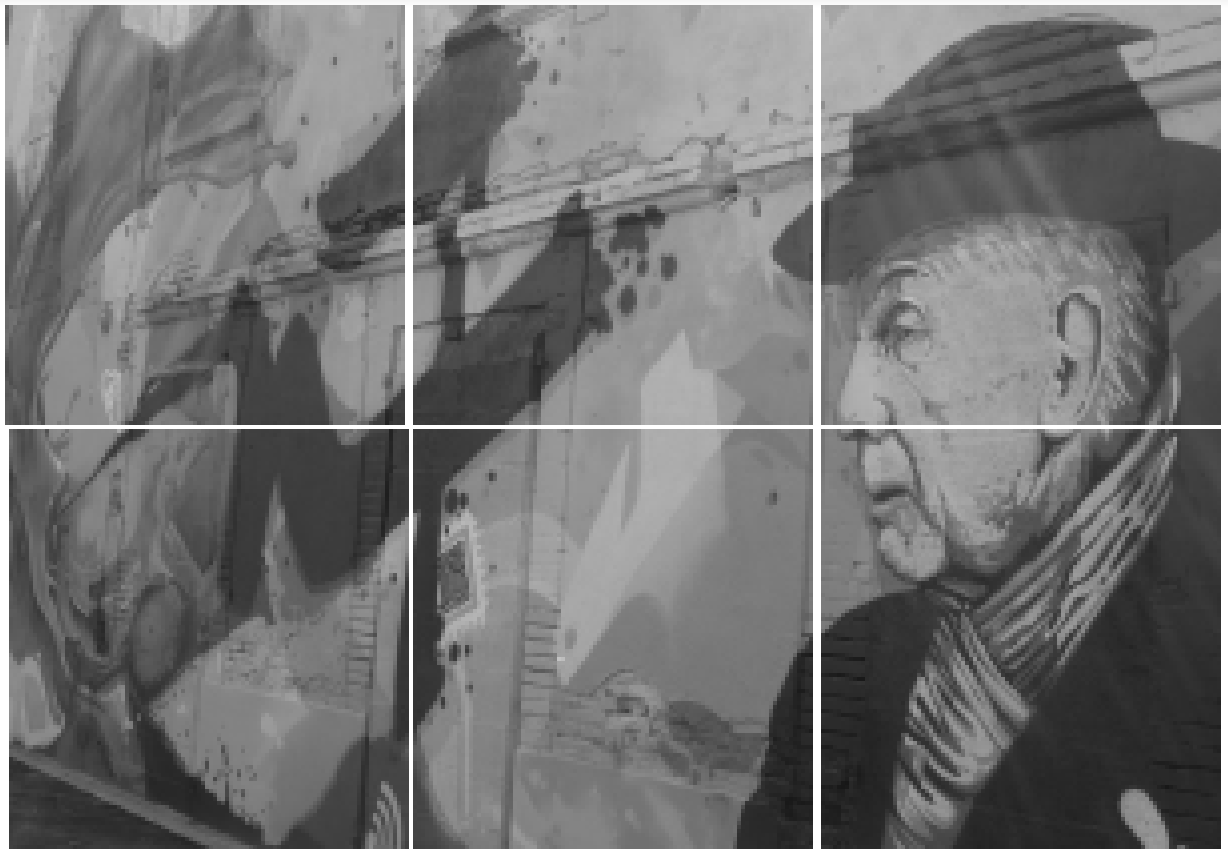
\includegraphics[width=0.5]{camichel.png}
\end{center}

Il s'agit du grand et fameux Charles Camichel ! Normalien de bonne facture, il fut prof d'élec à l'université de Lille de 1895 à 1900. En 1907, à la suite d'une dépression causée par le mauvais temps du nord de la France, il s'installe à Toulouse et crée l'institut électrotechique de Toulouse. Cette école évoluera jusqu'à avoir un nom beaucoup trop compliqué: école naionnale supérieure d'électrotechnique, d'électronique, d'informatique, d'hydraulique et des télécomunications. Heureusement, le groupe centrale est en route pour venir secourir cette école en perdition en la renomant "Institut Centrale Toulouse", faisant payer ce changement de nom aux élèves en mulltipliant par quatre les frais d'inscription.

% ne pas écrire en dessous

\begin{center}
    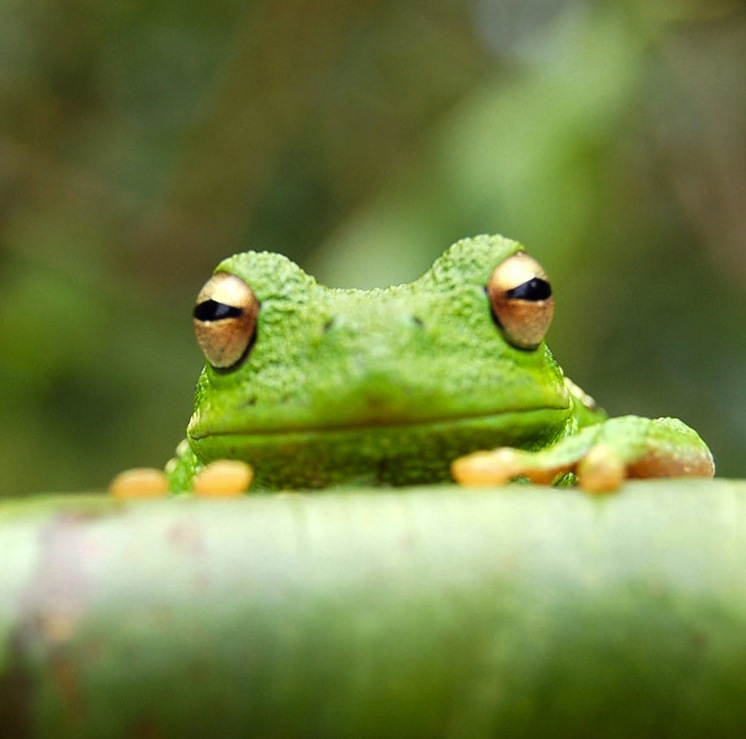
\includegraphics[width=0.125\textwidth]{frog.jpg}
\end{center}
\end{document}
